%% UTFPRCT-TEX, v1.0.6 wmeira on 2021/10/11
%% Copyright (C) 2020- by William H. T. Meira
%%
%% Modified version of project 'utfprpgtex' maintained 
%% by Luiz E. M. Lima
%%
%% This work may be distributed and/or modified under the
%% conditions of the LaTeX Project Public License, either version 1.3
%% of this license or (at your option) any later version.
%% The latest version of this license is in 
%%   http://www.latex-project.org/lppl.txt
%% and version 1.3 or later is part of all distributions of LaTeX
%% version 2005/12/01 or later.
%%
%% This work has the LPPL maintenance status `maintained'.
%%
%% The Current Maintainer of this work is William H. T. Meira.
%%
%% This project consists mainly of files: 'utfprct.cls', 'utfprct.tex', 
%% 'utfprct-dados.tex' 
%% 
%% The 'abntex2-alf.bst' and 'abntex2-num.bst' files are slightly
%% modified versions of the bibtex styles from abntex2 (v.1.9.7)
%% package to suit NBR6023/2018 (not yet implemented there). 
%% Complementary, 'abntex2-alf-en.bst' and 'abntex2-num-en.bst' are
%% english versions of the respective bibtex styles.
%%
%% Contribute to improve this project (github repo):
%% https://github.com/wmeira/utfprct-tex

%% Formato digital (sem folhas em branco): 
%% 'pretextualoneside': impressão dos elementos pré-textuais começa em qualquer lado da folha (anverso ou verso)
%% 'oneside': impressão dos elementos textuais e pós-textuais no anverso da folha (sem folhas em branco para o verso)

%% Formato impresso:
%% 'pretextualtwoside': impressão dos elementos pré-textuais começa sempre no anverso
%% 'oneside' ou 'twoside': impressão dos elementos textuais e pós-textuais `oneside` (anverso) ou `twoside` (anverso e verso, se mais de 100 páginas)

%% [Note] As legendas devem ser colocadas em cima do elemento (figura, tabela, quadro, algoritmo...) e os  \caption antes de entrar no ambiente. Obrigatoriamente, \fonte deve ser embaixo da elemento. Se for de criação do próprio autor, colocar "Autoria Própria." (Own Authorship.)
%\begin{figure}[htb]%% Ambiente figure
%\caption{Exemplo de caption}%% Legenda
%\label{fig:figura1}%% Rótulo
%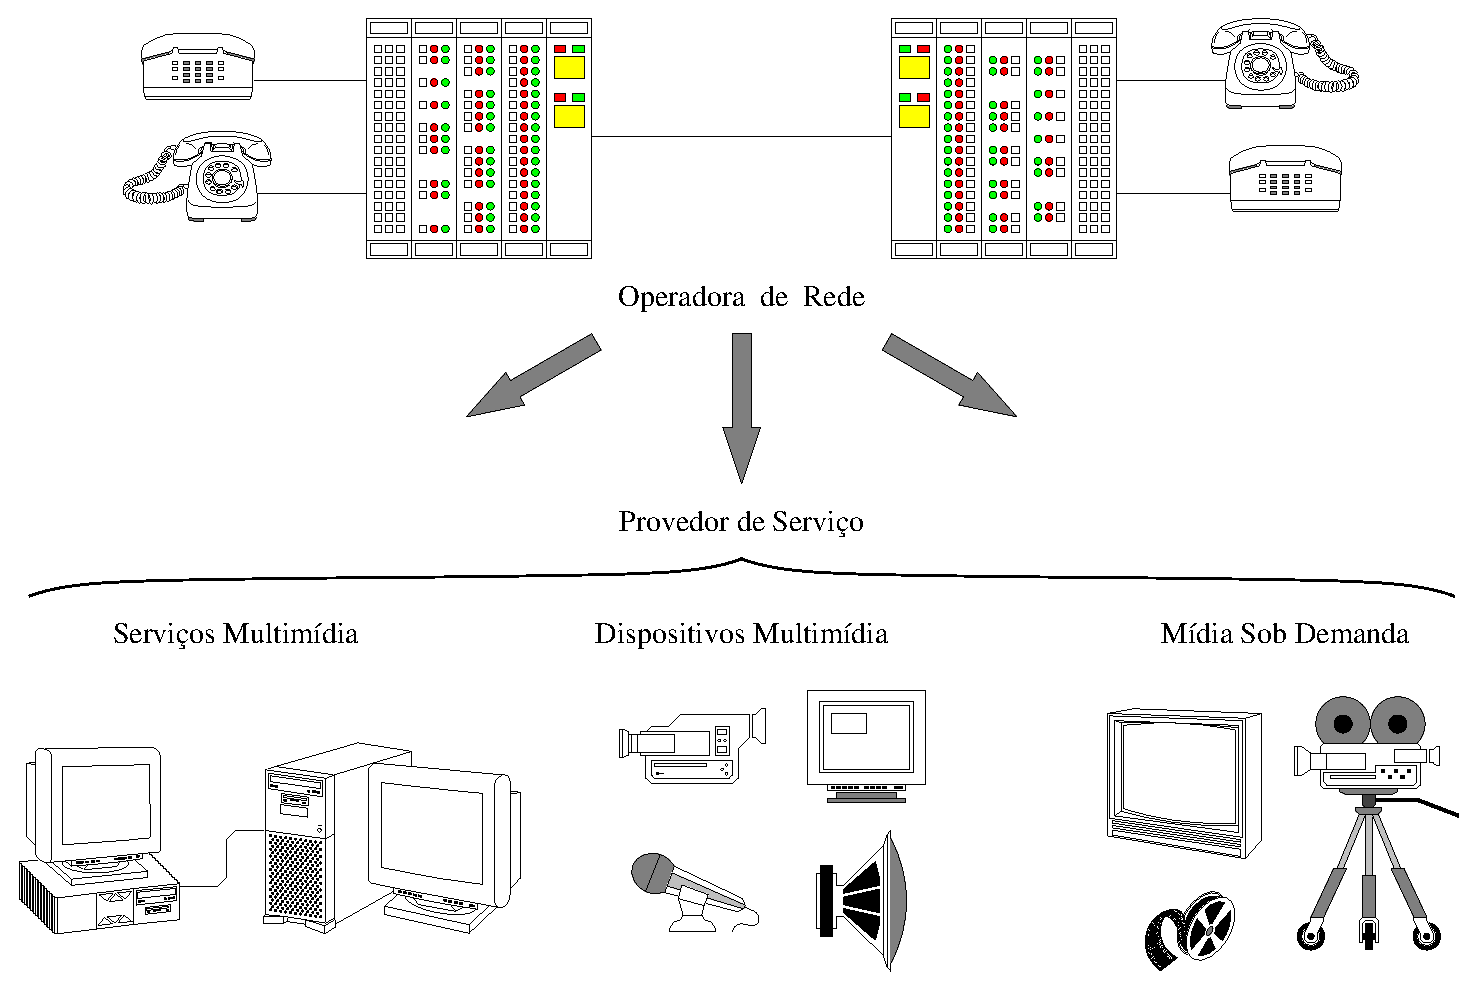
\includegraphics[width=\textwidth]{./CapituloExemplo/figura1}%% Dimensões e localização
%\fonte{\citet{Larsson2003}.}%% Fonte (quando criado pelo autor, usar Autoria Própria)
%\end{figure}

%% Classe e opções de documento
\documentclass[%% Opções
%% -- Opções da classe MEMOIR --
  12pt,%% Tamanho da fonte: 10pt, 11pt, 12pt, etc.
  a4paper,%% Tamanho do papel: a4paper (A4), letterpaper (carta), etc.
  % fleqn,%% Alinhamento das equações à esquerda (comente para alinhamento centralizado)
  % leqno,%% Numeração das equações no lado esquerdo (comente para lado direito)
  oneside,%% IMPRESSÃO dos elementos textuais e pós-textuais: oneside (apenas no anverso) ou twoside (anverso e verso, se mais de 100 p.) (insere páginas em branco).
%%  
%% -- Opções da classe ABNTEX2 --
  sumario = abnt-6027-2012,%% Formatação do sumário: tradicional (estilo tradicional) ou abnt-6027-2012 (norma ABNT 6027-2012)
  chapter = TITLE,%% Títulos de capítulos em maiúsculas (comente para desabilitar)
  section = TITLE,%% Títulos de seções secundárias em maiúsculas (comente para desabilitar)
  % subsection = TITLE,%% Títulos de seções terciárias em maiúsculas (comente para desabilitar)
  % subsubsection = TITLE,%% Títulos de seções quartenárias em maiúsculas (comente para desabilitar)
%%  
%% -- Opções da classe UTFPRCT-TEX --
  pretextualoneside,%% Impressão dos elementos pré-textuais: pretextualoneside (anverso) ou pretextualtwoside (anverso e verso)
  fontetimes,%% Fonte do texto: fontetimes (times), fontearial (arial) ou fontecourier (courier), fontemodern (lmodern - default latex). Times and Arial are ABNT recommended
   %vinculoscoloridos,%% Cores nos vínculos (citações, arquivos, links, url, etc.) (comente para desabilitar). NBR 14724/2011: cor preta (inclusive hyperlinks)
  semrecuonosumario,%% Remoção do recuo dos itens no sumário (comente para adição do recuo, se estilo tradicional)
  %inserirbackref,%% Inserir backref na lista de referências (e.g., Citado na página...)
  usemakeindex,%% Compilação de glossários e índices utilizando makeindex (comente para desabilitar)
  legendascentralizadas,%% Alinhamento das legendas centralizado (comente para alinhamento à esquerda)
%%  
%% -- Opções da folha de aprovação -- 
%% O mais comum é anexar o PDF do termo de aprovação sem assinaturas. As opções abaixo são para o formato da pós-graduação UTFPR-PG (Ponta Grossa) e podem servir de placeholder para este template.
  %aprovacaoestiloppg,%% Folha de aprovação do programa de pós-graduação no estilo do PPG (comente para estilo padrão)
  %pardeassinaturas,%% Assinaturas na folha de aprovação em até duas colunas (comente para em uma única coluna)
  % linhasdeassinaturas,%% Linhas de assinaturas na folha de aprovação (comente para remover as linhas)
%%  
%% -- Opções do pacote babel (hifenização) -- % 
  %french,%% Idioma adicional para hifenização (suporte parcial)
  %spanish,%% Idioma adicional para hifenização (suporte parcial)
  english,%% Idioma adicional para hifenização  (colocar em último para doc. em inglês)  
  brazil%% Idioma principal do documento (último da lista) 
]{utfprct_RedarTex}%% Classe utfprct

%%%%%%%%
% Documento em Inglês: colocar o "english" como último idioma carregado no documentclass, sendo o último a língua principal do documento.
%%%%%%%%

%%%%%%%%
%% Configuração dos avisos (warnings)
%% Comportamento do Tex quando um PDF é incluído e possui uma versão mais nova que a versão mínima especificada em \pdfminorversion. Opções: -1 (no info), 0 (default, warning), 1 (error)
\pdfinclusionerrorlevel=-1%no warning 
%\pdfminorversion=5%pdf minor output version (default 5)

%% [Badbox] Underfull e Overfull nível de aviso (filtra o que está abaixo)
\hbadness=5000%0 até 10000 (max) nível de badness
\vbadness=1000%0 até 10000 (max) nível de badness
%\hfuzz=0.01pt%excesso permitido de largura (\hbox)para ser considerado overfull
%\vfuzz=0.001pt%excesso permitido de altura (\vbox) para ser considerado overfull
%\overfullrule=10mm%adicionar aviso visual para um badbox
%%%%%%%%

%%%%%%%%
%% Pacotes carregados nas classes:
%%   memoir: abstract, appendix, array, booktabs, ccaption, chngcntr, chngpage, dcolumn, delarray, enumerate, epigraph, framed, ifmtarg, ifpdf, index, makeidx, moreverb, needspace, newfile, nextpage, parskip, patchcmd, setspace, shortvrb, showidx, tabularx, titleref, titling, tocbibind, tocloft, verbatim, verse.
%%   memoir (similares): crop, fancyhdr, geometry, sidecap, subfigure, titlesec.
%%   abntex2: babel, bookmark, calc, enumitem, ifthen, hyperref, textcase.
%%   utfprct: abntex2cite, ae, algorithmic, amsmath, backref, breakurl, caption, subcaption, cmap, color, eepic, epic, epsfig, etoolbox, fancyhdr, fix-cm, fontenc, glossaries, graphics, graphicx, helvet, hyphenat, indentfirst, inputenc, lastpage, morewrites, nomencl, sfmath, sistyle, substr, times, xtab, pdfpages.

%% Pacotes adicionais (\usepackage[options]{package})

\usepackage[autostyle=false, style=english]{csquotes}
\MakeOuterQuote{"}
\usepackage{bigdelim, booktabs, colortbl, longtable, multirow}%% Ferramentas para tabelas
\usepackage{amssymb, amstext, amsthm, icomma}%% Ferramentas para linguagem matemática
\usepackage{pifont, textcomp, wasysym}%% Símbolos de texto

%% inseridos por Victor Mammana
\let\newfloat\undefined %% evita o erro de recarregar newfloat
\usepackage{float}              % Fixa tabelas e figuras no local exato
\usepackage{graphicx}
\usepackage[export]{adjustbox}
\usepackage[skip=2pt,font=scriptsize]{caption}
\usepackage{subcaption}
\usepackage{soul}


% Refinamento tipográfico: diminui badboxes
\usepackage{microtype}%
\usepackage{chemfig,chemmacros} % Para escrever rea\c{c}\~oes qu\'{\i}micas
\usepackage{tikz}               % Para escrever rea\c{c}\~oes qu\'{\i}micas e outros
\usetikzlibrary{positioning}
\usetikzlibrary{er}

\usepackage{microtype}          % para melhorias de justifica\c{c}\~ao
\usepackage{pdfpages}
\usepackage{makeidx}            % para gerar \'{\i}ndice remissivo
\usepackage{hyphenat}          % Pacote para retirar a hifenizacao do texto
\usepackage[absolute]{textpos} % Pacote permite o posicionamento do texto
\usepackage{eso-pic}           % Pacote para incluir imagem de fundo
\usepackage{makebox}           % Pacote para criar caixa de texto



%% Comandos personalizados (\newcommand{name}[num]{definition})
\newcommand{\cpp}{\texttt{C$++$}}%% C++
\newcommand{\latex}{\LaTeX}%% LaTeX
\newcommand{\ds}{\displaystyle}%% Tamanho normal das equações
\newcommand{\bsym}[1]{\boldsymbol{#1}}%% Texto no modo matemático em negrito
\newcommand{\mr}[1]{\mathrm{#1}}%% Texto no modo matemático normal (não itálico)
\newcommand{\der}{\mr{d}}%% Operador diferencial
\newcommand{\deri}[2]{\frac{\der#1}{\der#2}}%% Derivada ordinária
\newcommand{\derip}[2]{\frac{\partial#1}{\partial#2}}%% Derivada parcial
\newcommand{\pare}[1]{\left(#1\right)}%% Parênteses
\newcommand{\colc}[1]{\left[#1\right]}%% Colchetes
\newcommand{\chav}[1]{\left\lbrace#1\right\rbrace}%% Chaves
\newcommand{\sen}{\operatorname{sen}}%% Operador seno
\newcommand{\senh}{\operatorname{senh}}%% Operador seno hiperbólico
\newcommand{\tg}{\operatorname{tg}}%% Operador tangente
\newcommand{\tgh}{\operatorname{tgh}}%% Operador tangente hiperbólico  
\ifthenelse{\equal{\languagename}{english}}{%%
\newcommand{\nomeequacao}{Equation}
\newcommand{\nomeequacoes}{Equations}
}{%default pt
\newcommand{\nomeequacao}{Equação}
\newcommand{\nomeequacoes}{Equações}
}%  
\newcommand{\seqref}[1]{\nomeequacao~\eqref{#1}}%% Referência de uma única equação
\newcommand{\meqref}[1]{\nomeequacoes~\eqref{#1}}%% Referência de multiplas equações
\newcommand{\citep}[1]{\cite{#1}}%% Atalho para citação implícita
\newcommand{\citet}[1]{\citeonline{#1}}%% Atalho para citação explícita
\newcommand{\citepa}[1]{(\citeauthor{#1})}%% Atalho para citação implícita (somente autor)
\newcommand{\citeta}[1]{\citeauthoronline{#1}}%% Atalho para citação explícita (somente autor)
\newcommand{\citepy}[1]{(\citeyear{#1})}%% Atalho para citação implícita (somente ano)
\newcommand{\citety}[1]{\citeyear{#1}}%% Atalho para citação explícita (somente ano)

%allow fixed size on collums with text position
\newcolumntype{L}[1]{>{\raggedright\let\newline\\\arraybackslash\hspace{0pt}}m{#1}}
\newcolumntype{C}[1]{>{\centering\let\newline\\\arraybackslash\hspace{0pt}}m{#1}}
\newcolumntype{R}[1]{>{\raggedleft\let\newline\\\arraybackslash\hspace{0pt}}m{#1}}

%%%%%%%%%%%%%%%%%%%%%%%%%%%%%%%%%%%%%%%%%%%%%%%
%%%%%%%%%%%%%%%%%%%%%%%%%%%%%%%%%%%%%%%%%%%%%%%
%% Configuração das entradas
%%

%% Arquivo de dados do modelo de documento LaTeX para produção de trabalhos acadêmicos da UTFPR
%% UTFPRCT-TEX, v1.0.6 wmeira on 2021/10/11
%% Copyright (C) 2020- by William H. T. Meira
%%
%% Modified version of project 'utfprpgtex' maintained 
%% by Luiz E. M. Lima
%%
%% Alterado por Victor Mammana
%%
%% This work may be distributed and/or modified under the
%% conditions of the LaTeX Project Public License, either version 1.3
%% of this license or (at your option) any later version.
%% The latest version of this license is in
%%   http://www.latex-project.org/lppl.txt
%% and version 1.3 or later is part of all distributions of LaTeX
%% version 2005/12/01 or later.
%%
%% This work has the LPPL maintenance status `maintained'.
%%
%% The Current Maintainer of this work is William H. T. Meira.
%%
%% This project consists mainly of files: 'utfprct.cls', 'utfprct.tex', 
%% 'utfprct-dados.tex' 
%% 
%% The 'abntex2-alf.bst' and 'abntex2-num.bst' files are slightly
%% modified versions of the bibtex styles from abntex2 (v.1.9.7)
%% package to suit NBR6023/2018 (not yet implemented there). 
%% Complementary, 'abntex2-alf-en.bst' and 'abntex2-num-en.bst' are
%% english versions of the respective bibtex styles.
%%
%% Contribute to improve this project (github repo):
%% https://github.com/wmeira/utfprct-tex

%%%%%%%%%%%%%%%%%%%%%%%%%%%%%%%%%%%%%%%%%%%%%%%
%%%%%%%%%%%%%%%%%%%%%%%%%%%%%%%%%%%%%%%%%%%%%%%
%% Tutorial do Documento de Dados 
%%%%%%%%%%%%%%%%%%%%%%%%%%%%%%%%%%%%%%%%%%%%%%%
%%
%% O 'utfprct-dados.tex' cont\'em todos as informa\c{c}\~oes do documento, 
%% metadados e outros valores importantes para o preenchimento dos 
%% elementos pr\'e-textuais: capa, folha de rosto, resumo, abstract.
%% 
%% N\~ao \'e necess\'ario preencher todos os campos, existem campos mais
%% espec\'{\i}ficos para o tipo de documento sendo elaborado. Quando TCC,
%% por exemplo, n\~ao \'e necess\'ario definir dados do programa de 
%% p\'os-gradua\c{c}\~ao. Todos os dados inseridos estar\~ao dispon\'{\i}veis para
%% inser\c{c}\~ao no tex usando o padr\~ao '\imprimir + nomedodadominusculo'. 
%% Por exemplo, para imprimir o tipo do documento ('\TipoDeDocumento'),
%% usar '\imprimirtipodedocumento'.
%%
%% \'E poss\'{\i}vel customizar a descri\c{c}\~ao do documento na folha de rosto. 
%% Exemplos de descri\c{c}\~ao s\~ao fornecidos para guiar a escrita do texto,
%% em que pode-se utilizar os dados j\'a definidos com o padr\~ao descrito.
%%
%% Existe a possibilidade de inserir dados de uma institui\c{c}\~ao de 
%% cotutela quando se aplicar. 
%%
%% Os dados da ficha catalogr\'afica s\~ao fornecidos pela biblioteca
%% e, na maioria das vezes, apenas anexa-se a folha digitalizada
%% na regi\~ao definida dos elementos pr\'e-textuais.
%%
%% A folha de aprova\c{c}\~ao \'e, na maioria das vezes, fornecido 
%% digitalmente pelo departamento ou pelo orientador ap\'os a defesa e 
%% dever\'a ser anexada ao documento na regi\~ao definida dos elementos 
%% pr\'e-textuais. Recomenda-se apenas anexar a folha de aprova\c{c}\~ao sem
%% precisar alterar os dados espec\'{\i}ficos aqui presentes, pois foram
%% criados originalmente para o template da folha de aprova\c{c}\~ao da
%% UTFPR-PG, presente no projeto base, e foram apenas mantidos.
%%
%%%%%%%%%%%%%%%%%%%%%%%%%%%%%%%%%%%%%%%%%%%%%%%
%%%%%%%%%%%%%%%%%%%%%%%%%%%%%%%%%%%%%%%%%%%%%%%

%%%%%%%%%%%%%%%%%%%%%%%%%%%%%%%%%%%%%%%%%%%%%%%
%% Informa\c{c}\~oes do Documento
%%%%%%%%%%%%%%%%%%%%%%%%%%%%%%%%%%%%%%%%%%%%%%%

%% Tipo de documento (op\c{c}\~oes: "Tese", "Disserta\c{c}\~ao", "Trabalho de Conclus\~ao de Curso"
\TipoDeDocumento{Disserta\c{c}\~ao}%copiar exatamente uma das op\c{c}\~oes 

%% [abstract] Document type: "Thesis", "Dissertation", "Bachelor Thesis"
\DocumentType{Dissertation}%

%% N\'{\i}vel de forma\c{c}\~ao: "Doutorado", "Mestrado", "Bacharelado"
\NivelDeFormacao{Mestrado}%

%% [abstract] Formation level: "Doctorate", "PhD", "Master's Degree", "Bachelor's Degree"
\FormationLevel{Msc.}%

%% T\'{\i}tulo ou grau pretendido: "Doutor", "Mestre" ou "Bacharel"
\TituloPretendido{@[mestreoudoutor]@}%

%%%%%%%%%%%%%%%%%%%%%%%%%
%% Por padr\~ao, o t\'{\i}tulo principal ser\'a o \TituloDoDocumento (portugu\^es)
%% Se a l\'{\i}ngua do documento for definida como ingl\^es, ser\'a o \DocumentTitle

%% T\'{\i}tulo do documento em PORTUGU\^ES (resumo)
\TituloDoDocumento{%%
@[titulo]@ %% : @[subtitulo]@ coloque se tiver subtitulo
}%

%% T\'{\i}tulo do trabalho em INGL\^ES (abstract)
\DocumentTitle{%%
@[tituloabstract]@
}%

%% T\'{\i}tulo em m\'ultiplas linhas na capa, folha de rosto e termo de aprova\c{c}\~ao
%% Use o comando \par para indicar a quebra de linha
%%
%% A CAPA apresentar\'a o t\'{\i}tulo no formato de m\'ultiplas linhas
%% para a respectiva l\'{\i}ngua do documento definida.
%%
%% Na folha de rosto, caso a l\'{\i}ngua do documento n\~ao seja portugu\^es, aparecer\'a o
%% \TituloEmMultiplasLinhasIngles seguido pela tradu\c{c}\~ao \TituloEmMultiplasLinhas
%%
\TituloEmMultiplasLinhas{%%
@[titulo]@ %%\par coloque se tiver subtitulo
%% @[subtitulo]@ coloque se tiver subtitulo
}%

\TituloEmMultiplasLinhasIngles{%%
@[tituloabstract]@ %% \par coloque se tiver subtitulo
%%subtitle of this academic work
}%

%%%%%%%%%%%%%%%%%%%%%%%%%


%% Data da defesa
\Dia{10}%% Dia (opcional: usado na ficha catalogr\'afica apenas)
\MesPorExtenso{mar\c{c}o}%% m\^es por extenso (opcional: usado na ficha catalogr\'afica apenas)
\Ano{@[ano]@}%% Ano

%% Palavras-chave e keywords (m\'aximo 5)
\NumeroDePalavrasChave{5}%% N\'umero de palavras-chave 
\PalavraChaveA{Papert}%% Palavra-chave A
\PalavraChaveB{STEAM}%% Palavra-chave B
\PalavraChaveC{STEM}%% Palavra-chave C
\PalavraChaveD{WASH}%% Palavra-chave D
\PalavraChaveE{Educa\c{c}\~ao}%% Palavra-chave E

\NumeroDeKeywords{\imprimirnumerodepalavraschave}%% N\'umero de keywords (mesmo que palavras-chave)
\KeywordA{Papert}%% Keyword A
\KeywordB{STEAM}%% Keyword B
\KeywordC{STEM}%% Keyword C
\KeywordD{WASH}%% Keyword D
\KeywordE{Education}%% Keyword E

%%%%%%%%%%%%%%%%%%%%%%%%%%%%%%%%%%%%%%%%%%%%%%%
%% Informa\c{c}\~ao do Autor(a) ou Autores(as) (TCC)
%%%%%%%%%%%%%%%%%%%%%%%%%%%%%%%%%%%%%%%%%%%%%%%

%%% Autor(a)
%% Usado para cita\c{c}\~ao: "\SobrenomeDoAutor, PrenomeDoAutor" (ex: "Doe, John" ou "Doe, J.")
\NomeDoAutor{@[autor]@}%% Nome completo do(a) autor(a)
\SobrenomeDoAutor{@[ultimonome]@}%% \'Ultimo nome do(a) autor(a)
\PrenomeDoAutor{@[primeirosnomes]@}%% Nome do(a) autor(a) sem \'ultimo nome

%%% Autor(a) 2 (opcional)
%% *Considera apenas se "\TipoDeDocumento" == "Trabalho de Conclus\~ao de Curso"
\AtribuiAutorDois{false}%% Insere ou remove autor(a) 2: "true" ou "false"
\NomeDoAutorDois{Nome do(a) Autor(a) 2}%% Nome completo do(a) autor(a) 2
\SobrenomeDoAutorDois{\'Ultimo Nome}%% \'Ultimo nome do(a) autor(a) 2
\PrenomeDoAutorDois{Nome do(a) Autor(a) 2 Sem \'Ultimo}%% Nome do(a) autor(a) 2 sem \'ultimo nome

%%% Autor(a) 3 (opcional)
%% *Considera apenas se "\TipoDeDocumento" == "Trabalho de Conclus\~ao de Curso"
\AtribuiAutorTres{false}%% Insere ou remove autor(a) 3: "true" ou "false"
\NomeDoAutorTres{Nome do(a) Autor(a) 3}%% Nome completo do(a) autor(a) 3
\SobrenomeDoAutorTres{\'Ultimo Nome}%% \'Ultimo nome do(a) autor(a) 3
\PrenomeDoAutorTres{Nome do(a) Autor(a) 3 Sem \'Ultimo}%% Nome do(a) autor(a) 3 sem \'ultimo nome

%%%%%%%%%%%%%%%%%%%%%%%%%%%%%%%%%%%%%%%%%%%%%%%%%%
%% Informa\c{c}\~oes do Orientador(a) e Coorientador(a)
%%%%%%%%%%%%%%%%%%%%%%%%%%%%%%%%%%%%%%%%%%%%%%%%%%

%% Orientador(a)
%% Usado para cita\c{c}\~ao: "\SobrenomeDoOrientador, PrenomeDoOrientador" (ex: "Doe, John" ou "Doe, J.")
\AtribuicaoOrientador{Orientador}%% Atribui\c{c}\~ao "Orientador(a)"
\TituloDoOrientador{Prof. Dr.}%% T\'{\i}tulo do(a) orientador(a)
\NomeDoOrientador{@[orientador]@}%% Nome completo do(a) orientador(a)
\SobrenomeDoOrienador{@[ultimonomeorientador]@}%% \'Ultimo nome do(a) orientador(a)
\PrenomeDoOrientador{@[primeirosnomesorientador]@}%% Nome do(a) orientador(a) sem \'ultimo nome

%% Coorientador(a) (opcional)
%% Usado para cita\c{c}\~ao: "\SobrenomeDoCoorientador, PrenomeDoCoorientador" (ex: "Doe, John" ou "Doe, J.")
\AtribuiCoorientador{true}%% Insere ou remove o(a) coorientador(a): "true" ou "false"
\AtribuicaoCoorientador{Coorientador}%% Atribui\c{c}\~ao "Coorientador(a)"
\TituloDoCoorientador{Prof. Dr.}%% T\'{\i}tulo do(a) coorientador(a)
\NomeDoCoorientador{@[coorientador]@}%% Nome completo do(a) coorientador(a)
\SobrenomeDoCoorienador{@[ultimonomecoorientador]@}%% \'Ultimo nome do(a) coorientador(a)
\PrenomeDoCoorientador{@[primeirosnomescoorientador]@}%% Nome do(a) coorientador(a) sem \'ultimo nome

%%%%%%%%%%%%%%%%%%%%%%%%%%%%%%%%%%%%%%%%%%%%%%%%%%
%% Informa\c{c}\~oes da Institui\c{c}\~ao
%%%%%%%%%%%%%%%%%%%%%%%%%%%%%%%%%%%%%%%%%%%%%%%%%%

%% Nome da institui\c{c}\~ao
\Instituicao{@[universidade]@}

%% [abstract] Institution name (*nome sem traduzir \'e o recomendado para docs. da UTFPR)
\Institution{@[universidade]@}

%% Sigla da Institui\c{c}\~ao
\SiglaInstituicao{@[universidademaiuscula]@}

%% Nome da cidade (c\^ampus)
\Cidade{@[localidade]@}

%% Diretoria: "Gradua\c{c}\~ao e Educa\c{c}\~ao Profissional" ou "Pesquisa e P\'os-Gradua\c{c}\~ao" (opcional)
\Diretoria{Pesquisa e P\'os-Gradua\c{c}\~ao}

%% Nome do departamento ou da coordena\c{c}\~ao (opcional: mais comum no Bacharelado: Departamento de Inform\'atica)
\Departamento{@[programapos]@}

%% Sigla do departamento (opcional, ex: DAINF, DAMEC, DAMAT...)
\SiglaDepartamento{PPGEN}

%% Nome do curso bachalerado ou p\'os-gradua\c{c}\~ao (PPG) (ex: "Engenharia de Computa\c{c}\~ao",  "Engenharia El{\'e}trica e Inform{\'a}tica Industrial") 
\Curso{@[titulopos]@}

%% [abstract] Course name
\Course{Teaching Social, Human and Natural Sciences}

%% Programa ou nome do curso completo (capa)
%% "Bachalerado em Engenharia de Computa\c{c}\~ao"
%% "@[programapos]@
\Programa{@[programapos]@}

%% Sigla do programa de p\'os-gradua\c{c}\~ao (opcional, ex: CPGEI, PPGCA)
\SiglaDoPPG{PPGEN}

%% Nome da \'area de concentra\c{c}\~ao
\AreaDeConcentracao{Educa\c{c}\~ao}

%%%%%%%%%%%%%%%%%%%%%%%%%%%%%%%%%%%%%%%%%%%%%%%%%%%%%%
%% Informa\c{c}\~oes de Cotutela (Duplo Grau) (opcional)
%%%%%%%%%%%%%%%%%%%%%%%%%%%%%%%%%%%%%%%%%%%%%%%%%%%%%%

%% Insere dados de cotutela: "true" ou "false"
\AtribuiCotutela{false}

%% Nome da institui\c{c}\~ao de cotutela
\InstituicaoCotutela{Universidade Da Cotutela}

%% [abstract] Institution name
\InstitutionCotutela{Double Degree University}

%% Sigla da institui\c{c}\~ao de cotutela
\SiglaInstituicaoCotutela{UC}

%% Nome do departamento ou da coordena\c{c}\~ao da inst. de cotutela (mais comum no Bacharelado: Departamento de Inform\'atica)
\DepartamentoCotutela{Nome do Departamento ou da Coordena\c{c}\~ao}

%% Sigla do departamento da inst. cotutela (ex: DAINF, DAMEC, DAMAT...)
\SiglaDepartamentoCotutela{DPT-EXT}

%% Nome do curso bachalerado ou p\'os-gradua\c{c}\~ao (PPG) na institui\c{c}\~ao de cotutela (ex: "Engenharia de Computa\c{c}\~ao",  "Engenharia El{\'e}trica e Inform{\'a}tica Industrial")
\CursoCotutela{Nome do @[curso]@}

%% [abstract] Course name 
\CourseCotutela{Second Degree Course}

%% Programa ou nome do curso completo na inst. cotutela (capa)
%% "Bachalerado em Engenharia de Computa\c{c}\~ao"
%% "@[programapos]@
\ProgramaCotutela{Programa de Doutoral em \imprimircursocotutela}

%% Sigla do programa externo de p\'os-gradua\c{c}\~ao
\SiglaDoPPGCotutela{PPG-EXT}

%% Nome da \'area de concentra\c{c}\~ao na institui\c{c}\~ao de cotutela
\AreaDeConcentracaoCotutela{Nome da \'Area de Concentra\c{c}\~ao}

%% N\'{\i}vel de forma\c{c}\~ao que ser\'a fornecido na refer\^encia do doc.
\NivelDeFormacaoResumo{Duplo doutorado}
\FormationLevelAbstract{Double PhD}

%% Informacoes do orientador(a) na institui\c{c}\~ao de cotutela

%% Orientador(a) da institui\c{c}\~ao de cotutela
%% Usado para cita\c{c}\~ao: "\SobrenomeDoOrientador, PrenomeDoOrientador" (ex: "Doe, John" ou "Doe, J.")
\AtribuicaoOrientadorCotutela{Orientador(a)}%% Atribui\c{c}\~ao "Orientador(a)"
\TituloDoOrientadorCotutela{Prof(a). Dr(a).}%% T\'{\i}tulo do(a) orientador(a)
\NomeDoOrientadorCotutela{Nome Completo do(a) Orientador(a)}%% Nome completo do(a) orientador(a)
\SobrenomeDoOrienadorCotutela{\'Ultimo Nome}%% \'Ultimo nome do(a) orientador(a)
\PrenomeDoOrientadorCotutela{Nome do(a) Orientador(a) Sem \'Ultimo}%% Nome do(a) orientador(a) sem \'ultimo nome

%% Coorientador(a) da institui\c{c}\~ao de cotutela
%% Usado para cita\c{c}\~ao: "\SobrenomeDoCoorientador, PrenomeDoCoorientador" (ex: "Doe, John" ou "Doe, J.")
\AtribuiCoorientadorCotutela{false}%% Insere ou remove o(a) coorientador(a) da cotutela: "true" ou "false"
\AtribuicaoCoorientadorCotutela{Coorientador(a)}%% Atribui\c{c}\~ao "Coorientador(a)"
\TituloDoCoorientadorCotutela{Prof(a). Dr(a).}%% T\'{\i}tulo do(a) coorientador(a)
\NomeDoCoorientadorCotutela{Nome Completo do(a) Coorientador(a)}%% Nome completo do(a) coorientador(a)
\SobrenomeDoCoorienadorCotutela{\'Ultimo Nome}%% \'Ultimo nome do(a) coorientador(a)
\PrenomeDoCoorientadorCotutela{Nome do(a) Coorientador(a) Sem \'Ultimo}%% Nome do(a) coorientador(a) sem \'ultimo nome

%%%%%%%%%%%%%%%%%%%%%%%%%%%%%%%%%%%%%%%%%%%%%%%%%%
%% Folha de Rosto
%%%%%%%%%%%%%%%%%%%%%%%%%%%%%%%%%%%%%%%%%%%%%%%%%%

%% Se desejar usar os dados inseridos, eles est\~ao dispon\'{\i}ves
%% usando o padr\~ao '\imprimir + nomedodadominusculo'. Por exemplo,
%% para imprimir o tipo do documento ('\TipoDeDocumento'), usar
%% '\imprimirtipodedocumento'

%% Descri\c{c}\~ao do documento na folha de rosto (exemplos)
\DescricaoDoDocumento{
\imprimirtipodedocumento\ apresentada como requisito para obten\c{c}\~ao do t\'{\i}tulo de \imprimirtitulopretendido\ em \imprimircurso, do \imprimirppgoudepartamento, da \imprimirinstituicao\ (\imprimirsiglainstituicao).
}

% Exemplo: Mestrado
%\DescricaoDoDocumento{
%\imprimirtipodedocumento\ apresentada como requisito para obten\c{c}\~ao do grau de \imprimirtitulopretendido\ em \imprimircurso\ da \imprimirinstituicao\ (\imprimirsiglainstituicao).
%}

% Exemplo: Doutorado
%\DescricaoDoDocumento{
%\imprimirtipodedocumento\ apresentada como requisito para obten\c{c}\~ao do t\'{\i}tulo de \imprimirtitulopretendido\ em \imprimircurso\ da \imprimirinstituicao\ (\imprimirsiglainstituicao).
%}


%% Insere ou remove descri\c{c}\~ao da cotutela (extra) na folha de rosto: "true" ou "false". 
%% Se "true", a descri\c{c}\~ao do documento ser\'a colocada na folha de rosto, logo abaixo do orientador(a) e coorientador(a) da primeira inst. e depois o orientador(a) e coorientador(a) da inst. de cotutela. 
%% Se "false", os nomes do orientador(a) e coorientador(a) aparecer\~ao logo abaixo do orientador(a) da primeira institui\c{c}\~ao, sem uma descri\c{c}\~ao extra. Neste caso, recomenda-se revisar a "\DescricaoDoDocumento" para contemplar ambas as institui\c{c}\~oes.   
\AtribuiDescricaoCotutela{false}

%% Segunda Descricao da Inst. de Cotutela na folha de rosto (exemplos)
\DescricaoDoDocumentoCotutela{
\imprimirtipodedocumento\ apresentado(a) como requisito \`a obten\c{c}\~ao do t\'{\i}tulo de \imprimirtitulopretendido\ em \imprimircursocotutela, do \imprimirppgoudepartamentocotutela, da \imprimirinstituicaocotutela.  
%\imprimirtipodedocumento\ apresentada \`a Comiss\~ao de Acompanhamento de Tese do Programa Doutoral em \imprimircursocotutela\ do \imprimirinstituicaocotutela\ (\imprimirsiglainstituicaocotutela) como requisito \`a obten\c{c}\~ao de grau de \imprimirtitulopretendido\ na \'area de concentra\c{c}\~ao \imprimirareadeconcentracaocotutela.
}

%%%%%%%%%%%%%%%%%%%%%%%%%%%%%%%%%%%%%%%%%%%%%%%%%%
%% Ficha Catalogr\'afica* (opcional)
%%%%%%%%%%%%%%%%%%%%%%%%%%%%%%%%%%%%%%%%%%%%%%%%%%

%% *Pode ser usado como placeholder, por\'em para entrega deve-se inserir a ficha catologr\'afica digitalizado (PDF) pela biblioteca da UTFPR.

\NumeroDaPublicacao{00/\imprimirano}%% N\'umero da publica\c{c}\~ao - Fornecido pela biblioteca
\CDDOuCDU{CDD 000.00}%% Classifica\c{c}\~ao Decimal Dewey (CDD) ou Classifica\c{c}\~ao Decimal Universal (CDU) - Fornecida pela biblioteca

\TituloDaFichaCatalografica{%% T\'{\i}tulo da ficha catalogr\'afica
  Ficha catalogr\'afica elaborada pelo Departamento de Biblioteca da \par \imprimirinstituicao, C\^ampus \imprimircidade \par n.
  \imprimirnumerodapublicacao
}

%%%%%%%%%%%%%%%%%%%%%%%%%%%%%%%%%%%%%%%%%%%%%%%%%%
%% Folha de aprova\c{c}\~ao (Formato UTFPR-PG)* (opcional)
%%%%%%%%%%%%%%%%%%%%%%%%%%%%%%%%%%%%%%%%%%%%%%%%%%

%% *Pode ser usado como placeholder, por\'em para entrega final prefere-se a folha (termo) de aprova\c{c}\~ao digitalizado (PDF) fornecido pelo departamento ou orientador.

\NumeroDaTeseOuDissertacao{00/\imprimirano}%% N\'umero da Tese ou Disserta\c{c}\~ao - Fornecido pelo programa de p\'os-gradua\c{c}\~ao
\NumeroDaFichaCatalografica{A000}%% N\'umero da ficha catalogr\'afica - Fornecido pela biblioteca

\TituloDoResponsavelTCC{Prof(a). Dr(a).}%% T\'{\i}tulo do(a) respons\'avel pelos TCC
\NomeDoResponsavelTCC{Nome do(a) Respons\'avel}%% Nome completo do(a) respons\'avel pelos TCC
\AtribuicaoCoordenador{Coordenador(a)}%% Atribui\c{c}\~ao "Coordenador(a)" do curso
\TituloDoCoordenador{Prof(a). Dr(a).}%% T\'{\i}tulo do(a) coordenador(a) do curso
\NomeDoCoordenador{Nome do(a) Coordenador(a)}%% Nome completo do(a) coordenador(a) do curso

\TextoDeAprovacao{%% Texto de aprova\c{c}\~ao
  %% Exemplo de texto de aprova\c{c}\~ao para Tese ou Disserta\c{c}\~ao (descomente a pr\'oxima linha para utiliz\'a-lo):
  Esta \imprimirtipodedocumento\ foi apresentada \`as 00:00 de \imprimirdia\ de \imprimirmesporextenso\ de \imprimirano\ como requisito parcial para a obten\c{c}\~ao do t\'{\i}tulo de \imprimirtitulopretendido\ em \imprimircurso, na \'area de concentra\c{c}\~ao em \imprimirareadeconcentracao\ e na linha de pesquisa em (Nome da Linha de Pesquisa), do @[programapos]@. O(A) candidato(a) foi arguido(a) pela Banca Examinadora composta pelos professores abaixo citados. Ap\'os delibera\c{c}\~ao, a Banca Examinadora considerou o trabalho aprovado.
  %% Exemplo de texto de aprova\c{c}\~ao para Trabalho de Conclus\~ao de @[curso]@\'oxima linha para utiliz\'a-lo):
  % Este \imprimirtipodedocumento\ foi apresentado em \imprimirdia\ de \imprimirmesporextenso\ de \imprimirano\ como requisito parcial para a obten\c{c}\~ao do t\'{\i}tulo de \imprimirtitulopretendido\ em \imprimircurso. O(A) candidato(a) foi arguido(a) pela Banca Examinadora composta pelos professores abaixo assinados. Ap\'os delibera\c{c}\~ao, a Banca Examinadora considerou o trabalho aprovado.
}

\AvisoDeAprovacao{%% Aviso de aprova\c{c}\~ao
  %% Exemplo de aviso de aprova\c{c}\~ao para Tese ou Disserta\c{c}\~ao (descomente a pr\'oxima linha para utiliz\'a-lo):
  A Folha de Aprova\c{c}\~ao assinada encontra-se no \par Departamento de Registros Acad\^emicos da UTFPR -- C\^ampus \imprimircidade
  %% Exemplo de aviso de aprova\c{c}\~ao para Trabalho de Conclus\~ao de @[curso]@\'oxima linha para utiliz\'a-lo):
  % -- O Termo de Aprova\c{c}\~ao assinado encontra-se na Coordena\c{c}\~ao do @[curso]@--
}

%% Banca examinadora: 3 membros (Trabalho de Conclus\~ao de @[curso]@\c{c}\~ao); 5 a 7 membros (Tese)
\MembroAIgualOrientador{true}%% Insere ou remove o membro A igual ao(\`a) orientador(a): "true" ou "false"
\MembroA{Nome do Membro A}%% Nome completo do membro A - Presidente (autom\'atico se orientador(a))
\TituloDoMembroA{Prof(a). Dr(a).}%% T\'{\i}tulo do membro A - Presidente (autom\'atico se orientador(a))
\InstituicaoDoMembroA{Institui\c{c}\~ao do Membro A}%% Nome da institui\c{c}\~ao do membro A - Presidente (autom\'atico se orientador(a))
\MembroB{Nome do Membro B}%% Nome completo do membro B
\TituloDoMembroB{Prof(a). Dr(a).}%% T\'{\i}tulo do membro B
\InstituicaoDoMembroB{Institui\c{c}\~ao do Membro B}%% Nome da institui\c{c}\~ao do membro B
\MembroC{Nome do Membro C}%% Nome completo do membro C
\TituloDoMembroC{Prof(a). Dr(a).}%% T\'{\i}tulo do membro C
\InstituicaoDoMembroC{Institui\c{c}\~ao do Membro C}%% Nome da institui\c{c}\~ao do membro C
\MembroD{Nome do Membro D}%% Nome completo do membro D
\TituloDoMembroD{Prof(a). Dr(a).}%% T\'{\i}tulo do membro D
\InstituicaoDoMembroD{Institui\c{c}\~ao do Membro D}%% Nome da institui\c{c}\~ao do membro D
\MembroE{Nome do Membro E}%% Nome completo do membro E
\TituloDoMembroE{Prof(a). Dr(a).}%% T\'{\i}tulo do membro E
\InstituicaoDoMembroE{Institui\c{c}\~ao do Membro E}%% Nome da institui\c{c}\~ao do membro E
\AtribuiMembroF{false}%% Insere ou remove o Membro F: "true" ou "false"
\MembroF{Nome do Membro F}%% Nome completo do membro F
\TituloDoMembroF{Prof(a). Dr(a).}%% T\'{\i}tulo do membro F
\InstituicaoDoMembroF{Institui\c{c}\~ao do Membro F}%% Nome da institui\c{c}\~ao do membro F
\AtribuiMembroG{false}%% Insere ou remove o Membro G: "true" ou "false"
\MembroG{Nome do Membro G}%% Nome completo do membro G
\TituloDoMembroG{Prof(a). Dr(a).}%% T\'{\i}tulo do membro G
\InstituicaoDoMembroG{Institui\c{c}\~ao do Membro G}%% Nome da institui\c{c}\~ao do membro G
%% Realize as modificações pertinentes no arquivo "utfprct-dados.tex"

%% Ferramenta para criação de índices
\makeindex%% Não comente esta linha

%% Ferramenta para criação de glossários
\makeglossaries%% Não comente esta linha

%% Entradas da lista de abreviaturas, siglas e acrônimos

%%%% LISTA DE ABREVIATURAS, SIGLAS E ACR\^ONIMOS
%%
%% Rela\c{c}\~ao, em ordem alfab\'etica, das abreviaturas (representa\c{c}\~ao de uma palavra por meio de alguma(s) de sua(s) s\'{\i}laba(s) ou
%% letra(s)), siglas (conjunto de letras iniciais dos voc\'abulos e/ou n\'umeros que representa um determinado nome) e acr\^onimos
%% (conjunto de letras iniciais dos voc\'abulos e/ou n\'umeros que representa um determinado nome, formando uma palavra pronunci\'avel).
%%
%%
%% Este arquivo para defini\c{c}\~ao de abreviaturas, siglas e acr\^onimos \'e utilizado com a op\c{c}\~ao \incluirlistadeacronimos{glossaries}
%%
%% Vantagens do modo com "glossaries" em rela\c{c}\~ao ao modo "file":
%%   1) Ordena automaticamente a lista
%%	 2) Apenas os termos referenciados s\~ao colocados na lista


%% Como referenciar: 
%% \gls{lp} = Linear Programming (LP)  (First use)
%% \gls{lp} = LP (Next uses)
%% \glspl{lp} = LPs
%% \glsentrytext{lp} = Linear Programming    (recommended for chapter/section/....)
%% \glsentrylong{lp} = Linear Programming
%% \glsentryshort{lp} = LP

%% Para acr\^onimos tamb\'em funciona:  
%% \acrlong{lp} = Linear Programming
%% \acrshort{lp} = LP

%% Abreviaturas: \abreviatura{r\'otulo}{representa\c{c}\~ao}{defini\c{c}\~ao}

\abreviatura{art.}{art.}{Artigo}
\abreviatura{cap.}{cap.}{Cap\'{\i}tulo}
\abreviatura{sec.}{sec.}{Se\c{c}\~ao}

%% Siglas: \sigla{r\'otulo}{representa\c{c}\~ao}{defini\c{c}\~ao}

\sigla{abnt}{ABNT}{Associa\c{c}\~ao Brasileira de Normas T\'ecnicas}
\sigla{cnpq}{CNPq}{Conselho Nacional de Desenvolvimento Cient\'{\i}fico e Tecnol\'ogico}
\sigla{eps}{EPS}{\textit{Encapsulated PostScript}}
\sigla{pdf}{PDF}{Formato de Documento Port\'atil, do ingl\^es \textit{Portable Document Format}}
\sigla{ps}{PS}{\textit{PostScript}}
\sigla{utfpr}{UTFPR}{Universidade Tecnol\'ogica Federal do Paran\'a}

%% Acr\^onimos: \acronimo{r\'otulo}{representa\c{c}\~ao}{defini\c{c}\~ao}

\acronimo{gimp}{Gimp}{Programa de Manipula\c{c}\~ao de Imagem GNU, do ingl\^es \textit{GNU Image Manipulation Program}}
% Comente para remover este item

%% Entradas do glossário
%%%% GLOSS\'ARIO
%%
%% Rela\c{c}\~ao de palavras ou express\~oes t\'ecnicas de uso restrito ou de sentido obscuro, utilizadas no texto, acompanhadas das
%% respectivas defini\c{c}\~oes.

%% Entradas do gloss\'ario: \newglossaryentry{r\'otulo}{informa\c{c}\~oes da entrada}

\newglossaryentry{pai}{%% Informa\c{c}\~oes da entrada
  name        = {pai},
  plural      = {pais},
  description = {um exemplo de entrada pai que possui subentradas (entradas filhas)}
}

\newglossaryentry{componente}{%% Informa\c{c}\~oes da entrada
  name        = {componente},
  plural      = {componentes},
  parent      = {pai},
  description = {um exemplo de uma entrada componente, subentrada da entrada chamada \gls{pai}}
}

\newglossaryentry{filho}{%% Informa\c{c}\~oes da entrada
  name        = {filho},
  plural      = {filhos},
  parent      = {pai},
  description = {um exemplo de uma entrada filha (subentrada) da entrada chamada \gls{pai}. Trata-se de uma entrada irm\~a da entrada chamada \gls{componente}}
}

\newglossaryentry{equilibrio}{%% Informa\c{c}\~oes da entrada
  name        = {equil\'{\i}brio da configura\c{c}\~ao},
  see         = [veja tamb\'em]{componente},
  description = {uma consist\^encia entre os \glspl{componente}}
}

\newglossaryentry{tex}{%% Informa\c{c}\~oes da entrada
  name        = {\TeX},
  sort        = {TeX},
  description = {\'e um sistema de tipografia criado por Donald E. Knuth}
}

\newglossaryentry{latex}{%% Informa\c{c}\~oes da entrada
  name        = {\latex},
  sort        = {LaTeX},
  description = {um conjunto de macros para o processador de textos \gls{tex}, utilizado amplamente para a produ\c{c}\~ao de textos matem\'aticos e cient\'{\i}ficos devido \`a sua alta qualidade tipogr\'afica}
}

\newglossaryentry{bibtex}{%% Informa\c{c}\~oes da entrada
  name        = {Bib\TeX},
  sort        = {BibTeX},
  parent      = {latex},
  description = {um software de gerenciamento de refer\^encias para a formata\c{c}\~ao de listas de refer\^encias. A ferramenta Bib\TeX\ \'e normalmente usada em conjunto com o sistema de prepara\c{c}\~ao de documentos do \gls{latex}}
}

\newglossaryentry{abntex2}{%% Informa\c{c}\~oes da entrada
  name        = {\abnTeX},
  sort        = {abnTeX2},
  see         = {latex},
  description = {uma su\'{\i}te para \gls{latex} que atende os requisitos das normas da Associa\c{c}\~ao Brasileira de Normas T\'ecnicas (ABNT) para elabora\c{c}\~ao de documentos t\'ecnicos e cient\'{\i}ficos brasileiros, como artigos cient\'{\i}ficos, relat\'orios t\'ecnicos, trabalhos acad\^emicos como teses, disserta\c{c}\~oes, projetos de pesquisa e outros documentos do g\^enero}
}

\newglossaryentry{utfprpgtex}{%% Informa\c{c}\~oes da entrada
  name        = {\utfprpgtex},
  sort        = {UTFPRPGTeX},
  see         = {latex},
  parent      = {abntex2},
  description = {uma su\'{\i}te para \gls{latex}, baseada na su\'{\i}te \gls{abntex2}, que atende os requisitos das normas definidas pela Universidade Tecnol\'ogica Federal do Paran\'a (UTFPR), c\^ampus Ponta Grossa, para elabora\c{c}\~ao de trabalhos acad\^emicos}
}

\newglossaryentry{utfprcttex}{%% Informa\c{c}\~oes da entrada
  name        = {\utfprcttex},
  sort        = {UTFPRCTTeX},
  see         = {latex},
  parent      = {abntex2},
  description = {uma su\'{\i}te para \gls{latex}, baseada na su\'{\i}te \gls{abntex2}, que atende os requisitos das normas definidas pela Universidade Tecnol\'ogica Federal do Paran\'a (UTFPR), c\^ampus Curitiba, para elabora\c{c}\~ao de trabalhos acad\^emicos}
}
% Comente para remover este item

%% Ferramenta para criação de nomenclaturas
\makenomenclature%% Não comente esta linha

%%%%%%%%%%%%%%%%%%%%%%%%%%%%%%%%%%%%%%%%%%%%%%%
%%%%%%%%%%%%%%%%%%%%%%%%%%%%%%%%%%%%%%%%%%%%%%%
%% Início do documento
%%
\begin{document}%% Não comente esta linha

%%%%%%%%%%%%%%%%%%%%%%%%%%%%%%%%%%%%%%%%%%%%%%%
%%%%%%%%%%%%%%%%%%%%%%%%%%%%%%%%%%%%%%%%%%%%%%%
%% Formatação de páginas de elementos pré-textuais
%%
\pretextual%% Não comente esta linha


%%%%%%%%%%%%%%%%%%%%%%%%%%%%%%%%%%%%%%%%%%%%%%%
%% Capa
%%
\incluircapa%% Comente para remover este item
%%%%%%%%%%%%%%%%%%%%%%%%%%%%%%%%%%%%%%%%%%%%%%%


%%%%%%%%%%%%%%%%%%%%%%%%%%%%%%%%%%%%%%%%%%%%%%%
%% Folha de rosto (comentar para remover pré-textual)
%%
%% A descrição da folha de rosto pode ser customizada no 
%% arquivo de dados ('utfprct-dados.tex) alterando o dado
%% '\DescricaoDoDocumento'. Colocando o * (asterisco)
%% insere a ficha catalográfica no verso da folha de rosto
%%
%% Licenciamento: a resolução conjunta Nº 01/2020 COGEP-COPPG torna
%% obrigatório a inclusão de uma das 6 licenças Creative Commons
%% disponíveis na folha de rosto. Verificar junto ao curso ou 
%% programa de pós-graduação qual deve ser utilizada no trabalho. 
%% Por exemplo, o CPGEI aderiu a CC-BY. 
%%
%% Opções: CC-BY, CC-BY-SA, CC-BY-ND, CC-BY-NC, CC-BY-NC-SA, CC-BY-NC-ND, Nenhuma
%%
\Licenca{CC-BY}
\incluirfolhaderosto*%% Com ficha catalográfica no verso 
%\incluirfolhaderosto%% Sem ficha catalográfica no verso
%%%%%%%%%%%%%%%%%%%%%%%%%%%%%%%%%%%%%%%%%%%%%%%


%%%%%%%%%%%%%%%%%%%%%%%%%%%%%%%%%%%%%%%%%%%%%%%
%% Ficha catalográfica (comente para remover este item)
%% A ficha catalográfica é fornecida pela biblioteca em PDF
%% e deve ser anexada no verso da folha de rosto.
%%
%% Comando \incluirfichacatalografica: 
%% 1) Aceita o path para o PDF (insere a primeira página)
%% 2) Com argumento 'template' (ou sem argumento), insere-se um template 'utfprct' (placeholder)
%%
\incluirfichacatalografica{./PreTexto/ficha_catalografica_exemplo.pdf}%%1
%\incluirfichacatalografica{template}%%2
%%%%%%%%%%%%%%%%%%%%%%%%%%%%%%%%%%%%%%%%%%%%%%%


%%%%%%%%%%%%%%%%%%%%%%%%%%%%%%%%%%%%%%%%%%%%%%%
%% Errata
%% %%%% ERRATA
%%
%% Lista dos erros ocorridos no texto, seguidos das devidas corre\c{c}\~oes.

%% Trocar t\'{\i}tulo da errata
%\renewcommand{\nomeerrata}{Errata} %default: Errata

\begin{errata}%% Ambiente errata
\begin{table*}[Htb]%% Ambiente table
\begin{tabularx}{\textwidth}{|l|l|X|X|}%% Ambiente tabularx
\toprule
\textbf{P\'agina(s)}         & \textbf{Linha(s)} & \textbf{Onde se l\^e} & \textbf{Leia-se}         \\ \midrule
\pageref*{errata:capitulo} & 4, 9-11, 14-16    & cap\'{\i}tulo(s)         & se\c{c}\~ao(\~oes) prim\'aria(s)   \\ \midrule
\pageref*{errata:secao}    & 12-16             & se\c{c}\~ao(\~oes)          & se\c{c}\~ao(\~oes) secund\'aria(s) \\ \midrule
\pageref*{errata:subsecao} & 16                & subse\c{c}\~ao(\~oes)       & se\c{c}\~ao(\~oes) terci\'aria(s)  \\ \bottomrule
\end{tabularx}
\end{table*}
\end{errata}
%% Comente para remover este item

%% Folha ou Termo de aprovação (comente para remover este item)
%% A folha de aprovação é entregue ao autor, quando aprovado, após
%% a defesa e deve ser anexada nos pré-textuais .
%% 1) Aceita o path para o PDF (insere a primeira página)
%% 2) Com argumento 'template' (ou sem argumento), insere-se um template 'utfprct', que pode servir de placeholder.
%%
\incluirfolhadeaprovacao{./PreTexto/folha_de_aprovacao_exemplo.pdf}%%1
%\incluirfolhadeaprovacao{template}%2
%%%%%%%%%%%%%%%%%%%%%%%%%%%%%%%%%%%%%%%%%%%%%%%

%%%%%%%%%%%%%%%%%%%%%%%%%%%%%%%%%%%%%%%%%%%%%%%
%% Dedicatória
%%
%%%% DEDICATÓRIA
%%
%% Texto em que o autor presta homenagem ou dedica seu trabalho.

\begin{dedicatoria}%% Ambiente dedicatoria
Dedico este trabalho a minha família e aos meus amigos, pelos momentos de ausência.
\end{dedicatoria}
%% Comente para remover este item
%%%%%%%%%%%%%%%%%%%%%%%%%%%%%%%%%%%%%%%%%%%%%%%


%%%%%%%%%%%%%%%%%%%%%%%%%%%%%%%%%%%%%%%%%%%%%%%
%% Agradecimentos
%%
%%%% AGRADECIMENTOS
%%
%% Texto em que o autor faz agradecimentos dirigidos \`aqueles que contribu\'{\i}ram de maneira relevante \`a elabora\c{c}\~ao do trabalho.

\begin{agradecimentos}%% Ambiente agradecimentos
%\begin{agradecimentos}[Agradecimentos]%% (op\c{c}\~ao: t\'{\i}tulo do agradecimento)

Quero expressar minha gratidão às crianças e aos jovens; que passaram pelo WASH; que estão conosco e que serão o futuro do Programa.
Em especial, agradeço a uma “criança sempre viva”, ativa, presente, curiosa e que outrora usou o LOGO, gostou de fazer seu jogo e trouxe essa experiência para o seu mundo adulto de cientista, professor, pesquisador, gestor, amigo e companheiro de luta, há mais de uma década. Refiro-me ao Dr. Victor Pellegrini Mammana, que ao vivenciar esse prazeroso experimento, quis legar a outras crianças o êxtase das descobertas e comprovou que é possível somar esforços individuais, da sociedade civil, das unidades de pesquisa e de educação para contribuir com os processos de aprendizagens em ciência e tecnologia.
Sou, também, grata ao meu orientador, Prof. Dr Paulo Sérgio de Camargo Filho pela companhia e orientação, ao Grupo de Pesquisa STEM Education; e à banca de avaliação, Prof. Dra. Luciane Capelo e Prof. Dr Eduardo Damasceno.
Não posso deixar de mencionar a generosidade e disposição dos professores Doutores Alaíde Pellegrini Mammana e Carlos Mammana, que me fizeram companhia e forneceram preciosas informações para o trabalho de pesquisa.
Agradeço, carinhosamente, à Professora Dra. Afira Viana Ripper, por sua contribuição e pioneirismo para a educação cientifica a partir do ensino fundamental; e por participar do vídeo, que resgata essa trajetória e faz parte da minha pesquisa.
Algumas pessoas, também, precisam ser destacadas, pois foram imprescindíveis para a construção do Programa WASH, desde as suas origens, e marcaram essa história: Ana Carolina de Deus Soares, Adriane Pinheiro da Silva, Aldo Hurtado, Alex Ângelo, Alexandre Cândido Paulo, Alisson Alexandre de Araújo, Aloizio Mercadante, Amélia Naomi, Antônio Carlos dos Santos (o Totó), Antônio Pestana, Alexandre Motta, Ana Paula Rodrigues, Andréa Saraiva, Angel Luis, Antonio Bezerra de Albuquerque, Benedita Aparecida Rodrigues de Freitas, Carlinhos Almeida, Cássia Oliveira, Cecília Baranauskas, Célio Turino, Mirza Maria Pellicciotta, Celso Pansera, Celso Pan, Chico Simões, Cíntia Cinquini, Claudio Romanelli, Cleide Santos, Mariana Moura, Clotilde Diogo, Daniel Spózito, Eberval de Castro, Denise  Vieira Pereira, Denise Xavier, Dilma Rousseff,  Fabiana Kitagawa, Fábio Couto, Delma  Medeiros, Fernanda Gonçalves, Gisele Fink, Nádia Abiel, Gláucia Veloso, Guida Calixto,  Ingridy Janaina Alves, Haissa Gabriela Silva, Irma Passoni, Isabela Maria Vieira Pereira Rodrigues, Jader Gama, Jacqueline Baumgratrz, Jaciara Rodrigues dos Santos, Jandira Maria Rodrigues de Freitas, José Leonardo de Oliveira, Juliana Moralles Louvison, Juliana Rabelo, Kevin Martins, Layla Xavier, Leila Bomfim, Letícia Mizael, Lucas Gabriel Roberto da Silva, Lucas Titon, Luciano Rudinik, Fernando Accorsi, Magna Gonçalves, Malu Alencar, Marcela Moreira, Marcelo Aguirre, Marcelo Poletti, Maria Fernandes, Michel Morandi Alencar, Pedro Tourinho, Paula Ropelo, Rachel Trajber, Rafael de Deus Soares, Rafael Gomes da Cruz, Rafael Procópio, Renan Inquérito, Renata Lourenço, Roberta Santana,  Sandra Lanza, Saulo Monteiro, Sebastian Marques, Sergio Melo, Tayssa Santana,  Sérgio Benassi, Sílvio Antônio Damasceno, Sílvio Aparecido Spinella, TC ( Antonio Carlos), Thatiane Verni Lopes de Araújo, Toni Klaus, Valdirene Maria dos Santos, Vitor de Oliveira Pochmann, Wagner Rodrigo Silva, Wil Namen, dentre tantos outros.
A todas as gerações do WASH: as que passaram, as que compartilham conosco, nesse ano de 2023, os 10 anos do Programa: são colegas, bolsistas, educandos, educadores, cientistas, coordenadores, orientadores, Conselheiros de classes, Sindicatos, gestores, pesquisadores, vereadores, as pessoas e instituições, a grande rede do WASH que acreditam na ciência e no papel transformador da educação.
Meus agradecimentos, também. às instituições parceiras: Conselho Nacional de Desenvolvimento Científico e Tecnológico - CNPq, Fundação Araucária, WASH Paraná, Cia Bola de Meia, Legislativo Federal, por meio dos deputados: Ivan Valente, Alex e Luíza Canziani, Alexandre Padilha, Vicentinho, Carlos Zaratini, Orlando Silva e Eduardo Cury, que foram sensíveis e valorizaram a educação cientifica, através do Programa WASH. Aos legislativos de Prado Ferreira e  de Dr. Camargo por fazerem o WASH leis municipais. Não posso deixar de reconhecer a contribuição da AkiPosso , com o apoio dos colegas  Andrea Napolitano Mammana, Adriana Tito, Caroline Gardemann, Daniela Napolitano, Kevin Martins, Priya Patel e Nelcina Tropardi. Por fim, agradeço a minha filha, Agatha Abayomi Silva Sene, aos meus pais, Maria Imaculada de Oliveira Silva e Joaquim Roberto da Silva, ao meu irmão Eduardo Roberto da Silva in memoriam - presente! Alessandro Roberto da Silva, Márcia Daniela Silva Azzem que contribuíram para que as condições necessárias para o desenvolvimento dessa pesquisa fossem as mais leves para a execução do meu estudo.
Termino enfatizando os papeis especiais do vereador Paulo Búfalo, que está nesta caminhada conosco desde os primórdios do Programa, e da Dra Andréa Dias Victor, servidora do CNPq que permanece aceitando, com compromisso público, excelência administrativa e acadêmica, a carga de gestão do Programa WASH, representada por centenas de bolsistas.
% @[pontoinsercaoparagrafoagradecimento]@

\end{agradecimentos}
%% Comente para remover este item
%%%%%%%%%%%%%%%%%%%%%%%%%%%%%%%%%%%%%%%%%%%%%%%


%%%%%%%%%%%%%%%%%%%%%%%%%%%%%%%%%%%%%%%%%%%%%%%
%% Epígrafe
%%
%%%% EP\'IGRAFE
%%
%% Texto em que o autor apresenta uma cita\c{c}\~ao, seguida de indica\c{c}\~ao de autoria, relacionada com a mat\'eria tratada no corpo do
%% trabalho.

\begin{epigrafe}%% Ambiente epigrafe
Brasil Mostra Tua Cara - Brasil... Meu Brasil ande pra frente. Venha com a gente pra Avenida desfilar . É chegada a hora da verdade. Não é preciso mais você se disfarçar. Levante os panos, mostra tua cara. E assuma essa cara que você tem. Brasil Terra dos Ianomâmis. Essas matas são de Oxossi. Deixa na terra as riquezas de Oxum. Devolva pro povo o que é do povo. Bote os malditos pra fora. E vamos refazer essa nação. Pois, o país que  é o olho d’água do mundo não pode ver sofrer. Não pode ver chorar um povo que trabalha, canta e é feliz. Chega de tanta injustiça, chega de corrupção. Vamos arrumar a casa, vamos dividir o nosso chão. E chega de sofrer e chega de chorar. Oh pátria amada idolatrada. Salve-se Brasil! Antonio Carlos (TC) Santos Silva e Aluízio Jeremias (Samba Enredo, 1988)
\end{epigrafe}
%% Comente para remover este item
%%%%%%%%%%%%%%%%%%%%%%%%%%%%%%%%%%%%%%%%%%%%%%%


%%%%%%%%%%%%%%%%%%%%%%%%%%%%%%%%%%%%%%%%%%%%%%%
%% Resumo
%%
%%%% RESUMO
%%
%% Apresenta\c{c}\~ao concisa dos pontos relevantes de um texto, fornecendo uma vis\~ao r\'apida e clara do conte\'udo e das conclus\~oes do trabalho.

\begin{resumoutfpr}%% Ambiente resumoutfpr

O  Programa Workshop de Aficionados por Software e Hardware (WASH), de educação em Ciência, Tecnologia, Engenharia, Artes e Matemática (STEAM) é executado desde 2013 em dezenas de municípios brasileiros e com milhares de crianças atendidas. Após anos de prática, as características principais foram agrupadas no Documento de Referência publicado em 2018, anexado à Portaria CTI 178/2018. Esta pesquisa é dividida em 2 eixos: método historiográfico (eixo 1) e o emprego de consultas estruturadas a uma base de dados especialmente desenvolvida para produzir os indicadores (eixo 2). O trabalho buscou comparar, a partir das definições do Documento de Referência, "o que o WASH gostaria de ter sido" com "o que o WASH conseguiu ser", informação decorrente dos Resultados e Análise desta dissertação. Para objetivar essa comparação, foram formuladas seis hipóteses, a partir do Documento de Referência, que ao final do trabalho foram submetidas a uma validação.  A análise dos sucessos e insucessos dessa validação permitiu produzir uma revisão do Documento de Referência, a qual é o principal produto educacional desta dissertação. Agrega-se a esse produto educacional a entrevista com a Profa. Dra Afira Vianna Ripper, um dos elementos usados para a análise no eixo 1 e, também, um testemunho ocular bastante raro sobre a vinda de Seymour Papert ao Brasil no final do século passado.
% @[pontoinsercaoparagraforesumo]@

\end{resumoutfpr}
%% Comente para remover este item
%%%%%%%%%%%%%%%%%%%%%%%%%%%%%%%%%%%%%%%%%%%%%%%


%%%%%%%%%%%%%%%%%%%%%%%%%%%%%%%%%%%%%%%%%%%%%%%
%% Abstract
%%
%%%% ABSTRACT
%%
%% Vers\~ao do resumo para idioma de divulga\c{c}\~ao internacional.

\begin{abstractutfpr}%% Ambiente abstractutfpr
The Software and Hardware Workshop for Geeks, known as WASH, is Science, Technology, Engineering, Arts and Mathematics (STEAM) basedd
 effort that has been running since 2013 in dozens of Brazilian municipalities and with thousands of children attending. After yearss
 of practice, the main characteristics were grouped in the Reference Document published in 2018, attached to Federal Ordinance regiss
tered as CTI 178/2018. This research is divided into 2 axes: historiographical method (axis 1) and the use of structured queries appp
lied to a database specially designed and developed to produce managerial indicators (axis 2). The work sought to compare, from the  
definitions of the Reference Document, "what WASH would like to have been" with "what WASH managed to be", the latter being a resultt
 from the overall analysis produced by this dissertation. To objectify this comparison, six hypotheses were formulated, based on thee
 Reference Document, which at the end of the work were submitted to validation. The analysis of the successes and failures of this vv
alidation allowed producing a revision of the Reference Document, which is the main educational product of this dissertation, a mandd
atory requirement for obtaining the Master's degree. Added to this educational product is the interview with Prof. Afira Ripper, onee
 of the elements used for the analysis in axis 1 and, also, a very rare testimony about the coming of Seymour Papert to Brazil at thh
e end of the last century.
\end{abstractutfpr}
%% Comente para remover este item
%%%%%%%%%%%%%%%%%%%%%%%%%%%%%%%%%%%%%%%%%%%%%%%

%%%%%%%%%%%%%%%%%%%%%%%%%%%%%%%%%%%%%%%%%%%%%%%
%% Lista de algoritmos
%%
%% \incluirlistadealgoritmos%% Comente para remover este item
%%%%%%%%%%%%%%%%%%%%%%%%%%%%%%%%%%%%%%%%%%%%%%%


%%%%%%%%%%%%%%%%%%%%%%%%%%%%%%%%%%%%%%%%%%%%%%%
%% Lista de ilustrações
%%
\incluirlistadeilustracoes%% Comente para remover este item
%%%%%%%%%%%%%%%%%%%%%%%%%%%%%%%%%%%%%%%%%%%%%%%


%%%%%%%%%%%%%%%%%%%%%%%%%%%%%%%%%%%%%%%%%%%%%%%
%% Lista de tabelas
%%
\incluirlistadetabelas%% Comente para remover este item
%%%%%%%%%%%%%%%%%%%%%%%%%%%%%%%%%%%%%%%%%%%%%%%


%%%%%%%%%%%%%%%%%%%%%%%%%%%%%%%%%%%%%%%%%%%%%%%
%% Lista de abreviaturas, siglas e acrônimos
%% 
%%
%% Modo "glossaries": utiliza o pacote "glossaries" do TeX 
%%  1) Ordena automaticamente a lista
%%  2) Apenas os termos referenciados (\gls) são colocados na lista
%%  3) Referencia de uso na seção 6.11 do Capítulo Exemplo
%%  4) ATENÇÃO: o arquivo que define qual lista utilizar está 
%%  definido no preambulo.
%%  5) Arquivo exemplo: PreTexto/entradas-acronimos.tex 
%% 		
%% Modo "file": utiliza os termos definidos no arquivo PreTexto/file-acronimos.tex
%%  1) Inserção tabular da listas
%%  2) Controle da ordem de apresentação das listas
%%  3) Não é preciso referenciar no texto
%%
\incluirlistadeacronimos{glossaries}%% Opções: "glossaries" (pacote) ou "file" (arquivo) ou "none" (desabilita)
%%%%%%%%%%%%%%%%%%%%%%%%%%%%%%%%%%%%%%%%%%%%%%%


%%%%%%%%%%%%%%%%%%%%%%%%%%%%%%%%%%%%%%%%%%%%%%%
%% Lista de símbolos
%% 
%% Modo "nomencl": utiliza o pacote "nomencl" do TeX
%%  1) Ordena automaticamente a lista pelo índice e seção
%%  2) Comandos pré-definidos para as seções definidas
%%  3) Referência de uso na seção 6.12 do Capítulo Exemplo
%% Modo "file": utiliza os símbolos definidos no arquivo PreTexto/file-acronimos.tex
%%  1) Inserção tabular da listas
%%  2) Liberdade na organização das seções das listas
%%  3) Controle da ordem de apresentação dentro das listas
%%
\incluirlistadesimbolos{nomencl}%% Opções: "nomencl" (pacote) ou "file" (arquivo) ou "none" (desabilita)

%% Pretexto da lista de símbolos (opção pacote nomencl)
%\renewcommand{\nompreamble}{Nomenclature...}
%%%%%%%%%%%%%%%%%%%%%%%%%%%%%%%%%%%%%%%%%%%%%%%

%%%%%%%%%%%%%%%%%%%%%%%%%%%%%%%%%%%%%%%%%%%%%%%
%% Sumário
%%
\incluirsumario%% Comente para remover este item
%%%%%%%%%%%%%%%%%%%%%%%%%%%%%%%%%%%%%%%%%%%%%%%


%%%%%%%%%%%%%%%%%%%%%%%%%%%%%%%%%%%%%%%%%%%%%%%
%%%%%%%%%%%%%%%%%%%%%%%%%%%%%%%%%%%%%%%%%%%%%%%
%% Formatação de páginas de elementos textuais
%%
\textual%% Não comente esta linha

%% Parte
% \part{Introdução}%% Comente para remover este item

\chapter[INTRODUÇÃO]{INTRODUÇÃO}\label{INTRODUÇÃO}
Aos olhos de jovens observadores contemporâneos, parece natural a relativa desenvoltura com que as pessoas utilizam as tecnologias da informação e comunicação-TIC, em computadores e celulares, nos dias de hoje. Já estão bastante difundidos os serviços de governo eletrônico, os sites de comércio, os aplicativos de entrega, as plataformas de ensino, de reuniões, a busca por oportunidades profissionais, educacionais, o sistema de urna eletrônica, os serviços financeiros, como o PIX, por exemplo.

Desta forma, é possível afirmar que as pessoas têm usado com frequência  as ferramentas digitais: aplicativos de mensagens, buscadores (browsers), correio eletrônico, redes sociais, entre outras.

Essa noção de que os serviços digitais no Brasil estão bastante difundidos pode ser confirmada pela grande quantidade de usuários de plataformas digitais como o iFood e o PIX, por exemplo, ou de redes sociais tais como: FaceBook, Twitter, Instagram e Google. No caso do iFood, a empresa divulgou que em 2021, por exemplo, seu aplicativo foi "baixado" cerca de 1.5 milhões de vezes por mês , o que viabilizou a entrega mensal de cerca de 60 milhões de pedidos  (CANALTECH, 2022). A Agência Brasil, por seu lado, indica que o número de usuários de PIX chegou a 51 milhões de pessoas em março de 2022 (Máximo, 2022). O número de trabalhadores em plataformas digitais também é representativo, chegando a 1.5 milhão de pessoas  (Manzano e Krein, 2022). Nas redes sociais, segundo o site internacional Statista, especializado em indicadores do mundo digital, o Brasil representa o quinto maior mercado, com 165 milhões de usuários, em 2022. Corrobora com essa noção de acesso cada vez mais disseminado no Brasil, o gráfico da Fig.1 indica a evolução percentual dos domicílios com acesso à internet.



\captionsetup{format=plain}
\begin{figure}[p]

\centering


\begin{minipage}[b]{0.4\linewidth}
        \centering
                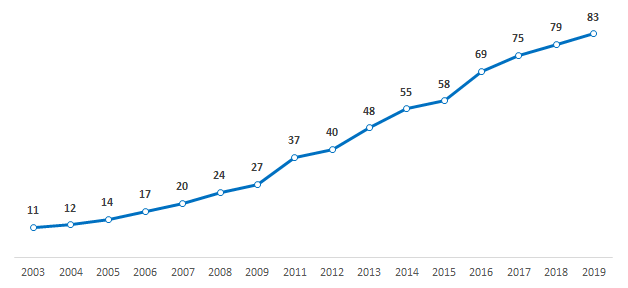
\includegraphics[width=1.0\linewidth]{../../../imagens/acesso-internet.png}
                \caption{Evolução do percentual de domicílios com acesso para internet (Fonte: SIDRA 2016-2019  (apud Schmitz et al., 2021).}
                \label{dc69b8cf40fae2ba00158e43d2db2d294110957c}
\end{minipage}%
\hspace{0.5cm}
\end{figure}



As novas gerações precisam saber que não foi sempre assim. Muito embora a percepção corrente de que o uso de computadores e celulares é indispensável para o convívio na sociedade, a rigor seu uso é relativamente recente.

É possível identificar a evolução das telecomunicações, a partir do século passado, como origem das transformações tecnológicas e digitais disponibilizadas em larga escala. Pierre Levy, no livro "Cibercultura"(LEVY,2000):


\noindent\begin{center}\mbox{\centering\fbox{\centering\par\parbox{0.7\linewidth}{\small\textit{"Durante uma entrevista nos anos 50, Albert Einstein (1879-1955) declarou que três grandes bombas haviam  explodido durante o século XX: a bomba demográfica, a bomba atômica e a bomba das telecomunicações. Aquilo que Einstein chamou de bomba das telecomunicações foi chamado, por meu amigo Roy Ascott (um dos pioneiros e principais teóricos da arte em rede), de segundo dilúvio, o das informações. As telecomunicações geram esse novo dilúvio por conta da natureza exponencial, explosiva e caótica de seu crescimento. A quantidade bruta de dados disponíveis se multiplica e se acelera. A densidade dos links entre as informações aumenta vertiginosamente nos bancos de dados, nos hipertextos  e nas redes. Os contatos transversais entre os indivíduos proliferam de forma anárquica. É o  transbordamento caótico das informações, inundação de dados".}\normalsize}}}\end{center}


Ainda, segundo Pierre Levy,


\noindent\begin{center}\mbox{\centering\fbox{\centering\par\parbox{0.7\linewidth}{\small\textit{"O segundo dilúvio não terá fim. Não há nenhum fundo sólido sob o oceano de informações. Devemos aceitá-lo como nossa nova condição. Temos que ensinar nossos filhos a nadar, a flutuar, talvez a navegar."}\normalsize}}}\end{center}


Para a sociedade chegar nesse ponto, os governos e a iniciativa privada tiveram que, continuamente, investir no desenvolvimento de inovações científicas e tecnológicas, provendo a infraestrutura de comunicações e de redes digitais, bem como os meios de acesso a essas redes. O esforço científico e tecnológico de pós-guerra americano, liderado por Vannevar Bush a partir do relatório " Science-The endless frontier" (5 de julho de 1945), foi o motivador da criação do National Science Foundation, em 1950; e pode ser considerado  o ponto de partida para o protagonismo do Estado no investimento em inovações tecnológicas, na segunda metade do século XX.

Em outra ponta, os governos tiveram que formular políticas públicas para disponibilizar e preparar os cidadãos para que pudessem se apropriar dessas tecnologias.

A partir da segunda metade do século XX, as redes digitais estavam vinculadas à academia, às instituições de pesquisa e área de defesa (ARPANET,2022), num contexto de coordenação estatal.

No início da última década do século XX, essas inovações  foram avançando em direção ao suprimento das necessidades de relacionamento do cidadão com o governo. Após esse período, os serviços baseados nestas inovações foram mais longe e alcançaram  os demais aspectos dos indivíduos; inclusive na sua relação com os prestadores de serviços privados.

Essa expansão ocorreu como resultado de várias ações e a sua universalização é consequência do surgimento de novas formas de relacionamento social, viabilizadas pelas redes digitais, que tornaram mais acessíveis novas ferramentas.

Tais transformações tiveram impactos econômicos e sociais profundos, inclusive nas relações de trabalho, tanto na criação e extinção de postos de trabalho,  quanto em suas formas de contratação, jornada e remuneração; acarretando a precarização dos direitos trabalhistas. Essas mudanças estão bem descritas  no relatório da Unesco,  de 2004 "Social Transformation in an Information Society: Rethinking Access to You and the World" (DUTTON, 2004).

A amplitude destas transformações foi sintetizada no conceito de "Sociedade da Informação", às vezes, referido como "Era Digital" ou "Era da Informação".

O efeito dessas transformações no mundo do trabalho exige dos governos, das empresas e dos cidadãos uma constante e rápida readaptação  nas relações de produção, de novos saberes, e de  competências. Também o sistema educacional vem sendo desafiado a se adaptar, uma vez que é dele que se espera o preparo dos cidadãos para a nova realidade.

Inicialmente essas mudanças eram associadas à substituição do trabalho humano decorrente da automação industrial. Mas a radicalização no uso de soluções digitais, inclusive de inteligência artificial, associadas ao aumento da conectividade, vêm substituindo, segundo (Manyika (2016), "capacidades cognitivas que antes eram exclusivas de humanos". Uma das consequências mais radicais é o surgimento de novos meios de exploração humana, representados pela "Gigs Economy" (Manyika,2016) ou "Economia do Bico", que precariza as relações trabalhistas por meio de plataformas, que as impessoaliza a ponto de camuflar a exploração. O termo "bico" aqui está sendo usado como tradução livre de "gigs", que nos Estados Unidos é uma gíria usada para trabalho temporário. A uberização é um exemplo de relação de trabalho no contexto da Gigs Economy.

Vários países têm buscado uma melhor preparação para enfrentar essas transformações. Para isso, têm procurado remodelar seus sistemas educacionais, uma vez que um eventual atraso em relação aos demais países pode afetar a prosperidade (CONGRESS,1998) de suas populações, sua autonomia e liberdade.

Mais do que "treinar" os cidadãos, quanto ao uso  de serviços digitais, a educação tem um papel fundamental de prepará-los para a sua inserção autônoma e digna na sociedade, transformada pelas tecnologias de informação e comunicação. Portanto, o desafio do Estado não se limita a estabelecer políticas públicas de provimento de infraestrutura para que o cidadão possa ter acesso e se beneficiar dos recursos digitais e de comunicação, mas, principalmente, preparar estes cidadãos para que contribuam com a construção desses recursos, beneficiando-se da autonomia e prosperidade, que  essa construção gera.

O cidadão, também, precisa ser capaz de entender "o que está por trás" desses sistemas digitais, para que possa reagir aos excessos da "algoritmização" de suas relações com outros indivíduos.

Assim, antecipando  uma das conclusões desta dissertação, é no contexto do "segundo dilúvio" de Ascott que se insere a necessidade de um programa educacional como o WASH.

A percepção da importância da educação para a prosperidade da sociedade não é novidade. No caso americano, por exemplo, remonta aos primórdios de sua independência. Em termos globais, é possível perceber o reconhecimento de sua importância desde a Grécia e do Egito antigos.

No capítulo "Fundamentação Teórica," revisaremos as origens do conceito de "Science, Technology, Engineering and Mathematics" (STEM), mostrando que em 1790, o presidente George Washington, em seu primeiro discurso do "Estado da União", enaltecia a ciência e a literatura como  basilares para a "felicidade pública" (Relatório CRS para o Congresso, www.crs.gov, 2012). Essa percepção de valor da ciência e da cultura perdura até os dias atuais. Em muitos momentos foi estimulada, inclusive, como resposta às ameaças externas, como foi o caso da mobilização americana para fazer frente ao sucesso soviético no programa espacial, representado pelo pioneirismo do lançamento do satélite Sputnik, no final da década de 50. É no cenário da Guerra Fria, que a política de educação em STEM e alfabetização científica e tecnológica passaram a ser vistas mais claramente como um bem comum, mesmo muito antes do uso desse acrônimo de forma oficial.

Não obstante esta permanente percepção pública da importância e do valor da ciência, os Estados Unidos não conseguiram manter uma formação de qualidade nas áreas STEM.

Nos anos 90, os EUA identificaram fragilidades na educação STEM com prejuízo ao "poderio bélico e tecnológico nacional", à inserção de seus cidadãos no novo mundo do trabalho, de forma autônoma, soberana  e próspera. Essas fragilidades foram, relativamente evidenciadas pelo baixo desempenho de adolescentes americanos no "Programme for International Student Assessment" (PISA)  (CATTERALL,2017). Com isso, o governo americano teve que propor ações para atualizar as competências curriculares, visando manter uma inserção hegemônica na economia do século XXI.

Segundo o Relatório "Congress Research Service" (CRS-Serviço de pesquisa do Congresso Americano), mais de 200 projetos de Lei contendo o termo "educação científica" foram apresentados entre o período de 1987 a 2008. O mesmo relatório aponta que 13 agências federais estavam envolvidas em programas ou atividades de educação "STEM". (Pag.2 do Relatório).

Os atores governamentais e estudiosos daquele período identificaram que faltava aos EUA uma política nacional, uniforme e inclusiva de ensino de ciências, pois era possível categorizar diferentes ênfases sobre o assunto no vasto sistema educacional americano (CATTERALL, 2017).

Mas, existia também, o reconhecido pioneirismo da comunidade acadêmica americana nos métodos voltados ao aprendizado de temas relacionados ao STEM, ainda que não identificados sob esse acrônimo ou mesmo que não amplamente disseminados em seu sistema educacional, como viriam a reconhecer os Relatórios do Congresso Americano (CONGRESS, 1998).

Seymour Papert, matemático sul-africano, radicado nos EUA, do Laboratório de Inteligência Artificial do Massachusetts Institute of Technology (MIT), foi um  cientista e educador que acreditava  no  uso do computador como forma de revolucionar o sistema  educacional,  desde os anos 60.

Papert foi um cientista visionário, ao pensar a aprendizagem de crianças de forma diferente. Em 1968, escreveu o artigo, " Teaching Children Thinking "  em que abordava  o tema sobre crianças, educação e computadores. No capítulo de Fundamentação Teórica, sua contribuição será aprofundada, mas é necessário antecipar, aqui, alguns elementos para que seja possível delimitar o escopo da presente pesquisa.

Cabe reconhecer, de forma resumida, que, quando Papert formulou suas ideias, nos anos 70, os computadores ainda não eram amplamente acessíveis ou disponíveis para uso doméstico. Naquele tempo, no existia conceito de "microcomputadores". Equipamentos com poder de processamento milhares de vezes inferior ao de um notebook ocupavam centenas de metros quadrados (CIPOLI, 2012). Segundo (SOLOMON et al. (2020), "em 1966, os computadores eram poucos, grandes e espalhados", os custos eram muito altos e o acesso era muito restrito.

Mas, mesmo na forma de mainframes centralizados (computadores de grande porte) com as limitações indicadas acima, foi possível a Papert realizar incursões desbravadoras no campo da aprendizagem para crianças utilizando computadores, ainda que sem uma ampla disseminação no sistema educacional americano.

Uma geração de educadores foi formada em torno das ideias de Papert, para quem a prática de programação de computadores, no ensino fundamental, poderia ter um papel importante no aprendizado de muitas disciplinas, tais como matemática, ciências e linguagem. A proposta de Papert, até por enfatizar o aprendizado de crianças, não tinha qualquer ambição de capacitação profissional e, por si só, não visava diretamente fazer frente aos desafios do "mundo do trabalho", que foram sendo introduzidos pelas transformações inerentes à Sociedade da Informação, nas décadas subsequentes. Para Papert o uso do computador poderia funcionar como indutor da aprendizagem de um amplo espectro de disciplinas.

Diferentemente de um simples treinamento para usar computadores, o método de Papert representava uma mudança em paradigmas educacionais, focalizando a aprendizagem em detrimento do ensino  (NEGROPONTE,2004). A ideia era " aprender o que se precisa" e não "aprender o que se deve ".

O caráter estritamente educacional e a peculiar abordagem das propostas de Papert são apontados em "Brazil Plan" (NEGROPONTE, 2004), embora muito a posteriori por seus colegas, como uma alternativa para a inserção do indivíduo na "era digital" (digital age).

Assumindo que o conceito de "era digital" se refere às transformações tecnológicas que viabilizaram a "Sociedade da Informação",  é razoável depreender, a partir do que está presente em Brazil Plan  (NEGROPONTE, 2004), que seus sucessores no MIT, de forma independente, entendiam a proposta de Papert como um caminho natural para a melhor inserção dos indivíduos na Sociedade da Informação.

O pioneirismo de Papert permite reconhecer nele uma inspiração para as demais iniciativas educacionais no estilo STEM, que vieram depois. Essas iniciativas propunham uma educação despojada de formalismos, voltada para a resolução de problemas, ao invés da histórica obsessão por conteúdos. Esse tipo de abordagem inspirou boa parte dos conceitos subjacentes como "maker culture", entre outros.

As preocupações com o relativo baixo desempenho em  educação STEM, que se aprofundavam nos EUA, nos anos 90, alcançaram o resto do mundo. Começaram a surgir propostas para tentar promover a qualificação da educação em países em desenvolvimento, por meio do uso intensivo de computadores, nos moldes do que enxergara Papert em seus trabalhos seminais.

Dentre estas propostas, destaca-se o "One Laptop per Child-OLPC", projeto elaborado por pesquisadores do MIT  (NEGROPONTE, 2004), sucessores dos trabalhos de Papert. Uma descrição detalhada sobre as características e história do OLPC pode ser encontrada no capítulo de Resultados e Análises, bem como em outras referências (ALVAREZ, 2015); cabendo antecipar que o OLPC foi apresentado ao governo brasileiro, em 2005, durante o Fórum Econômico em Davos, como solução para os problemas educacionais brasileiros.

Podemos sintetizar que o OLPC envolvia a distribuição massiva de laptops (notebooks) para crianças e adolescentes dos ensinos fundamental e médio, com vistas a universalizar o acesso à internet, na escola pública brasileira.

Esta universalização visava oportunizar várias práticas pedagógicas da escola pública, dentre elas a programação de computadores, consequência direta do pensamento de Papert. Para que pudesse ser implementada nos prazos e formato pretendidos pelo MIT, a proposta do OLPC comprometeria boa parcela do orçamento do Ministério da Educação na compra de laptops (notebooks). Foi esse comprometimento, e o risco a ele associado, que estimularam o Governo Brasileiro a buscar formas de avaliar sua efetividade. Segundo a avaliação do CTI Renato Archer, do Projeto OLPC  (MAMMANA, 2006), solicitada pela Presidência da República, a proposta do MIT tinha foco na distribuição de equipamentos para estudantes, sem uma visão estruturada de como as pessoas do sistema educacional brasileiro se apropriariam dessa tecnologia.

A avaliação do Projeto OLPC proporcionou uma ressignificação para a proposta, permitindo compreender mais profundamente os desafios do uso intensivo de Tecnologia da Informação e Comunicação (TIC), no contexto da escola pública brasileira e, com isso, propor uma alternativa.

O Programa WASH nasceu como uma proposta alternativa ao OLPC (MAMMANA e TOZZI, 2018), com custo inferior, que não exigia a aquisição de milhões de equipamentos, mas que se inspirava nos mesmos conceitos exitosos de Papert, que fundamentaram a proposta do OLPC.

Cabe uma breve descrição nesta introdução sobre o Programa WASH, ressalvando-se que o aprofundamento constará no capítulo de Resultados e Análise. O WASH busca criar espaços de interação, na forma de  vivências, oficinas praticadas no ambiente da escola básica, que visam a promoção dos valores do método científico. A ênfase são atividades relacionadas ao STEM e, posteriormente STEAM, que inclui a arte na lista das disciplinas, como tantos outros autores fizeram no início do século (CATTERALL, 2017) (MAMMANA e TOZZI, 2018)  (YAKMAN, 2019). Desta forma, um novo acrônimo surgiu agregando Science, Technology Engineering, Arts and Mathematics, o STEAM (YAKMAN, 2019).

Destarte, de forma sintética, pode-se antecipar que o WASH realiza atividades STEAM no turno e contraturno da escola básica, desvinculadas do currículo da escola formal, cujos valores principais se alicerçam no método científico. O WASH não é um curso, mas se constitui em espaços de interação humana para experimentação e convivência entre indivíduos, no contexto do desenvolvimento de projetos de vários níveis de complexidade.

Pela forma como os pilotos do WASH, em anos iniciais, acabaram sendo implementados no  CTI Renato Archer, houve a consolidação da visão e da prática vivenciada de que instituições, unidades de pesquisa poderiam estabelecer as pontes entre centros de excelência de pesquisa, educação a partir do ensino básico e a comunidade. Em particular, a existência de um convênio entre o CTI Renato Archer e o Instituto Federal de Educação, Ciência e Tecnologia de São Paulo (IFSP), campus Campinas, no momento da fundação do WASH, em 2013-2014, permitiu experimentar o papel que uma universidade poderia ter no Programa. Esta experiência inicial configurou a conceituação do WASH, que perdura até os tempos atuais- dez anos depois, com intensa participação dos campi do IFSP e do IFPR na ampliação regional, estadual e interestadual.

O Programa WASH tem seu método descrito no Documento de Referência, anexo à Portaria CTI 178/2018 (ver Fig. 2), que estabelece uma "liturgia do seu fazer" (CNPq, 2020) para realizar oficinas, bem como os papéis de cada participante e sua forma de operação. Mas, é evidente que, por ser longevo, alcançando em 2023 a marca de 10 anos, o WASH passou por muitas transformações em relação à proposta inicial, requerendo uma constante caracterização e revisão, com base em indicadores e análise de seus processos.



\captionsetup{format=plain}
\begin{figure}[htb]

	\begin{center}

		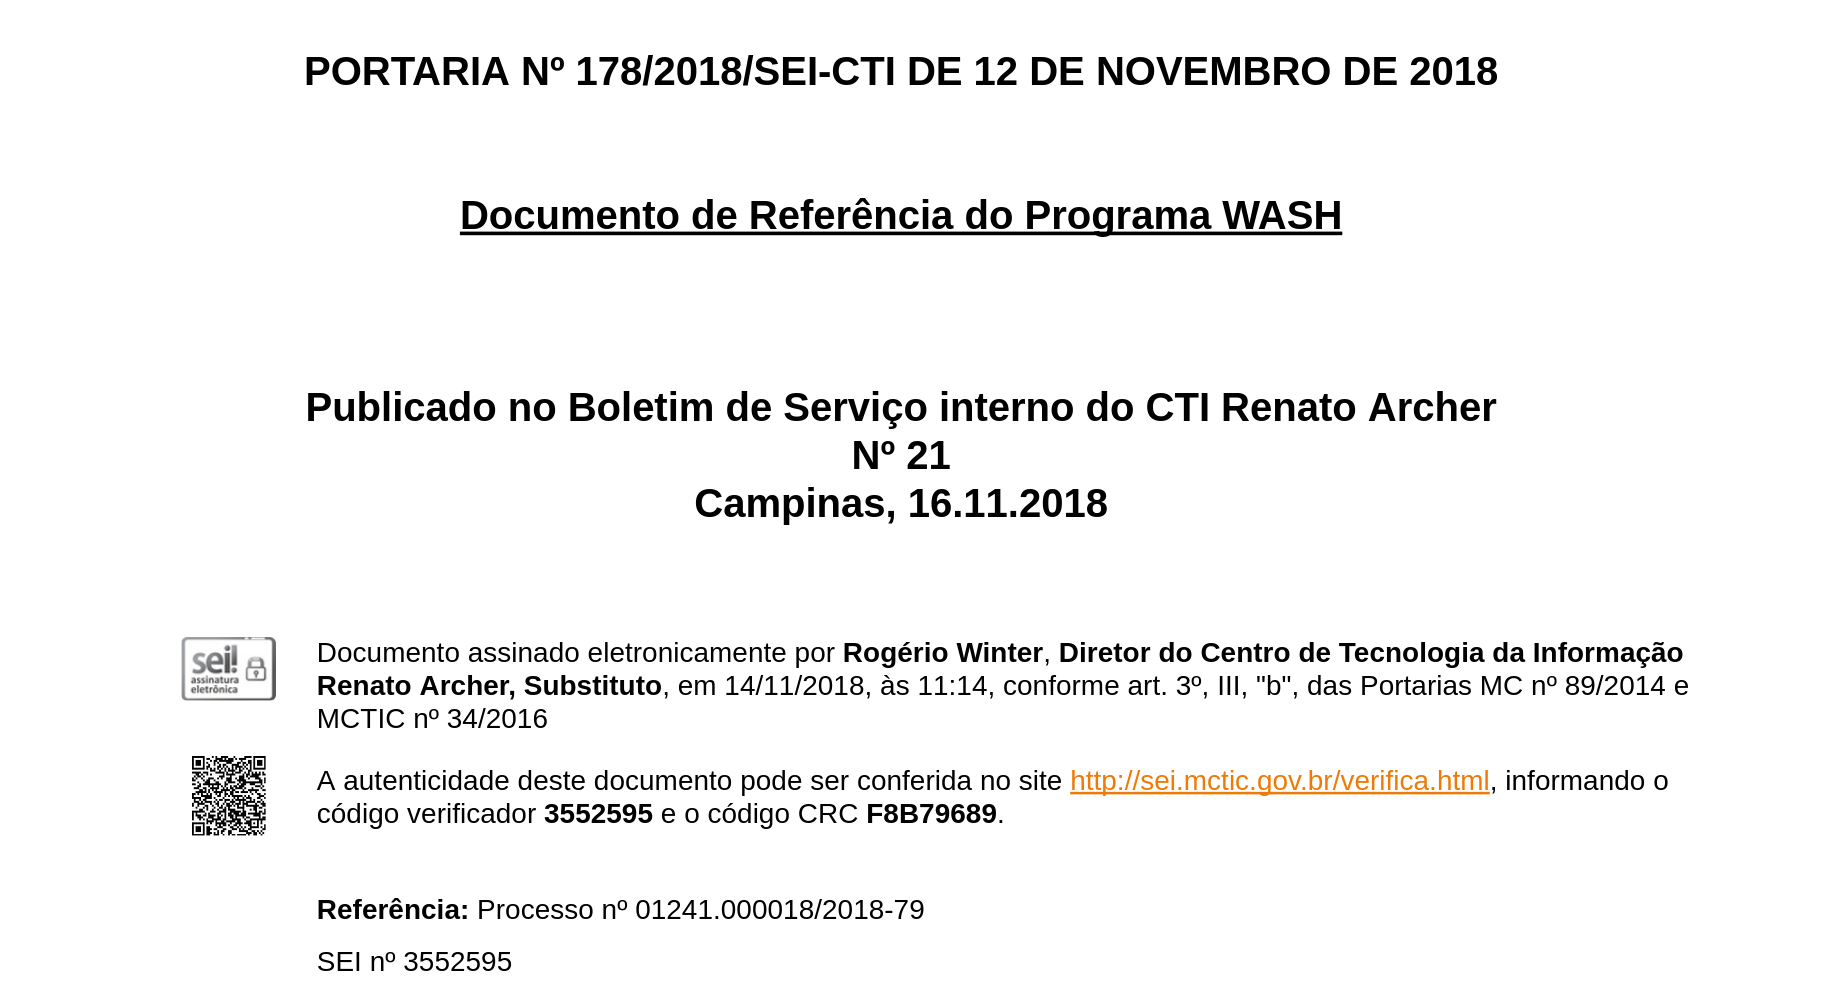
\includegraphics[max size={\textwidth}{\textheight}]{../../../imagens/capa-portaria-178.png}

	\end{center}

	\caption{\label{5369350fe31df6a16c506eebf158a3d2b77020ea}@[caption-5369350fe31df6a16c506eebf158a3d2b77020ea]@}

\end{figure}

Por curioso, não obstante os criadores do WASH tenham se inspirado nos conceitos pedagógicos do OLPC, também opuseram-se à aquisição dos notebooks (MAMMANA e TOZZI, 2018) pelo governo brasileiro, em razão de outros aspectos do projeto que se mostravam inviáveis, nos campos orçamentário, industrial, ergonômico, inclusivo e de logística (MAMMANA,2005).

Neste trabalho, serão abordadas a história e a caracterização do Programa WASH. O documento fundamental a ser usado para permitir a caracterização do WASH é a própria Portaria CTI 178, cujo anexo é o Documento de Referência do WASH, além de outros registros, tais como planos de trabalho, publicações, relatórios,  produção audiovisual etc.  A análise do Documento do WASH permitirá compreender "o que o WASH gostaria de ter sido", ao passo que todo o desenvolvimento do trabalho buscará estabelecer "o que o WASH de fato conseguiu ser". A partir desses dois entendimentos, será proposta uma revisão do Documento de Referência, com vistas a aprimorá-lo.

A abordagem adotada na presente dissertação se encaixa no método de "Estudo de Caso"  e buscará contar, por meio da aplicação de um método historiográfico, toda essa trajetória que se inicia no que foi descrito aqui, bem como identificar o método do Programa WASH e seus resultados.

\section[WASH: projeto, programa, sistema, organização ou política pública?]{WASH: projeto, programa, sistema, organização ou política pública?}\label{WASH: projeto, programa, sistema, organização ou política pública?}
É oportuno que se busque, logo no início desse estudo, uma uniformização na denominação do WASH. Trata-se de um projeto, de um programa, de um sistema, de uma organização ou de uma protopolítica pública?

Para responder a essa pergunta é preciso, adiantar que o WASH como Programa de educação científica e tecnológica, ocorre nas escolas, oferece a linguagem de programação de computador e a iniciação científica a partir do  ensino médio, junto ao Conselho Nacional de Desenvolvimento Científico e Tecnológico CNPq. As emendas parlamentares financiam as bolsas,(ver  lista de emendas na seção 4.2.1).

Por essa razão, historicamente, temos nos referido ao WASH como projeto, mas, talvez, não seja a melhor forma de denominá-lo.

Os planos de trabalho do WASH são registrados no CNPq e especificam como será a execução das emendas parlamentares. Os quais estão organizados da seguinte forma:


\begin{itemize}
\item título do projeto;
\item introdução, materiais e métodos;
\item objeto, objetivo e público alvo;
\item prazo de execução e entregáveis;
\item identificação da equipe;
\item cronograma e
\item orçamento
\end{itemize}

Os planos de trabalho podem ser complementados por aditivos, prorrogação de prazo e vigência; mas, em geral, essas alterações não podem ampliar seus escopos de execução.

Iniciado, em 2013, sem financiamento, o WASH recebeu, de 2016 até o 2022, quinze emendas parlamentares, cada uma com seu plano de trabalho específico, submetido ao CNPq e registrado na Plataforma Carlos Chagas, (CHAGAS, 2022).

Esses planos de trabalho, embora com características e escopos específicos, seguiram diretrizes de execução que têm em comum a promoção da aprendizagem STEAM.

Portanto, essa repetição de projetos sequenciais, cada um com sua especifidade, mas todos seguindo a mesma diretriz, indica que o WASH tem características de Programa, como é possível verificar nos conceitos do Project Management Institute  (PMI,2008), citadas por  (Weaver, 2010):


\noindent\begin{center}\mbox{\centering\fbox{\centering\par\parbox{0.7\linewidth}{\small\textit{Programas focalizam a coordenação de um conjunto de projetos relacionados, bem como de outras atividades, ao longo do tempo, para entregar benefícios para a organização (Tradução livre de apud.(PMI, 2008).}\normalsize}}}\end{center}


Desta forma, é razoável aceitar que aquilo que vem sendo chamado de Projeto WASH já possa ser considerado como Programa, dado que é justamente um conjunto de projetos, com atividades coordenadas e com métodos que, embora evoluam no tempo, seguem uma diretriz.

Não obstante ser possível atribuir tacitamente ao WASH uma característica de programa, em termos dos citados conceitos do Project Management Institute (PMI), há mais elementos para se considerar.

A vinculação do WASH ao governo federal exige a observância de normas para a criação de programas, a exemplo da edição de atos de ofício (portarias, decretos etc) específicos para tal.

A ausência desses instrumentos legais, que estabeleceriam um "programa federal", indica que a sobrevivência do WASH depende da aprovação, a cada nova emenda parlamentar, das propostas de plano de trabalho apresentadas ao CNPq. Em outras palavras, a existência do WASH depende da diligência da equipe na busca constante por recursos financeiros (emendas), bem como da avaliação anual, por parte do CNPq e parlamentares, dos resultados alcançados, não havendo a garantia de continuidade que um programa proveria.

Essa característica exige um cuidado com o uso da palavra "programa", sendo necessário esclarecer o contexto em que pode ser usada, como segue: o WASH efetivamente praticado extrapola os limites de qualquer um dos planos de trabalho, que o implementaram desde sua criação até os dias de hoje.

Por outro lado, veremos, ao longo desta dissertação, que também é possível entender o WASH como um sistema, sob a ótica de uma da definição a seguir:


\noindent\begin{center}\mbox{\centering\fbox{\centering\par\parbox{0.7\linewidth}{\small\textit{"(Sistema é um) conjunto de elementos, concretos ou abstratos, intelectualmente organizados." (fonte: Oxford Languages através do Google)}\normalsize}}}\end{center}


A definição de sistema trazida por (BERTALANFFY, 1968) também, corrobora com esse entendimento:


\noindent\begin{center}\mbox{\centering\fbox{\centering\par\parbox{0.7\linewidth}{\small\textit{"Sistema é um complexo de elementos interagentes que é aberto para o ambiente e interage com ele" (Fonte:  (BERTALANFFY, 1968), tradução livre)}\normalsize}}}\end{center}


A importância de considerar o WASH como um sistema tem a ver com aplicação de métodos de análise de sistemas, a exemplo da modelagem de dados relacional para a criação de sua plataforma de gestão, a "Platuóxe".

Quanto a verificar se o WASH é uma organização, podemos usar a seguinte definição (MAXIMIANO, 1981):


\noindent\begin{center}\mbox{\centering\fbox{\centering\par\parbox{0.7\linewidth}{\small\textit{"As organizações são grupos sociais deliberadamente orientados para a realização de objetivos ou finalidades (...)" (Fonte: MAXIMIANO, 1981)}\normalsize}}}\end{center}


Usando palavras diferentes, o mesmo autor nos contempla com outra forma de definição que é particularmente interessante para o WASH:


\noindent\begin{center}\mbox{\centering\fbox{\centering\par\parbox{0.7\linewidth}{\small\textit{"(...) uma organização é uma combinação de esforços individuais que tem por finalidade realizar propósitos coletivos. Por meio da organização torna-se possível perseguir e alcançar objetivos que seriam inatingíveis para uma pessoa." (Fonte: MAXIMIANO, 1981)}\normalsize}}}\end{center}


As definições de Maximiano indicam a possibilidade de qualificar o WASH também, como organização, dado que ele é constituído por um grupo de pessoas que conjuminam esforços individuais para alcançar propósitos coletivos. Essa possibilidade dá a abertura para empregar, em nosso estudo, o método historiográfico aplicado à administração pública, como se verá em Materiais e Métodos.

O WASH também pode ser considerado uma protopolítica pública, daquelas que são vivenciadas mas que ainda não estão formalizadas numa lei federal. Essa possibilidade de entendimento surge de vários elementos, entre eles, adoção ao método do WASH, a existência de leis municipais que criaram o Programa WASH nas cidades de Prado Ferreira e Dr. Camargo, ambas no Paraná; ou de normas infralegais para a mesma finalidade nas cidades de Jacareí (SP)e Santo Inácio (PR), entre outras. Essas experiências locais servem de piloto para uma possível legislação federal, que venha a transformar o WASH em uma política pública de fato.

Considerando essas delimitações conceituais, decidimos adotar, na maior parte das vezes, o epíteto "Programa" para qualificar o WASH, sem prejuízo para as demais dimensões (sistema, organização e protopolítica pública).

Assim, reconhecemos antecipadamente que o WASH tem, as dimensões de programa, sistema, organização e protopolítica, o que será demonstrado ao longo do estudo.

\section[Objeto]{Objeto}\label{Objeto}
Este trabalho tem por objeto de estudo a história e a caracterização, do Programa WASH considerando o período de novembro de 2013 a outubro de 2022.

\section[Objetivos]{Objetivos}\label{Objetivos}
Essa dissertação tem objetivos  "Gerais" e "Específicos".

\subsection[Objetivo Geral]{Objetivo Geral}\label{Objetivo Geral}
Estudar e caracterizar o Programa WASH em dois eixos:(1) sua história e (2) seus indicadores.

\subsection[Objetivos Específicos]{Objetivos Específicos}\label{Objetivos Específicos}



\begin{itemize}
\item identificar no Documento de Referência (Portaria CTI 178/2018) os pontos que requerem adequação às contínuas mudanças sociais e educacionais do país, que ocorreram depois da sua edição;
\item verificar se os objetivos presentes nesse documento se concretizaram, através da validação das hipóteses levantadas nesta dissertação;
\item identificar as práticas do WASH que precisam ser melhoradas;
\item identificar novos conceitos e práticas que precisam ser incorporados ao WASH; e
\item produzir uma revisão do Documento de Referência do WASH como produto educacional a ser apresentado ao final desta pesquisa.
\end{itemize}

\section[Hipóteses]{Hipóteses}\label{Hipóteses}
Decidimos utilizar como origem das hipóteses deste estudo parte dos objetivos presentes na Portaria 178/2018. Assim, podemos dizer que, ao validar uma hipótese com essa origem, estamos verificando se aquele objetivo foi alcançado pelo Programa WASH.

Complementarmente aos objetivos da Portaria CTI 178/2018, enunciamos hipóteses adicionais, com base em nossa vivência como partícipes do Programa. As hipóteses obtidas, a partir dessas duas origens, foram organizadas em uma lista mostrada adiante.

O trabalho de verificação das hipóteses é imprescindível para conhecer a eficiência e eficácia do WASH,como Programa de educação.

O fato de um objetivo estar declarado no Documento de Referência da Portaria CTI 178/2018 não significa que o mesmo foi alcançado. Neste sentido, esses objetivos, base das hipóteses, refletem " o que o WASH gostaria de ter sido ". Ao passo que, nesta dissertação, verificaremos hipótese a hipótese, " o que o WASH conseguiu ser ". As falhas eventualmente encontradas contribuirão para apontar o caminho que deve ser seguido na revisão do Documento de Referência.

\subsection[Hipótese 1: Eficiência e Eficácia do WASH]{Hipótese 1: Eficiência e Eficácia do WASH}\label{Hipótese 1: Eficiência e Eficácia do WASH}
O enunciado é:


\noindent\begin{center}\mbox{\centering\fbox{\centering\par\parbox{0.7\linewidth}{\small\textit{Hipótese 1: O WASH conseguiu promover a disseminação de conhecimentos em Ciência e Tecnologia, beneficiando milhares de pessoas em dezenas de cidades pela oferta de oficinas de curta duração nos ensinos fundamental, médio e superior.}\normalsize}}}\end{center}


O enunciado acima pode ser verificado pela avaliação da eficiência e eficácia do WASH, no contexto do eixo 2-indicadores.

\subsection[Hipótese 2: Orientação a Projetos]{Hipótese 2: Orientação a Projetos}\label{Hipótese 2: Orientação a Projetos}
O enunciado é:


\noindent\begin{center}\mbox{\centering\fbox{\centering\par\parbox{0.7\linewidth}{\small\textit{Hipótese 2: O WASH estimula a aprendizagem por meio da orientação a projetos para alunos dos ensinos médio e técnico e graduação em temas relacionados ao STEAM.}\normalsize}}}\end{center}


\subsection[Hipótese 3: Origem do WASH]{Hipótese 3: Origem do WASH}\label{Hipótese 3: Origem do WASH}
O enunciado é:


\noindent\begin{center}\mbox{\centering\fbox{\centering\par\parbox{0.7\linewidth}{\small\textit{Hipótese 3: O WASH teve como origem: (i)  o aprendizado com a avaliação do OLPC (NEGROPONTE, 2004) pelo governo brasileiro; (ii) as práticas do Programa Governo Eletrônico de Serviço de Atendimento ao Cidadão (GESAC); e (iii) a Avaliação do Programa de Inclusão Digital (PID) da Secretaria de Inclusão Social (SECIS), do Ministério da Ciência e Tecnologia (CGEE, 2009).}\normalsize}}}\end{center}


\subsection[Hipótese 4: Prática Pedagógica do WASH]{Hipótese 4: Prática Pedagógica do WASH}\label{Hipótese 4: Prática Pedagógica do WASH}
O enunciado é:


\noindent\begin{center}\mbox{\centering\fbox{\centering\par\parbox{0.7\linewidth}{\small\textit{Hipótese 4: O WASH se inspira em conceitos e práticas de Seymour Papert (PAPERT, 1980), combinados com outros métodos, tendo se embasado, em parte, nas experiências pioneiras da Profa. Dra. Afira Vianna Ripper, na transposição dos conceitos de Papert para o Brasil e no trabalho de iniciação científica para o ensino fundamental.}\normalsize}}}\end{center}


\subsection[Hipótese 5:WASH como proto-política pública]{Hipótese 5:WASH como proto-política pública}\label{Hipótese 5:WASH como proto-política pública}
O enunciado é:


\noindent\begin{center}\mbox{\centering\fbox{\centering\par\parbox{0.7\linewidth}{\small\textit{Hipótese 5: O WASH pode ser considerado como uma protopolítica pública nacional, apesar da Portaria CTI 178/2018 não se constituir em um instrumento de criação desse tipo de política.}\normalsize}}}\end{center}


\subsection[Hipótese 6: WASH como organização heterárquica]{Hipótese 6: WASH como organização heterárquica}\label{Hipótese 6: WASH como organização heterárquica}
O enunciado é:


\noindent\begin{center}\mbox{\centering\fbox{\centering\par\parbox{0.7\linewidth}{\small\textit{Hipótese 6: Em termos organizacionais, o WASH é estruturado através de relações heterárquicas.}\normalsize}}}\end{center}


\section[Problema]{Problema}\label{Problema}
Com a passagem dos anos, os desafios do Programa WASH foram se transformando. Práticas tiveram que ser adaptadas e outras incorporadas.

Um exemplo eloquente de transformação de realidade, que requeriu revisão de práticas do WASH, decorreu da pandemia de COVID-19, que exigiu o isolamento social, inviabilizando vivências presenciais.

O Programa WASH que se restringia as atividades presenciais, precisou criar formas de praticar oficinas remotamente, o que contrariava as diretrizes que estabeleciam a realização exclusivamente presencial. Assim, como em todo o sistema escolar, essa imposição exigiu vencer barreiras técnicas de conectividade e conceituais com relação às atividades remotas. Esta transformação de prática ainda não está refletida nas diretrizes presentes na Portaria CTI 178/2018.

Outros desafios contemporâneos podem ser citados, como a promulgação da Lei Geral de Proteção de Dados (LGPD), a incorporação do registro de nome social, as transformações tecnológicas nas ferramentas de programação pedagógica, entre outros. O Documento de Referência anexado à Portaria CTI 178/2018 ,também, não trata esses aspectos.

A verificação ou não das hipóteses elencadas na seção anterior, poderá contribuir para a identificação de outros problemas.

Isto posto, podemos sintetizar a situação-problema, através da seguinte pergunta: "Quais alterações devem ser realizadas no Documento de Referência do WASH para que o Programa possa evoluir e se adaptar às novas realidades?"

\section[Justificativa]{Justificativa}\label{Justificativa}
A aceitação do método do Programa WASH pelas instituições parceiras espalhadas pelos estados de São Paulo e Paraná, documentada por dezenas de instrumentos legais de adesão (portarias, boletins, entre outros - ver seção 4.2.2), permite vislumbrar a transformação do WASH em política pública. Acreditamos que há um potencial de crescimento nas adesões ao Programa, como resultado de uma almejada melhoria em suas práticas.

Portanto um próximo passo, necessário para que o Programa atinja o estágio de política pública consolidada (mas não suficiente) é realizar uma revisão em seu Documento de Referência, contido no anexo à Portaria CTI 178/2018, para que os problemas identificados na seção anterior, entre outros, possam ser equacionados.

Alcançado esse objetivo de revisão, outros passos de caráter de governo, que fogem ao escopo desse trabalho, serão necessários.

\chapter[FUNDAMENTAÇÃO TEÓRICA]{FUNDAMENTAÇÃO TEÓRICA}\label{FUNDAMENTAÇÃO TEÓRICA}
Neste capítulo,buscaremos a fundamentação para a vindoura escolha dos métodos, que serão efetivamente empregados para alcançar os objetivos deste estudo.

Assim, o presente capítulo, também, é dividido nos dois eixos principais da presente investigação:


\begin{itemize}
\item Eixo 1: história
\item Eixo 2: indicadores
\end{itemize}

Antes de prosseguir é necessário entender o papel do método em um trabalho científico. Essa compreensão pode ser construída pela análise da origem etmológica da palavra.


\noindent\begin{center}\mbox{\centering\fbox{\centering\par\parbox{0.7\linewidth}{\small\textit{"O étimo latino “methodus” é um dos fundamentos para a significação do termo “método”. Com o sentido de caminho (“chemin”, “route”), do grego odos (Clédat, 1914, 213), está presente em vários idiomas: “methode” (Al), “méthode” (Fr), “método” (Esp), “metodo” (It). Com o methodus e o seu significado mais abrangente, “caminho” (way, Weg, route, via e camino), designamos o nosso tipo ideal." (fonte: (FREITAS, 2019)}\normalsize}}}\end{center}


Tendo em vista a necessidade de escolher um caminho para chegar  aos objetivos desta pesquisa, serão descritos os fundamentos teóricos, que serão considerados para essa escolha de método.

Portanto, neste capítulo, não trataremos dos métodos efetivamente utilizados no trabalho, mas das opções que consideramos para escolher os métodos que de fato utilizamos.

É preciso declarar que temos sensibilidade aos argumentos apresentados por (GODOI et al, 2006), dando conta da impossibilidade " do método como corretor ou remédio, para as dificuldades "inerentes a uma inevitável insegurança epistemológica". Entretanto, não haverá como nos debruçarmos sobre isso com mais profundidade, havendo que prosseguir, mesmo que tão somente para, em caráter preliminar, "adquirir conhecimento de maneira instrumental", de uma busca por uma sempre questionável "objetividade científica" (GODOI et al.,2006), com a esperança de plantar uma semente para que outras abordagens possam se somar a nossa, contribuindo para a construção do conhecimento.

Uma característica da pesquisa bibliográfica, que apresentamos aqui, é seu  caráter instrumental, não voltado para gerar novos conhecimentos (interpretações) sobre a literatura em si.

Nosso objetivo principal é o de melhorar o Documento de Referência do Programa WASH e, para isso, decidimos otimizar nosso trabalho, usufruindo da colaboração de outros pesquisadores que já se debruçaram sobre os clássicos e  sintetizaram os métodos de nosso interesse.

Assim, nossa escolha bibliográfica sintetiza e consolida conhecimentos complementares que estão nos clássicos. Mas, fazemos isso sempre de forma crítica, para não nos apoiarmos em textos de baixa confiabilidade.

Essa forma dita "pragmática" de abordagem nos permite avançar no que realmente temos para contribuir, nos apoiando com segurança no trabalho de compilação e interpretação que outros já fizeram nas diversas áreas onde temos interesse. Além disso, nossa abordagem instrumental exige a exploração de referências mais recentes, porque essas acabam por compilar conhecimentos de várias áreas, apresentando descrições de métodos encapsuladas em formatos prontamente aplicáveis.

Finalmente, faz parte dessa fundamentação teórica uma revisão de alguns conceitos gerais, que permearão todo o texto, os quais estão presentes na última seção deste capítulo.

\section[Fundamentação: história (eixo 1)]{Fundamentação: história (eixo 1)}\label{Fundamentação: história (eixo 1)}
Para traçar a história e caracterizar o Programa WASH, o contexto no qual ele surgiu, quais políticas, projetos e ações, enfim, as diversas experiências que o antecederam (ver Hipóteses), faz-se  necessário que seja definido e aplicado o método. Mas, antes de defini-lo, revisitaremos conceitos pré-existentes que  desenvolveremos nesta seção.

Assim, nesta seção, complementada pelo Apêndice A, será revisitada a base teórica das práticas historiográficas, disponíveis para construir as narrativas sobre atividades e conceitos, que antecederam a existência do Programa WASH, a exemplo do GESAC, do OLPC e do Pensamento de Papert.



Ocorre que, pelo caráter recente de muitas das histórias que contribuíram para existência do WASH, elas ainda estão sendo contadas por diversos perspectivas e atores. Por ter sido testemunha ocular de algumas delas, esta autora tem a contribuir com sua própria narrativa, a qual não pode ficar restrita a uma simples crônica ou descrição de linha do tempo. Ao contrário, o eixo 1 foi desenvolvido de forma complementar ao eixo 2, estabelecendo uma abordagem plural, que deve culminar com a proposta de mudanças no Documento de Referência do WASH.

A nossa reconhecida proximidade com os fatos, que tentamos descrever e narrar nesta dissertação, exige um cuidado especial, porque, como alerta  (PIERANTI, 2022):


\noindent\begin{center}\mbox{\centering\fbox{\centering\par\parbox{0.7\linewidth}{\small\textit{(...) a perspectiva do autor está intrinsecamente ligada ao seu modo de ver e expor a História, sendo determinante, em parte, do seu relato e das interpretações daí decorrentes. (...) (fonte: (PIERANTI, 2022)}\normalsize}}}\end{center}


Esse risco não é novidade e pode-se dizer que foi abordado por Pierre Nora  (apud DOSSE, 2012), criador da ego-história, nos anos 80, quando o historiador assumia publicamente sua subjetividade. Considerando que, neste trabalho, estamos fazendo um tipo de "história do tempo presente"  (DOSSE, 2012), pelo caráter recente do período abordado, é indispensável "conhecer o lugar de enunciação do historiador, a instituição necessária em função da qual ele conduz sua investigação e o momento preciso durante o qual ele escreve a sua prática "  (DOSSE, 2012).

Esse reconhecimento de que se trata de uma história de tempo presente permite, de uma forma alternativa, considerar nosso trabalho, também, como um estudo de uma organização, onde o WASH assume essa dimensão, sem desconsiderar seu caráter de  programa, sistema ou protopolítica.

Assim sendo, não seria surpresa se alguém propusesse o emprego de métodos de administração, pertinentes à disciplina de "Organização, Sistemas de Métodos" (OSM) para estudar o WASH.


\noindent\begin{center}\mbox{\centering\fbox{\centering\par\parbox{0.7\linewidth}{\small\textit{Organização, Sistemas e Métodos é uma área da administração, que lida com um conjunto de técnicas, que têm como objetivo principal aperfeiçoar o funcionamento das organizações. (Fonte: (CARDOSO, 2014)}\normalsize}}}\end{center}


O WASH não pode ser considerado uma instituição dentro do Serviço Público Federal, porque carece de equipe estável ou documento formal de institucionalização, que defina um organograma ou outra forma de hierarquia, tão cara às corporações. Dentro da classificação de organizações oferecida por (MAXIMIANO, 1981), o WASH não se encaixa integralmente em "Grupos Sociais Secundários", que é justamente o grupo que tem características de institucionalização adequadas para o emprego da OSM.

Por esse motivo, concentraremos nosso trabalho nos dois eixos já elencados, sem o emprego da OSM.

Um outro aspecto a ser considerado é a posição da presente autora, que é partícipe do Programa/Organização, representado pelo WASH. A literatura nos socorre com a visão de que é impossível "negar a natureza humana do pesquisador e (...) seu conjunto de referências comuns ao tempo presente" (PIERANTI, 2022), mesmo quando o pesquisador está "distante da época e do local estudados". Reforça a confiança na possibilidade da autora produzir uma contribuição relevante para o  estudo, mesmo com um envolvimento próximo, a compreensão de que "deve prevalecer o reconhecimento das limitações da historiografia, implicando na aceitação dos resultados obtidos como um encaminhamento, dentre outros possíveis da pesquisa proposta" (PIERANTI, 2022).

(FAVERSANI, 1998) corrobora com esse entendimento, quando traz:


\noindent\begin{center}\mbox{\centering\fbox{\centering\par\parbox{0.7\linewidth}{\small\textit{O discurso científico, assim, não exige que se elimine a subjetividade do pesquisador, mas impõe que esta seja explícita em seus traços fundamentais, pressupondo que o cientista tenha que ter, necessariamente, clareza de quais as convicções que o movem quando realiza o seu trabalho, de quais idéias ele traz subjacentes quando exerce seu ofício que tem por função, entre outras coisas, criar elementos para a formação de opiniões em sua sociedade. (Fonte: FAVERSANI, 1998).}\normalsize}}}\end{center}


Também, conforta-nos a visão da epistemologia social que aponta para dois aspectos complementares, in verbis (GODOI et al., 2006) : "a questão da impossibilidade do distanciamento e da assepsia metodológica ao lançarmos olhares sobre o mundo; e o fato de que somos necessariamente parte daquilo que analisamos e, muitas vezes, tentamos modificar".

Ademais, desafia a nossa ambição de "encontrar um método", a compreensão de que a "historiografia não produziu um único método, mas diferentes tradições" (FIRAT, 1987).  Esse desafio se aprofunda, quando consideramos, por exemplo, (Costa e Silva, 2019), que apontam que a "pesquisa histórica ainda pode ser considerada marginal na maioria dos livros sobre metodologia de pesquisa em ciências sociais, pois não desfruta do espaço dado a outros métodos de pesquisa", in verbis. Lançando nossa ambição num limbo,  (Costa e Silva, 2019) reconhecem "que um dos argumentos mais fortes acerca dessa ausência (de descrição de método) transfere uma certa responsabilidade para o historiador, que não teria, por prática de pesquisa, de justificar metodologicamente o seu trabalho".

Para além de nos desafiar, muitas vezes, sentímo-nos arrefecidos em nosso intento de "encontrar um método" para o registro histórico, tendo em vista a negação de Popper em relação à cientificidade da história antiga, por exemplo (FAVERSANI, 1998), ou mesmo de sua utilidade (FIRAT, 1987).

Os historiadores vêm dando respostas a estes questionamentos, como no caso do exemplo citado por  (Costa e Silva, 2019), que relata a publicação, em 2013, pela revista "Management and Organizational History" ("Gestão e História Organizacional", em tradução livre), de uma edição especial entitulada "Doing Research in Management and Organizational Studies" (Fazendo pesquisa em gestão e em estudos organizacionais", em tradução livre). Esta edição especial é voltada para apresentar aplicações do método histórico, com orientações práticas (Costa e Silva, 2019) para o mundo dos estudos organizacionais. A mesma referência traz outros exemplos de iniciativas recentes semelhantes.

Dessa forma, não podemos nos deixar abater por essas questões epistemológicas, pelo menos do ponto de vista do trabalho historiográfico, que precisa ser realizado nesta dissertação, cabendo adotar uma visão pragmática para a questão, inspirada pelo entendimento de (FAVERSANI ,1998):


\noindent\begin{center}\mbox{\centering\fbox{\centering\par\parbox{0.7\linewidth}{\small\textit{Se assumimos uma postura científica, temos que o trabalho resultante sempre apresentará a seu leitor quais os caminhos que foram trilhados para obter determinados resultados, quais as  fontes foram utilizadas para se realizar este trabalho e quais os conceitos que servem de parâmetro para a leitura de fontes. Este rigor não é um mero capricho, mas uma rotina necessária para que este trabalho possa ser útil a outros pesquisadores, que se dedicam a pesquisas semelhantes, à medida que estes poderão, com estes elementos em mãos, extrair muito maior proveito para suas próprias reflexões. (Fonte: (FAVERSANI ,1998)}\normalsize}}}\end{center}


As busca pela verificação das Hipóteses indica uma complexidade que exige uma visão sistêmica entre abordagens históricas (eixo 1) e levamentamento estatístico de dados para a produção de indicadores (eixo 2). Esta menção a uma pluralidade de métodos e, em particular, a menção ao uso da estatística, nos motiva a olhar com mais cuidado para a segunda fase da Escola de Annales, quando se praticou a "História Quantitativa" (ver Apêndice A). Fazemos isso com o devido cuidado de não suscitar expectativas nos leitores que, depois, não conseguiremos satisfazer. Esse olhar, para a segunda fase da Escola de Annales, como referência para o nosso trabalho, será feito com a devida parcimônia e consciência do papel, limitado que podemos desempenhar em termos de historiografia.

Esta necessidade de uma visão sistêmica, que respeita os contextos presentes, é sustentada por vários autores e bem sintetizada em uma frase de (PIERANTI, 2022):


\noindent\begin{center}\mbox{\centering\fbox{\centering\par\parbox{0.7\linewidth}{\small\textit{"Análises descontextualizadas perdem sua relevância, na medida em que se tornam pouco factíveis ou possivelmente deslocadas da realidade" (PIERANTI, 2022)}\normalsize}}}\end{center}


Com isso em mente, no capítulo de Materiais e Métodos, tentaremos estabelecer um caminho próprio de historiografia, com inspiração na possibilidade de aplicar o método historiográfico como elemento de pesquisa em administração pública contemporânea, seguindo as opções indicadas em  (Costa e Silva, 2019) e (PIERANTI, 2022), por exemplo. Esta iniciativa parte da aceitação da história, como determinante para explicar os acontecimentos e estruturas existentes em qualquer sociedade (PIERANTI, 2022) e, consequentemente, em suas organizações. Mas, tal aceitação não esteve sempre presente na disciplina de Estudos Organizacionais, a exemplo da "forte influência cientificista norte-americana, que resultou em um afastamento da história, conferindo um caráter a-histórico às pesquisas" (Costa e Silva, 2019).

KIESER, 1994  analisa o motivo pelo qual a história teria sido "expelida" de práticas recentes da Teoria das Organizações. Citando Max Weber como um dos pais dessa área, bem como da sociologia, Kieser indica que Weber estaria "convencido que para entender instituições contemporâneas seria necessário conhecer como elas se desenvolveram na história"  (KIESER, 1994, tradução livre). Segundo ele, uma das razões para essa negligência com a história, contrariando a prescrição de Weber, seria a recente profissionalização da sociologia, que na busca de uma identidade que a tornasse independente, desenvolveu a preferência por métodos específicos tais como experimentos e entrevistas, que "em conjunção com a análise estatística, ofereciam um prospecto de metodologia precisa, análoga à da ciência" (Kieser, 1994), tradução livre).

Tendo em mente que caracterizar o WASH é uma forma de estudo organizacional, nos parece adequado dedicar uma parcela do esforço deste trabalho à história, ainda que seja necessário manter nossa ambição auto-limitada, porque tratamos de eventos muito recentes, sem um compromisso com a história de longa duração, como é o caso da contribuição dos grandes nomes da Escola de Annales, por exemplo.

Mesmo com a consciência desse limite, entendemos que é possível contribuir com os registros que serão trazidos no capítulo de Resultados, desta dissertação, para que outros pesquisadores possam se debruçar com mais profundidade sobre os eventos que descrevemos e narramos em caráter pioneiro.

\subsection[Revisão: historiografia]{Revisão: historiografia}\label{Revisão: historiografia}
Para que nosso trabalho vinculado ao eixo 1 não ficasse sem uma identidade dentro do universo das tradições historiográficas, decidimos fazer uma revisão das principais escolas.

Por outro lado, tal revisão, ainda que muito resumida, mostrou-se por demais extensa para os objetivos deste trabalho, razão pela qual está sendo apresentada no Apêndice A, desta dissertação.

A revisão apresentada permite avaliar em que medida o método historiográfico escolhido e descrito em Materiais e Métodos carrega elementos da "História Quantitativa" da segunda fase da Escola de Annales.

\subsection[Hierarquia versus heterarquia]{Hierarquia versus heterarquia}\label{Hierarquia versus heterarquia}
A literatura traz muitas formas de definir heterarquia e, frequentemente, se vale de exemplos e situações históricas para isso. Trata-se de um termo  recente introduzido  por (McCULLOCH (1945), em seu estudo sobre a organização dos neurônios no cérebro humano (CRUMLEY, 1995). Esse trabalho foi disruptivo para a área de neurociências, porque demonstrou que não existe hierarquia entre neurônios no cérebro humano  (CRUMLEY, 1995).

A partir de (McCULLOCH, 1945), o termo se espalhou para outras áreas de conhecimento, a exemplo das ciências sociais, redes de computadores e teoria das organizações (PERLO et al., 2012). O emprego do termo em cada área específica tem nuances próprias.

Como o conceito de heterarquia é colocado em oposição ao de hierarquia, vamos iniciar nossa discussão com a definição de hierarquia (CRUMLEY, 1995):


\noindent\begin{center}\mbox{\centering\fbox{\centering\par\parbox{0.7\linewidth}{\small\textit{"(...) elementos que na base de certos fatores estão subordinados a outros e podem ser ordenados (ranked)" (Fonte: (CRUMLEY, 1995, tradução livre).}\normalsize}}}\end{center}


Heterarquia é definida, por (CRUMLEY (1995), como:


\noindent\begin{center}\mbox{\centering\fbox{\centering\par\parbox{0.7\linewidth}{\small\textit{"(...) relação entre elementos em que eles não estão ordenados (ranked) ou quando eles têm o potencial de serem ordenados (ranked) em diferentes formas."}\normalsize}}}\end{center}


A literatura cita (PERLO et al., 2012) e (DA SILVA, 2017), a exemplificação de um sistema heterárquico, a partir da experiência da Batalha de Midway, (1942) no Pacífico, quando a frota americana derrotou a japonesa.

Nesse episódio, os americanos perderam sua nau capitânia (USS Yorktown) em pouco tempo de combate, obrigando uma reorganização do comando. Segundo Von Foerster (apud PERLO et al. (2012), como resposta a esta situação, houve um movimento espontâneo dos vários comandantes de navios americanos para que assumissem á frente das iniciativas bélicas, em função da percepção que tinham da posição privilegiada de observação do teatro naval, em cada momento. Como resultado dessa iniciativa de "quebrar a hierarquia", os americanos conseguiram vencer a batalha.

Esse exemplo é curioso, porque as forças armadas são reconhecidamente como hierárquicas, mas a batalha de Midway mostra uma situação em que essa organização teve que ser substituída, mesmo que temporariamente, por uma heterarquia.

Não poderíamos nos furtar de citar a definição de heterarquia presente na Wikipedia, porque a própria forma de organização e produção de conteúdos daquela enciclopédia é considerada como um exemplo de heterárquia  (CASTILHO, 2008).

Segundo a Wikipedia, no verbete "heterarquia" consta que:


\noindent\begin{center}\mbox{\centering\fbox{\centering\par\parbox{0.7\linewidth}{\small\textit{"Heterarquia (...), sistema onde não há um controle centralizado vertical, mas predomina uma ordem consensual. É diferente da homoarquia, ausência de centralização e coerção; e da hierarquia, ordem centralizada e verticalizada." (Fonte: Wikipedia)}\normalsize}}}\end{center}


(CASTILHO, 2008) define a heterarquia como segue:


\noindent\begin{center}\mbox{\centering\fbox{\centering\par\parbox{0.7\linewidth}{\small\textit{"(a heterarquia) procura definir uma forma de trabalho coletivo onde não há um superior e nem uma agenda ou método imposto de cima para baixo, por meio de chefias hierarquizadas. No sistema heterárquico existe uma ordem, decidida pela maioria, ao contrário da anarquia, onde não existe ordem alguma." (Fonte:  (CASTILHO,2008)}\normalsize}}}\end{center}


Neste trabalho,são importantes os questionamentos trazidos por Papert se a hierarquia seria um modo adequado de organização para a educação (PAPERT, 1994). Segundo Papert:


\noindent\begin{center}\mbox{\centering\fbox{\centering\par\parbox{0.7\linewidth}{\small\textit{"Há atividades em que a organização hierárquica é obrigatória: o exército é um exemplo óbvio. Num outro extremo, há atividades em que qualquer pessoa sensata consideraria a organização hierárquica como absurda - por exemplo, em poesia ou pintura. Em outras áreas, há espaço para a escolha no equilíbrio entre hierarquia e seu oposto - para o qual sigo Warren McCulloch ao usar o nome heterarquia, que sugere um sistema no qual cada elemento é igualmente governado por todos os outros." (fonte: PAPERT, 1994)}\normalsize}}}\end{center}


\subsection[Governo Eletrônico]{Governo Eletrônico}\label{Governo Eletrônico}
Foi no século XIX, que os primeiros conceitos de programação começaram a ser desenvolvidos. O mecânico francês, Joseph-Marie Jacquard, (1752-1854) inventou o primeiro tear automatizado, utilizando a inovação dos cartões perfurados. Outros contribuintes foram Charles Baggage (1791-1871) e Ada Lovelace (1815-1852), com o desenvolvimento do conceito de máquina analítica, embora a máquina, propriamente dita, não tenha sido efetivamente construída. No entanto, mesmo assim, seus esforços são considerados basilares para o desenvolvimento dos primeiros computadores. Ada Lovelace foi considerada a primeira pessoa efetivamente a se valer do conceito de programação na História.

O empresário norte americano, Herman Hollerith, (1860-1929) desenvolveu um sistema capaz de computar dados. Seu desenvolvimento se deu no contexto de uma demanda de Governo. Desde 1880, o governo americano fazia o censo demográfico e demorava 8 anos para contabilizar os dados. Hollerith criou uma máquina capaz de computar as informações coletadas, durante o censo de 1890, também, a partir de cartões perfurados, diminuindo assim o tempo de cálculo para apenas dois anos e meio. Esse exemplo talvez seja uma das primeiras formas de emprego de uma tecnologia digital primitiva numa atividade de governo. Mas não era uma tecnologia voltada para disponibilizar serviços diretamente para o cidadão, um conceito que veio a se concretizar muitas décadas depois.

A partir desta iniciativa, Hollerith vendeu suas máquinas para governos e empresas, tendo sido, também, um dos fundadores da IBM-International Business Machines, hoje uma das maiores empresas de tecnologia da informação do mundo. Dentre os "serviços" prestados pela IBM, lamentavelmente, está o apoio ao Holocausto nazista contra judeus e outras minorias, durante o Terceiro Reich Alemão (BLACK, 2001).

Atualmente, os computadores são ferramentas indispensáveis para o desenvolvimento do mundo e funcionamento das sociedades contemporâneas, bem como do conhecimento científico. Em suma, a história da computação e das máquinas remonta a tempos antigos, que vão desde as ferramentas de cálculo, passando pela revolução industrial e suas tentativas de se criar computadores mecânicos, os computadores eletrônicos analógicos  (BRITANICA, 2022), até chegar à forma dos computadores eletrônicos digitais conhecidas hoje.

Como se vê pela história, o uso de tecnologias da informação e comunicação pelos governos é tão antigo quanto a própria existência da computação.

No Brasil, a utilização da tecnologia da informação na administração pública teve início na década de 60, principalmente pelas empresas estatais (DANTAS, 1988). Uma frase bastante repetida naquela época é que os engenheiros brasileiros recém-formados tinham pouca oportunidade de fazer engenharia de fato, e suas perspectivas se restringiam a trabalhar no governo comprando equipamentos ou trabalhar nas multinacionais, vendendo equipamentos para o Governo. Isto se dava porque o Brasil não tinha uma cultura de desenvolvimento no mundo digital e esse tipo de atividade era desestimulada pelas filiais de empresas estrangeiras. Um esforço muito grande foi instituído no país, a partir, da década de 60, para reverter essa situação (DANTAS, 1988). Essa iniciativa do governo permitiu a gênese de uma comunidade de profissionais, estabelecendo as bases para a constituição de uma " cultura digital" que veio a se expressar mais amplamente a partir da década de 90.

As pressões internacionais por um estado gerencial e empreendedor, intensificaram o movimento conhecido por reforma da gestão pública (Bresser-Pereira, 2002) ou new public management (Ferlie etal., 1996). Este movimento teve como cerne a busca da excelência e a orientação aos serviços ao cidadão.

Nos primórdios do emprego de tecnologias digitais em atividades de governo, a menção a "IT in Government" (Tecnologia da Informação no Governo, em tradução livre) se referia exclusivamente ao uso da tecnologia no interior dos governos. Portanto, não era uma tecnologia voltada para disponibilizar serviços diretamente para o cidadão .

A visão gerencial da década de 90 inaugurou a ideia de um "governo eletrônico", que buscava tratar o indivíduo como " cliente " de serviços de governo ou, na melhor das hipóteses, como um cidadão "pagador de impostos", que recebia em troca serviços. Essa visão, na sua gênese, ainda não pensava o cidadão como um titular de um conjunto completo de direitos civis.

Em que pese esse início bastante vinculado às controversas ideologias da época, em particular à noção de "empreendedorismo de Estado", há que se reconhecer que tais iniciativas prepararam a sociedade para as transformações tecnológicas vindouras, que alteraram a relação do Estado com seus cidadãos.

A ideia de governo eletrônico difere-se de um simples uso de "IT in Government", porque trata do acesso direto ao governo por meios digitais pelo próprio cidadão, sem intermediários. Portanto, só se tornou viável a partir da disseminação em grande escala das tecnologias de informação e comunicação.

É comum atribuírem ao advento do WebBrowser, ou seja, ao próprio advento da internet como se conhece hoje, o pioneirismo para a disseminação das tecnologias digitais.

Mas, por justiça histórica, é preciso reconhecer que antes mesmo desse marco, já existia na França uma tecnologia que oferecia serviços de todo tipo aos cidadãos: o MINITEL mostrado na Fig. 3 (BBC, 2012), que no Brasil era conhecido como vídeotexto. Muito antes do HTML, em meados da década de 80, o MINITEL e suas versões locais (Suécia, Irlanda, África do Sul, Canadá, Brasil etc) eram extensivamente usadas. Na cidade de São Paulo, o vídeotexto da Telesp- Telecomunicações de São Paulo chegou a ter dezenas de milhares de assinantes (LONGHI, 2009).



\captionsetup{format=plain}
\begin{figure}[p]

\centering


\begin{minipage}[b]{0.4\linewidth}
        \centering
                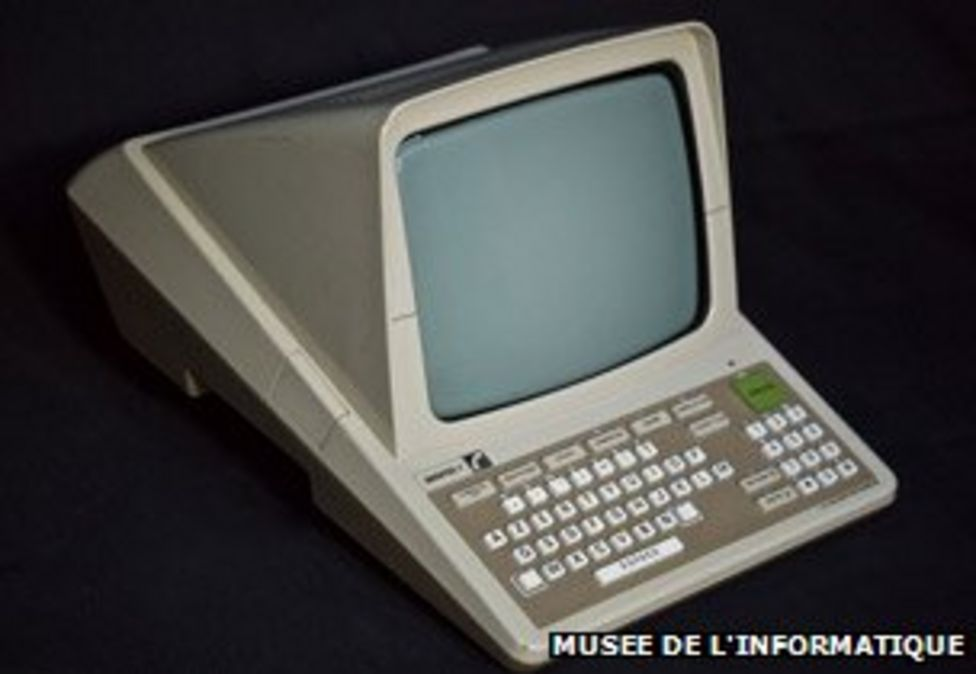
\includegraphics[width=1.0\linewidth]{../../../imagens/minitel.jpg}
                \caption{Imagem de um terminal Minitel.}
                \label{5d9a2782548e094108d5241aeff768916b33be6c}
\end{minipage}%
\hspace{0.5cm}
\end{figure}



O Judiciário brasileiro inaugurou os serviços digitais para atendimento ao cidadão, no início da década de 90. Esse pioneirismo se deu com o uso de códigos de barra para identificação de eleitores, por exemplo. Aliás, muito antes das ações do executivo, houve o desenvolvimento do sistema da Urna Eletrônica, uma iniciativa totalmente estatal, com a participação de unidades de pesquisa federais (MAMMANA et al., 1990) e (ANDRADE, 2022). As ações do executivo brasileiro em direção ao governo eletrônico remontam a década de 90, sempre com a participação do SERPRO - Serviço Federal de Processamento de Dados. Pode-se considerar que o programa de imposto de renda oferecido pela Receita Federal, a partir de, 1991 foi uma das primeiras ações em grande escala do Executivo no sentido de ofertar serviços digitais diretos para o cidadão, mesmo considerando que o envio dos dados da declaração por internet, só foi viabilizado a partir de 1998. No início, era preciso enviar os disquetes da declaração, juntamente com a documentação em papel.

O governo eletrônico ganhou mais institucionalidade no final do governo FHC, principalmente com a atuação de Pedro Parente à frente da Casa Civil (DINIZ, 2009).

O movimento do Brasil em direção ao Governo Eletrônico se deu no contexto da já mencionada tendência mundial de promover Reformas Administrativas da década de 90 e início dos anos 2000. Ramon Garcia identifica a concomitância da ação de Brasil, México e Estados Unidos, que em três anos formalizaram seus programas de Governo Digital. Brasil e México focalizaram na infraestrutura da Internet, ao passo que os Estados Unidos trabalharam para o uso da internet em serviços e processos.

O Governo Digital no Brasil foi formalizado por Decreto Presidencial, de 3 abril, de 2000  (DINIZ, 2009), cuja implementação se deu sob a coordenação política da Presidência da República, com apoio técnico e gerencial da Secretaria de Logística e Tecnologia da Informação (SLTI), do Ministério do Planejamento, Orçamento e Gestão. Essa atuação foi sustentada por um comitê, integrado pelos secretários executivos (e cargos equivalentes) dos ministérios e órgãos da Presidência da República, denominado Comitê Executivo de Governo Eletrônico (CEGE).

Inicialmente, o governo brasileiro concentrou esforços em três linhas de ação do Programa Sociedade da Informação, instituído pelo Decreto nº 3294, de 15 de dezembro, de 1999 (e depois alterado por vários instrumentos legais): universalização de serviços, governo ao alcance de todos e infraestrutura avançada.

As iniciativas do Governo FHC eram  acessíveis a uma elite de cidadãos, uma vez que a maior parte da população não tinha acesso à internet, como se vê no estudo SIDRA do IBGE (apud (SCHMITZ et al.,2021); e, embora ainda não houvesse um apontamento de soluções sistêmicas para sua universalização, essas iniciativas abriram o caminho institucional do Governo Eletrônico.

\subsection[Políticas Públicas de Inclusão e Cultura Digital]{Políticas Públicas de Inclusão e Cultura Digital}\label{Políticas Públicas de Inclusão e Cultura Digital}
As transformações, pelas quais a sociedade passava no início dos anos 90, exigiam novos paradigmas sociais, culturais e educacionais, que envolvessem estratégias de inclusão dos  cidadãos à nova realidade.

Entretanto, essa diretriz não estava presente na fase de implantação do governo eletrônico no Brasil, ainda no Governo FHC. Inicialmente, tratando os cidadãos como clientes, o foco era a redução de custos unitários, melhorias na gestão e qualidade dos serviços públicos, transparência governamental e simplificação de procedimentos - formalizados como estratégias, macro-objetivos e  as metas prioritárias  do governo brasileiro para o período de 2000 a 2003.

Paralelamente, ocorria a consolidação de uma cadeia produtiva mundial de eletroeletrônicos eficiente, que usufruía de mão de obra barata na Ásia. Esse fato contribuiu para a redução de barreiras econômicas e para o acesso a dispositivos digitais, uma vez que houve ampla comoditização da produção de eletroeletrônicos em geral e dos bens de computação em particular. Esse fenômeno era uma decorrência direta da Lei de Moore (CIPOLI, 2012), através do qual o mundo passou a produzir mais transistores eletrônicos do que grãos de soja, com ganhos de escala que tornaram essas tecnologias mais acessíveis.

Vale lembrar que a Lei de Moore foi observada empiricamente, pela primeira vez, por Gordon Earle Moore, presidente da fabricante de microprocessadores Intel, em 1965. Ele observou que a cada 18 meses a indústria de microchips eletrônicos conseguia dobrar a quantidade de transistores presentes numa pastilha de silício de área definida. Os transistores são os "tijolos" da eletrônica e são usados para processar os sinais digitais.

Essa alta disponibilidade de equipamentos digitais, a relativo baixo custo, facilitou uma presença cada vez maior da internet na vida das pessoas, principalmente a partir da popularização dos celulares do tipo "smartphone", situação que se reproduziu no Brasil no início do século XXI.

A transformação digital estimulou os governos a enfrentarem as dificuldades  de falta de  capacitação dos cidadãos na apropriação tecnológica, de forma que pudessem usufruir melhor o acesso aos equipamentos digitais. Para isso, estabeleceram políticas públicas que os preparassem para usufruírem do direito humano à comunicação, como estabelecido no Art. 19 da Declaração Universal de Direitos Humanos. Ou seja, os governos passaram a se preocupar com a inserção efetiva de seus cidadãos na Sociedade da Informação.

Essas iniciativas ficaram conhecidas como programas pertinentes a políticas de "inclusão digital" ou  de "cultura digital"; ou mesmo de "alfabetização tecnológica". Independentemente da abordagem escolhida, dentre as três indicadas, essas políticas sempre estiveram vinculadas às iniciativas de educação.

Diferentes iniciativas e perspectivas foram implementadas para uso das tecnologias da informação e comunicação no Brasil, na primeira década deste século, ao longo do segundo mandato de FHC, e do primeiro e segundo mandatos de Lula. Por meio de diferentes políticas públicas, foram disponibilizados acesso, equipamentos, aplicativos, softwares, hardwares, os quais visavam processar, armazenar, comunicar, prover apropriação tecnológica e acesso á informação e ao conhecimento.

Dentre as políticas de inclusão digital do período, destaca-se o  PROINFO - (Programa Nacional de Tecnologia Educacional) políticas de implantação de "laboratórios de microcomputadores" em escolas públicas, iniciada no Governo FHC e, substancialmente, ampliada nos Governos de Lula e Dilma.

Também, destacam-se as políticas com viés industrial, voltadas para a redução de preço dos computadores para consumidores finais; concomitantemente com a adoção de Software Livre, a exemplo do PC Conectado e o Computador para Todos.

A disseminação de Telecentros, também, teve um papel importante, criando pontos de acesso coletivo, que usufruíam do Programa GESAC, quando necessário.

Para garantir a objetividade da análise, há que se concentrar nos aspectos pertinentes ao objeto de estudo, i.e. o Programa WASH. Esta restrição exige focalizar a relação entre as tecnologias digitais e a educação, abordagem adotadas pelo programa em estudo, como se verá mais adiante.

Assim, no propósito de manter a objetividade e por sua relação direta na gênese do Programa WASH, optou-se por focalizar, neste estudo:


\begin{itemize}
\item a) política pública "Governo Eletrônico de Serviços de Atendimento ao Cidadão-GESAC", criada em 2001, programa do Ministério das Comunicações do governo FHC, cujo formato de interesse para este trabalho é o que se consolidou a partir de 2003;

\item b) Programa de Inclusão Digital da Secretaria de Inclusão Digital do Ministério de Ciência e Tecnologia, no recorte de 2005 a 2007; e
\item c) o Projeto Um Computador por Aluno (UCA), resultado da "tropicalização" da proposta americana "One Laptop per Child".
\end{itemize}

Mesmo reconhecendo que este é um capítulo de Fundamentação Teórica, parece-nos oportuno abrir parênteses para contextualizar o que vem sendo descrito até aqui, pela ótica da experiência profissional da autora. Nessa toada, cabe antecipar algo que será bastante enfatizado adiante: tivemos um papel na construção e execução de políticas públicas com as características acima, inicialmente no âmbito do Governo Eletrônico, passando pelas áreas de comunicação, saúde, cultura, e culminando na área de ciência e tecnologia.

Estes trabalhos se deram em vários momentos da carreira da autora, ao longo de quase três décadas. Isso a transformou em testemunhas ocular dos fatos, inicialmente no  município de Campinas, na década de 90, e, em seguida, no âmbito do Governo Federal, nas primeiras duas décadas do presente século.

Nessa trajetória, foi possível aprender sobre as vantagens e desvantagens de cada uma das abordagens adotadas ao longo dessas três décadas, bem como sobre a forma de combinar capacitação e estabelecimento de infraestrutura para o acesso do cidadão ao mundo digital.

A partir de uma prática regular e frequente de oficinas de formação para  crianças e adolescentes, que se iniciou em setembro de 2013, no Centro de Tecnologia da Informação CTI - Renato Archer, em Campinas, esse aprendizado se consolidou em um método, do qual essa pesquisadora é co-autora, conhecido como WASH.

Após um longo período de maturação, ajustes e repetição, esse método veio a ser formalizado em 2018, por meio de portaria de uma unidade de pesquisa do Ministério da Ciência, Tecnologia e Inovações (Portaria 178/2018 SEI/CTI).

A descrição detalhada do método consta como anexo da referida portaria, a qual sintetiza os aprendizados conquistados ao longo dos anos, pelos vários participantes do Programa. De 2018 para cá, mais aprendizados ocorreram, havendo uma necessidade de aprimoramento de sua caracterização.

É justamente uma análise sobre esse método que a presente dissertação intenciona oferecer, complementada por uma proposta de melhoria, na forma de produto educacional, como parte dos requisitos para obtenção do título de mestre, no âmbito do Mestrado Profissional em Ensino de Ciências Humanas, Sociais e da Natureza da Universidade  Tecnológica Federal do Paraná - UTFPR- Campus Londrina/PR.

\subsection[O pensamento de Papert]{O pensamento de Papert}\label{O pensamento de Papert}
Pela importância do pensamento de Papert para o Projeto One Laptop per Child (OLPC) e, portanto, para a gênese do WASH, cabe uma revisão rápida de sua obra e contribuições, permitindo uma melhor compreensão da inserção do WASH no universo conceitual das correntes pedagógicas. Essa relação entre a gênese do WASH e a proposta do OLPC ficará mais clara no capítulo de Resultados e Análise, quando a história do WASH será apresentada. Por ora, é oportuno restringirmos-nos à revisitação das contribuições de Papert.

Para conhecer  o pensamento, um pouco da história de Papert e  a filosofia do LOGO, é preciso fazer uma viagem no tempo, retornando a meados da década de 60, quando o matemático e educador sul-africano, radicado nos EUA, Seymour Papert, em colaboração com outros pesquisadores, desenvolveu a linguagem  de programação LOGO.  Foi um dos fundadores do Media Lab e diretor do grupo de Epistemologia e Aprendizado do Massachusetts Institute of Technology - MIT.

Vale ressaltar para os nativos digitais, pessoas que nasceram a partir dos anos 80 e que cresceram com essas tecnologias, que no início da era da computação, nos anos 60, os computadores existentes eram gigantes e ocupavam andares de prédios. Eram usados apenas por grandes empresas e governos e não se cogitava aplicá-los para o uso pessoal e doméstico. Poucas pessoas, com treinamento, conseguiam usar um computador. O mouse, por exemplo, nem existia ainda. Para entrar com informações nos computadores, era preciso usar cartões perfurados, inspirados nos que foram criados pelo mecânico francês Joseph-Marie Jacquard (1752-1854), que também inventou o primeiro tear automatizado, cujos padrões eram definidos nos cartões perfurados.

Papert foi um pensador visionário. Percebeu o potencial do uso da tecnologia na educação. Filósofo e pioneiro no pensar o processo de aprendizagem de crianças, de forma diferente. Em 1968, escreveu o artigo "Teaching Children Thinking", no qual abordou a temática crianças, educação e computadores:


\noindent\begin{center}\mbox{\centering\fbox{\centering\par\parbox{0.7\linewidth}{\small\textit{"Tínhamos a certeza de que, quando os computadores se tornassem tão comuns quanto o lápis, a educação mudaria tão rápida e profundamente quanto as transformações pelas quais vivíamos nos direitos civis e nas relações sociais e sexuais",(PAPERT, 1980).}\normalsize}}}\end{center}


Ele formulou esse pensamento quando os computadores dos anos 70 eram inacessíveis também para o sistema educacional. Naquele tempo, não existia o conceito de "microcomputadores" e os computadores existentes eram poucos, grandes, espalhados  (SOLOMON et al.,2020) e desajeitados, com poder de processamento e armazenagem entre milhares e milhões de vezes, inferiores ao de um notebook. Mesmo com esse baixo desempenho, os custos eram muito altos e, portanto, o acesso era muito restrito. Entretanto, valendo-se de mainframes centralizados (computadores de grande porte) com as limitações indicadas, foi possível a Papert realizar incursões no campo da aprendizagem para crianças, utilizando os computadores que estavam disponíveis, ainda que esse uso estivesse restrito a uma elite, sem a possibilidade de uma grande disseminação no sistema educacional.

Toda uma geração de educadores foi formada em torno das ideias de Papert, que defendia que a aprendizagem de linguagem de programação de computadores, já no ensino fundamental, poderia ter um papel importante no aprendizado de muitas outras disciplinas tradicionais, principalmente a matemática, mas também gramática (SOLOMON et al.,2020), entre outras.

Entendemos que a proposta de Papert, até por enfatizar o aprendizado de crianças, não tinha qualquer ambição de capacitação profissional e, por si, não visava diretamente fazer frente aos desafios do "mundo do trabalho", que foram sendo introduzidos pelas transformações inerentes à Sociedade da Informação, nas décadas subsequentes.

Em sua obra "A Máquina das Crianças" (1994), Papert discorre sobre a importância da tecnologia e sua inserção na educação, a fim de melhorar a qualidade do ambiente de aprendizagem.


\noindent\begin{center}\mbox{\centering\fbox{\centering\par\parbox{0.7\linewidth}{\small\textit{"Nós podemos dar um poder sem precedentes para as crianças inventarem e desenvolverem projetos excitantes, provendo o acesso a computadores, com uma linguagem de programação adequada, inteligível e clara, bem como com periféricos capazes de produzir uma ação on-line/real-time" (SOLOMON et al., 2020).}\normalsize}}}\end{center}


Segundo o autor, "ao redor do mundo inteiro, as crianças entraram em um apaixonante e duradouro caso de amor com os computadores" (1994, p.07).

Essa filosofia e a maneira de colocar em prática a criança epistemóloga vieram do seu aprendizado na relação de trabalho e convivência com Piaget.

Papert ficou impressionado de ver as crianças, construtoras de suas próprias estruturas intelectuais [Logo, computadores e educação, pág 35]:


\noindent\begin{center}\mbox{\centering\fbox{\centering\par\parbox{0.7\linewidth}{\small\textit{A linguagem LOGO faz com que o computador deixe de ser apenas um meio de transferir informação e passe a ser a ferramenta, com a qual a criança pode formalizar os seus conhecimentos intuitivos. (PAPERT, 1980)}\normalsize}}}\end{center}


Essa nova relação com a computação, proposta por Papert, permitiu uma transformação na educação e no processo de ensino e aprendizagem, colocando o computador como relevante para o ensino fundamental, mas sempre entendendo a criança como programadora e não apenas como usuária.

Papert examinou as crianças que tinham aprendido a programar computadores e identificou que elas podiam usar os modelos concretos para "pensar sobre o pensar" e "aprender sobre o aprender"  (PAPERT, 2005), estimulando-as  a aumentarem seus poderes de epistemólogos. Sobre isso, ele discorreu no artigo publicado, em 1970, intitulado Teaching Children Thinking.

Segundo José Armando Valente, um dos responsáveis, em conjunto com a Professora Afira Vianna Ripper, pela tradução do livro LOGO: computadores e educação: "Papert acreditava que o computador era a ferramenta que propiciava às crianças as condições de entrar em contato com algumas das mais profundas ideias em ciência, matemática e a criação de modelos".

Programar, na filosofia LOGO, significa "comunicar-se com o computador, numa linguagem que tanto ele, quanto o homem,  podem entender". Toda criança aprende a falar. Por que, então, não deveria aprender a "falar" com um computador?", indagava Papert  (PAPERT, 1980).

A proposta de Papert envolvia, também, a ideia de que o computador pudesse ser um interlocutor  de matemática ou um interlocutor de línguas. Nessa concepção, o LOGO, ao ser um interlocutor da matemática, contribui, de uma maneira lúdica, para superar as barreiras matofóbicas (fobia por matemática e fobia pelo aprendizado), transformando a matemática, que passa a ser uma língua viva (PAPERT, 1980) .

Papert abordou sobre a "matofobia: o medo de aprender", com duas associações: o conhecido medo da matemática, que tem a intensidade de uma verdadeira fobia; e o  significado do radical mathe, que, em grego, significa aprender.


\noindent\begin{center}\mbox{\centering\fbox{\centering\par\parbox{0.7\linewidth}{\small\textit{"A matofobia pode cultural e materialmente limitar a vida das pessoas. Muitas outras pessoas ainda não desistiram completamente de aprender, mas sentem-se impedidas por opiniões negativas, arraigadas sobre suas capacidades. A deficiência torna-se uma identidade, "não consigo aprender francês, não tenho ouvido para línguas, nunca poderia ser um homem de negócios, não tenho cabeça para contas. Essas crenças são superstições e estão presentes em nosso cotidiano, elas criam tabus para a aprendizagem. Se as pessoas acreditam que não podem entender matemática, conseguiram abster-se de tentar executar qualquer coisa que reconheçam a matemática, gerando como consequência uma auto-sabotagem"  (LOGO: Computadores e educação, PAPERT, S. pg.62, 63)}\normalsize}}}\end{center}


Papert chamou atenção quanto à separação, imposta por nossa cultura, entre o verbal e o matemático. Tornou-se muito comum falar como se houvesse diferentes cérebros ou mesmo órgãos separados no cérebro, para matemática e linguagem.

Em suas vivências com as crianças, Papert materializava o pensamento abstrato da matemática. Ao construírem os seus jogos, primeiro, as crianças faziam o movimento com o seu corpo, para, depois, usar os comandos do LOGO. A ilustração deste processo pode ser vista no vídeo  da entrevista, realizada com a Professora Afira Ripper,  um dos produtos desta dissertação (ver no capítulo de Produtos Educacionais).

As crianças são permeadas por ideias de que há pessoas boas em matemática e outras que não podem entender matemática; mas, Papert acreditava que a presença do computador poderia neutralizar a matofobia (PAPERT, 1980) .

Papert criticou o modo como os computadores estavam sendo usados na educação americana, ou seja, estavam sendo usados para fornecer informações ou instrumentos de instrução assistida por computador (CAI-Computed Aid instruction)  (PAPERT, 2005).

Segunda a percepção do autor, o tipo de abordagem existente materializava a ideia do computador programando a criança (PAPERT, 2005). O LOGO, enquanto linguagem de programação pensada para as crianças, tinha como proposta inverter essa relação.

Papert pôde conferir, com as crianças em idade pré-escolar, que é possível ela controlar a máquina e ser protagonista na programação do seu computador. Com isso, ao ensinar o computador a pensar, ela explora a sua própria forma de pensar.

Teaching Children Thinking, artigo escrito por Papert, foi a primeira publicação que sugeria que a criança poderia ficar no comando da máquina e não a máquina no comando da criança.  Esse artigo  foi publicado em 1970; e,  apresentou um novo processo para a educação, em que os computadores pudessem serem usados para a criatividade.

Papert apresentou uma nova ideia: de que "ensinar o pensamento"  é apropriado para a escola primária, mas essa não era a corrente principal da educação americana, naquele contexto.

O LOGO, segundo Papert, proporcionou a milhares de professores do ensino básico a sua primeira oportunidade para apropriar-se do computador, de maneira que ampliaram seus estilos pessoais de ensinar. ( Papert, S, "A maquina das crianças, repensando a escola da era da informática", pg.57).

Em seu percurso de pesquisa, na apresentação do LOGO, na experimentação, seja com as crianças ou com os professores, Papert encontrou o que ele chamava de "professores conservadores e  inovadores" (PAPERT, 1980).

Outro aspecto importante na obra e vivência de Papert é quanto aos modos hierárquicos de pensar sobre o conhecimento. Ele adotou o termo  " heterarquia " para descrever a forma de aprendizagem pretendida, um conceito presente em  "A máquina das Crianças". Trata-se de  um termo oposto à hierarquia, comum na forma de trabalho da escola tradicional. Como vimos na seção 2.1.2, na heterarquia, cada elemento é igualmente governado por todos os outros.

Mais adiante será possível mostrar que o WASH se estruturou numa forma de heterarquia, assunto que será tratado nos resultados.

A proposta de Papert para o Governo Federal, em 2005, não foi a primeira oportunidade de interação com o poder público brasileiro.

Em 1989, quando a prefeita eleita Luiza Erundina de Souza assumiu a Prefeitura de São Paulo, convidou o Prof. Paulo Freire para assumir a pasta de educação. Um novo projeto político-educacional foi elaborado a partir de uma reavaliação dos existentes. A partir dessa iniciativa, foi recriado o projeto de Educação e Informática da Secretaria Municipal de Educação de São Paulo, fundamentando-se na tese de que:


\noindent\begin{center}\mbox{\centering\fbox{\centering\par\parbox{0.7\linewidth}{\small\textit{[…] uma sociedade informatizada está passando a exigir homens com potencial de assimilar a "novidade" e criar o novo, o homem aberto para o mundo, no sentido que lhe confere a teoria piagetiana quando se refere às assimilações mentais majorantes; da mesma forma, exige a presença do cidadão crítico e comunitário, onde os artefatos tecnológicos, especificamente o computador, possam ser ferramentas auxiliares para a construção de uma sociedade mais igualitária e justa. (SÃO PAULO, 1992 , p. 7). Em 1995, Paulo Freire.}\normalsize}}}\end{center}


Ao longo da consolidação dos conceitos descritos até aqui, Papert estabeleceu uma vertente do construcionismo com grandes resultados práticos, tendo inaugurado a base para uma cultura de aprendizagem baseada no "fazer", sustentada em ideias como:


\begin{itemize}
\item A criança deve estar no centro do processo de aprendizagem, conduzindo-na sempre que possível;
\item Não existe idade ideal para aprender as coisas: cada criança tem o seu próprio tempo e momento de interesse; e
\item Das próprias palavras de Papert: "a meta é ensinar de forma a produzir a maior aprendizagem, a partir do mínimo de ensino"  ([[PAPERT, 1994]]).
\end{itemize}

Com estes conceitos, Papert indica a necessidade de estimular as crianças a fazerem suas próprias pescarias,  (PAPERT, 1994) com vistas a obter o conhecimento.

Complementam essas ideias,os conceitos de (PAPERT, 1999):


\begin{itemize}
\item Learn by doing ou aprender fazendo: a ideia, em parte,  do senso comum em parte originada, por Dewey, é aprender ao longo do processo de fazer coisas que realmente nos causa interesse;
\item Technology as a building material, ou "tecnologia como um material de construção": a tecnologia nos permite fazer muito mais, à medida que aprendemos, porque ela nos empodera, com seus recursos, para alcançar características em nossas produções, seja um jogo, protótipo ou peça de comunicação, por exemplo, que não conseguiríamos sem ela;
\item Hard fun ou "diversão desafiadora": existe um entendimento de que aprende-se melhor quando nos divertimos, mas a diversão não requer que a atividade seja fácil. É preciso garantir que a aprendizagem, mesmo sendo divertida, tenha um caráter de desafio, que instigue o educando.
\item Learn to learn ou "aprenda a aprender": o conceito subjacente é o de protagonismo do educando na aprendizagem, implicando que a ideia de ensinar é muito menos importante do que a ideia de aprender.
\item Taking time ou "assumindo o controle do seu próprio tempo": os estudantes devem, ao assumir o protagonismo de sua aprendizagem, gerenciar o próprio tempo e suas próprias atividades, sem a necessidade de alguém lhes dizendo o que fazer;
\item You can’t get it right without getting it wrong ou "você não consegue acertar
se não errar primeiro"é o conceito de que para aprender é preciso existir a
liberdade para errar. As coisas importantes nunca funcionam da primeira vez, e ao tentar corrigí-las é que o processo de aprendizagem ocorre;
\item Do unto ourselves what we do unto our students ou "façamos conosco o que fazemos com nossos estudantes": este conceito é direcionado aos educadores, que precisam adotar para si a ideia de que, também, vão aprender fazendo e também vão aprender errando. A melhor lição para nossos estudantes é deixá-los nos assistir, "sofrendo" durante o nosso próprio aprendizado;
\item We are entering a digital world ou "nós estamos entrando em um mundo digital": conhecer e saber atuar dentro do mundo digital é tão importante quando ler ou escrever.
\end{itemize}

Mitchel Resnick, do Grupo Lifelong Kindergarten, MIT, baseado nas ideias construcionistas de Seymour Papert, apresenta, em 2007, o Scratch, como uma ferramenta para a aprendizagem criativa, considerando os 4 Ps da aprendizagem criativa: projetos, paixão, pares e pensar brincando (play). A iniciativa de Resnick se consolidou. É por isso que, hoje, você pode encontrar no Scratch um aliado no processo de aprendizagem. O Scratch reúne uma comunidade ativa, da qual fazem parte quase 50 milhões de crianças, jovens e adultos do mundo inteiro. O coordenador do Programa WASH teve a oportunidade de conhecer uma das primeiras versões do Scratch, descrita pessoalmente pelo Prof. Resnick, 2007.

O Programa WASH, seguindo nossa hipótese de que tem gênese nas propostas do OLPC, se inspirou na metodologia subjacente ao Scratch e, desde os primórdios, tem como base o uso desse instrumento nas atividades de educação. O WASH estimula a cultura digital no turno e contraturno escolares e oferece oficinas, que não podem ser classificadas como aulas tradicionais, porque abdicam de roteiros, apostilas e conteúdos fixos, uma característica muito presente nos métodos criados pelos pensadores do MIT, discípulos de Papert. Nessa concepção, o educando aprende, fazendo e errando, com objetivos determinados e oportunidade para tentar de novo. Assim, embora haja uma abertura muito grande para a experimentação de propostas variadas, o Programa WASH oferece, como linha básica de ação, a programação de jogos, usando a linguagem Scratch, e isto será visto adiante.

Ao usar o Scratch, nas oficinas do Programa WASH, estamos oportunizando e estimulando "as crianças e jovens a serem criativas, produzirem seus jogos, suas narrativas, suas animações, o raciocínio lógico, contribuindo com o letramento digital, colaborando com a alfabetização científica, e para não serem somente consumidores de jogos, games, mas produtores, também".

Os resultados do emprego do Scratch, no Programa WASH serão discutidos em Resultados e Análise; mas pode-se antecipar que envolveram milhares de crianças e jovens, produzindo jogos, com os bolsistas de iniciação científica aprendendo com o ensinar, multiplicando e compartilhando o conhecimento das ferramentas digitais  com a comunidade, tanto por meio das oficinas do WASH, quanto pela participação em feiras, eventos e congressos.

Em nossa vivência, a tartaruga, de Seymour Papert; e o gato, de Mitchel Resnick,  representam as bases da  programação e com eles aprendemos a  programar, brincando.

\subsection[O LOGO e o SCRATCH]{O LOGO e o SCRATCH}\label{O LOGO e o SCRATCH}
O LOGO é uma linguagem de programação, desenvolvida em 1966 por Seymour Papert, Wallace Feurzeig, Daniel Bobrow e Cynthia Solomon (ver Fig. 4), no âmbito dos laboratórios Bolt, Beranek and Newman, Inc (BBN) and MIT Artificial Intelligence Lab (SOLOMON et al., 2020). O LOGO foi muito difundido no contexto educacional a partir daquela década, tendo ajudado gerações de crianças a aprender várias disciplinas, mas principalmente matemática (SOLOMON et al.,2020).



\captionsetup{format=plain}
\begin{figure}[p]

\centering


\begin{minipage}[b]{0.4\linewidth}
        \centering
                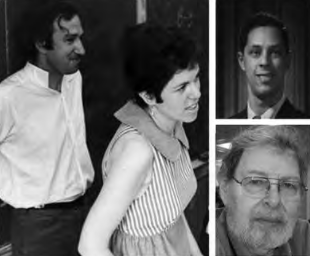
\includegraphics[width=1.0\linewidth]{../../../imagens/criadores-logo.png}
                \caption{Criadores do Logo em 1966: Seymour Papert, Cynthia Solomon, Danny Bobrow e Wally Feurzeig (fonte: (SOLOMON et al,2020)}
                \label{c40acbbf355efda753f44d02f297bbce67f5e4b8}
\end{minipage}%
\hspace{0.5cm}
\begin{minipage}[b]{0.4\linewidth}
        \centering
                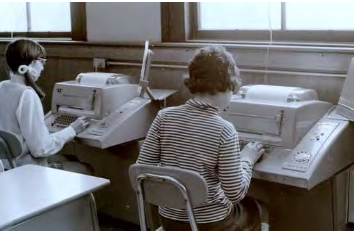
\includegraphics[width=1.0\linewidth]{../../../imagens/criancas-1968.png}
                \caption{Crianças de 12 anos da Muzzey Junior High School usando LOGO em terminais teletipo (Fonte: (SOLOMON et al. (2020, 1968).}
                \label{1a5368da06f895c87008b3fc1675ccfbb494f1f9}
\end{minipage}
\hspace{0.5cm}
\begin{minipage}[b]{0.4\linewidth}
        \centering
                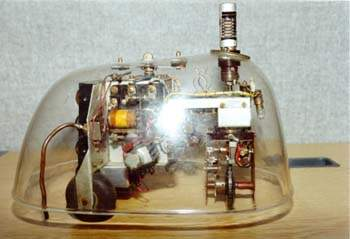
\includegraphics[width=1.0\linewidth]{../../../imagens/Elmer-Elsie4.jpg}
                \caption{Elmer e Elsie eram dois robôs com rodas, chamados de cágados (tortoise), que podiam se deslocar pelo chão. Foram desenvolvidos pelo Inglês Grey Walter.}
                \label{fdc1f0b8e99c3e3a345c88c79ff4e953d65b3424}
\end{minipage}%
\hspace{0.5cm}
\begin{minipage}[b]{0.4\linewidth}
        \centering
                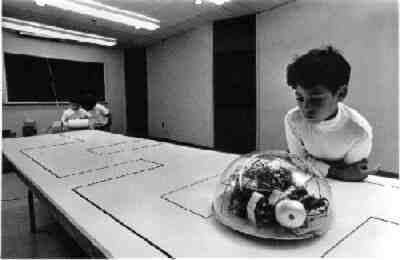
\includegraphics[width=1.0\linewidth]{../../../imagens/historia-logo-turtle-01.jpg}
                \caption{Em foto de 1969, uma criança observa o primeiro robô tartaruga criado no MIT (Fonte: (CIBERNECTZOO (2010).}
                \label{c2ca828982a83621e08977a23628db7b32a934d9}
\end{minipage}
\hspace{0.5cm}
\begin{minipage}[b]{0.4\linewidth}
        \centering
                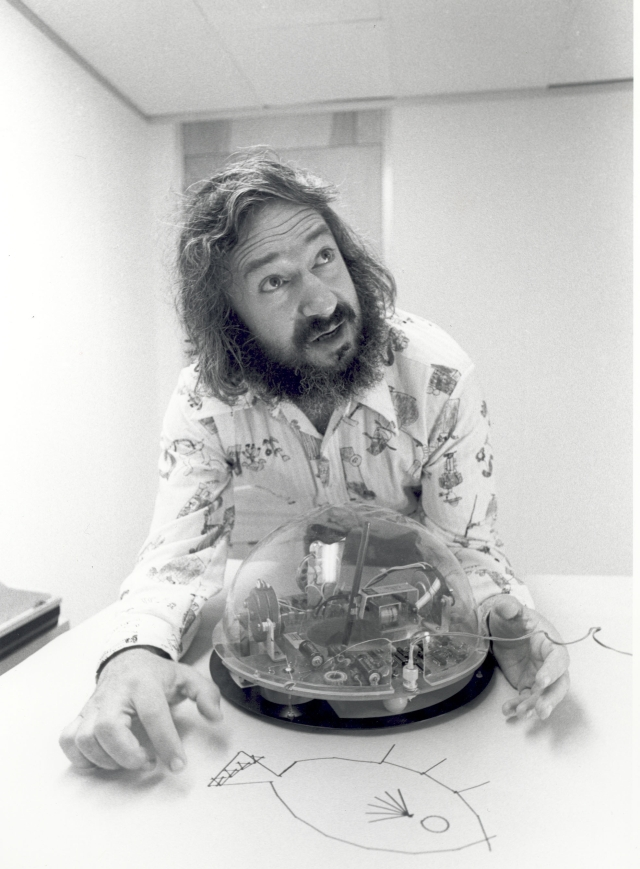
\includegraphics[width=1.0\linewidth]{../../../imagens/Papert-x640.jpg}
                \caption{Papert com uma de suas tartarugas robôs. (Fonte:  [[CIBERNECTZOO (2010)]])}
                \label{16372e5cf76e6860245131e51a3bf17c58dd1e46}
\end{minipage}%
\hspace{0.5cm}
\begin{minipage}[b]{0.4\linewidth}
        \centering
                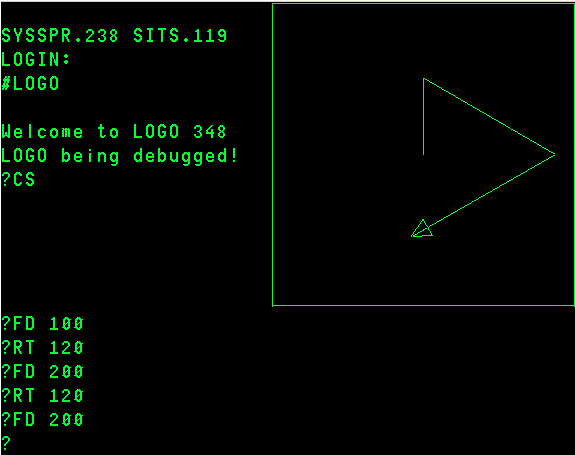
\includegraphics[width=1.0\linewidth]{../../../imagens/logo-PDP11.png}
                \caption{Imagem de uma tela do LOGO num terminal gráfico da década de 70, provavelmente rodando em um PDP11. O triângulo pequeno é a tartaruga (Fonte: gunkies.org).}
                \label{ca83b217b58f57e503ff496c6c6f47bee5dc77cd}
\end{minipage}
\hspace{0.5cm}
\end{figure}



No LOGO, a construção se dá pela criação, junção e reaproveitamento de algoritmos de computador, como num jogo de encaixe.

O LOGO possibilita a definição de novos comandos e funções, numa configuração interativa, que permite visualizar e vivenciar os resultados, à medida que os programas são construídos. Considerando que o LOGO foi criado na década de 60, já se tratava de uma inovação num período em que a interface de muitos computadores ainda era baseada em cartão perfurado.

Desta forma, pode-se dizer que o LOGO nunca foi um mero brinquedo; mas, ao contrário, se constitui em uma poderosa linguagem de computação, planejada para fornecer acesso à programação para principiantes, visando estimular a aprendizagem.

O LOGO é associado à imagem de seu cursor, uma tartaruga que percorre a tela deixando um rastro que forma as figuras geométricas desejadas. Entretanto, poucas pessoas sabem que em seu início, a linguagem "focava em brincar com palavras e sentenças" ([[SOLOMON et al., 2020]]), sendo que sua tartaruga " icônica " apareceu depois.  [[SOLOMON et al. (2020)]] menciona que o aprendizado sem a tartaruga podia ocorrer no campo da gramática, por exemplo, quando as crianças, independentemente de recursos visuais, demonstravam uma apreciação por sistemas formais.

A Fig. 5 mostra a experiência de utilização do LOGO com alunos do sétimo ano na Escola Muzzey Junior High School, na cidade de Lexington, em Massachussetts. Naquela experiência, os estudantes desenvolveram o jogo Pig Latin, Vinte Questões, Nim, SENGEN (gerador de sentenças), ensino de matemática e contador de histórias  ([[SOLOMON et al., 2020]]). Eram usados terminais teletipos sem tela e ainda não existia o conceito de tartaruga.

A ideia do ícone da tartaruga surgiu quando a experiência da Escola Muzzey estava chegando ao fim, em 1969. As crianças tiveram uma boa experiência com a diversidade de projetos de programação, que focavam em palavras, e sentenças, ainda sem as tartarugas; mas Papert queria expandir os domínios de exploração pelas crianças ([[SOLOMON et al., 2020]]). Para isso, foi pensado que era necessário criar um objeto concreto para se brincar, algo que pudesse ser controlado diretamente pelas crianças. Papert se inspirou nos "cágados"  (tortoise) robôs de William Grey Walter. "Elmer and Elsie" (ver Fig. 6) tinham rodas, motores e sensores e podiam se deslocar pelo chão da sala ou sobre uma mesa, sendo conectados ao computador por um cabo (tether) num primeiro momento. Logo em seguida foram substituídos pela imagem de tartarugas numa tela de computador, ([[SOLOMON et al., 2020]]). A Fig. 7 mostra uma criança de 1969 observando o primeiro robô tartaruga criado no MIT, a Fig. 8 mostra Papert com uma de suas tartarugas e a Fig. 9 mostra a imagem de uma tela de um computador PDP11 rodando LOGO na década de 70.

Com o avanço da tecnologia e a disponibilização de interfaces humano-computador, cada vez mais avançadas (displays melhores, mouse, tablets, etc.), o longevo LOGO começou a sentir o peso da idade.

Em [[SOLOMON et al. (2020)]] é mencionado o valor de uma alternativa ao LOGO, que pudesse tirar proveito das virtudes das chamadas "linguagens de programação visual", uma vez que reconheciam:


\noindent\begin{center}\mbox{\centering\fbox{\centering\par\parbox{0.7\linewidth}{\small\textit{"Os jovens iniciantes em LOGO dedicavam muito tempo caçando letras no teclado" ([[SOLOMON et al., 2020]])}\normalsize}}}\end{center}


A alternativa veio na forma de linguagem Scratch, criada por Mitchel Resnick e seus estudantes. Mitchel, em 1989, já tinha se dedicado ao desenvolvimento de uma versão do LOGO, com múltiplas tartarugas (StarLogo). As discussões sobre a necessidade de um  LOGO visual começaram logo depois, em 1990, mesmo com a visão de Papert que uso de uma interface visual significaria apenas uma mudança de representação, o que não faria muita diferença   ([[SOLOMON et al., 2020]]). Mitchel Resnick, segundo  [[SOLOMON et al. (2020)]], "não compartilhava desse pessimismo" e pressionou para que uma linguagem em blocos simples fosse criada e testada. Sobre o teste,  [[SOLOMON et al. (2020)]] se manifesta como segue:


\noindent\begin{center}\mbox{\centering\fbox{\centering\par\parbox{0.7\linewidth}{\small\textit{"Para a minha surpresa, mas não para a surpresa de Mitchel, o teste funcionou realmente bem. O que Seymour e eu não tínhamos antecipado é que o fato da linguagem parecer simples aumentava a vontade das pessoas se engajarem nos estágios iniciais da experiência de programação, comparativamente com a forma não visual. Em certo sentido não era mais simples, mas o que importa é que parecia mais simples.  ([[SOLOMON et al., 2020]], tradução livre)}\normalsize}}}\end{center}


Assim, depois de uma série de desdobramentos e desenvolvimentos, Mitchel Resnick apresenta, em 2007, o Scratch, como uma ferramenta para a aprendizagem criativa. A iniciativa de Resnick se consolidou, criando as condições para que fosse disponibilizada uma ferramenta poderosa de programação, encapsulada num formato lúdico e atraente para crianças, que funciona como um aliado no processo de aprendizagem. A Fig. 10 mostra um trecho de código em Scratch, organizado na forma de blocos.



\captionsetup{format=plain}
\begin{figure}[p]

\centering


\begin{minipage}[b]{0.4\linewidth}
        \centering
                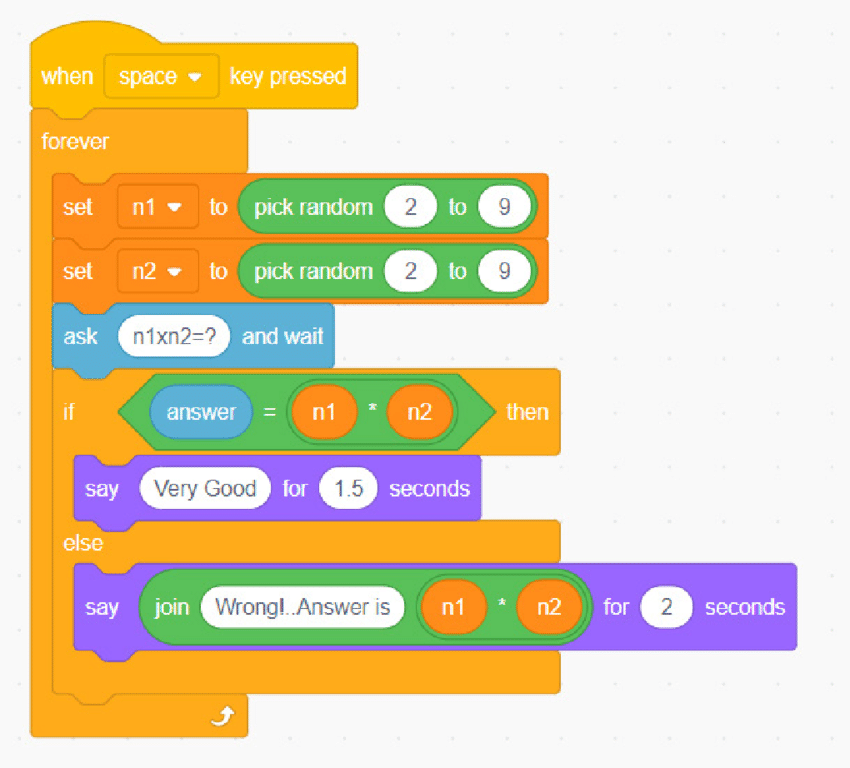
\includegraphics[width=1.0\linewidth]{../../../imagens/Scratch-Block.png}
                \caption{Trecho de um código em Scratch, em que se vê a organização por blocos, que podem ser montados como num jogo de encaixe. (Fonte: u [[SUNG (2019)]])}
                \label{5cac9c9edeb34a88b5571069bb494cda1ce1bd9c}
\end{minipage}%
\hspace{0.5cm}
\end{figure}



O Scratch reúne uma comunidade ativa, da qual fazem parte quase 50 milhões de crianças, jovens e adultos do mundo inteiro. O Coordenador do Programa WASH teve a oportunidade de conhecer uma das primeiras versões do Scratch, descrita pessoalmente pelo Prof. Resnick, na época de seu desenvolvimento.

Ainda há questionamentos sobre a acessibilidade do Scratch, por seu caráter visual, cabendo aos pesquisadores do mundo todo se debrucem sobre a questão do design universal, para que pessoas cegas, principalmente, possam usufruir dos mesmos benefícios da ferramenta, que hoje está restrita aos videntes.

\subsection[O que é STEM/STEAM?]{O que é STEM/STEAM?}\label{O que é STEM/STEAM?}
Vários autores ([[CATTERALL, 2017]])  ([[GONZALES e KUENZI, 2012]])  ([[JANKOSKI, 2017]])  ([[BYBEE, 2010]]) indicam a década de 90 do século passado como o início do uso estruturado do conceito de Science, Technology, Engineering and Mathematics (STEM) em currículos escolares, mas o acrônimo para representá-lo teve alterações ao longo dos anos. 
Segundo post de  [[JANKOSKI (2017)]], inicialmente o conceito era representado pela sigla SMET, mas a similaridade de pronúncia com a palavra "smut (que significa obscenidade, em inglês) sugeriu a mudança da sigla para METS e depois para STEM, em 2001  ([[BRITANNICA, 2022a]]).

Autores mencionam a confusão que este termo gera, uma vez que em inglês pode se referir a células tronco, com tronco de árvore ou com o pedestal de um copo de vinho  ([[BYBEE, 2010]]). Para evitar esse tipo de confusão, é possível identificar uma recorrência da forma "STEM Education" nas publicações. Neste trabalho, será usada a forma STEM, em maiúsculas, para se fazer referência ao movimento de revisão curricular associado às disciplinas de "Science, Technology, Engineering and Mathematics.

Os Estados Unidos sempre deram importância para a educação de ciências como política pública. Uma evidência disso pode ser encontrada nas atas da Convenção Constitucional de 1787, a exemplo do que se extrai da "Notes of Debates in the Federal Convention of 1787  ([[GONZALES e KUENZI, 2012]]):


\noindent\begin{center}\mbox{\centering\fbox{\centering\par\parbox{0.7\linewidth}{\small\textit{"to establish seminaries for the promotion of literature and the arts and the sciences.}\normalsize}}}\end{center}


Outra evidência pode ser extraída do primeiro discurso do Presidente George Washington do Estados Unidos da América:


\noindent\begin{center}\mbox{\centering\fbox{\centering\par\parbox{0.7\linewidth}{\small\textit{"Nor am I less persuaded that you will agree with me in opinion that there is nothing which can better deserve your patronage than the promotion of science and literature. Knowledge is in every country the surest basis of public happiness. In one in which the measures of government receive their impressions so immediately from the sense of the community as in ours it is proportionably [sic] essential. 2 (First State of Union Address - President George Washington)}\normalsize}}}\end{center}


Da mesma forma, autores como  [[BYBEE (2013)]]  ou  [[GONZALES e KUENZI (2012)]] traçam o lançamento do satélite Sputnik, em 1950, como um divisor de águas para o ensino de STEM, nos Estados Unidos.

O movimento pelo STEM, naquele país, tem evidente motivação econômica, estratégica e de manutenção da hegemonia americana. Uma evidência disso é a citação à fala do Presidente da Lockheed Martin, Norm Augustine, em outubro de 2012, presente em  [[CATTERALL (2017)]]:


\noindent\begin{center}\mbox{\centering\fbox{\centering\par\parbox{0.7\linewidth}{\small\textit{"... industry and government to promote more STEM education in the U.S. ‘Failure to do so... will undermine the U.S. economy, security and place as a world leader.’ Competing with knowledge-based resources will be one way that the U.S. can recover and retain primacy in the global marketplace (Twittweb, 2012).}\normalsize}}}\end{center}


Mas, em termos recentes, foi em meados da década de 90 que o baixo desempenho comparativo em STEM dos estudantes americanos ganhou notoriedade na imprensa, pela constatação de uma sequência de notas medíocres no Programme for International Student Assessment (PISA)  ([[CATTERALL, 2017]]). O PISA é um exame internacional promovido pela Organização para a Cooperação e Desenvolvimento Econômico (OCDE), que busca estabelecer um padrão global de avaliação, que permita comparar o desempenho de estudantes de diferentes países. Nos dias de hoje, estudantes de cerca de 65 países participam do exame, que é considerado um instrumento importante para planejar melhorias nos sistemas educacionais ao redor do mundo.

Em 1998, por meio de um relatório apresentado ao Congresso Americano pelo Committee on Equal Opportunities in Science and Engineering da National Science Foundation, este organismo, que seria o equivalente ao nosso CNPq, alerta para a importância do ensino de STEM nas escolas fundamentais americanas, para que os EUA mantenham sua liderança global  ([[CONGRESS, 1998]]):


\noindent\begin{center}\mbox{\centering\fbox{\centering\par\parbox{0.7\linewidth}{\small\textit{"In order to maintain its global leadership, America must ensure our citizens can meet the demands of a more scientifically- and technologically-centered world. The National Science Foundation (NSF) has a key role in creating and maintaining the science, mathematics, engineering, and technology (SMET) capacity in this nation. The Committee on Equal Opportunities in Science and Engineering (CEOSE) has been charged by Congress with advising NSF in assuring that all individuals are empowered and enabled to participate fully in the science, mathematics, engineering, and technology (SMET) enterprise.}\normalsize}}}\end{center}


No relatório, o NSF usa ainda o acrônimo SMET que, em 2001, segundo a enciclopédia Britânica teria sido alterado para STEM ([[BRITANNICA, 2022a]]).

As áreas em que os estudantes americanos não conseguiam se sobressair, em relação aos demais países desenvolvidos, eram as de ciências, tecnologia e matemática  ([[CATTERALL, 2017]]). Essa situação passou a representar incômodo para os gestores educacionais do país, dado que não refletia a sua imagem própria de potência internacional  ([[CATTERALL, 2017]]), principalmente no campo da ciência e tecnologia. Foi nesse momento que as iniciativas educacionais em "science, technology, engineering and mathematics se destacaram e o acrônimo SMET surgiu, posteriormente substituído por STEM  ([[CATTERALL, 2017]]).

Segundo a interpretação da época, o baixo desempenho americano em STEM tinha relação com a falta de equidade no acesso ao STEM, dentro da realidade das escolas americanas  ([[CATTERALL, 2017]]).

Dentre as respostas do governo americano, destacaram-se o programa "Nenhuma Criança Deixada para Trás", em tradução livre de "No Child Left Behind Act", uma iniciativa de 2002, e o "Todo Estudante terá Sucesso", em tradução livre de "Every Student Succeeds, de 2015  ([[CATTERALL, 2017]]).

Mas, as respostas americanas não ficaram restritas às esferas de governo, havendo também as que foram conduzidas por organizações não-governamentais, universidades, think-tanks, entre outras.

Em termos epistemológicos, podemos dizer que o STEM é o sincretismo de diferentes visões do método científico, cabendo uma análise individual de cada um, identificado pela primeira letra do acrônimo STEAM.

De acordo do relatório do WASH enviado ao [[CNPq (2020)]], fizemos uma discussão sobre a epistemologia subjacente a cada um dos elementos. Sentimo-nos confortáveis com a reprodução das ideias aqui, recompiladas, uma vez que somos coautores do referido relatório. Como exemplos do que descrevemos concentramos-nos na indústria de semicondutores, área de domínio do co-orientador desta dissertação, bem como no campo dos instrumentos de percussão, área na qual esta autora investiu tempo, através de sua participação no grupo cultural "Caixeirosas". A escolha dos semicondutores (ou chips) como exemplo é oportuna, também, porque são esses dispositivos, os viabilizadores das tecnologias digitais, fundamentais para a existência, nos dias de hoje, de uma "cultura digital". Os chips são imprescindíveis para todos os dispositivos digitais, não havendo tecnologia substituta.

Um dos pontos altos da discussão a seguir é trazer a interdependência dos 5 elementos do STEAM.

É razoável considerar o método de engenharia (E) como sendo derivado do método científico (S), havendo uma grande interdependência entre os resultados de um no outro; muito embora seus objetivos sejam diferentes. O desenvolvimento tecnológico (T) tem na engenharia (E) sua aliada e pode ser considerado, em alguma situações, como decorrente dela, principalmente quando se faz referência ao termo "alta tecnologia". Mas não basta um produto ser baseado em algum conhecimento científico para que seja alta tecnologia. De forma genérica, é possível dizer que "alta tecnologia " é uma alusão a processos de manufatura complexos, com muitas etapas de alto grau de risco de sucesso cada uma, o qual pode ser mitigado através do emprego de alguma forma de conhecimento científico.

Um exemplo de alta tecnologia é a manufatura de circuitos integrados ou chips. Os chips são circuitos eletrônicos ultra-miniaturizados cuja produção requer entre dezenas e centenas de etapas de processo. A existência de uma "Cultura Digital" é diretamente relacionada ao sucesso da indústria de chips, que, além de desenvolver os dispositivos em si, que sustentam as redes digitais contemporâneas, conseguiu desenvolver os conhecimentos necessários para contornar o alto risco de suas etapas de produção, conduzindo para um processo que hoje tem alta produtividade. Nesse exemplo dos chips, a engenharia teve papel preponderante e muitos outros exemplos da contribuição da engenharia para a tecnologia podem ser citados.

Por sua relação com a engenharia, é natural considerar que a tecnologia também pode estar relacionada ao método científico, muito embora não devesse ser confundida com a ciência em si. As pessoas tendem a confundir os conceitos de tecnologia e ciência, assumindo que a primeira (T) é decorrente da segunda (C). Entretanto, defendemos que não existe dependência intrínseca entre tecnologia e ciência. Os processos que levam ao estabelecimento de (T) podem ter contextos cognitivos, sensoriais e culturais não formais, independentes de (C). Então, vale a pena refletir sobre situações em que a tecnologia pode se desenvolver por outros meios, que não os científicos.

Aproveitando os resultados de nossa reflexão registrada em  [[CNPq (2020)]], vamos nos debruçar de forma um pouco mais estendida sobre essa questão, criando uma hipótese sobre o desenvolvimento de instrumentos musicais.

O ser humano tem a necessidade constante de expressar seus sentimentos e emoções, e faz isso através do estímulo às percepções e sensações em si e nos outros. Reduzida a um contexto instrumental, a arte (A) pode ser considerada como uma concretização da comunicação dessas percepções e sensações entre os indivíduos, tendo um caráter muito mais amplo do que a própria ciência, a tecnologia ou a engenharia. Por outro lado, o estímulo mútuo sempre requer alguma forma de interação por meio, dos sentidos, a qual, por sua vez, exige o emprego de meios materiais, diretos ou indiretos. Por exemplo, a arte pode depender de instrumentos musicais, de tintas coloridas ou de ferramentas de corte para esculpir, por exemplo. Todos estes meios têm um certo grau de dependência dos conhecimentos da ciência, da engenharia e da tecnologia.

Em oposição, podemos imaginar situações em que as artes plásticas são desempenhadas por artesãos ou outros profissionais artistas sem reconhecimento acadêmico formal, mas que dominam gestos e técnicas complexos. Quando o homem esticou a primeira pele de animal para produzir um tambor primitivo, talvez (apenas por hipótese) tenha sido motivado pela necessidade orgânica de reproduzir sons periódicos, tais como seus próprios batimentos cardíacos. Eles sutilmente acompanham os seres humanos por toda a vida e têm um papel na noção de ritmo. É impossível ter certeza, mas podemos imaginar, como apoio retórico, de que forma o conhecimento necessário para esticar a pele do tambor surgiu. É plausível que os processos que levaram ao gesto de esticar a pele para gerar o tambor, bem como o gesto de "bater" na pele com as mãos, podem não ter se originado num modelo formal, mas simplesmente num acidente sensorial-cognitivo. Este é um possível exemplo, no qual a tecnologia (de fazer um tambor) se desenvolve independentemente de um conhecimento formal; o qual por seu lado, seria típico da esfera da ciência e da engenharia.

Do ponto de vista da motivação para a produção do som, pertinente à esfera da arte (A), o que se deu foi a necessidade de fazer o outro receber estímulos diversos. A partir deles, o receptor teve a oportunidade de alterar seu estado cognitivo e sensorial, com a produção de emoções que são reinterpretações das que motivaram a expressão percussiva original.

A percussão, talvez a primeira forma de música, tem base fisiológica e se estabelece a partir de seu elemento percursor: o ritmo. Entretanto, não necessariamente tem origem num formalização de algum conhecimento. Não obstante essa independência, também incentiva o desenvolvimento de instrumentos, o que, ironicamente, pode requerer a formalização de conhecimentos, dependendo da complexidade do instrumento.

Independentemente de como foi a gênese dos conhecimentos que levaram à produção do tambor, há muito tempo existem técnicas específicas para esticar a pele do tambor, para achar o local dos furos da flauta ou para construir um violino. Muitas são totalmente sensoriais, envolvendo também o domínio de gestos (e.g. entalhe do pescoço do violão); outras são formais, requerendo muitas etapas de processamento físico-químico (e.g. recobrimento metálico do saxofone). Isso, por si só, mostra que a arte, em sua busca pela expressão de sentimentos e emoções, também é um motor da tecnologia. O mesmo raciocínio é válido para as artes plásticas, a arquitetura, a produção audiovisual etc. Todas estimularam a criação e se beneficiaram de novas tecnologias.

A matemática (M) é o quinto elemento presente no STEAM. O debate sobre se a matemática teria sido descoberta ou inventada é interminável. Conquanto esta incerteza, o fato é que em muitos momentos as teorias matemáticas abstratas precederam a percepção e entendimento dos fenômenos naturais, às quais foi preciso recorrer para sua compreensão. Nas vivências envolvendo STEAM, a matemática é um dos elementos centrais, que alimenta todos os demais, seja no momento de modelar geometricamente o comportamento de um dispositivo de caracterização meteorológica (e.g. pluviômetro de báscula baseado em sucata), seja na hora de construir um algoritmo de programa de computador (e.g. plano cartesiano).

Como dissemos, as reflexões que expusemos aqui buscam justamente mostrar a interdependência dos cinco conceitos que formam o STEAM, sem a prevalência de um sobre o outro, num fluxo harmônico e complementar de troca de informações, motivações e resultados.


\noindent\begin{center}\mbox{\centering\fbox{\centering\par\parbox{0.7\linewidth}{\small\textit{É essa mistura dos cinco elementos que traz a força do STEAM como instrumento de aprendizagem. Nada mais oportuno do que deixar que as crianças façam suas "pescarias", usufruindo do imbricamento que estes cinco mundos conectados têm. Do ponto de vista do educando, o conjunto representado pelo STEAM oferece um universo ilimitado de aprendizados, todos muito relevantes para seu futuro, seja profissional, social ou pessoal. Dominar conhecimentos pertinentes ao STEAM é cada vez mais determinante para a capacidade do ser humano de se inserir em sua própria cultura de forma autônoma. (Fonte:  [[CNPq (2020)]])}\normalsize}}}\end{center}


Acreditamos que as diretrizes para o ensino médio permitam aprofundar o emprego da abordagem STEAM na escola pública brasileira, como mais um elemento a contribuir com a redução da evasão escolar e das vulnerabilidades sociais  ([[CNPq, 2020b]]).

\section[Fundamentação: produção de indicadores (eixo 2)]{Fundamentação: produção de indicadores (eixo 2)}\label{Fundamentação: produção de indicadores (eixo 2)}
Nesta seção, será descrito o embasamento para o trabalho de levantamento de resultados.

\subsection[Indicadores]{Indicadores}\label{Indicadores}
Segundo (Rodrigues, 2010) existe uma "estreita e indissociável" relação entre as palavras: medir, informar e "indicador".

Esta percepção de sinonímia fundamenta-se em (apud: MEADOWS 2006), que aponta a equivalência entre os conceitos: sinal, sintoma, presságio, aviso, dica, pista, situação, categoria, dados, ponteiro, mostrador, luz de advertência, instrumento e medida.

O termo " indicador " pode ter um sentido muito mais específico, quando pensado no contexto gerencial-corporativo (PARMENTER, 2007) ou no contexto de planejamento estratégico, situações que não estão dentro desta dissertação. Nesse escopo, nos limitaremos a pensar no papel dos indicadores na mensuração de dois conceitos: eficácia e eficiência, que são citadas na Hipótese 1, desta dissertação.

Segundo Peter Drucker:


\noindent\begin{center}\mbox{\centering\fbox{\centering\par\parbox{0.7\linewidth}{\small\textit{"Eficiência é fazer as coisas direito. Eficácia é fazer a coisa certa"}\normalsize}}}\end{center}


Esse viés corporativo não será aprofundado nesta dissertação, e não avançaremos muito mais do que a seguinte definição de indicador: "estatísticas que fornecem algum tipo de medida de um fenômeno particular de preocupação" (apud: WONG, 2006).

Portanto, no contexto deste trabalho, e usando a definição de (SETZER E SILVAS, 2017) para o conceito de "informação", indicadores são informações quantitativas, que permitem caracterizar os resultados do projeto, tais como:


\begin{itemize}
\item número de crianças atendidas;
\item número de bolsistas;
\item número de relatórios;
\item distribuição de temas abordados em relatórios;
\item número de oficinas realizadas;
\item distribuição etária dos participantes em oficinas;
\item temas abordados nas oficinas;
\item distribuição de temas nas oficinas;
\item tipos de atividades realizadas;
\item distribuição das atividades nas oficinas;
\item quantidade de cidades atendidas;
\item quantidade de escolas envolvidas;
\item quantidade de instituições envolvidas;
\item quantidade de parlamentares envolvidos; e
\item participantes mais assíduos.
\end{itemize}

Para que os indicadores acima possam ser alcançados, é preciso uma boa escolha da estruturação de dados, assunto que será tratado adiante.

\subsection[Informação, dados e conhecimento]{Informação, dados e conhecimento}\label{Informação, dados e conhecimento}
(SETZER e SILVA, 2017)  nos ensinam a diferença entre:


\begin{itemize}
\item dados;
\item informações; e
\item conhecimento.
\end{itemize}

Segundo os autores, os " dados " são "representações simbólicas quantificáveis" (SETZER E SILVA, 2017). Como exemplo de dados ele cita as letras do alfabeto. Sempre é possível atribuir um número a cada letra. Por exemplo, podemos atribuir o número 1 à letra A, o número 2 à letra B, o número 3 à letra C; e, assim por diante. Desta forma, no sentido indicado, o texto é um dado, porque também pode ser representado por uma sequência de números (a sequência de números que representa a sequência de letras).

A temperatura de um ambiente, também, é um dado: podemos atribuir um número que indica o valor da temperatura numa determinada escala. Por exemplo, podemos dizer que a sala "está a 35 graus célsius".

Podemos atribuir um número para a quantidade de brasileiros e brasileiras, portanto o número de habitantes do nosso país, também é um dado.

Segundo [SETZER E SILVA, 2017) o dado se transforma em "informação" quando alguém é capaz de associar um conceito ao dado, estabelecendo uma compreensão humana sobre o que aquele símbolo quantificável representa.

Desta forma, o dado " temperatura " só se transforma em informação quando o conceito de " quente " e " frio " pode ser associado a ele, numa perspectiva humana.

Ainda segundo (SETZER E SILVA, 2017), as informações se transformam em conhecimento quando os indivíduos são capazes de estabelecer relações e associações entre as informações. Os autores mencionam a importância das informações serem adquiridas por uma vivência pessoal para que se tornem conhecimento, caracterizando-o como um atributo subjetivo.

Esta singela definição oferecida por SETZER nos basta para este trabalho, e renunciamos ao tratamento matemático da Teoria da Informação como apresentado por SHANNON BARRIOS, 2015), por exemplo, uma vez que não foge ao estudo.

Adiantando um pouco o que se verá nos resultados, para contextualizar a importância desta seção, vale esclarecer neste ponto que o WASH ocorre  em escolas de níveis fundamental e médio, graduação, organizações sociais, sindicatos, igrejas, centros de inclusão social, unidades de pesquisa, universidades,  conselhos, centros culturais, em feiras e exposições, dentre tantas outros espaços. O WASH pode ocorrer no turno escolar ou no contraturno, com temáticas variadas.  Essa pluralidade resulta numa variedade de formatos de execução, que associada à grande quantidade de crianças, adolescentes e adultos atendidos, torna o Programa WASH profícuo na produção de dados.

As condições apresentadas acima apontam para a necessidade de identificar quais dados e suas combinações, na forma de informações, têm relevância para a existência e reprodução do WASH ao longo dos anos. Portanto é a identificação desta relevância que definirá quais são as informações que dos dados precisam ser extraídas, com vistas à  caracterização e produção dos conhecimentos de interesse.

Por esta razão, uma grande parte do esforço deste estudo, conduzido principalmente no capítulo de Materiais e Métodos, é de buscar entender como os dados foram estruturados, para que representem a essência do programa, conversível em informações úteis para a avaliação, gestão, reprodução e longevidade do mesmo.

Esta forma de estruturação dos dados define como serão gerados os indicadores de interesse para a caracterização do programa, estabelecendo o nível de confiança na sua capacidade de representar essas características.

\subsection[Registro de dados na escola pública]{Registro de dados na escola pública}\label{Registro de dados na escola pública}
Visando compreender as alternativas para determinar a quantidade de participantes, bem como outros indicadores do Programa WASH, há que se olhar brevemente para como a escola pública regula sua própria armazenagem de dados. Além disso, é preciso compreender preliminarmente a forma como o WASH funciona, tema que será muito mais detalhado na parte de Resultados.

A primeira característica do Programa WASH, que determina a forma como a coleta de dados precisará ser feita, e que podemos antecipar neste ponto do texto, é sua diferença em relação a outros programas de bolsas de iniciação científica.

Diferente do programas que ocorrem no âmbito acadêmico de pesquisa, o Programa WASH tem uma ênfase maior em extensão, que deve ser concretizada pela oferta de oficinas em STEAM para o ensino fundamental. Na prática, isso significa que os bolsistas participantes do WASH precisam realizar oficinas nas escolas públicas e outros tipos de entidade, com temas variados, promovendo atividades diversas, com cronogramas que são articulados caso a caso, uma vez que precisam se adaptar às necessidades da escola. Estas características geram uma complexidade maior do modelo de representação de dados do que aquele que seria necessário para uma escola regular.

Com esta complexidade em mente, é preciso criar meios de coletar dados sobre:


\begin{itemize}
\item o número de crianças atendidas;
\item número de oficinas ofertadas;
\item número de instituições participantes;
\item número de horas de atividade por estudante;
\item cidades atendidas;
\item frequência dos bolsistas multiplicadores; e
\item distribuição etária dos participantes
\end{itemize}



A forma plural como o Programa WASH busca atender seus beneficiários ficará mais clara adiante; mas, neste ponto podemos dizer que o WASH também é bastante diferente de uma escola do ensino formal, na qual estão bem estabelecidas as normas de participação de estudantes, bem como as regras para o registro da frequência dos participantes.

Por ser um programa sem uma legislação específica para o estabelecimento de obrigações entre os partícipes, o WASH tem que ocorrer no âmbito de organizações (escolas, associações, igrejas, sindicatos etc) que já seguem normas voltadas para garantir a proteção dos menores de idade.

Portanto, outra característica do sistema de registro de participações de estudantes do WASH é ser flexível o bastante para garantir a representação desse ambiente diverso institucionalmente, adaptando-se à realidade de cada instituição parceira.

Podemos exemplificar o nível de normatização da escola pública regular usando o caso do Estado de São Paulo, que, como em outros estados, tem legislação específica detalhada sobre como registrar a presença de seus alunos.

Escolhemos a versão de 2010 da "LEGISLAÇÃO DE ENSINO FUNDAMENTAL E MÉDIO ESTADUAL" do Estado de São Paulo, como exemplo, para mostrar que o controle de frequência de alunos é normatizado por meio do Art. 6º da RESOLUÇÃO SE No 20, DE 17 DE FEVEREIRO DE 2010, in verbis:


\noindent\begin{center}\mbox{\centering\fbox{\centering\par\parbox{0.7\linewidth}{\small\textit{Artigo 6º – Cabe aos professores manter atualizados os dados de frequência e avaliação dos alunos nos respectivos diários de classe, a fim de subsidiar o seu registro e atualização, no Sistema.}\normalsize}}}\end{center}


Em outros pontos, essa legislação traz mais detalhes sobre como esse registro deve ser feito.

Como se vê, pela importância que tem na medição da eficiência e eficácia da prestação do serviço de educação, o controle de presença é instrumento regulamentado e com atribuição de responsabilidades específicas no âmbito da Secretaria Estadual de Educação de São Paulo, assim como ocorre em outros estados.

Além de servir de indicador de eficiência e eficácia, o controle de frequência também funciona como auxiliar das tarefas logísticas e de planejamento da escola. Com o controle de presença é possível, saber quais escolas devem receber mais recursos, por exemplo, e uma falha na geração destes dados pode comprometer a qualidade de todo o serviço.

O WASH, por ser uma atividade de educação complementar à da escola regular, não tem uma normatização equivalente. Mesmo assim não pode abrir mão de produzir seus próprios indicadores de eficiência e eficácia, razão pela qual precisou desenvolver um método próprio.

Essa necessidade de um sistema próprio de registro decorre da impossibilidade de compartilhamento de dados, por parte das instituições responsáveis pelos alunos. Em algumas situações, como é o caso de atividades realizadas em associações e igrejas, por exemplo, a instituição parceira sequer tem um sistema otimizado de controle de presença, fato que reforça a necessidade do WASH de criar seus próprios métodos de geração de indicadores.

A importância do registro foi reconhecida nos primórdios do Programa e uma descrição da evolução dos métodos de coleta de dados, é feita no Resultados e Análise desta dissertação.

\subsection[Investimento por educando: escola pública vs. privada]{Investimento por educando: escola pública vs. privada}\label{Investimento por educando: escola pública vs. privada}
(CNPq, 2020)  apresenta, através da Tabela 1, um cálculo do investimento por estudante, por hora, com base em dados do FUNDEB- Fundo de Manutenção e Desenvolvimento da Educação Básica, comparando-o com o que é investido em alunos das escolas privadas. Na tabela, usamos os seguintes códigos: EF (ensino fundamental), PS (primeiras séries) e TN (todos os níveis).





\begin{table}[htb]
\tiny
\caption{\label{23cb136314ecc87baf0c1a69a07f7ee70c1251f6}Comparação do investimento por hora, por aluno, nas escolas privadas e públicas. Os dados têm origem em várias fontes regionais: FUNDEB, DOU - Diário Oficial da União e Plataforma Campineira Melhor Escola. (Fonte: (CNPq (2020)}

\centering
\begin{tabular}{|c|c|c|c|c|c|}
\hline
Tipo  &  Fonte  &  Nível  &  Área  &  Reais por aluno por ano  &  Reais por hora por aluno \\
\hline
Pública  &  Fundeb 2006  &  EF/PS  &  Urbana  &  3,3 mil  &  4,12 \\
Pública  &  Fundeb 2006  &  EF/PS  &  Rural  &  3,8 mil  &  4,75 \\
Pública  &  DOU 2006  &  TN  &  Nordeste  &  2,7 mil  &  3,37 \\
Priv. Alto Padrão  &  Estimativa  &  TN  &  Urbana  &  48 mil  &  60,00 \\
Priv. Médio Padrão  &  Plat. Melhor Escola  &  TN  &  Urbana  &  13,3 mil  &  16,70 \\
\hline
\end{tabular}
\end{table}


Para o cálculo de investimento por hora, por aluno, (CNPq, 2020) considerou que um ano letivo tem 200 dias e que a criança é exposta a quatro horas diárias de atividades escolares.

Os dados mostram que o setor público tem investido menos de 1 dólar por hora, por aluno. Esse número é cerca de quatro a cinco vezes menor do que é investido pelas famílias numa criança que frequenta escola privada de classe média, no interior de São Paulo; e cerca de 10 vezes menor do que o investido por famílias de alta renda (CNPq, 2020).


\noindent\begin{center}\mbox{\centering\fbox{\centering\par\parbox{0.7\linewidth}{\small\textit{"Estes dados mostram uma situação de apartheid que pode aprofundar ainda mais o desequilíbrio de oportunidades entre estudantes mais e menos abastados, principalmente quando se considera que todos experimentarão, em desigualdade de condições, os processos seletivos nacionais uniformizados para ingresso no ensino superior" (Fonte: (CNPq (2020)}\normalsize}}}\end{center}


\subsection[Planilhas eletrônicas para registro de dados]{Planilhas eletrônicas para registro de dados}\label{Planilhas eletrônicas para registro de dados}
As planilhas eletrônicas são softwares que permitem guardar dados e realizar operações com eles num formato de tabela, com o objetivo de  extrair informações.

A planilha eletrônica é um dos métodos mais populares para armazenagem, operações e análise de dados, porque tem uma curva de aprendizagem relativamente favorável. Em outras palavras, com pouca capacitação é possível obter resultados rapidamente. Mas esta facilidade tem um preço, que normalmente impacta a confiabilidade dos dados, tema que passa a ser discutido a partir de agora.

O Programa WASH iniciou sua armazenagem de dados empregando planilhas eletrônicas justamente por conta desta facilidade, mas tão rápido quanto os primeiros resultados começaram a aparecer, também começaram a ficar evidentes as limitações deste método; embora ainda existam muitos dados que permanecem sendo armazenados em planilhas. Aliás, utilizamo-nos de planilhas para verificação de dados que já estão estruturados em Bancos de Dados Relacionais, como se verá nos Resultados e Análise. Por ora este assunto não será tratado aqui.

Com base nesta observação de dificuldades, o foco  será estabelecer a Fundamentação Teórica para, por comparação, justificar a posterior decisão (ver Materiais e Métodos) de empregar a modelagem relacional, em detrimento de outros métodos menos estruturados, como é o caso das planilhas eletrônicas. A modelagem relacional será tratada na próxima seção como solução para algumas das dificuldades que serão tratadas nesta presente seção.

Para justificar a abordagem da Fundamentação Teórica, de forma bem sucinta, podemos recapitular que a coleta de dados de presença no  Programa WASH se deu, inicialmente, por meio analógico: o registro em papel do nome das crianças presentes, com a marcação da data e características dos eventos no topo da folha.

Com o crescimento rápido do Programa, este método começou a ficar inviável e foi tentada a utilização de formulários on-line tipo "Google Forms", os quais eram transferidos para planilhas eletrônicas visando armazenagem.

O emprego de planilhas eletrônicas também se mostrou insatisfatório e foi iniciada a revisão da literatura sobre o assunto.

(FULLER, 2011), em seu artigo "Vantagens e perigos de usar o Microsoft Excel para organizar e apresentar dados de qualidade de água" (tradução livre do título) nos presenteia, com algumas importantes reflexões:


\noindent\begin{center}\mbox{\centering\fbox{\centering\par\parbox{0.7\linewidth}{\small\textit{Usar o Excel para organizar os dados é uma tremenda vantagem, mas também cria oportunidade para introduzir erros insidiosos no conjunto de dados, erros que podem entrar nos dados de forma sutil, com impacto perversivo mas muito difíceis de descobrir(...) (tradução livre de (FULLER (2011)}\normalsize}}}\end{center}


O nível de confiança nesta afirmação de (FULLER, 2011) é bastante alto, uma vez que o trabalho de coleta de dados por ele realizado envolveu a entrada de uma média de 4752 dados anuais por mais de 10 anos, o que certamente permitiu que ele avaliasse a confiabilidade do Excel como ferramenta. A escolha do Excel como ferramenta em sua, pesquisa, fora aprovada pela Agência de Fomento  (FULLER, 2011), uma transição do método anterior de coleta, que segundo ele era baseado em planilhas em papel com cálculos feitos em calculadora.

Apenas para registro, no sentido de prover uma melhor figura sobre o que essa referência pode nos trazer, cabe mencionar que os dados envolviam data de coleta, horário, condições meteorológicas, temperatura do ar, pH, condutividade, condutância específica e oxigênio dissolvido.

Com base nesta vasta experiência,  (FULLER, 2011) identificou as seguintes fontes de erros na entrada de dados:


\begin{itemize}
\item Erros de digitação: normalmente, envolviam apertar inadvertidamente números adjacentes no teclado ou simplesmente ler os dados de laboratório de forma errada. Esse tipo de erro pode alterar dramaticamente as médias e passar despercebido nos gráficos de espalhamento de dados;
\item Deslocamento de colunas e repetição inadvertida de dados; algumas vezes, uma coluna pode ser repetida sem que a pessoa responsável por entrar os dados perceba, por exemplo; e
\item Perda de números ou multiplicidade indevida de entrada de dados: isto pode gerar uma coluna de dados com menos ou mais dados do que o número original, causando um deslocamento nos dados.
\end{itemize}

Esses erros, por mais prosaicos que possam parecer, tinham paralelo na experiência de registro do WASH por nós vivenciada. No início, observamos uma falta de qualidade dos dados de presença de crianças do ensino fundamental no WASH, uma situação que requeria medidas de contenção por parte da equipe de gestão do Programa.

(BRUDNER, 2022) complementa essa visão, mas com uma abordagem mais de negócios, trazendo as vantagens e desvantagens na utilização de planilhas eletrônicas.

Dentre as vantagens, podemos citar (BRUDNER, 2022) e comentar, como segue:


\begin{itemize}
\item as planilhas eletrônicas podem ser obtidas gratuitamente, a exemplo do Libre Office e do Google Docs. Mesmo empresas como a Microsoft oferecem acesso gratuito a algumas de suas versões;
\item as planilhas eletrônicas requerem pouco treinamento para seu uso básico;
\item planilhas eletrônicas são "customizáveis", ou seja, permitem ser configuradas facilmente para atender aquela necessidade específica do usuário;
\item as planilhas eletrônicas permitem o trabalho colaborativo, quando muitos usuários editam a planilha ao mesmo tempo. Essa possibilidade ,também, pode ser um problema, dado que pode resultar em retrabalho quando um usuário modifica os dados já verificados por outro, por exemplo;
\item as planilhas eletrônicas permitem uma manipulação e análise de dados relativamente fácil, o que também pode ser um problema, dado que é fácil remover parte dos dados, tornando-os não confiáveis;
\item as planilhas são facilmente integráveis com outras ferramentas, mesmo com banco de dados especializados;
\item as planilhas são facilmente integráveis ao fluxo de trabalho de sua equipe, não requerendo difíceis adaptações, como é o caso de sistemas menos flexíveis; e
\item as planilhas geram facilmente documentos de grande apelo visual, principalmente no ambiente de negócios. Há uma grande quantidade de "templates" que dão bastante flexibilidade para a apresentação dos resultados
\end{itemize}

(BRUDNER, 2022), também, aponta as desvantagens das planilhas eletrônicas, as quais são comentadas abaixo:


\begin{itemize}
\item embora fáceis de usar, as planilhas são desajeitadas, principalmente quando é preciso manipular grandes quantidades de dados. O usuário se verá percorrendo (scrolling) e inspecionando centenas ou até milhares de células para poder encontrar seus dados, mesmo quando tem ferramentas de busca e filtros disponíveis;
\item as planilhas eletrônicas não são seguras, dado que não têm sistemas de autenticação (login). Uma vez distribuídas, colocam em risco a privacidade das pessoas ali registradas (no caso de registros de presença), uma fragilidade frente aos requisitos da Lei Geral de Proteção de Dados, por exemplo;
\item a facilidade com que as planilhas eletrônicas podem ser utilizadas de forma colaborativa cria um outro problema; é difícil dizer quem editou os dados pela última vez. Isso prejudica a rastreabilidade dos erros, dificultando sua correção. Quando muitas pessoas entram dados, como é o caso do WASH, é comum um usuário inadvertidamente introduzir erros em cima do trabalho de outro, os quais depois serão muito difíceis de encontrar.
\item as planilhas eletrônicas criam várias versões da mesma "verdade"  ([[Brudner, 2022]]), mesmo que todos os usuários de dados partam da mesma fonte de dados inicial. Isso ocorre porque é comum os usuários salvarem suas próprias versões da planilha, criando um problema de concorrência de atualizações e, consequentemente, de coerência;
\item da mesma forma como (FULLER, 2011),  (BRUDNER, 2022)]], também aponta a inevitabilidade de erros introduzidos pelos vários usuários;
\item muito embora as planilhas permitam obter relatórios rapidamente para estruturas simples, à medida que as estruturas vão ficando mais complexas, torna-se cada vez mais difícil gerar novos relatórios;
\item o fato das planilhas serem "customizáveis" e independentes de uma equipe de suporte, também significa que o próprio usuário tem que gerar seus gráficos, o que consume tempo e pode ser frustrante quando não se consegue obter a visão desejada;
\item além da falta de segurança em termos de expor a privacidade das pessoas registradas, as planilhas são particularmente propensas a perder dados, seja por erros de operação ou por problemas com os sistemas de armazenamento, uma vez que as planilhas não têm sistemas robustos de "back-up"
\item à medida que o seu " negócio " se amplia e os requisitos de tratamento de dados vão se tornando mais complexos, é natural que sistemas especializados sejam necessários, situação que nem sempre permite a integração dos dados antigos, presentes na planilha eletrônica; e
\item as planilhas eletrônicas não podem ser integradas a aplicativos mobile, dificultando a ubiquicidade.
\end{itemize}

Não obstante, às vantagens, o fato é que todas estas desvantagens mostraram-se determinantes no caso do Programa WASH, requerendo uma ação no sentido de buscar formas mais robustas de armazenagem.

Inspirados em (FULLER, 2011) e (BRUDNER, 2022), mostraremos, ainda no contexto da Fundamentação Teórica, algumas situações que ocorrem em planilhas eletrônicas que acabam prejudicando a confiabilidade nos dados.

Vamos considerar uma planilha  eletrônica que contenha o cadastro de estudantes, representada pela Tabela 2, em que cada linha traz o cadastro de apenas um estudante, com os dados de nome, local de nascimento, data de nascimento e escola onde estuda dispostos ao longo das colunas da tabela.





\begin{table}[htb]
\tiny
\caption{\label{758a32773d4ba814d5f99f08d8bfeb87ec1bf491}Exemplo de cadastro de estudantes armazenado em planilha eletrônica.}

\centering
\begin{tabular}{|c|c|c|c|c|}
\hline
  &  A  &  B  &  C  &  D  \\
\hline
0 & Nome  &  Cidade  &  Data de Nascimento  &  Escola \\
1 & José  &  Campinas  &  10/10/2010  &  Bento \\
2 & Maria  &  Cmpinas  &  03/04/2012  &  Bento \\
3 & João  &  São Paulo  &  11/12/2004  &  Bento \\
4 & Mário  &  S. Paulo  &  30/01/2009  &  Bento \\
5 & Pedro  &  Sao Paulo  &  13/02/2013  &  Bento \\
\hline
\end{tabular}
\end{table}


Na tabela 2 vemos um tipo de erro de preenchimento muito comum em planilhas eletrônicas, que é a falta de uniformização da representação dos dados.

Veja, por exemplo, o nome da cidade na célula B2 da Tabela 2, que está grafada errado (Campinas, quando deveria ser Campinas). Esse é um erro típico de digitação, quando a pessoa responsável por entrar o dado esquece uma letra.

Também no que tange a falta de uniformização, vemos a situação das células B3, B4 e B5 da Tabela 2. Ali a cidade "São Paulo" está grafada de três formas diferentes: São Paulo, S. Paulo e Sao Paulo. Não é um erro de digitação, mas simplesmente a falta de um acordo prévio sobre como a palavra São Paulo deve ser grafada. Podemos imaginar uma situação em que várias pessoas preencheram informações na planilha, cada uma com uma prática de grafia diferente da palavra São Paulo.

Essa falta de uniformização, seja por um erro ou por diferentes práticas de representação dos dados, causa muitos problemas para a obtenção de informações, a partir dos dados. No exemplo, pode ser interpretado que o Projeto tem apenas uma pessoa da cidade de São Paulo, caso a busca por paulistanos se dê a partir da grafia "São Paulo". Da mesma forma, pode ser interpretado que há apenas uma pessoa da cidade de Campinas, caso a busca se dê pela grafia "Campinas". Numa planilha pequena, com poucas linhas, é evidente que este tipo de erro é fácil de perceber e corrigir. Mas em planilhas com grande quantidade de dados, como é o caso de (FULLER, 2011), esse tipo de erro pode ser muito difícil de detectar.

As planilhas eletrônicas têm meios de diminuir a chance desse problema ocorrer. Uma das formas é o autopreenchimento, uma facilidade que usa a informação das células anteriores daquela coluna para sugerir um preenchimento para o usuário. Mas esta facilidade não é autoconsistente e o usuário pode não aceitar a sugestão, criando o erro.

O exemplo de planilha eletrônica apresentado na tabela 3 mostra outro tipo de problema de preenchimento comum a esta ferramenta digital, que é o deslocamento de dados para esquerda,  mencionado por (FULLER, 2011), decorrente do indevido apagamento de uma célula.





\begin{table}[htb]
\tiny
\caption{\label{46fbd0359648636d3d1a778f440ffbff5530087c}Deslocamento para esquerda de um conjunto de células de uma planilha eletrônica}

\centering
\begin{tabular}{|c|c|c|c|c|}
\hline
  &  A  &  B  &  C  &  D  \\
0 & Nome  &  Cidade  &  Data de Nascimento  &  Escola \\
1 & José  &  10/10/2010  &  Bento  &   \\
2 & Maria  &  Cmpinas  &  03/04/2012  &  Bento \\
3 & João  &  São Paulo  &  11/12/2004  &  Bento \\
4 & Mário  &  S. Paulo  &  30/01/2009  &  Bento \\
5 & Pedro  &  Sao Paulo  &  13/02/2013  &  Bento \\
\hline
\end{tabular}
\end{table}


Este tipo de erro é muito comum em  planilhas, porque essa ferramenta não verifica o tipo de dado que está sendo colocado em dada coluna. Por exemplo, com o deslocamento para a esquerda representado na Tabela 3, a célula que contém o nome da escola D1 acaba por preencher a célula C1, que deveria ser do tipo data, mas que agora contém uma sequência de letras ("Bento"). Novamente, é um erro fácil de perceber em planilhas pequenas, mas que pode causar muito estrago e ser difícil de perceber quando temos milhares de linhas numa planilha.

Neste ponto podemos, nos perguntar: será que existe alguma tecnologia que garanta a consistência dos dados a qualquer momento, evitando que o usuário consiga entrar dados de forma a prejudicar a integridade da base de dados?

Esta tecnologia se chama "Banco de Dados Relacional", que será descrita na próxima seção.

\subsection[Bancos de Dados Relacionais]{Bancos de Dados Relacionais}\label{Bancos de Dados Relacionais}
A teoria por trás de Bancos de Dados Relacionais (BDR) é bastante sofisticada envolvendo uma álgebra, que escapa aos objetivos desta dissertação. Entretanto, alguns elementos são fáceis de compreender e podem ser expostos  de uma forma simples o suficiente para atender ao objetivo de justificar as escolhas deste trabalho. Isto pode ser feito sem prejuízo para o rigor e erudição científicos.

O primeiro a criar os conceitos de Base de Dados Relacional - BDR foi Edgard Codd, um pesquisador da IBM, que revolucionou a forma como o mundo passou a armazenar dados. Seu "paper" seminal foi  "A Relational Model of Data for Large Shared Data Banks" ("Um modelo relacional de dados para grandes bancos de dados compartilhados ", em tradução livre) de 1970, um marco na área (CODD, 1970).

Ao longo de sua vida, Codd lutou contra a resistência para implantação de suas ideias dentro da própria IBM, resistência esta que tinha origem em interesses comerciais, uma vez que a IBM já tinha sistemas implantados baseados em outras formas de representação de dados, e não tinha interesse em uma nova solução concorrente. O modelo de Codd, muito superior, passou a ser considerado pela IBM por conta da pressão de concorrentes e de seus clientes, que passaram a exigir uma solução baseada nas ideias de Codd.

A força das ideias de Codd pode ser percebida na seguinte transcrição de seu artigo seminal (CODD, 1970):


\noindent\begin{center}\mbox{\centering\fbox{\centering\par\parbox{0.7\linewidth}{\small\textit{A visão ou Modelo Relacional de Dados descrita na seção um parece ser superior, em vários aspectos, quando comparada com os modelos de grafo e de rede [3,4] presentemente em voga para sistemas não inferenciais. Ela provê meios para descrever dados com estrutura puramente natural, ou seja, sem a super imposição de uma estrutura adicional para a representação dos dados na máquina. Assim, obtém-se as bases para uma linguagem de dados de alto nível, que provê a máxima independência entre programas de um lado e a representação e organização dos dados de outro. (Tradução Livre de  (CODD, 1970)}\normalsize}}}\end{center}


A frase acima indica uma busca por uma representação dos dados que fosse independente da representação específica numa máquina em particular. Ou seja, Codd buscou uma forma de abstrair a representação dos dados, sem ter que se preocupar como a máquina os guardava, criando a possibilidade de independência do tipo de computador, sistema operacional ou até do tipo de software de gestão de dados. Isto tornou a armazenagem de dados muito mais flexível, robusta e auto-consistente. Por autoconsistente podemos entender dados que dificilmente poderão sofrer corrupções, porque o próprio sistema é preparado para evitar dados não consistentes.

Para garantir a funcionalidade de seu esquema de armazenagem, Codd pensou em " regras " ou normas.

Frequentemente são referidas 12 normas para caracterizar a formalização de Codd, mas identificamos muitas variações na forma de apresentar essas regras, a exemplo do que oferece [SETZER e SILVA 2017).

Assim, buscamos criar a nossa própria compreensão das regras de Codd, a qual está documentada no Apêndice B.

\subsection[Linguagem SQL]{Linguagem SQL}\label{Linguagem SQL}
Embora a presente autora não tenha formação em programação de computadores, cabe neste ponto fazer um singelo registro sobre a linguagem principal utilizada para o tratamento de dados apresentado no capítulo de "Resultados e Análise".

Este registro é necessário porque a maior parte dos dados quantitativos apresentados neste trabalho foi obtidos por meio de consultas implementadas por meio da Structured Query Language, ou simplesmente SQL.

A história da linguagem SQL se inicia com o surgimento dos bancos de dados relacionais na década de 70, tendo sido  especificada por Donald Chamberlin e Raymond Boyce naquela década, pesquisadores da IBM. Tornou-se a linguagem padrão para lidar com dados em Bancos de Dados Relacionais, fato que é curiosamente lamentado por (SETZER e SILVA, 2017. Não temos suficientemente erudição no assunto para compreender as críticas feitas por Setzer com o seu jeito muito peculiar. Feito esse registro, é preciso prosseguir com a descrição de aspectos da linguagem pertinentes a este trabalho.

Pela já mencionada falta de formação em programação de computadores, aqui será feita uma breve descrição de um dos comandos mais utilizados para gerar os dados aqui apresentados: o SELECT.

Cabe registrar, também, que para conseguir extrair os dados que estão apresentados nos Resultados e Análise deste programa, esta autora contou com a prestimosa colaboração da equipe de TI do Programa WASH, principalmente de Michel Morandi e Victor Mammana, que a partir das especificações de consultas por nós elaboradas, construiram as formas mais sofisticadas de emprego do comando SELECT com vistas a gerar os dados.

Esta breve descrição da linguagem partirá da tradução das principais palavras reservadas utilizadas nos comandos SELECT, como mostrado na Tabela 4.





\begin{table}[htb]
\tiny
\caption{\label{0ecfe7d399cde9f090a28714d49de055551507ec}Tradução livre das palavras chave SQL associadas ao comando SELECT.}

\centering
\begin{tabular}{|c|c|}
\hline
PALAVRA RESERVADA DO SQL  &  TRADUÇÃO \\
\hline
SELECT  &  SELECIONE \\
FROM  &  DE (PREPOSIÇÃO) \\
WHERE  &  ONDE (NO SENTIDO DE ESCOLHA) \\
LIKE  &  SEMELHANTE \\
\hline
\end{tabular}
\end{table}


Assim, com essas palavras chave, podemos, por exemplo, consultar na tabela "participantes2"  da base de dados do WASH todas os participantes que têm "Paulo" como primeiro nome, utilizando o comando a seguir:


\noindent\begin{center}\mbox{\centering\fbox{\centering\par\parbox{0.7\linewidth}{\small\textit{SELECT nome\_participante FROM participantes2 WHERE nome\_participante LIKE "Paulo\%";}\normalsize}}}\end{center}


Em português esse comando pode ser interpretado como:


\noindent\begin{center}\mbox{\centering\fbox{\centering\par\parbox{0.7\linewidth}{\small\textit{SELECIONE o campo "nome\_participante" DA tabela "participante2" ONDE o campo "nome\_participante" FOR SEMELHANTE A "Paulo\%";}\normalsize}}}\end{center}


O símbolo de porcento presente após a palavra " Paulo " indica que o sistema selecionará os registros que começam com "Paulo", independentemente do sobrenome.

A aplicação do comando SQL indicado acima produz a resposta pelo sistema de gerenciamento de banco de dados MySQL representada na Tabela 5.





\begin{table}[htb]
\tiny
\caption{\label{fe3cd6334e1b9072eda70730e1734e26869d9c57}Lista de resultados (nomes fictícios) para a consulta SQL de todos os participantes cujo primeiro nome é Paulo.}

\centering
\begin{tabular}{|c|}
\hline
nome\_participante        \\
Paulo Silva              \\
Paulo Moraes \\
Paulo Sousa \\
Paulo Matos \\
Paulo Guerra \\
Paulo Melo \\
Paulo Oto \\
Paulo Trindade \\
Paulo Tefuncio \\
Paulo Panalo \\
Paulo Portela \\
Paulo Perto \\
Paulo Berto \\
\hline
\end{tabular}
\end{table}


Pelo que pudemos apurar na literatura, este assunto poderia ser aprofundado tanto quanto desejado, mas para os objetivos e escopo desta dissertação consideramos que a presente revisão é suficiente.

\section[Conceitos Gerais]{Conceitos Gerais}\label{Conceitos Gerais}
Para sustentar uma almejada uniformização de conceitos, decidimos apresentar definições para alguns termos recorrentes neste texto. Diferentemente de uma lista de acrônimos, nos concentramos-nos em palavras que, para este trabalho, têm um significado particular para o  WASH, dadas que refletem uma década de experiência na execução do Programa:


\begin{itemize}
\item eventos: atividade de interação humana que envolve pelo menos mais de uma pessoa, com duração limita e datas definidas. Essa atividade pode ser realizada presencialmente ou remotamente. Dentre as características de um evento, estão o tipo de atividade realizada e os temas tratados.
\item emendas parlamentares: segundo  [[KIMPARA et al. (2023)]],  "são proposições legislativas definidas pelos deputados (federais e estaduais) e senadores durante a tramitação de um projeto de lei elaborado pelo Executivo, particularmente os projetos: PPPA, PLDO e PLOA", relacionados à distribuição de recursos orçamentários nas ações de governo. Em outras palavras, é um instrumento legal que permite ao Congresso Nacional interferir na forma que o orçamento público é gasto, direcionando recursos para demandas específicas da sociedade. No caso do WASH, as bolsas são financiadas pelo aporte das emendas parlamentares no CNPq.
\item Planos de Trabalho: são os instrumentos que definirão a forma como um projeto será realizado. No contexto do WASH, se referem a documentos descritivos do projeto apresentado ao CNPq. Normalmente, são constituídos de título, objeto, objetivos, métodos, entregáveis, equipe, orçamento e cronograma.
\item Relatórios: são documentos que apresentam os resultados da realização do Plano de Trabalho vinculado a um Projeto do CNPq. Esses documentos são elaborados pelos estudantes e seus orientadores, sendo apresentados ao CNPq, no término de seus projetos de pesquisa.
\item Iniciação Científica: oportunidade para que estudantes da graduação e do ensino médio exercitem o método científico, no contexto de um projeto de pesquisa definido por um plano de trabalho. No caso do WASH, esses projetos seguem as instruções normativas do CNPq, que financiam as bolsas.
\end{itemize}

\chapter[MATERIAIS E MÉTODOS]{MATERIAIS E MÉTODOS}\label{MATERIAIS E MÉTODOS}
Para simplificar os conceitos, podemos dizer que o "método aplicado" na presente pesquisa pode ser entendido como o "caminho percorrido " para chegar aos resultados. Esse entendimento  foi abordado  na Fundamentação Teórica, quando mostramos que o termo "método" vem do étimo latino "methodus" (FREITAS, 2019), que significa "caminho".

Os materiais utilizados neste trabalho no eixo 1 (história), seguindo os ensinamentos de (PIERANTI,2022) e (COSTA E SILVA, 2019), referentes à pesquisa historiográfica em administração,  são os registros organizados em um acervo que contém: documentos de referência, termos de adesão, portarias, planos de trabalho, manuais, relatórios, emendas, artigos, notícias, websites etc., bem como documentos inéditos acumulados pela autora, tais como diários, fotografias, entrevistas, emails, vídeos, entre outros.

A Plataforma Platuóxe é o principal material de pesquisa do eixo 2, para gerar os indicadores.

Na ciência é muito importante que os caminhos percorridos e os materiais utilizados para chegar num resultado sejam bem descritos; para que outros, de posse dos mesmos materiais, tenham a possibilidade de tentar percorrê-los, verificando a reprodutibilidade dos resultados obtidos pelos que por ali passaram.

Os 10 anos do Programa WASH geraram um emaranhado de dados, informações e conhecimentos registrados em variados formatos. Além do que é documental, contamos com a memória de personagens da história do Programa. Portanto, nos propusemos a resgatar algumas dessas memórias trabalhando, através de entrevistas, suas representações simbólicas, imagéticas, buscando torná-las, dentro do possível, mais objetivas e, em alguns casos, quantificáveis.

Na Fundamentação Teórica, descrevemos uma parcela mais ampla do universo de métodos e outros conhecimentos disponíveis para o trabalho. Neste capítulo, passaremos a descrever os que foram efetivamente escolhidos e praticados.

\section[Caminhos para construção da narrativa histórica (eixo 1)]{Caminhos para construção da narrativa histórica (eixo 1)}\label{Caminhos para construção da narrativa histórica (eixo 1)}
Esta seção deve culminar com a apresentação do método efetivamente empregado, no âmbito do eixo 1.

Na Fundamentação Teórica, mencionamos a importância dos métodos historiográficos para o estudo de organizações bem como pesquisa em administração, dimensões plausíveis para caracterizar o WASH. Para que nosso estudo não ficasse sem identidade do ponto de vista das escolas historiográficas, decidimos desenvolver uma revisão bem sucinta dessas variadas tradições, desde a Escola Prussiana até os dias de hoje, a qual é apresentada no Apêndice A.

Não obstante, a nossa busca pela identidade metodológica do nosso trabalho no universo de tradições historiográficas, seria exagero dizer que a presente pesquisa seguiu a tradição de Annales, quando definiu seu caminho. Os grandes autores da Escola de Annales se debruçaram sobre longos períodos da história, identificando as estruturas, conjunturas e fatos da "história de longa duração", ao passo que aqui nosso recorte temporal é restrito, concentrado na história recente.

Em relação ao objeto desta dissertação seja a caracterização do WASH no período que se inicia em 2013, ano de sua fundação, tivemos que buscar sustentação em relatos e referências que remontam à década de 60 do século passado (e.g. entrevista com a Professora Afira Vianna Ripper), quando a pesquisa em sistemas digitais adentrara a academia brasileira. No outro extremo, o estudo culmina com a fase dos programas de disseminação de cultura digital no âmbito público, já no século XXI (e.g. GESAC, PID, OLPC).  Mesmo com a adição de quase cinco décadas antes da fundação do WASH, trata-se de tempo relativamente curto e recente para os padrões da historiografia tradicional.

Assim, reconhecemos os limites de nossa pesquisa, em comparação com a grandeza dos trabalhos historiográficos da Escola de Annales e outros. Pensamos que é possível traçar um paralelo do nosso trabalho com aquele tipo de abordagem, principalmente quando constatamos a possibilidade de complementar a abordagem histórica com a análise quantitativa de nosso eixo 2. Guardadas as devidas proporções, a combinação dos dois eixos dá os contornos de uma pesquisa Histórica Quantitativa, como descrita por (BURKE, 1991) ao se referir à contribuição de LABROUSSE (ver Apêndice A).

Além disso, no presente trabalho abdicamos de uma visão personalista dos atores que levaram à criação do Programa WASH, tentando compreender as relações de causa e efeito que levaram ao movimento que hoje está em curso.

Assim, ao conduzir a pesquisa em dois eixos, nos distanciamos da mera crônica de fatos históricos isolados em uma linha de tempo, buscando aumentar a confiabilidade de nossas afirmações pela condução de uma análise que se alimenta de métodos formais e quantitativos, no caso, aqueles pertinentes ao eixo 2.

No que se refere à parte exclusivamente histórica, o que fizemos se aproxima do que é descrito por (COSTA E SILVA,2019), (PIERANTI, 2022) e (KIESER, 1994). Nossa Hipótese 8 assume que o WASH pode ser entendido como uma organização heterárquica, não institucionalizada e, portanto, sem organograma definido. Entretanto, por sua longevidade e repetição, pode ser considerado um programa com características de protopolítica pública. Assim, esta pesquisa deve atender às especificidades de uma caracterização de organização no âmbito da administração pública, similar ao que é descrito nas literaturas citadas.

Embora tenhamos iniciado o trabalho de levantamento histórico anteriormente ao conhecimento das referências (COSTA E SILVA, 2019) e (PIERANTI, 2022), elas permitiram nos reconfortar, no sentido de reforçar nossa confiança no método empregado.

Similar à linha de (KIESERK (1994),  (PIERANTI, 2022) reforça a importância de buscar em eventos ocorridos no passado as explicações dos fenômenos de administração pública vivenciados no presente. Assim, ele defende que "a metodologia historiográfica pode ser aplicada à pesquisa em Administração", observados princípios que proporcionem o rigor científico necessário. Segundo sua visão, adotando (FIRAT, 1987) como referência, a história seria "central para o entendimento da humanidade".

Não obstante já viéssemos conduzindo um trabalho metodologicamente plural para caracterizar o WASH enquanto organização heterárquica, nos fortalecemos conceitualmente ao identificar em trabalhos como os de (KIESER, 1994), (BURKE,1991), (COSTA E SILVA, 2019) e (PIERANTI, 2022) elementos que nos ajudassem a justificar nossas decisões metodológicas. Essa afinidade se dá porque o WASH, como protopolítica, tem legislações, portarias e termos de adesão exarados por autoridades públicas, práticas que facilitam o emprego dos métodos de pesquisa historiográfica em administração.

(PIERANTI, 2022) também enfatiza a oportunidade aberta pelo método historiográfico  no campo de identificar trajetórias e concatenação de diferentes acontecimentos. Segundo sua visão, "isso evita, por exemplo que se analisem políticas de forma isolada, sem que haja interligação entre elas e outras áreas". Esta visão é particularmente atrativa para nós, uma vez que uma de nossas hipóteses identifica um conjunto de políticas pregressas como inspiradoras do WASH.

Também nos interessa a preocupação de (PIERANTI, 2022) em evitar a História Tradicional, na qual o trabalho centra-se exclusivamente em documentos oficiais, cuja análise fica aprisionada no âmbito político da ação de "personagens de destaque", no contexto de "acontecimentos reconhecidos como importantes".

Buscamos uma abordagem menos grandiloquente do que a historiografia tradicional exigiria. Queremos valorizar personagens ativos e decisivos da história, mas que, por não terem tido protagonismo gerencial no momento de sua atuação, ainda não puderam ver sua contribuição nominalmente reconhecida. Desta, forma exploramos o método da entrevista, que é válido no contexto das referências em tela. Nosso método tenta combinar as informações formais com as opiniões dos entrevistados, intercalando essas duas fontes de informação, principalmente na narrativa sobre o GESAC (ver Resultados e Análise).

Como bem pontua (PIERANTI, 2022), "é o indivíduo que está no cerne das estruturas: é ele quem detém as informações (...) e as disponibiliza; é ele quem, entrevistado, reconta a história, de acordo com sua perspectiva". Investido dessa sensibilidade,  (PIERANTI, 2022) não descarta o uso de documentos oficiais e impessoais, a exemplo das leis, porque mesmo eles "guardam uma carga de individualidade".

Como complementação à descrição do que nos atrái na abordagem de  (PIERANTI, 2022) é o reconhecimento, citando Curado, da importância da pesquisa em Administração, focalizando "documentos administrativos, (...) livros atas, (...) diários, (...) fichas de funcionários". Citando Martins, destaca outras naturezas de fontes, tais como manuscritos e álbuns de fotografias.

Por nosso lado, em quase 10 anos de convivência com o Programa WASH, e outros cinco anos no Programa GESAC, dedicamo-nos a colecionar materiais semelhantes ou equivalentes aos descritos por (PIERANTI, 2022). O encontro com referências que também dá importância permitiu que permanecêssemos confiantes em nosso plano original de método. Nossa abordagem, a bem da verdade, suplantou a lista de acervos válidos, citada por (PIERANTI , 2022), porque nos dedicamos, durante anos, para a construção de um sistema de banco de dados relacional, plataformizado (Plataforma Platuóxe), que permitisse criar uma fonte confiável e normatizada de dados (ver Apêndice B), cuja a análise, como se verá, nos revelou muitos aspectos que o simples exame de documentos não nos esclareceria.

Mas, antes de prosseguir, é preciso reforçar o reconhecimento da singeleza de nosso trabalho, que se dedica, como já bastante enfatizado, a um período relativamente curto e muito recente. Mesmo (PIERANTI, 2022) explora períodos um pouco mais longínquos, a exemplo do estudo da comunidade de Canudos ou do período de implantação da radiodifusão no Brasil. Nosso estudo remonta não antes de meados da década de 60, culminando no presente ano.

Apesar da riqueza de transformações do período em que a criação do WASH se insere, é claro que este trabalho não tem a pretensão de produzir uma narrativa histórica completa do período em que o Brasil transformou a inclusão digital numa política de Estado. Outros autores podem oferecer textos bastante completos sobre isso, a exemplo de  (ALVAREZ (2015).

Este trabalho tem uma abordagem mais modesta, concentrando-se numa revisitação dos fatos que levaram à concepção do WASH, buscando, como parte do método, várias linhas de investigação:


\begin{itemize}
\item a Avaliação do Projeto OLPC como motivadora da criação do Programa WASH;
\item o Projeto de Avaliação do PIDS, da Secretaria de Ciência e Tecnologia para Inclusão Social- SECIS/MCT, como inspiração para as soluções específicas que fizeram o WASH se diferenciar do OLPC;
\item A influência do Programa GESAC, a partir de 2014, na transformação do WASH já existente;
\item o contexto histórico, que influenciou todos os acontecimentos; e
\item os resultados alcançados, analisados de uma perspectiva quantitativa.
\end{itemize}

\subsection[Fases da Pesquisa Histórica]{Fases da Pesquisa Histórica}\label{Fases da Pesquisa Histórica}
(COSTA E SILVA, 2019) identificam três fases para a pesquisa histórica: (i) a identificação do tema e do problema da pesquisa, (ii) a coleta de dados: fontes e documentos históricos, (iii) a operação histórica: crítica e análise de dados. Este "roteiro" de fases apresentado por (COSTA E SILVA, 2019), parece-nos bastante confortável para a organização de nosso método, razão pela qual passamos a usá-lo.

No que tange à fase (i), temos nosso tema bem delimitado, como foi explicitado na Introdução deste texto. Propusemo-nos a caracterizar o Programa WASH, com vistas a "compreendê-lo" e, a partir dessa compreensão, propor uma revisão de seu Documento de Referência, originalmente materializado na forma da Portaria CTI 178/2018. Se "identificar uma inquietação" é importante, a nossa é produzir melhorias na forma de execução do Programa e, para isso, há que se conhecer, da melhor forma possível, no que ele se transformou. Essa situação de "interesse " se coaduna com uma característica da Escola de Annales  ([[Costa e Silva, 2019]]): "a inevitabilidade da falta de isenção do pesquisador ao olhar sobre o passado para uma história dominada pelo presente."

(COSTA E SILVA, 2019) mencionam que na fase (i) é necessário delimitar o "corte temporal " e o "espaço geográfico " da pesquisa.  Quanto a isso, na Introdução, citamos que o recorte temporal é coincidente com período de existência do Programa WASH, que foi iniciado no final de 2013, perdurando até os dias de hoje. Quanto ao espaço geográfico, o Programa WASH se concentra em cidades dos Estados de São Paulo e Paraná. Portanto, no que tange à fase (i), nosso método está coerente com o que preconiza a literatura.

No que se refere à fase (ii), vimos nos ocupando de coletar e preservar um acervo de documentos e fontes históricas há pelo menos 10 anos. Esta candidata tem a prática recorrente de registrar sua vida profissional em cadernos-diários, com marcações de eventos e pessoas participantes, incluindo as temáticas e atividades realizadas em cada data. Em alguns casos, há registro das impressões desta autora. Esses singelos documentos foram de grande valia, tanto para a contabilização dos eventos, quanto para sua qualificação, de uma forma rastreável, ou seja, que pode ser verificada. Inclusive, imagens de páginas desses cadernos passaram a fazer parte do banco de dados da Plataforma Platuóxe, como testemunhos da realização de eventos e registro de temáticas e atividades.

Outro cuidado foi o de promover o registro fotográfico e em vídeo das atividades realizadas, pelo WASH e GESAC. O acervo tem cerca de milhares de fotos e inúmeros vídeos, organizados no banco de dados da Platuóxe, também como testemunhos.

Fazem parte do acervo de pesquisa, os documentos oficiais, tais como Portarias, Planos de Trabalho de Projetos junto ao CNPq, Relatórios do CNPq, Currículos Lattes, termos de adesão institucional ao WASH, entre outros.

Na organização interna do WASH, o acervo inclui: listas de presença dos participantes nas oficinas, folhas de cadastros de participantes, autorizações diversas (uso de imagem e participação etc.), convites   para participação em eventos etc.

Em termos da produção, o acervo inclui publicações científicas, produções audiovisuais registradas em redes sociais (e.g. link do YouTube), produções de jogos (e.g. link dos jogos na plataforma do Scratch), entre outras.

Ainda no que concerne à fase (ii), nosso projeto não ficou restrito à armazenagem do acervo, mas, com já bastante enfatizado, desenvolveu uma base de dados estruturada, no modelo relacional, para organizar todo esse acervo, que passou a funcionar como testemunho rastreável das informações extraídas da base de dados. Esse assunto é tratado com bastante cuidado no eixo 2 e no Apêndice B.

Um fato de destaque da nossa pesquisa foi a realização de entrevistas com testemunhas dos fatos em caracterização. Foram feitas em vários formatos: por meio audiovisual (e.g. Profa. Afira Ripper), por escrito (e.g. implementadores do GESAC) ou presencial (e.g. coordenador do Programa WASH).

Como método, na apresentação da narrativa histórica (ver Resultados e Análise), buscamos intercalar conhecimentos obtidos de documentos oficiais e da literatura com as opiniões dos entrevistados, oferecendo uma forma de pontuar os fatos históricos com a contribuição de testemunhas oculares. O emprego deste método está mais explícito na narrativa do GESAC, uma vez que há mais entrevistados.

No que se refere à fase (iii), descrita por (COSTA E SILVA, 2019), praticamos seguidamente a busca pelo discernimento entre fontes históricas de simples artefatos e documentos. Assim, o documento "Brazil Plan ", de  (NEGROPONTE, 2004), por exemplo, pode ser considerado como um elemento central para identificar as origens do WASH, ao passo que as autorizações de uso de imagens têm um valor limitado para nossos objetivos.  Por outro lado, essas autorizações funcionam, por exemplo, como evidência de participação de pessoas no Programa, um item importante para a parte quantitativa da análise que produzirá os indicadores (eixo 2).

(COSTA E SILVA, Costa, 2019) enfatizam a importância de verificar a autenticidade e confiabilidade das fontes. Consideramos que a contemporaneidade do nosso estudo facilita a verificação da autenticidade dos documentos: as portarias, leis e termos de adesão são atos de ofício de autoridades públicas que, por serem recentes, podem ter sua autenticidade facilmente verificada. Os planos de trabalho, relatórios e termos de outorga de bolsas são documentos registrados em plataformas do CNPq e, portanto, de fácil verificação. A produção científica e nas redes sociais também é de fácil acesso e verificação.

Entretanto, no que tange à confiabilidade, alguns cuidados tiveram que ser tomados. Por exemplo: uma das questões centrais da análise quantitativa é estimar o número de eventos realizados e o número de crianças participantes nas várias instâncias locais do Programa, bem como o perfil etário dos beneficiários. Para isso, estabelecemos na Plataforma Platuóxe uma estrutura de dados capaz de registrar o testemunho de participações, bem como as evidências de que os eventos foram efetivamente realizados.

Em muitos casos, recebemos documentos de parceiros locais do Programa, dando conta de um número de participações que não são rastreáveis. Nesses casos, tais números não foram contabilizados.

Situação semelhante se dá em relação às visualizações de produções audiovisuais do Programa, em redes sociais. Observamos não conformidades com esses registros oferecidos pelas próprias redes sociais. Um exemplo bastante evidente dessa situação é o caso do Youtube, que muitas vezes, apresenta um certo número de visualizações que posteriormente é reduzido sem explicação plausível. Outra situação observada foi a discrepância entre o número de dispositivos sabidamente ligados simultaneamente em um canal e o número apresentado pela plataforma.

O que, relatamos, aqui indica que temos tido cuidado em selecionar nossas fontes, no sentido indicado na fase (iii).

\subsection[Acervos]{Acervos}\label{Acervos}
Para a realização da pesquisa historiográfica, valemo-nos dos seguintes acervos:


\begin{itemize}
\item documentos normativos, a exemplo de portarias e leis, com destaque para a Portaria CTI 178/2018;
\item termos de adesão, com destaque para os que foram publicados pelos  Institutos Federal de Educação de Ciência e Tecnologia;
\item fotografias e vídeos, a exemplo dos gerados nos Programas GESAC e do WASH;
\item relatórios de Projetos CNPq que estruturaram o Programa WASH ao longo de uma década;
\item planos de trabalho e relatórios de Bolsas CNPq, em vários níveis, que beneficiaram centenas de bolsistas vinculados ao WASH;
\item avaliações de outros Programas, a exemplo do OLPC e do PIDS; e
\item informações presentes na plataforma Platuóxe.
\end{itemize}

\section[Caminho para a obtenção dos indicadores (eixo 2)]{Caminho para a obtenção dos indicadores (eixo 2)}\label{Caminho para a obtenção dos indicadores (eixo 2)}
Nesta seção, apresentaremos os caminhos percorridos para chegar aos indicadores, no contexto do eixo 2.

De forma sumária, podemos antecipar que os indicadores foram obtidos através de consultas usando a linguagem SQL, aplicada à base de dados da Plataforma Platuóxe, ferramenta criada pela equipe do WASH para registrar os dados de execução do Programa. Essa plataforma começou a ser desenvolvida pelo coordenador do WASH, em 2018, para a armazenagem de dados de eventos e a respectiva presença de participantes. Posteriormente, a ferramenta foi sendo aprimorada para registrar o cadastro de participantes, instituições envolvidas, documentos gerados, localidades atendidas, bolsas concedidas, entre outros.

Os indicadores gerados, nesta dissertação, referem-se a três recortes temporais:


\begin{itemize}
\item Recorte A da Platuóxe: referente ao período de setembro de 2013 a agosto de 2022, quando os dados da "Platuóxe" foram copiados da base original e "congelados " para a pesquisa. O dito  "congelamento" dos dados foi necessário para que ferramentas especiais de extração de dados pudessem ser desenvolvidas. Essas ferramentas permitiram extrair o perfil etário de participantes, apresentado na forma de um histograma de idades (ver Fig. 49), bem como a evolução anual de participantes, de participações, de médias de participações e de eventos (ver Figs. 37, 38, 39 e 47, respectivamente). Esse esforço foi conduzido pela autora com a colaboração de Victor Pellegrini Mammana, responsável por gerar as consultas em linguagem SQL, para posterior produção dos gráficos.
\item Recorte B da Platuóxe: referente ao período de setembro de 2013 a janeiro de 2023, implementado com um sistema de consulta direta na base de dados da "Platuóxe ", ou seja, alimentado em tempo real pelo aplicativo em produção. As ferramentas de consulta no Recorte B visam a extração de dados, tais como: distribuição de bolsas, modalidades de bolsas, tipos de atividades realizadas nos eventos, evolução anual da quantidade de eventos,  entre outros. Por ter um caráter geral, anonimizado, o Recorte B contribui para a gestão do Programa e foi disponibilizado publicamente  ([[WASH, 2023]]). Este esforço foi conduzido por Michel Alencar Morandi, resultando nos gráficos das  Figs. 42, 43, 45 e 48, por exemplo. Por outro lado, certos dados do Recorte B se referem a um subconjunto do total, a exemplo dos dados de bolsistas e documentos, cuja ferramenta de registro ficou disponível apenas a partir de 2019-2020.
\item Recorte C da ferramenta de Planejamento do WASH: a ferramenta de planejamento do WASH é um esforço independente do coordenador do WASH, para verificar a execução financeira das emendas que sustentam os projetos do WASH no CNPq, complementando as informações da Plataforma Carlos Chagas  ([[CHAGAS, 2022]]). Essa ferramenta independente refere-se a um período de janeiro de 2020 a dezembro de 2021. Os dados presentes nessa ferramenta são uma amostra dos dados de concessão de bolsas, uma vez que o período abarcado é menor do que o período completo de existência do WASH. O interesse nesse recorte se dá pelo armazenamento de detalhes de vigência das bolsas, que permite determinar o histograma de duração das bolsas do WASH. Um exemplo de dado, obtido a partir, deste recorte pode ser visto na Fig. 44.
\end{itemize}

Não obstante, essa concentração na consulta estruturada à plataforma Platuóxe (Recortes A e B) e à ferramenta de planejamento do WASH (Recorte C), outros métodos complementares foram usados para gerar os indicadores, como montagem de planilhas de dados, consultas diretas ao acervo físico e pesquisa em bases de dados públicas.

\subsection[Método de busca estruturada na plataforma Platuóxe]{Método de busca estruturada na plataforma Platuóxe}\label{Método de busca estruturada na plataforma Platuóxe}
Vimos, no capítulo de Fundamentação Teórica, que os Bancos de Dados Relacional (BDR) oferecem uma melhor forma de representar dados complexos como os do WASH, quando comparada com formas menos estruturadas, tais como as planilhas eletrônicas.

Diferentemente do robusto método BDR, as planilhas eletrônicas são mais propensas aos erros de digitação, falta de uniformização no preenchimento de dados, falta de confiabilidade, falta de proteção da informação, dentre outras desvantagens. Por outro lado, tem uma rápida curva de aprendizado e ciclo de desenvolvimento de soluções, permitindo a verificação rápida de dados sem a necessidade de mobilização de grandes equipes de desenvolvimento.

A decisão da coordenação do WASH de adotar o BDR, anterior ao início desta dissertação, foi resultado de um aprendizado de anos da equipe com a falta de confiabilidade em registrar presenças individualizadas de participantes nas planilhas eletrônicas.

Essa decisão abriu a oportunidade para que, neste trabalho, usássemos como método de pesquisa, para a geração de indicadores, a busca estruturada em base de dados utilizando a Linguagem SQL. Em alguns casos pontuais não críticos, mantivemos o uso das planilhas eletrônicas como forma de verificação "manual " de dados. Mas, de forma geral, o método BDR abriu um leque muito grande de alternativas de indicadores que, com as planilhas eletrônicas, seriam muito difíceis de obter.

Para implementar o método BDR foi desenvolvida uma plataforma web constituída de backend e front-end. O backend é executado em um servidor que contém uma infraestrutura baseada nos seguintes softwares:


\begin{itemize}
\item Sistema Operacional do servidor: GNU/LINUX;
\item Servidor de páginas WEB: Apache;
\item Servidor de Banco de Dados: MySQL;
\item Linguagens de Programação: PHP, Javascript e SQL
\end{itemize}

Esse tipo de infraestrutura é conhecida como LAMP, um acrônimo formado pela inicial dos softwares listados, acima.

Os detalhes de implementação dessa infraestrutura fogem ao escopo desta dissertação, exceto no que se refere ao MySQL, onde estão as tabelas da base de dados da plataforma. Essas tabelas serão tratadas na próxima seção.

A plataforma de dados do WASH foi denominada "Platuóxe", uma contração estilizada das palavras "plataforma" e "WASH".

O desenvolvimento da "Platuóxe" contou com a participação da presente autora em sua concepção  (MAMMANA et al.,2022), bem como de muitos outros colegas do WASH. A coordenação do desenvolvimento dessa plataforma foi assumida por Michel Alencar Morandi, em meados de 2019, após a apresentação de uma primeira versão do sistema, por Victor Pellegrini Mammana.

Para compreender como o desenvolvimento da Platuóxe se deu, é preciso rever como o método de registro de dados do WASH evoluiu.

Desde seu início, o WASH buscou registrar presenças individualizadas, porque observava-se duas tendências concorrentes: uma alta rotatividade de participantes, simultaneamente a uma parcela bastante assídua, que retornava para as oficinas toda semana. Essa volatilidade exigia do WASH um método de registro dinâmico de cadastro, diferente da escola regular, por exemplo, cujo corpo discente  permanece estático por vários anos.

As Figs. 11, 12 e 13 mostram exemplos de como as presenças individualizadas eram registradas no WASH, em seu início.



\captionsetup{format=plain}
\begin{figure}[p]

\centering


\begin{minipage}[b]{0.4\linewidth}
        \centering
                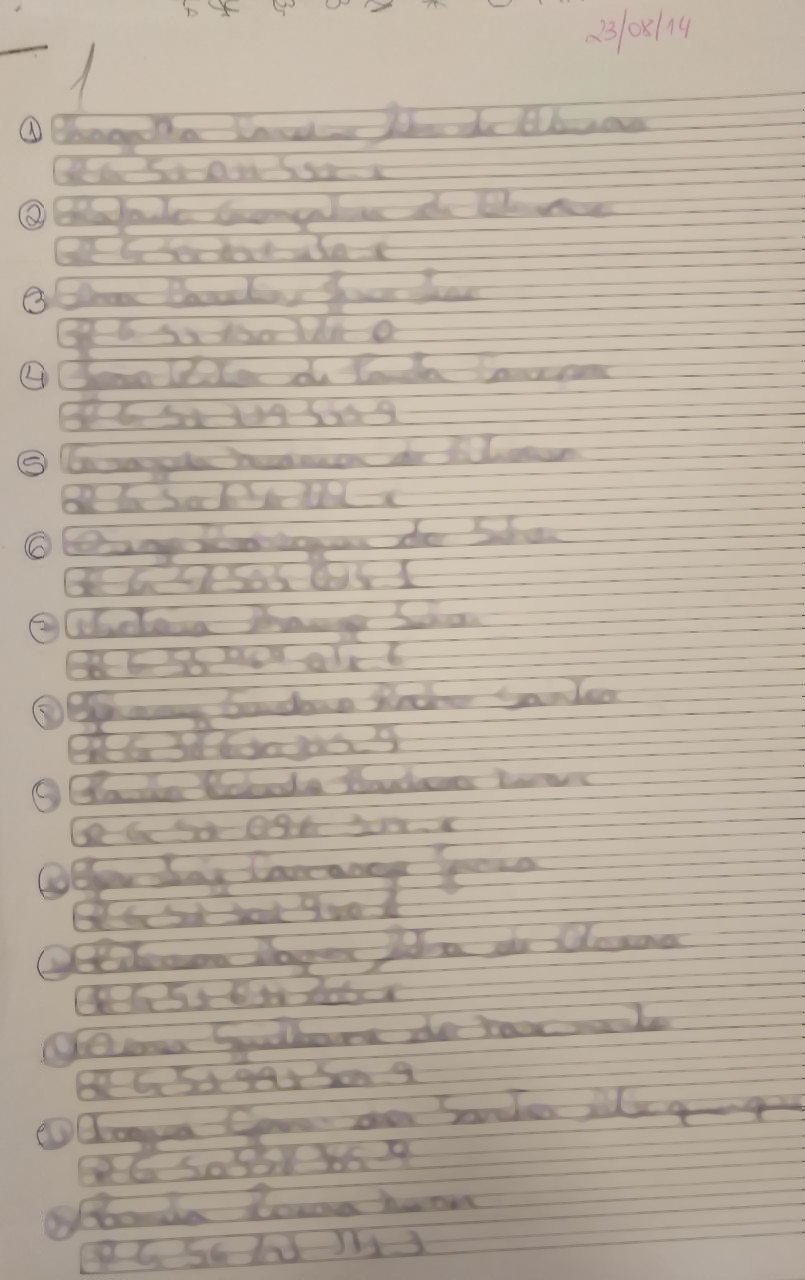
\includegraphics[width=1.0\linewidth]{../../../imagens/blurred-Presenca-Oficina-2014-08-23.jpeg}
                \caption{Testemunhos de presença de estudantes do fundamental, em eventos do Programa WASH, coletados pela autora. O exemplo é de uma oficina em 23 de agosto de 2014. Nos primórdios do Programa eram usados registros na forma de listas de presença em folhas de papel. A imagem foi desfocalizada para proteger a privacidade dos participantes. (fonte: acervo da autora)}
                \label{dec219c809788f521312f8d75d2f5591f069f132}
\end{minipage}%
\hspace{0.5cm}
\begin{minipage}[b]{0.4\linewidth}
        \centering
                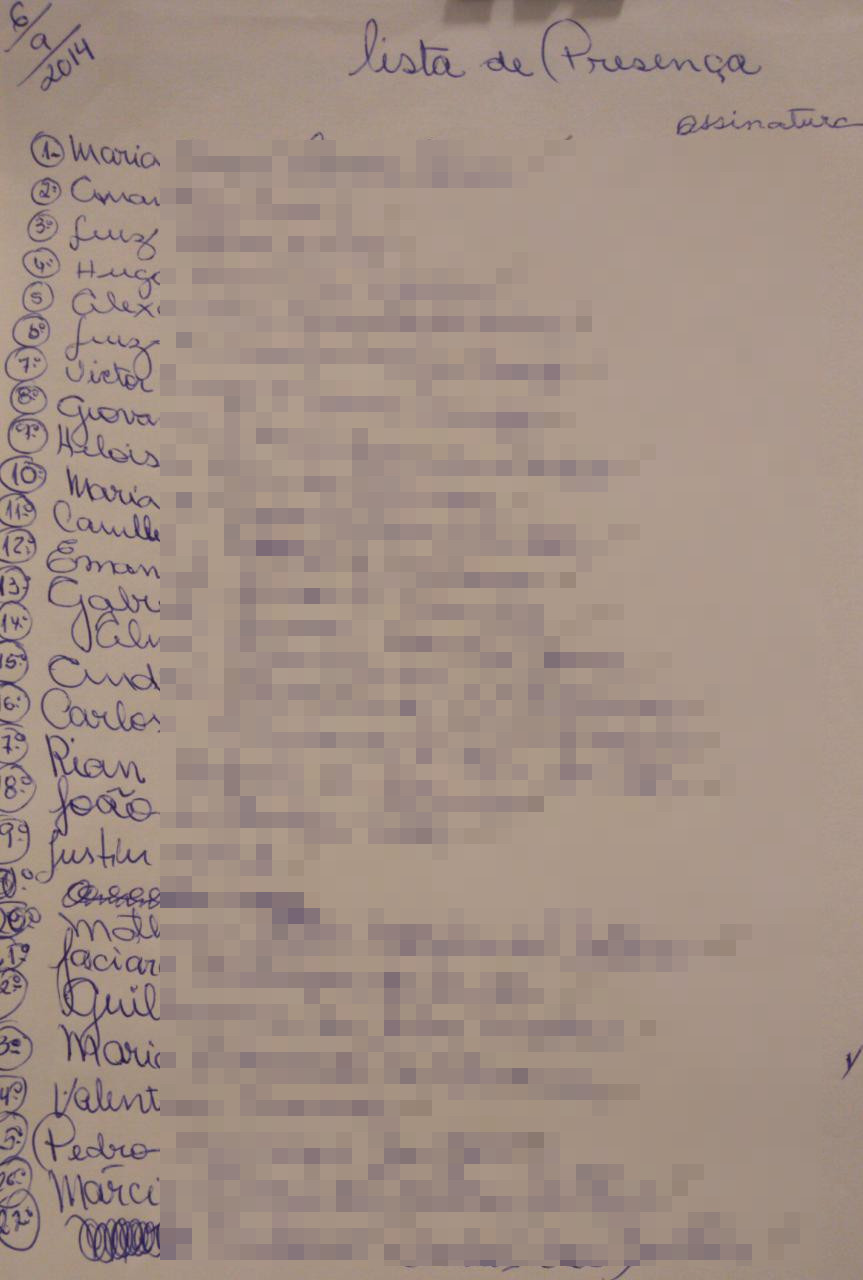
\includegraphics[width=1.0\linewidth]{../../../imagens/blurred-Presenca-Oficina-2014-09-06.jpeg}
                \caption{Exemplo de lista de presença em papel, da oficina realizada em 6 de setembro de 2014. A imagem foi desfocalizada para proteger a privacidade dos participantes. Estes testemunhos eram coletados pela autora para permitir a posterior prestação de contas aos órgãos de fomento. (fonte: acervo da autora)}
                \label{9a8c04c719fc4f9811165547ded35a00eb4fbeed}
\end{minipage}
\hspace{0.5cm}
\begin{minipage}[b]{0.4\linewidth}
        \centering
                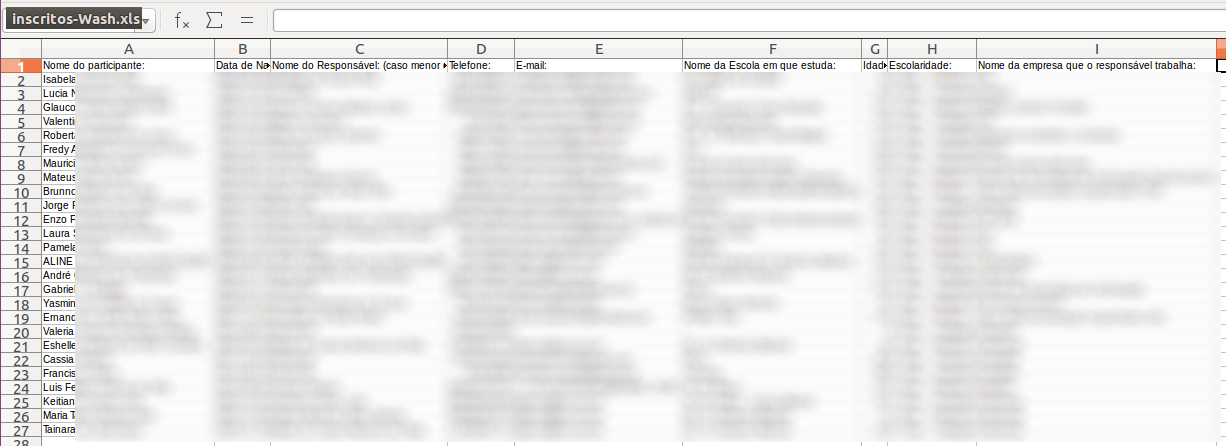
\includegraphics[width=1.0\linewidth]{../../../imagens/blurred-planilha2.png}
                \caption{Planilhas eletrônicas também foram empregadas para armazenar os registros de participações, criando um protocadastro de participantes. A imagem foi desfocalizada intencionalmente para proteger a privacidade dos participantes. (fonte: acervo da autora)}
                \label{b43907f0fa6b6fb935e7384ab03b508859ff0609}
\end{minipage}%
\hspace{0.5cm}
\end{figure}



A Fig. 14 sumariza a evolução do registro de presenças, que se inicia com um manuscrito em folha de papel (2013), passando pelo registro em planilhas eletrônicas (2014) e chegando no uso pleno da plataforma Platuóxe (2022).



\captionsetup{format=plain}
\begin{figure}[htb]

	\begin{center}

		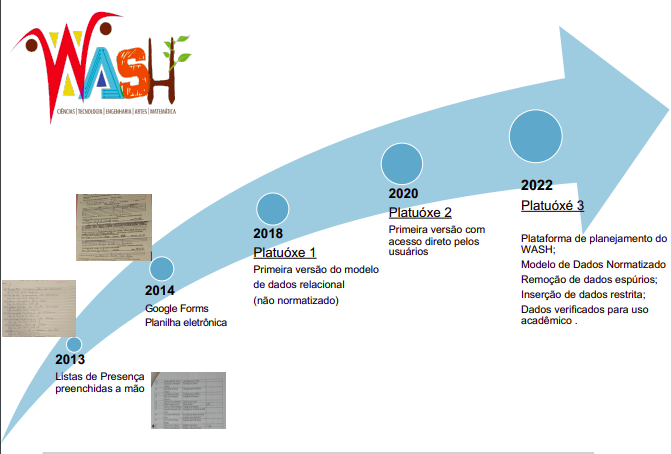
\includegraphics[max size={\textwidth}{\textheight}]{../../../imagens/evolucao-da-documentacao.png}

	\end{center}

	\caption{\label{d237f9364cfe04892cbdffff7fea732012fa5804}Evolução do método de documentação do WASH. (fonte: [[WASHCNPq (2022)]], com participação da autora)}

\end{figure}

Esse cuidado em individualizar os participantes permitia, por exemplo, ter uma melhor noção do perfil etário do público atendido, bem como do interesse das pessoas em participar novamente das atividades, entre tantos outros indicadores que ficarão mais claros no capítulo de Resultados e Análise. Outro aspecto favorável da individualização era uma melhor organização dos documentos do Programa, tais como autorizações para a participação de menores, consentimento de uso de imagem, identificação de responsáveis para casos de emergência, entre outros.

A individualização das presenças era obtida com o registro do nome do participante, o nome do responsável e a data de nascimento. Dessa forma era diminuída a chance de confusão entre homônimos.

Assim, o desenvolvimento da "Platuóxe" nasceu com essa prática inicial de coleta e organização de testemunhos e controle de presença individualizado em oficinas, culminando com a disponibilização do sistema digital de registro.

A primeira versão do Platuóxe permitia registrar as oficinas realizadas, seus participantes e os testemunhos de realização, mas não dispunha de sistema de autenticação de usuário. Por essa razão, requeria que os dados fossem registrados off-line. Mesmo com essa limitação, a primeira versão do software, que ficou pronta no início de 2019, passou a ser usada para gerar os indicadores do programa, de forma rastreável, provendo meios confiáveis de prestar contas aos órgãos de fomento e de controle, viabilizando melhores práticas de "compliance".

A Platuóxe foi sendo evoluída paulatinamente a partir do teste constante de suas funcionalidades, atividade da qual participamos intensamente, juntamente com outros membros do Programa. A cada teste, eram identificados os problemas, com a subsequente propostas de alternativas, que eram implementadas pela equipe responsável pela codificação do Programa. Contribuíram substancialmente para essa fase de desenvolvimento as colegas Clotilde Maffra Diogo e Ana Carolina de Deus Soares.

Com a entrada do desenvolvedor Michel Alencar Morandi, a "Platuóxe" passou a dispor de um sistema de autenticação e todos os participantes do WASH puderam obter suas "contas de usuários do sistema ", descentralizando a entrada de dados.

Não obstante todos os esforços para criar uma ferramenta digital que facilitasse os registros de presença na plataforma, observaram-se muitas oficinas nas quais os registros fotográficos associados indicavam uma presença substancialmente maior do que estava registrado na lista de presença.


\noindent\begin{center}\mbox{\centering\fbox{\centering\par\parbox{0.7\linewidth}{\small\textit{Os dados da Platuóxe representam uma amostra do total de participantes no Programa.}\normalsize}}}\end{center}


Essa situação será discutida no capítulo de Resultados e Análise e está, possivelmente, associada à falta de atribuição legal ao WASH para coletar dados de presença. Com essa limitação, o registro de presença é dependente da ação da entidade responsável, introduzindo uma barreira para dinamizar a coleta de presenças.

\subsection[Modelo relacional de dados do WASH]{Modelo relacional de dados do WASH}\label{Modelo relacional de dados do WASH}
Uma atividade fundamental conduzida pela equipe de codificação da "Platuóxe" foi a modelagem de dados - MD, visando estabelecer as tabelas que seriam necessárias para representar os dados do WASH. Esta modelagem tinha como base as informações fornecidas pelos (as) colaboradores do WASH envolvidos (as) com a operação na ponta, entre eles (as), esta autora.

Como já dito, uma das questões centrais no registro de dados do Programa WASH é saber quem são os(as) seus(suas) participantes. O Programa, por concepção, estimula participações voláteis, dado que as oficinas podem ser abertas e, como prevê o Documento de Referência do WASH, um novo participante consegue acompanhar uma oficina mesmo que não tenha vindo na anterior. Essa volatilidade é uma forma de estimular a inclusão, uma vez que remove barreiras para a participação. Ao mesmo tempo, cria desafios para como os dados serão representados.

No começo da modelagem dos dados, havia uma dúvida sobre se deveríamos criar uma tabela de cadastro para educandos(as), outra para os membros da equipe do WASH e mais outra para os (as) bolsistas (as) multiplicadores (as). A segunda opção seria criar uma tabela única para todos (as) os (as) participantes, independentemente de seu papel no Programa. No caso da criação de uma tabela única, passam a ser necessárias tabela auxiliares, que, de forma coordenada, consigam representar os "tipos de papeis "  desempenhados pelos participantes no WASH.

A segunda opção (tabela única de participantes com tabelas auxiliares) foi a escolhida porque já se antecipava que o WASH seria um programa de longo prazo. Quando o sistema de registro começou a ser elaborado, o WASH já tinha 6 anos e o crescimento anual indicava que haveria fôlego para muitos anos de execução. Assim, não fazia sentido separar os participantes em diversas tabelas, porque era razoável esperar a mudança de papéis dos participantes à medida, que os anos passavam, situação que já era observada em alguns casos, como explicamos a seguir.

De fato, observava-se que educandos do WASH, vinculados ao ensino fundamental, ao adentrar no ensino médio, passavam a realizar sua iniciação científica, mudando de status para bolsistas multiplicadores do Programa. Bolsistas multiplicadores do ensino superior, por sua vez, ao se formarem em seus cursos, mudavam de status, assumindo papéis no  "staff " do WASH; e, assim por diante. Muitos casos de transição de papéis (ou "status ") puderam ser constatados e a ideia de ter múltiplas tabelas para participantes implicaria em um complicado sistema de transição do registro de uma tabela para outra, quando o participante mudasse de papel. Outro motivo para usar uma tabela única para representar participantes é que já se observavam casos de papéis simultâneos, a exemplo de multiplicadores que também eram servidores públicos.

A tabela única de participantes foi denominada "participantes2", sendo parte da  "Platuóxe". Esta tabela está em uso até os dias de hoje sendo complementada por três tabelas auxiliares, que também são partes integrantes da "Platuóxe". A primeira tabela auxiliar é "cargos ", que contém os tipos de vinculação com o WASH. A segunda tabela auxiliar é "instituições ", que contém as instituições a que um participante pode estar vinculado. Para relacionar o participante a um cargo e a uma instituição, foi criada a terceira tabela auxiliar denominada "afiliacoes ", que contém a data de início e do fim daquela afialiação.

Este conjunto de 4 tabelas exemplifica a aplicação do método de modelagem que foi empregado para representar os dados do WASH.

Começaremos mostrando o conteúdo (parcial) da tabela de "cargos", representada na Tabela 6.





\begin{table}[htb]
\tiny
\caption{\label{4d91d8ebc21ea7f9f54231ce125fae7980e789a3}Visão parcial da tabela cargos da base de dados do WASH. A tabela completa tem 42 linhas com registros de cargos.}

\centering
\begin{tabular}{|c|c|}
\hline
id\_chave\_cargo  &  nome\_cargo            \\
             9  &  Coordenador           \\
            10  &  Bolsista EXP A        \\
            11  &  Educando              \\
            13  &  Professor             \\
            15  &  Presidente            \\
            16  &  Diretor               \\
            17  &  Servidor              \\
            18  &  Coordenador Local     \\
            19  &  Coordenador Nacional  \\
            21  &  Deputado              \\
            22  &  Presidente            \\
            23  &  Multiplicador         \\
            25  &  Bolsista PCI   \\
            26  &  Bolsista ITI A \\
            27  &  Bolsista ITI B \\
            28  &  Reitor \\
            31  &  Secretaria \\
            38  &  Prefeito              \\
            39  &  Pesquisador           \\
            40  &  Secretaria Executiva             \\
            42  &  Estudante    \\
            43  &  Estagiario \\
            48  &  Bolsista EXP B \\
            49  &  Bolsista EXP C \\
            50  &  Bolsista ATP B \\
            51  &  Educando \\
            52  &  Voluntario \\
            54  &  Orientador            \\
            55  &  Bolsista DTI A \\
\hline
\end{tabular}
\end{table}


Na sequência, mostramos uma visão parcial da tabela "Instituicoes" (ver Tabela 7), que contém todas as instituições atendidas pelo WASH. A tabela completa tem 150 linhas de registros de instituições, mas estamos mostrando apenas 38, por motivos de espaço.





\begin{table}[htb]
\tiny
\caption{\label{025a2a6fc8be57e0e8305d2e65ad8cc8f02f2308}Visão parcial da tabela instituicoes da base de dados do WASH. A tabela completa tem 150 linhas com registros, de instituições. Na presente reprodução foram selecionados registros que mostram a pluralidade do atendimento do WASH, tendo sido retirados as repetições de tipos de instituições por motivos de espaço.}

\centering
\begin{tabular}{|c|c|}
\hline
id\_chave\_instituicao  &  nome\_instituicao \\
                  164  &  APAE  \\
                   68  &  Associação Cultural Bola de Meia \\
                   74  &  Biblioteca Cidadã Paulo Freire  \\
                   52  &  Camara Federal \\
                   32  &  Câmara Municipal de Campinas                                                      \\
                   25  &  Casa de Cultura Taina                                                             \\
                  168  &  CEI Vovó Maria                                                                    \\
                   23  &  Cemaden                                                                           \\
                  150  &  Centro de Formação Popular Frei Betto                                             \\
                   19  &  Centro Paula Souza                                                                \\
                   22  &  Ciência em Show                                                                   \\
                   57  &  CNPq                                                                              \\
                   91  &  Colégio Estadual Rio Branco                                                       \\
                   56  &  CPqD                                                                              \\
                    1  &  CTI Renato Archer                                                                 \\
                   70  &  E.E. Vitor Meireles                                                               \\
                   80  &  E.E. Expedito Camargo Freire                                                      \\
                  130  &  EMEF Décio Moreira \\
                    5  &  Escola Dona Lindu \\
                  128  &  Escola Estadual MAJOR MIGUEL NAKED \\
                  111  &  ETEC Carapicuíba \\
                   47  &  Exército Brasileiro \\
                  156  &  Faculdade Zumbi dos Palmares \\
                   53  &  FAPESP \\
                  119  &  Fundação Araucária \\
                   35  &  Governo do Estado de São Paulo \\
                  127  &  IFPR - Campus Pitanga \\
                   62  &  PUC de Campinas \\
                   21  &  Prefeitura de São Paulo           \\
                   48  &  Bolsista EXP \\
                   49  &  Secretaria de Cultura de Londrina \\
                   85  &  Secretaria de Educação de Jacareí/SP \\
                  169  &  SENAC Minas  \\
                   38  &  Sindicato dos Metalúrgicos do ABC \\
                   16  &  Unicamp \\
                   75  &  UNIFESP  \\
                    9  &  USP \\
                  181  &  UTFPR \\
\hline
\end{tabular}
\end{table}


Para dar prosseguimento à exemplificação, agora isolaremos um participante do Programa, separando seu registro do resto da tabela "participantes2" (ver Tabela 8). Note que a tabela original (participantes2)  tem 3312 registros, (linhas) mas decidimos usar como exemplo um único participante, resultando em apenas uma linha na Tabela 8. Substituímos o nome do participante para proteger sua privacidade, substituindo-o por um nome fictício ("Maria Pereira ").





\begin{table}[htb]
\tiny
\caption{\label{96081f1bc28f7c738012f4beb3ef867b6b67107f}Exemplo de linha da tabela participantes2, selecionada para que se possa entender como o registro dos papéis desempenhados por cada participante é feito no âmbito do WASH. A tabela participantes2 tem 3312 registros de participantes.}

\centering
\begin{tabular}{|c|c|c|}
\hline
id\_chave\_participante  &  nome\_participante             &  data\_nascimento  \\
                     2  &  Maria Pereira  &  1994-06-15 \\
\hline
\end{tabular}
\end{table}


É importante observar, na última coluna da Tabela 8 que, por escolha da área de TI do WASH, todas as datas no âmbito dos registros do Programa são invertidas, sempre começando pelo ano, passando pelo mês e terminando no dia. Isto é feito assim para garantir que a ordenação dos registros por data seja facilitada.

Agora, vamos extrair da tabela "afiliacoes", (ver Tabela 9) todos os registros cujo identificador de participante seja "2 ", como consta no excerto da tabela participantes2 mostrado na Tabela 8.





\begin{table}[htb]
\tiny
\caption{\label{22b8f800790bcad960b91cc2a9e7f073a4a20b8f}Subconjunto de registro da tabela afiliacoes, onde foram selecionados apenas os dados do participante que tem identificador 2 na tabela participantes2.}

\centering
\begin{tabular}{|c|c|c|c|c|c|}
\hline
id\_participante  &  id\_instituicao  &  id\_cargo  &  nome\_documento  &  inicio      &  fim \\
              2  &              62  &        42  &  RA12345679      &  2012-02-01  &  2015-01-31  \\
              2  &              57  &        48  &  111111/2018-9   &  2018-08-01  &  2019-07-31  \\
              2  &              57  &        48  &  222222/2019-6   &  2019-08-01  &  2019-12-31  \\
              2  &              57  &        48  &  333333/2019-2   &  2020-08-01  &  2021-12-31  \\
              2  &              57  &        26  &  444444/2016-1   &  2016-08-02  &  2017-07-31  \\
              2  &              62  &        52  &  não consta      &  2015-08-01  &  2016-08-01 \\
\hline
\end{tabular}
\end{table}


O excerto da tabela "afiliacoes" mostrado na tabela 9 indica que a participante identificada pelo número 2 (Maria Pereira)  teve duas afiliações durante o período em que esteve vinculada ao WASH: à universidade PUC de Campinas, que é identificada pelo número 62 e ao CNPq, que é identificado pelo número 57 (se tiver dúvida, veja o identificador dessas instituições na Tabela 7).

Além disso, essa mesma participante identificada pelo número 2 desempenhou 4 papéis no WASH (ver Tabela 6): estudante, identificado pelo número 42, Bolsista EXP B, identificado pelo número 48 e Bolsista ITI A, identificado pelo número 26.

A tabela "afiliacoes" também permite conhecer o documento que formaliza a vinculação com o Programa WASH, pelo campo nome\_documento (ver Tabela 9). Os campos "inicio " e "fim " permitem conhecer o período em que uma determinada afiliação estava válida.

O exemplo mostrado até agora permite compreender o método baseado em bancos de dados relacionais de uma forma prática.

O sistema de armazenamento de dados do WASH é integralmente baseado nessa lógica de múltiplas tabelas, que se relacionam por meio de identificadores numéricos. Esse método é bastante robusto e reduz sobremaneira a ocorrência de dados espúrios, muito embora ainda exista a possibilidade de algum erro estar presente, porque a integridade da base de dado é dependente da qualidade do preenchimento de dados. Isso quer dizer que, para garantir a qualidade de dados, é preciso uma capacitação constante dos colaboradores.

A maior robustez do método relacional vem justamente do fato de que a informação está segregada, de forma que em cada tabela exista apenas um registro para cada fato representado. Em outras palavras: note que na tabela "participantes2" (ver Tabela 2) existirá apenas 1 registro para o participante que é identificado pelo número 2 (Maria Pereira), ao passo que na tabela "cargos " (ver Tabela 6) haverá apenas um registro identificado pelo número 48 (Bolsista EXP B), da mesma forma que na tabela "instituicoes " (ver Tabela 7) haverá apenas um registro identificado pelo número 57 (CNPq).

Vimos que o participante identificado pelo número "2 " teve  pelo menos 6 diferentes tipos de vínculos com o WASH, em momentos diferentes de sua atuação, mas não foi preciso criar 6 registros na tabela "participantes2". Se o WASH usasse planilhas eletrônicas para guardar seus dados seria necessário repetir 6 vezes todas as informações sobre o participante, criando a oportunidade para falta de uniformização de dados e, portanto, perda de confiabilidade nos mesmos.

Para representar todos os seus dados de forma flexível e adaptável às suas diversas parcerias, o sistema de armazenamento de dados do WASH precisou criar 54 tabelas, como mostrado na Tabela 10.





\begin{table}[htb]
\tiny
\caption{\label{5b2e4ba8f3836249e7dd88b37344da7bfa3669c5}O banco de dados relacional da Platuóxe é constituído por 54 tabelas}

\centering
\begin{tabular}{|c|c|}
\hline
afiliacoes                     &   local\_eventos \\
 atividades                     &   local\_part \\
 atividades\_eventos             &   modelo\_atividades\_eventos \\
 atividades\_fotos               &   modelo\_documentos\_eventos \\
 avaliacao\_bolsista             &   modelo\_eventos \\
 bolsa\_cnpq                     &   modelo\_tematicas\_eventos \\
 cargos                         &   parametros \\
 comentario\_evento              &   part\_eventos \\
 compartilhados                 &   participantes2 \\
 documentos                     &   processo\_cnpq \\
 documentos\_equipes             &   processo\_ivan\_valente \\
 documentos\_eventos             &   processo\_wash\_ABC \\
 documentos\_instituicoes        &   processo\_wash\_cury \\
 documentos\_participantes       &   processo\_wash\_regioes \\
 estimativa                     &   relacao\_grupo\_modelo \\
 eventos                        &   responsaveis\_eventos \\
 fontes                         &   status \\
 fontes\_eventos                 &   status\_doc \\
 formacao                       &   tematicas \\
 fotos                          &   tematicas\_eventos \\
 grupo\_evento                   &   tipo\_documento \\
 grupo\_modelo                   &   tipos\_encerramento \\
 grupo\_participante             &   trash \\
 grupos                         &   trash\_fontes \\
 inst\_eventos                   &   trash\_fotos \\
 instituicoes                   &   vincula\_instituicao\_instituicao \\
 locais                         &   vincula\_local\_instituicao \\
\hline
\end{tabular}
\end{table}


Não aprofundaremos mais na descrição da modelagem de dados do Platuóxe por razões de espaço, mas acreditamos que as informações até agora compartilhadas permitem ao leitor compreender o método de registro de dados utilizado nesta dissertação.

\subsection[Consulta à base de dados através da Linguagem SQL]{Consulta à base de dados através da Linguagem SQL}\label{Consulta à base de dados através da Linguagem SQL}
Vimos no capítulo de Fundamentação Teórica um rápida descrição dos princípios da Linguagem SQL.1

Essa linguagem foi extensamente utilizada como método para obter os indicadores deste Projeto. Para isso, foi aplicada à base de dados relacional da plataforma Platuóxe descrita na seção anterior.

As consultas SQL foram elaboradas pela equipe de TI, com base nas especificações dos indicadores de interesse para esta autora. Em algumas situações, os resultados dessas consultas puderam ser verificados pelo emprego de uma planilha eletrônica, elaborada pela autora.

\subsection[Método de determinação do sexo dos participantes]{Método de determinação do sexo dos participantes}\label{Método de determinação do sexo dos participantes}
A maior prevalência de participação masculina em atividades STEAM, em detrimento da feminina, é um fenômeno que, infelizmente, se reproduz mundialmente (KIJIMA et al., 2021). Cabe ao WASH verificar, da melhor forma possível, se essa situação injusta está sendo reproduzida dentro do próprio Programa, com vistas a promover intervenções que possam mitigá-la.

Com a finalidade de verificar essa situação, decidimos incluir, entre os indicadores do Programa, o percentual de mulheres e homens participantes. Isso exigiu um esforço de criação de um método especial, uma vez, que antes de 2019 o WASH não armazenava dados de sexo ou gênero.

É possível identificar vários estágios, ao longo da existência do WASH, referentes à forma de armazenar dados (ver Fig. 14). Foi comentando na seção anterior que logo no início do Programa, por exemplo, os dados de participantes eram coletados por meio de listas de presença em papel (ver Figs. 11, 12 e 13). Estas listas registravam apenas o nome dos participantes e a data do evento, sem registro de sexo. Posteriormente, novos dados foram sendo coletados, como o ano do nascimento da criança, seu Registro Geral (RG) ou do responsável, mas ainda sem registrar o sexo.

1Esse crescimento gradativo na quantidade de dados coletados revela, por parte da Coordenação do WASH, um cuidado de armazenar exclusivamente dados que estavam vinculados aos objetivos do Programa. Essa visão decorre do Programa não ter um mandato específico (atribuição legal) para registro de dados cadastrais mais detalhados. Na falta desse mandato, o registro sem propósito desses dados pode ser considerado prejudicial à privacidade dos participantes, requerendo custosas medidas de proteção de dados adicionais.

Assim, é possível compreender porque a coleta de dados sempre foi mantida no limite dos propósitos do projeto, a saber: contabilizar o número de participantes, evitar a contagem duplicada de participantes, identificar os responsáveis para o caso de emergências, registrar autorizações de uso de imagens, e assim por diante.

Em outras palavras, por falta de conexão com os objetivos iniciais do Programa, não havia armazenagem de dados de sexo de seus participantes.

Com o passar dos anos, percebeu-se que o projeto já contava com milhares de cadastros incompletos, comprometendo a avaliação equânime do Programa mencionada no começo desta seção.

Para vencer essa deficiência de cadastro, decidiu-se por criar um método em que os indicadores de sexo do WASH pudessem ser construídos a partir de uma avaliação a posteriori (em relação ao momento do cadastro) dos primeiros nomes dos participantes. Esse método pode ser sumarizado como:


\noindent\begin{center}\mbox{\centering\fbox{\centering\par\parbox{0.7\linewidth}{\small\textit{O método consiste em verificar se o primeiro nome de cada participante está numa lista extensiva de nomes "considerados masculinos", situação em que, de forma anonimizada, um contador de participantes masculinos é incrementado. Caso o primeiro nome do participante esteja numa lista de nomes "considerados femininos", o contador de participantes femininos é incrementado. Quando o nome não está em nenhuma das listas ou quando é um nome com sexo indefinido, o contador de "sexo desconhecido" é incrementado.}\normalsize}}}\end{center}


A rigor, do ponto de vista do WASH, não há interesse em rotular peremptoriamente as pessoas com base no sexo identificado por esse método. Por essa razão, o dado de sexo gerado não é vinculado ao cadastro do participante, ficando armazenado num contador anonimizado.

Dito isso, o fato é que o primeiro nome do participante não permite avaliar a identidade de gênero. Assim, a postura limita a coleta de dados gerando uma reconhecida deficiência de registro associada à falta de coleta de dados autodeclaratórios de gênero antes de 2019.

Mesmo reconhecida esta deficiência, os números encontrados (ver Resultados e Análise) indicam que a estimativa produzida pelo método é suficiente para suportar a avaliação das hipóteses desse trabalho.

\chapter[RESULTADOS E ANÁLISES]{RESULTADOS E ANÁLISES}\label{RESULTADOS E ANÁLISES}
Alcançamos o final dos caminhos percorridos (métodos) descritos no capítulo anterior, criando as condições para que os resultados obtidos sejam apresentados.

Os resultados obtidos serão descritos e, concomitantemente, analisados para que a validade das hipóteses levantadas possa ser verificada.

Os resultados estão organizados, inicialmente, em duas seções separadas, relacionadas aos eixos da da presente pesquisa:


\begin{itemize}
\item história (eixo 1)
\item indicadores (eixo 2); e
\end{itemize}

Será apresentada uma terceira seção contendo uma síntese que integrará os achados dos dois eixos indicados acima. Esta terceira seção analisará cada hipótese separadamente.

\section[Narrativas contruídas a partir do método historiográfico (eixo 1)]{Narrativas contruídas a partir do método historiográfico (eixo 1)}\label{Narrativas contruídas a partir do método historiográfico (eixo 1)}
Aqui, são apresentadas as narrativas construídas a partir da aplicação do método historiográfico, descrito em Materiais e Métodos.

O método utilizado se baseia na análise do acervo de documentos oficiais (portarias, planos de trabalho, termos de outorga, boletins, legislação, entre outros), registros pessoais da autora (fotografias, vídeos, diários, entre outros) e literatura (artigos, notícias, entre outros), complementados pelas memórias narradas pelos partícipes do percurso histórico em estudo. Estas memórias foram colhidas pela autora por meio de entrevistas.

Como já indicado no Capítulo de Materiais e Métodos, no texto final da narrativa histórica, buscamos intercalar conhecimentos obtidos do acervo com trechos selecionados das entrevistas citadas, complementando o olhar objetivo da autora com a subjetividade dos atores entrevistados.

\subsection[O GESAC e sua contribuição para  a cultura  digital  no país]{O GESAC e sua contribuição para  a cultura  digital  no país}\label{O GESAC e sua contribuição para  a cultura  digital  no país}
Vimos na Introdução que os benefícios e conforto trazidos para os dias de hoje por esse admirável mundo novo digital são resultados de ações e iniciativas da ciência e da tecnologia, que foram deflagradas lá nos anos 50, impulsionadas ao longo das décadas seguintes, mas cuja popularização e disseminação se intensificaram nos anos 90.

Os anos 90 são considerados como os anos dourados para que chegássemos à atual configuração de planeta tecnológico e informatizado, que vivencia a Sociedade da Informação em suas várias dimensões. Esta afirmação se sustenta na consolidação das cadeias produtivas, que permitiram reduzir o custo dos equipamentos digitais e sua consequente difusão (CIPOLI, 2012), preparando o mundo para o crescimento do acesso às redes digitais observado na década seguinte, como exemplificado na Fig. 1, em que é mostrado o crescimento do acesso à internet no Brasil.

Dentre os  inúmeros feitos dessa época, basta lembrarmos o surgimento da Internet, a popularização do computador pessoal e a chegada dos dispositivos móveis (celulares).

Na esfera governamental, o Brasil assistiu, a partir de 2003, bem no início do Governo Lula, a implantação do Governo Eletrônico e Serviço de Atendimento ao Cidadão- GESAC.

Mas, o Programa tinha sido instituído oficialmente um ano antes, pelo Ministério das Comunicações do Governo FHC, por meio  da Portaria nº. 256, de 13 de março de 2002 (BRASIL, 2004), cujo  objetivo era disseminar meios que permitissem a universalização do acesso às informações e serviços do governo, por meio eletrônico no território nacional, a toda população brasileira (BRASIL, 2002).

A licitação para a contratação de uma empresa para implantação do Programa GESAC foi realizada durante o governo FHC, no ano de 2002. Na época, foram alocados para o Programa GESAC recursos da ordem de 86 milhões de reais para serem investidos ao longo de 18 meses.

Antônio Albuquerque, entrevistado pela autora e primeiro Diretor Nacional do GESAC, traz uma visão esclarecedora do que previa a proposta de 2002:


\noindent\begin{center}\mbox{\centering\fbox{\centering\par\parbox{0.7\linewidth}{\small\textit{"A proposta do GESAC, originalmente estabelecida no Governo FHC, tinha algumas deficiências. Por exemplo, o GESAC original previa apenas instalação de infraestrutura para permitir o acesso a sites do governo, sem nenhuma apropriação tecnológica por parte das comunidades. Outra deficiência era escolha dos locais de instalação dos pontos de presença, que seria feita pela empresa contratada, sem uma articulação para identificar onde realmente estavam as pessoas mais necessitadas. Outro problema era a tímida abrangência prevista para o programa, que com poucos milhares de computadores planejados, não contemplava o desafio de levar inclusão digital para um país continental como o Brasil. Em suma, o Programa GESAC, como estava especificado no processo licitatório de 2002, estava muito aquém do que deveria ser um verdadeiro Programa de inclusão digital." (fonte: entrevista com Antônio Albuquerque, Diretor Nacional do Programa GESAC em 2003)}\normalsize}}}\end{center}


O entendimento manifesto pela Coordenação do Relacionamento com as Comunidades do Programa GESAC, Toni Klaus, também entrevistado por esta autora, corrobora com a visão trazida por Antônio Albuquerque, acrescentando que a proposta de 2002, embora licitada, nunca fora colocada em prática:


\noindent\begin{center}\mbox{\centering\fbox{\centering\par\parbox{0.7\linewidth}{\small\textit{"Para se falar do GESAC , eu entendo que temos que situá-lo no tempo. O Governo Lula estava começando em 2003 e a internet estava em amplo processo de popularização no Brasil e no mundo, desde 1996. O GESAC foi uma iniciativa do governo FHC, que nunca tinha sido executada. A iniciativa original previa 1200 Pontos de Presença, para serem disponibilizados em lugares públicos, tais como quiosques para acesso à internet pela população, em postos dos correios e outras localizações semelhantes. Mas, esse contrato nunca foi executado no âmbito do governo FHC." (fonte: entrevista com Toni Klaus Bochat,Programa GESAC entre 2003 e 2005)}\normalsize}}}\end{center}


O implementador do GESAC, Angel Luis, sintetiza as duas visões sobre a proposta de 2002 com a metáfora de "Guichê Eletrônico":


\noindent\begin{center}\mbox{\centering\fbox{\centering\par\parbox{0.7\linewidth}{\small\textit{"O Programa tinha a finalidade inicial (em 2002) de ser o "guichê eletrônico" do governo federal." (fonte: entrevista com o implementador do GESAC, Angel Luis)}\normalsize}}}\end{center}


Foi durante o ano de 2003, no primeiro Governo Lula, que de fato iniciou-se o funcionamento do  GESAC. Os gestores que assumiram a responsabilidade pelo Programa usaram o primeiro semestre de 2003 para que se fizessem as adequações administrativas e técnicas necessárias para transformá-lo em um amplo processo de inclusão digital. Essas adequações foram resultado de mudanças conceituais no Programa GESAC com alterações de seus princípios, colocando seus beneficiários como protagonistas do processo de inclusão digital.

No segundo semestre de 2003, o Programa GESAC foi efetivamente implantado com os Pontos de Presença (PPs), espaço com  computadores conectados à internet, via satélite. À época, cada PP deveria ter, no mínimo, entre cinco e quinze computadores, podendo ser utilizados gratuitamente por cada comunidade local.

Com a readequação do Programa GESAC, foi criado o Departamento de Inclusão Digital - DESID, no Ministério das Comunicações, sendo nomeado como diretor, Antônio Bezerra de Albuquerque, que conduziu a implantação e gestão do GESAC. Posteriormente esse executivo, veio a contribuir também com o Programa WASH.


\noindent\begin{center}\mbox{\centering\fbox{\centering\par\parbox{0.7\linewidth}{\small\textit{"No inicio de 2003, o engenheiro Antônio Albuquerque, funcionário de carreira do CPqD da Telebrás da cidade de Campinas, é designado  assessor especial do Ministro das Comunicações. Uma  de suas tarefas foi analisar o contrato do GESAC e, se necessário, fazer as adequações contratuais, atendendo às novas diretrizes de inclusão digital do governo federal. Foi adotado o uso do software livre e disponibilizado um data-center com um conjunto de ferramentas destinadas aos usuários  para a produção de conteúdos e suporte operacional." (fonte: entrevista com Toni Klaus Bochat, Programa GESAC entre 2003 e 2009)}\normalsize}}}\end{center}


O primeiro Ponto de Presença - PP foi  instalado na  Escola Estadual Belmiro Soares, na cidade de Paranaguaiara, em  Goiás.

As diretrizes de política pública de inclusão digital que o GESAC procurou atender, a partir de 2003 foram:


\begin{itemize}
\item oferecer acesso aos serviços de governo eletrônico (e-gov);
\item acesso à internet deveria ser irrestrito;
\item oferecer conexão de banda larga, via satélite (ver antena GESAC na Fig. 15), para atender às comunidades sem infraestrutura,  em localidades distantes, que não poderiam ter acesso a esse serviço;
\item implantar uso e gestão comunitária dos equipamentos, possibilitando a apropriação coletiva  da tecnologia,  desenvolvimento local através de apoio à produção econômica, educativa e cultural da comunidade;
\item oferecer uma cesta de serviços on-line de apoio ao usuário para o processo de inclusão digital, disponibilizando correio eletrônico (e-mail),  jornal mural (Teia), sistema de compartilhamento de informações ( RAU-TU) e hospedagem de sítios eletrônicos produzidos pela comunidade (Pousada). Todos os serviços  foram oferecidos em software livre, conforme as diretrizes do governo da época;
\item criação do portal IDBRASIL para estabelecer um canal de comunicação entre o MC e as comunidades e entre as próprias comunidades. Esse portal dava acesso aos serviços do programa e ao compartilhamento  de informações  entre as comunidades usuárias;
\item promover a apropriação das TICS  para as comunidades usuárias, por meio de  capacitações e oficinas de formação de multiplicadores.
\item Disponibilização de uma plataforma multisserviços com voz sobre ip, serviço 0800, 700 mil caixas postais de e-mail, espaços para produção de “homepages”, canal de IP-TV, multicasting, oficinas de cultura digital, encontros de formação e outros;
\end{itemize}



\captionsetup{format=plain}
\begin{figure}[htb]

	\begin{center}

		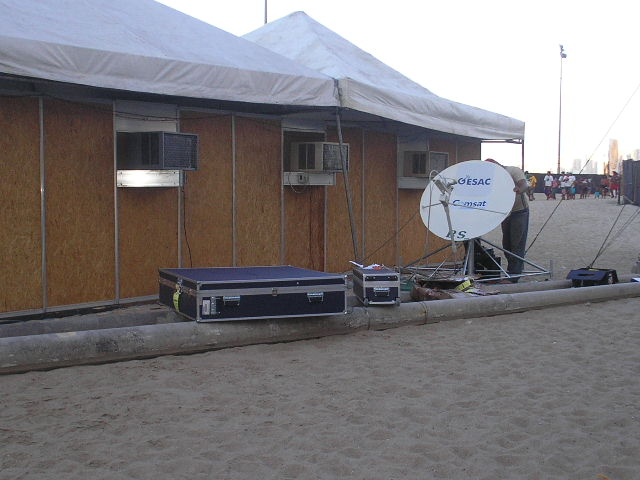
\includegraphics[max size={\textwidth}{\textheight}]{../../../imagens/antenagesac.jpg}

	\end{center}

	\caption{\label{a3225c07ca3bc896130a8519e74f575fb919fefd}Antena Gesac, instalada nos jogos indígenas.}

\end{figure}

Tinha-se a compreensão que somente a disponibilização de equipamentos tecnológicos não era suficiente, mas  era imprescindível que o Programa contribuísse para a formação dos usuários no uso das tecnologias de informação e comunicação. Em 2004, passou-se a oferecer oficinas de capacitação,em campo, às comunidades através de profissionais denominados como implementadores sociais, pessoas com habilidades técnicas,  que realizavam o trabalho de formação  e apropriação das TICS pelas comunidades.

O grupo de implementadores(as) sociais passou por um processo de seleção e formação sobre o Programa. A escolha buscava identificar habilidades técnicas e sociais, com vistas à atuação em diversas comunidades. Para garantir pluralidade, os implementadores (as) eram oriundos(as) de todas as regiões do Brasil. A formação destes (as) implementadores (as) buscava  permitir que eles (elas) aprendessem, dominassem, compartilhassem  e disseminassem a utilização dos serviços oferecidos pelo GESAC, assim como a adoção e o uso de software livre. Essas pessoas visitavam as comunidades de Norte a Sul do país, preparando e realizando oficinas, e fazendo a migração para o uso do software livre. O Programa GESAC seguia as Diretrizes, Objetivos e Ações prioritárias para implementar o uso do Software Livre, conforme estabelecido no Planejamento Estratégico 2003-2004, organizado pela  Casa Civil, Presidência República, em que essa autora fez parte do Comitê Técnico de implementação do Software Livre.

Entre as atividades que deveriam realizar estavam:


\begin{itemize}
\item instalação de laboratórios (as atividades incluíam, por exemplo, a capacitação em cabeamento de rede, migração de softwares proprietários para software livre, dentre outras atividades técnicas)
\item promoção de encontros locais e estaduais do programa,
\item colaboração para que os  Pontos de Presença organizassem o seu comitê de gestor,
\item resolução ou encaminhamento de possíveis questões técnicas.
\end{itemize}

A cada implementador (a) era disponibilizado um equipamento GPS, celular, notebook, projetor multimídia e kit de ferramentas. O papel mais visível das pessoas que atuavam na condição de implementadores (as) era o de oferecer as oficinas de cultura digital, bem como colaborar para que a as pessoas inseridas em suas comunidades tivessem acesso e pudessem se apropriar das tecnologias da informação e comunicação que estavam sendo disponibilizadas.


\noindent\begin{center}\mbox{\centering\fbox{\centering\par\parbox{0.7\linewidth}{\small\textit{"Os implementadores sociais trabalhavam localmente nos pontos implantados, principalmente com os administradores desses pontos. A ideia era multiplicar os conhecimentos do mundo digital para os usuários locais. Eram feitas oficinas sobre os serviços disponibilizados pelo GESAC, mas também sobre Software Livre em geral (ver Figs. 17 e 18)). O uso de software livre era uma política pública do governo federal e, portanto, todos os computadores do programa tinham uma distribuição em software livre. Os serviços disponibilizados também eram em software livre." (fonte: entrevista com Toni Klaus Bochat, do Programa GESAC entre 2003 e 2009)}\normalsize}}}\end{center}


A  primeira geração de implementadores  sociais foi composta por:


\begin{itemize}
\item Rafael Gomes da Cruz (Banto Palmarino) (ver Fig. 16);
\item Victor Reis;
\item Angel Luís;
\item Tatiane Wells;
\item Isabela Toya;
\item Sergio Melo;
\item Renata Lourenço;
\item Eduardo Aguiar;
\item Vincenzo Tozzi (ver Fig. 19)
\end{itemize}

Após 20, colhemos as impressões de uma parte dos(as) implementadores(as) sobre o que aquele Programa significou em suas vidas, um elemento que consideramos importante para nosso processo historiográfico, razão pela qual registramos  o relato de três entrevistados (as): Sérgio Melo, Renata Lourenço e Angel Luis.


\noindent\begin{center}\mbox{\centering\fbox{\centering\par\parbox{0.7\linewidth}{\small\textit{"Ter feito parte da equipe de implementadores  sociais do GESAC foi  de extrema relevância para a minha vida, quando tive a oportunidade de conviver com tantas pessoas, em tantos lugares, e contextos sociais diferentes. Isso me fez perceber e vivenciar na prática toda a multiplicidade  de saberes, culturas, experiências e, também, as dificuldades que fazem parte da  constituição social do nosso país." (fonte: entrevista com Sérgio Melo, implementador do  GESAC, entre, 2003 e 2005)}\normalsize}}}\end{center}



\noindent\begin{center}\mbox{\centering\fbox{\centering\par\parbox{0.7\linewidth}{\small\textit{"Foi uma primeira experiência profissional que me colocou no mercado de trabalho, de uma forma muito positiva. O GESAC contribuiu para que eu me reconhecesse neste mundo enquanto  pessoa negra, pessoa indígena, enquanto jornalista, com as potencialidades que essa profissão oferece no campo da comunicação." (fonte: entrevista com Renata Lourenço)}\normalsize}}}\end{center}



\noindent\begin{center}\mbox{\centering\fbox{\centering\par\parbox{0.7\linewidth}{\small\textit{"Quando eu fui convidado para integrar o Gesac me propuseram a realização de oficinas de produção audiovisual, a promoção do jornalismo comunitário e de debates sobre o papel da mídia. A promoção do ativismo cidadão era parte da minha vida, mas a "militância hacker", ainda não. Álvaro Malaguti, que me fez o convite, perguntou: "Você sabe mexer com Linux? ",  respondi "Não, mas aprendo!". (fonte: entrevista com Angel Luis, implementador do GESAC, entre 2003 e 2005)}\normalsize}}}\end{center}


Os implementadores (as) percorreram os Pontos de Presença, GESAC instalados em comunidades urbanas, rurais, quilombolas, indígenas, ribeirinhos, sem-terra, telecentros, pontos de cultura, escolas, sindicatos, entre outros, ensinando e aprendendo. Eles planejavam seus trabalhos e as visitas nas comunidades usando uma ferramenta de edição colaborativa (Wiki). Mensalmente, cada implementador apresentava seu relatórios de atividades. Escolhemos um trecho da entrevista de Sérgio Melo para ilustrar essa presença em lugares remotos, que segue.


\noindent\begin{center}\mbox{\centering\fbox{\centering\par\parbox{0.7\linewidth}{\small\textit{"Do ponto de vista das comunidades  atendidas e dos impactos gerados, eu avalio que o GESAC esteve presente num momento determinante da história da tecnologia no Brasil. Um momento em que o acesso tanto aos equipamentos eram muitos restritos, o acesso a internet também era ainda bastante embrionário e o GESAC transgredia essa regra ao levar conectividade a contextos tão diversos e lugares tão afastados dos grandes centros urbanos, quanto, também, pela disponibilização dos equipamentos que eram tão fundamentais para que o Programa desse certo." (fonte: entrevista com Sérgio Melo, implementador do GESAC, entre 2003 e 2005).}\normalsize}}}\end{center}


Sobre os universos quilombola e indígena, tivemos a oportunidade de coletar as impressões do entrevistado Antônio Carlos (TC) Santos Silva, líder comunitário da Casa de Cultura Tainã, um quilombo urbano localizado na cidade de Campinas que, com apoio do GESAC, conseguiu estabelecer a conexão digital de quilombos espalhados pelo país. Essa iniciativa ficou conhecida como Rede Mocambos.


\noindent\begin{center}\mbox{\centering\fbox{\centering\par\parbox{0.7\linewidth}{\small\textit{"A Rede Mocambos se expandiu para o território nacional quando nasceu o convênio com o poder público, através do GESAC, em 2007. Mas, a ideia de redes quilombolas e indígenas conectadas surgiram muito antes. Foi essa estruturação anterior que permitiu à nossa comunidade, a Casa de Cultura Tainã, encarar um convênio com o Ministério das Comunicações. Mesmo antes do convênio com o GESAC, já tínhamos pensado os Núcleos de Formação Continuada e de Comunicação e Pedagogia, pilares da Rede Mocambos. Tentávamos pensar como deveríamos nos comunicar com os territórios que estão nas sombras da comunicação, com olhares que não acessam e que não têm vozes para falar. Pensávamos, também, sobre a apropriação tecnológica, para que não fôssemos usuários passivos de tecnologias estrangeiras. Era preciso falar de autonomia e soberania tecnológica. Com esse entendimento prévio sobre o nosso papel, pudemos, a partir do convênio com o GESAC, obter conexão, apropriação tecnológica, formação, georreferenciamento das comunidades e produção de conteúdos" (fonte: entrevista com Antônio Carlos TC Santos Silva)}\normalsize}}}\end{center}


A Coordenação de Relacionamento com as Comunidade-REL, do GESAC foi inicialmente composta por esta autora (ver Fig. 19) junto, com Toni Klaus Bochat. Depois, foi ampliada e alternada, contando com o trabalho de Alvaro Malagute, Karina Bueno, Alcione Gabriel da Silva, Ana Valéria Machado Mendonça, Regiane Nigro, Josiane Ribeiro e Ariane Maciel.

Dentre as atribuições da REL estavam,  a preparação e a organização das oficinas, a gestão e instalação dos Pontos de Presença, a certificação dos Pontos de Presença instalados, o estabelecimento de parcerias, como relatado por Toni Klaus:


\noindent\begin{center}\mbox{\centering\fbox{\centering\par\parbox{0.7\linewidth}{\small\textit{"A empresa começou a executar a instalação das antenas satelitais e a gente em Brasília ia certificando esses pontos, à medida que os ligavam. As instalações dos Pontos de Presença eram realizadas em variados lugares, tais como escolas, comunidades quilombolas, indígenas," (fonte: entrevista com Toni Klaus Bochat, Programa GESAC, entre 2003 e 2009)}\normalsize}}}\end{center}


O primeiro vídeo comunitário produzido sobre o GESAC, intitulado " O GESAC é lento "  ([[BAOBAXIA, 2003]]),  mostra as oficinas de conhecimentos livres do GESAC e do Programa Cultura Digital (Programa conduzido pelo Ministério da Cultura), realizadas em Teresina/PI, João Pessoa/PB, Brazilândia/DF, Natal/RN e Fortaleza/CE. Produzido pelos (as) implementadores (as), com a participação da comunidade, o vídeo mostra o processo de formação junto às comunidades envolvidas.

O GESAC dava grande ênfase ao apoio para a produção cultural local, por meio de ferramentas digitais, com destaque para a produção audiovisual. Era uma época em que os dispositivos móveis (celulares) com câmeras de boa qualidade integradas eram menos difundidos, bem como as ferramentas de edição de vídeo em software livre.

Para ilustrar a forma de produção audiovisual no GESAC, selecionamos um trecho da entrevista de Renata Lourenço:


\noindent\begin{center}\mbox{\centering\fbox{\centering\par\parbox{0.7\linewidth}{\small\textit{"O Cine Kurumin nasceu no contexto da produção de audiovisual, junto às comunidades indígenas. Eu e a implementadora Thais Brito, juntamente com Jaborandyr Tupinambá, articulador indígena, fomos os idealizadores do Projeto. Jaborandyr era um dos responsáveis por oferecer oficina de audiovisual usando celular. O Projeto Cine Kurumin mostrou a cosmovisão e a produção indígena. Os realizadores participaram de festivais com os produtores, debatendo suas produções." (fonte: entrevista com Renata Lourenço, implementadora do Projeto GESAC, entre 2003 e 2005)}\normalsize}}}\end{center}


Com a vivência obtida com a crescente implementação do Programa, listamos  algumas atribuições que os (as) implementadores (as) sociais deveriam ter em sua atuação junto aos Pontos de Presença. Estas atribuições foram classificadas como ações básicas, desejáveis e necessárias. Esse conteúdo consta da dissertação da Profa. Dra Ana Valéria Machado Mendonça  (MENDONÇA, 2015) e são reproduzidos abaixo:


\begin{itemize}
\item Conectar e dialogar com os administradores estaduais e regionais dos Pontos de Presença, visando estabelecer estratégias para aperfeiçoar o trabalho;
\item intermediar e propor parcerias, em corresponsabilidade com a equipe do Ministério das Comunicações (MC); e Relacionamento com as Comunidades;
\item formação e capacitação no uso das ferramentas GESAC;
\item comunicar a  necessidade de remanejamento de antena  do Ponto de Presença junto ao Ministério das Comunicações;
\item criar condições de manutenção técnica;
\item realizar migração de software proprietário para software livre;
\item promover a metareciclagem: aproveitamento de máquinas usadas para serem colocadas na rede GESAC;
\item verificar a qualidade da conexão e  funcionalidade da rede local LAN (ping, teste da taxa de download, FTP, entre outros);
\item identificar problemas de cabeamento, sugerir possíveis soluções e implementá-las; e
\item incentivar a formação de um Conselho Gestor no Ponto de Presença.
\end{itemize}

A realização dessas atribuições produzia como resultado uma promoção do protagonismo comunitário, testemunhado, por exemplo, por Toni Klaus:


\noindent\begin{center}\mbox{\centering\fbox{\centering\par\parbox{0.7\linewidth}{\small\textit{"Em vez de só consumir informações pela internet,  a ideia era que essas pessoas das comunidades conseguissem criar seus conteúdos, os publicassem, seja por meio de blogs, vídeos etc ou também, pudessem se comunicar por meio dos serviços ofertados pelo GESAC." (fonte: entrevista com Toni Klaus Bochat do GESAC, entre 2003 e 2009)}\normalsize}}}\end{center}


O GESAC conectou os Pontos de Presença em diversas comunidades, instituições governamentais, da sociedade civil, de movimentos sociais e outras iniciativas de inclusão digital.

O Ministério das Comunicações estabeleceu, no Programa GESAC, parcerias estratégicas com outros ministérios e entes da sociedade. Entre as parcerias formalizadas estavam, o Ministério da Educação, o Ministério da Industria e Comércio e o Ministério da Defesa. Entre as parcerias informais estavam: o Ministério da Cultura,o Ministério do Desenvolvimento Agrário, Ministério do Planejamento, Instituto  Nacional ded Tecnologia da Informação - ITI,  a Eletronorte, a Itaipu, o Ministério da Saúde, a Secretaria Nacional de Promoção de Politicar de Igualdade racial- SEPPIR, o Ministério da Ciência e Tecnologia-MCTI,  prefeituras diversas, a Casa de Cultura Tainã e a Rede Mocambos, organização social "Saúde e Alegria", os Territórios da Cidadania etc.

Dessa forma, o GESAC se consolidou como um grande Programa de integração de inciativas de inclusão digital de outros Programas de menor escala.

Para atender essa diversidade de parcerias e de outros programas de cultura digital em curso, e para poder levar as capacitações no uso das tecnologias da informação e comunicação, organizamos encontros estaduais de formação, conhecidos como "Encontros de Conhecimentos Livres ", realizados em  quase todos os estados do Brasil. Ocorreram, ainda, as  oficinas de inclusão digital com as redes de ensino e organizações sociais.

O "Primeiro Encontro Estadual de Formação de Conhecimentos Livres " ocorreu em  Teresina, Piauí, em parceria com o governo do estado e com  o Programa Cultura Viva, do Ministério da Cultura. A partir deste, os demais estados passaram a organizar seus encontros, sempre com a participação da equipe do GESAC, como relatado pelo implementador Angel Luis:


\noindent\begin{center}\mbox{\centering\fbox{\centering\par\parbox{0.7\linewidth}{\small\textit{"Esse primeiro encontro em Teresina, em julho de 2005, moldou a forma de atuar do nosso grupo. " Nos viramos " (sic) para transformar uma escola em alojamento, montar laboratórios e cinema para, por uma semana, reunir e preparar professores (as) e alunos(as) de escolas da rede estadual que receberam o Ponto de Presença GESAC. Ao mesmo tempo, outro encontro acontecia na cidade para reunir os jovens dos Pontos de Cultura do país todo, que também receberiam a antena do GESAC. Ali, também era a "estreia" em campo da equipe da Cultura Digital." (fonte: entrevista com Angel Luis, implementador do GESAC, entre 2003 e 2005)}\normalsize}}}\end{center}


Além das oficinas estaduais e dos locais de formação, o GESAC, também, organizava encontros com os gestores estaduais dos pontos de presença, para planejar as ações nos estados. Assim foram organizados encontros com as redes de ensino e  representantes da sociedade civil, pois cada ponto  tinha seu Comitê Gestor.

A Coordenação de Relacionamento com as Comunidades elaborou a partir destes aprendizados e vivências, o "Manual do Usuário do Programa GESAC", editado pelo Ministério das Comunicações ([[MC, 2008]]).

O Manual do GESAC visava  orientar as atividades pedagógicas das oficinas realizadas nos Pontos de Presença, bem como as  atividades rotineiras de funcionamento dos equipamentos e aplicativos.

O conteúdo do Manual incluía informações sobre:


\begin{itemize}
\item o próprio GESAC, sua estrutura e organização;
\item o funcionamento da conexão via satélite VSAT, a banda larga usada pelo programa;
\item as cestas de serviços disponíveis no Portal IDBRASIL, destacando as regras de uso dos serviços;
\item os canais de comunicação para atendimento das comunidades, dado que o Programa provia um "Fale conosco";
\item  o correio eletrônico disponibilizado; e
\item a TEIA, blogs, listas de discussão, editor de HTML, NVU, RAU-TU, WIKI, VOIP, MULTICAST, com respectivo glossário.
\end{itemize}


\noindent\begin{center}\mbox{\centering\fbox{\centering\par\parbox{0.7\linewidth}{\small\textit{"Com essa ampliação dos 3200 pontos, a primeira fase foi  justamente começar a implantar esses pontos  em que a internet disponibilizada era via satélite. Isso era uma novidade, num país como o Brasil, com uma diferença imensa regional." (fonte: entrevista com Toni Klaus Bochat, do GESAC, entre 2003 e 2009)}\normalsize}}}\end{center}


O primeiro ponto de presença instalado do Governo Eletrônico de serviços para o cidadão foi, em Goias em 2003; portanto, seis meses após a posse do novo governo. Com as alterações introduzidas no projeto original, a primeira versão do GESAC previa 3,2 mil pontos, e cada local de instalação recebia um computador, e tinha que ter no mínimo cinco computadores. O GESAC, em parceria com o Proinfo chegou a ter mais de 30 mil máquinas conectadas em rede. Não existia nenhum Programa dessa ordem de grandeza no Brasil naquela época.

Segundo Antônio Albuquerque,


\noindent\begin{center}\mbox{\centering\fbox{\centering\par\parbox{0.7\linewidth}{\small\textit{"Tudo era muito difícil no início do Programa, pela sua magnitude, num país continental e para fazer e executar o projeto. A solução foi tornar o GESAC um programa de programas, que aproximasse pequenas iniciativas de inclusão digital." (trecho de entrevista de Antônio Albuquerque)}\normalsize}}}\end{center}


Este entendimento do gestor do GESAC criou as condições para a articulação de várias iniciativas, principalmente com programas locais que não tinham acesso à internet; mas, que já estavam trabalhando com computadores.

Foi a partir desse entendimento que o GESAC passou a fazer parcerias com os Ministérios da Defesa, com o MEC, com o MDIC, o Ministério da Saúde, o Ministério da Cultura e as diversas ONGS, dentre as quais destacam-se: a "Saúde e Alegria" no Amazonas; e a "Casa de Cultura Tainã", em Campinas, com ênfase nas comunidades quilombolas, por meio da Rede Mocambos, bem como muitas outras no semi-árido.


\noindent\begin{center}\mbox{\centering\fbox{\centering\par\parbox{0.7\linewidth}{\small\textit{"O GESAC fez parcerias com alguns ministérios, a exemplo do MEC, que cuidava  naquele momento do Fome Zero e, depois, foi responsável pelo Bolsa Família. Foram feitas parcerias com algumas secretarias como a da Pesca, da Igualdade Racial. Também, fizemos parcerias com os governos dos Estados, principalmente com Secretarias de Educação." (fonte: entrevista com Toni Klaus Bochat, GESAC, entre 2003 e 2009)}\normalsize}}}\end{center}


No Ministério da Cultura, que estava sendo estruturado pelo músico Gilberto Gil, com apoio de Célio Turino, o Programa GESAC buscou integrar-se aos programas "Cultura Viva" e "Pontos de Cultura".


\noindent\begin{center}\mbox{\centering\fbox{\centering\par\parbox{0.7\linewidth}{\small\textit{“Os Programas "Cultura Viva" e "Pontos de Cultura "  foram muito importantes, com os quais tivemos uma grande aproximação. Nós levamos o GESAC para diversos Pontos de Cultura, em todo o Brasil, onde construíamos elementos de cultura digital. Cada ponto recebia uma máquina fotográfica, filmadora, mesa de edição e internet para "subir" (upload) os conteúdos produzidos. Estamos falando de tempos nos quais não existia a produção audiovisual disseminada como é hoje. Essa somatória de programas e complementariedades foi muito grande. Fizemos parcerias, ainda, com o Ministério do Planejamento, com a Rede Mocambos, colocamos o projeto em mais de 90 comunidades quilombolas, onde não existia conexão à internet; e nós chegamos com conexão, via satélite. A Rede Mocambos se institucionalizou no campo da comunicação graças ao GESAC. Nós fizemos um trabalho muito importante com a Eletronorte para colocar pontos em comunidades indígenas, onde não havia energia elétrica para fazer a internet funcionar. A Eletronorte chegou com placas de energia solar, que alimentavam o satélite e os computadores. O GESAC levou a internet em palhoças de taipa, que passaram a contar com o que não era nem sonhado.” (ALBUQUERQUE, depoimento, coletado  em setembro de 2022).}\normalsize}}}\end{center}


O GESAC ganhou premiações e reconhecimento pelo trabalho, entre eles o Prêmio de Melhores Experiências de Gestão Pública, ficando entre as cinco melhores experiências da ENAP (Escola Nacional de Administração Pública), vinculada ao Ministério da Economia.


\noindent\begin{center}\mbox{\centering\fbox{\centering\par\parbox{0.7\linewidth}{\small\textit{"A produção do Cine Kurumin foi apresentada na RetrospectivaTVE, da TVE Bahia. Em 2018 o Cine Kurumin fechou uma parceria para a exibição dos filmes do festival durante o mês de abril. A ideia foi ampliar o espaço na TV Pública da Bahia para a veiculação das produções indígenas e compartilhar essas diferentes experiências de mundo. Uma demarcação das telas." (fonte: entrevista com Renata Lourenço, implementadora do GESAC, entre 2003 e 2005)}\normalsize}}}\end{center}


O GESAC, no governo federal, foi a primeira experiência de fazer um programa de inclusão digital numa escala continental, não só pensando no acesso, mas na geração de conteúdo.


\noindent\begin{center}\mbox{\centering\fbox{\centering\par\parbox{0.7\linewidth}{\small\textit{"Conseguimos uma jornalista dos Correios que cuidaria do site do Projeto GESAC, Cíntia Cinquini, uma inovação para a época. Várias pessoas da equipe passaram a contribuir para criar, manter e alimentar o site" (fonte: entrevista com Toni Klaus Bochat, GESAC, entre 2003 e 2009)}\normalsize}}}\end{center}


Para alcançar objetivos tão ampliados em relação à proposta original, o GESAC teve que desenvolver um método de educação. Foi tecida uma grande rede de instituições e atores, que  implementaram  a cultura digital, envolvendo os entes federados, as redes de ensino  e a sociedade civil;  contribuindo, assim, com o fortalecimento da sociedade da informação no Brasil.


\noindent\begin{center}\mbox{\centering\fbox{\centering\par\parbox{0.7\linewidth}{\small\textit{"Foi uma junção de universos: da militância digital global ao mundo das culturas populares, dos movimentos sociais, afroindígenas (ver Fig. 20) às iniciativas de economia solidária. Para mim, o encanto foi a descoberta da sinergia entre as culturas populares e seus modos de vida, conectados aos ritmos da natureza, e o “ativismo digital livre”. (fonte: entrevista com Angel Luis,do GESAC, entre 2003 e 2005)}\normalsize}}}\end{center}


Como se verá na discussão final desse trabalho, o Programa GESAC teve forte influência na concepção do WASH, dado que o WASH também buscou se valer do conceito de multiplicadores e de uma estrutura de funcionamento heterárquica. Como características comuns entre os dois Programas: GESAC e WASH, podemos citar:  os esforços de mobilizar as comunidades; empoderamento social; apropriação de ferramentas de tecnologia da informação e comunicação, uso da plataforma internet; uso de software livres; mediação através de implementadores, multiplicadores em campo; letramento digital; relacionamentos e parcerias com entes federados, produção de conteúdos locais e ações descentralizadas.

A descrição apresentada indica que o GESAC seguia o modelo de mobilização itinerante por meio de voluntários(as) ou vinculados a diferentes instituições, que não tinham relações de hierarquia entre si.

O WASH seguiu mais uma característica do GESAC, o qual  mostrava uma preocupação com a geração de indicadores e inaugurou um sistema de " sala de situação " que permitia supervisionar, em tempo real, todos os pontos do sistema, a partir da sala de coordenação em Brasília.


\noindent\begin{center}\mbox{\centering\fbox{\centering\par\parbox{0.7\linewidth}{\small\textit{"Tínhamos um professor doutor alemão, Werner Leyh, que implantou e  georreferenciou os pontos do GESAC. Isso era uma revolução, porque podíamos, através desses dados, produzir conhecimento para a gestão pelo  Brasil todo." (fonte: entrevista com Toni Klaus Bochat, do GESAC entre 2003 e 2009).}\normalsize}}}\end{center}


Uma aspecto diferente entre o GESAC e o WASH é relativo ao público alvo. Enquanto o GESAC não define um público alvo específico em termos de faixa etária, o WASH é voltado para estudantes dos ensinos fundamental e médio. As semelhanças e diferenças entre os dois programas serão elencadas ao final deste capítulo, como base para a busca de elementos comuns entre os dois programas.



\captionsetup{format=plain}
\begin{figure}[p]

\centering


\begin{minipage}[b]{0.4\linewidth}
        \centering
                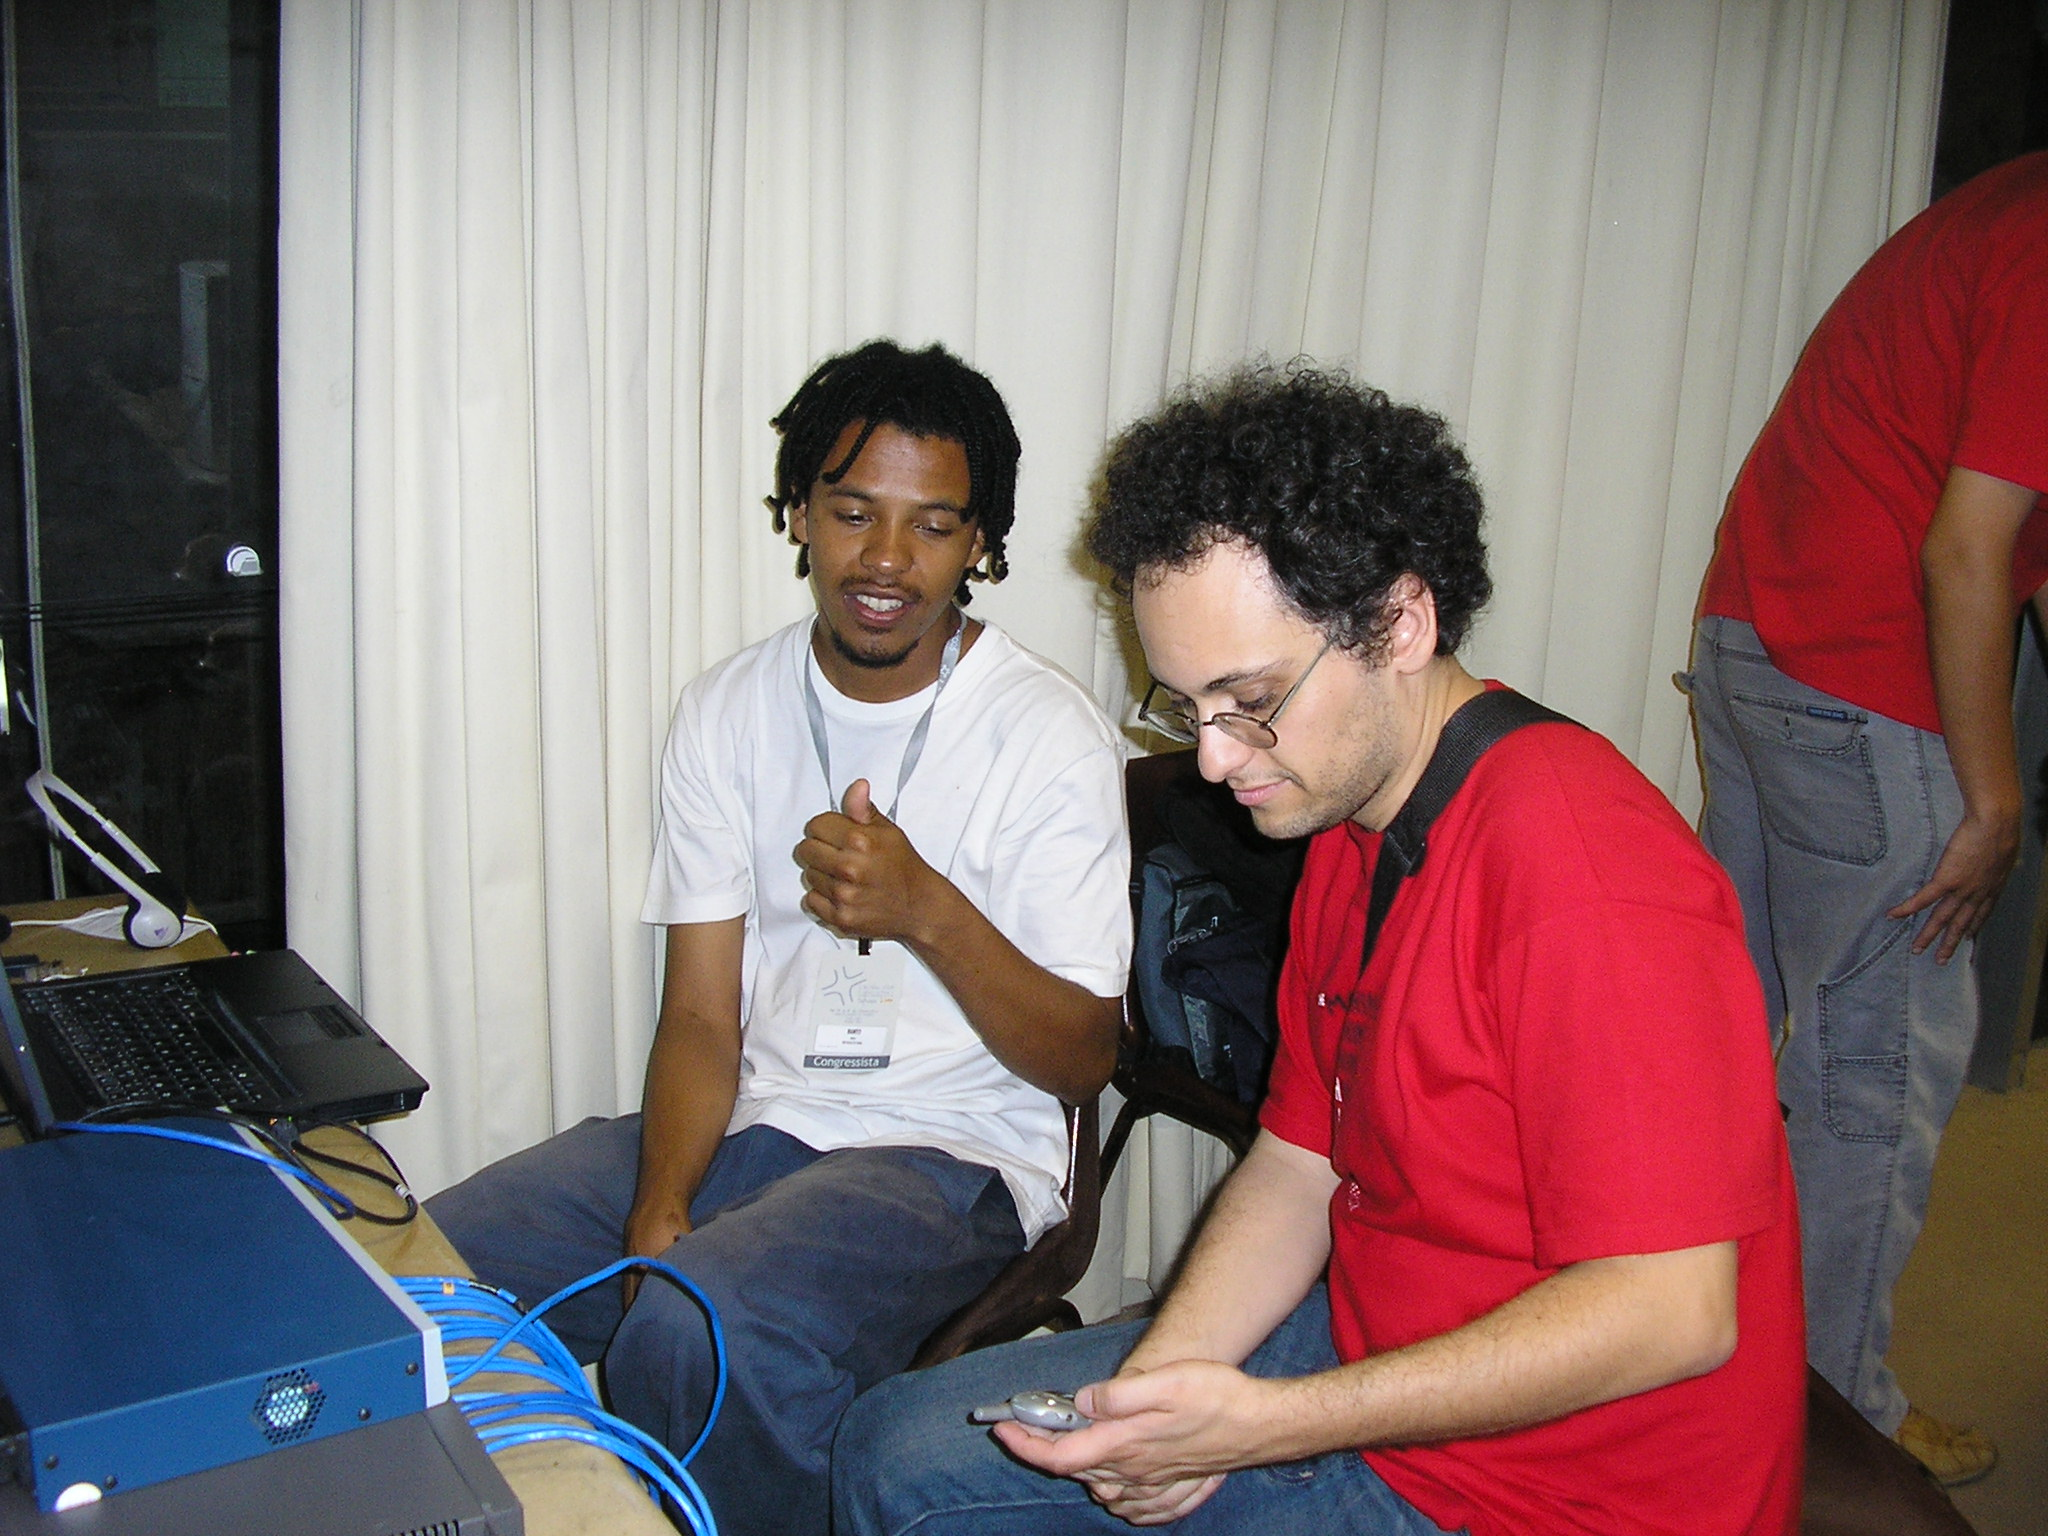
\includegraphics[width=1.0\linewidth]{../../../imagens/bantorafa.JPG}
                \caption{Oficina de formação de implementadores(as). Na foto vê-se Rafael Gomes da Cruz (i.e. Banto Palmarino). Banto foi posteriormente integrado à equipe do WASH, trazendo para o novo programa a experiência de multiplicação do GESAC.}
                \label{d2d74ac61c1b95a746858e8420d24348e1b48f51}
\end{minipage}%
\hspace{0.5cm}
\begin{minipage}[b]{0.4\linewidth}
        \centering
                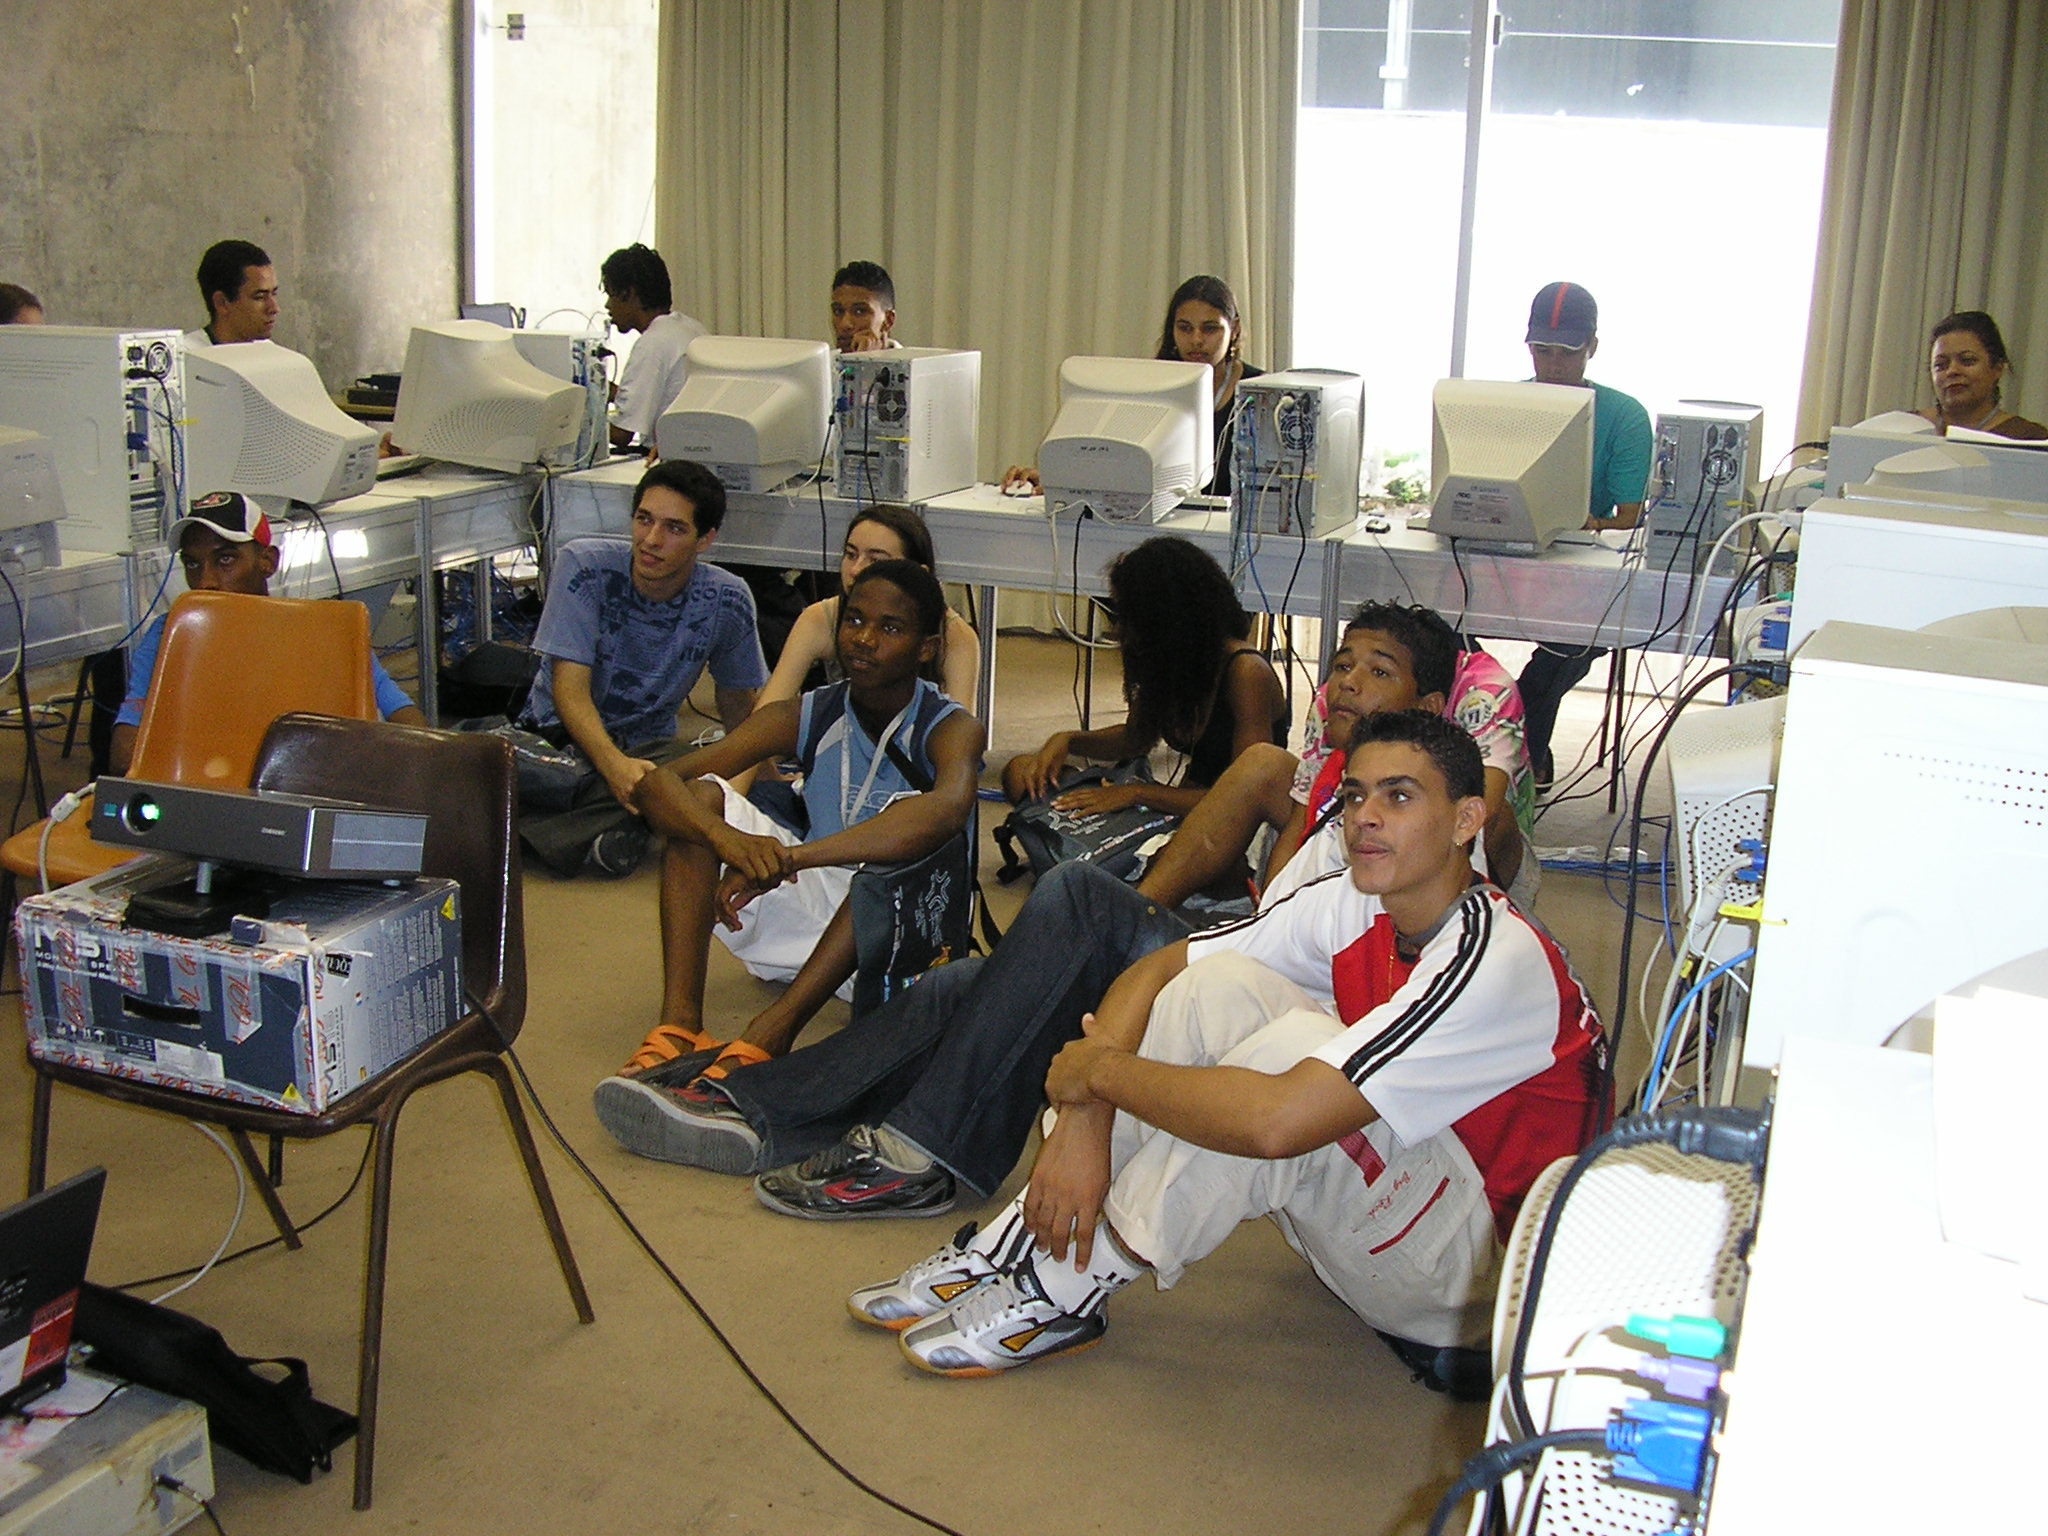
\includegraphics[width=1.0\linewidth]{../../../imagens/oficinalac.JPG}
                \caption{Oficina LacFree do GESAC, baseada sempre em conhecimentos livres.}
                \label{350ae75fda8eb19905317e70b64079af869125d8}
\end{minipage}
\hspace{0.5cm}
\begin{minipage}[b]{0.4\linewidth}
        \centering
                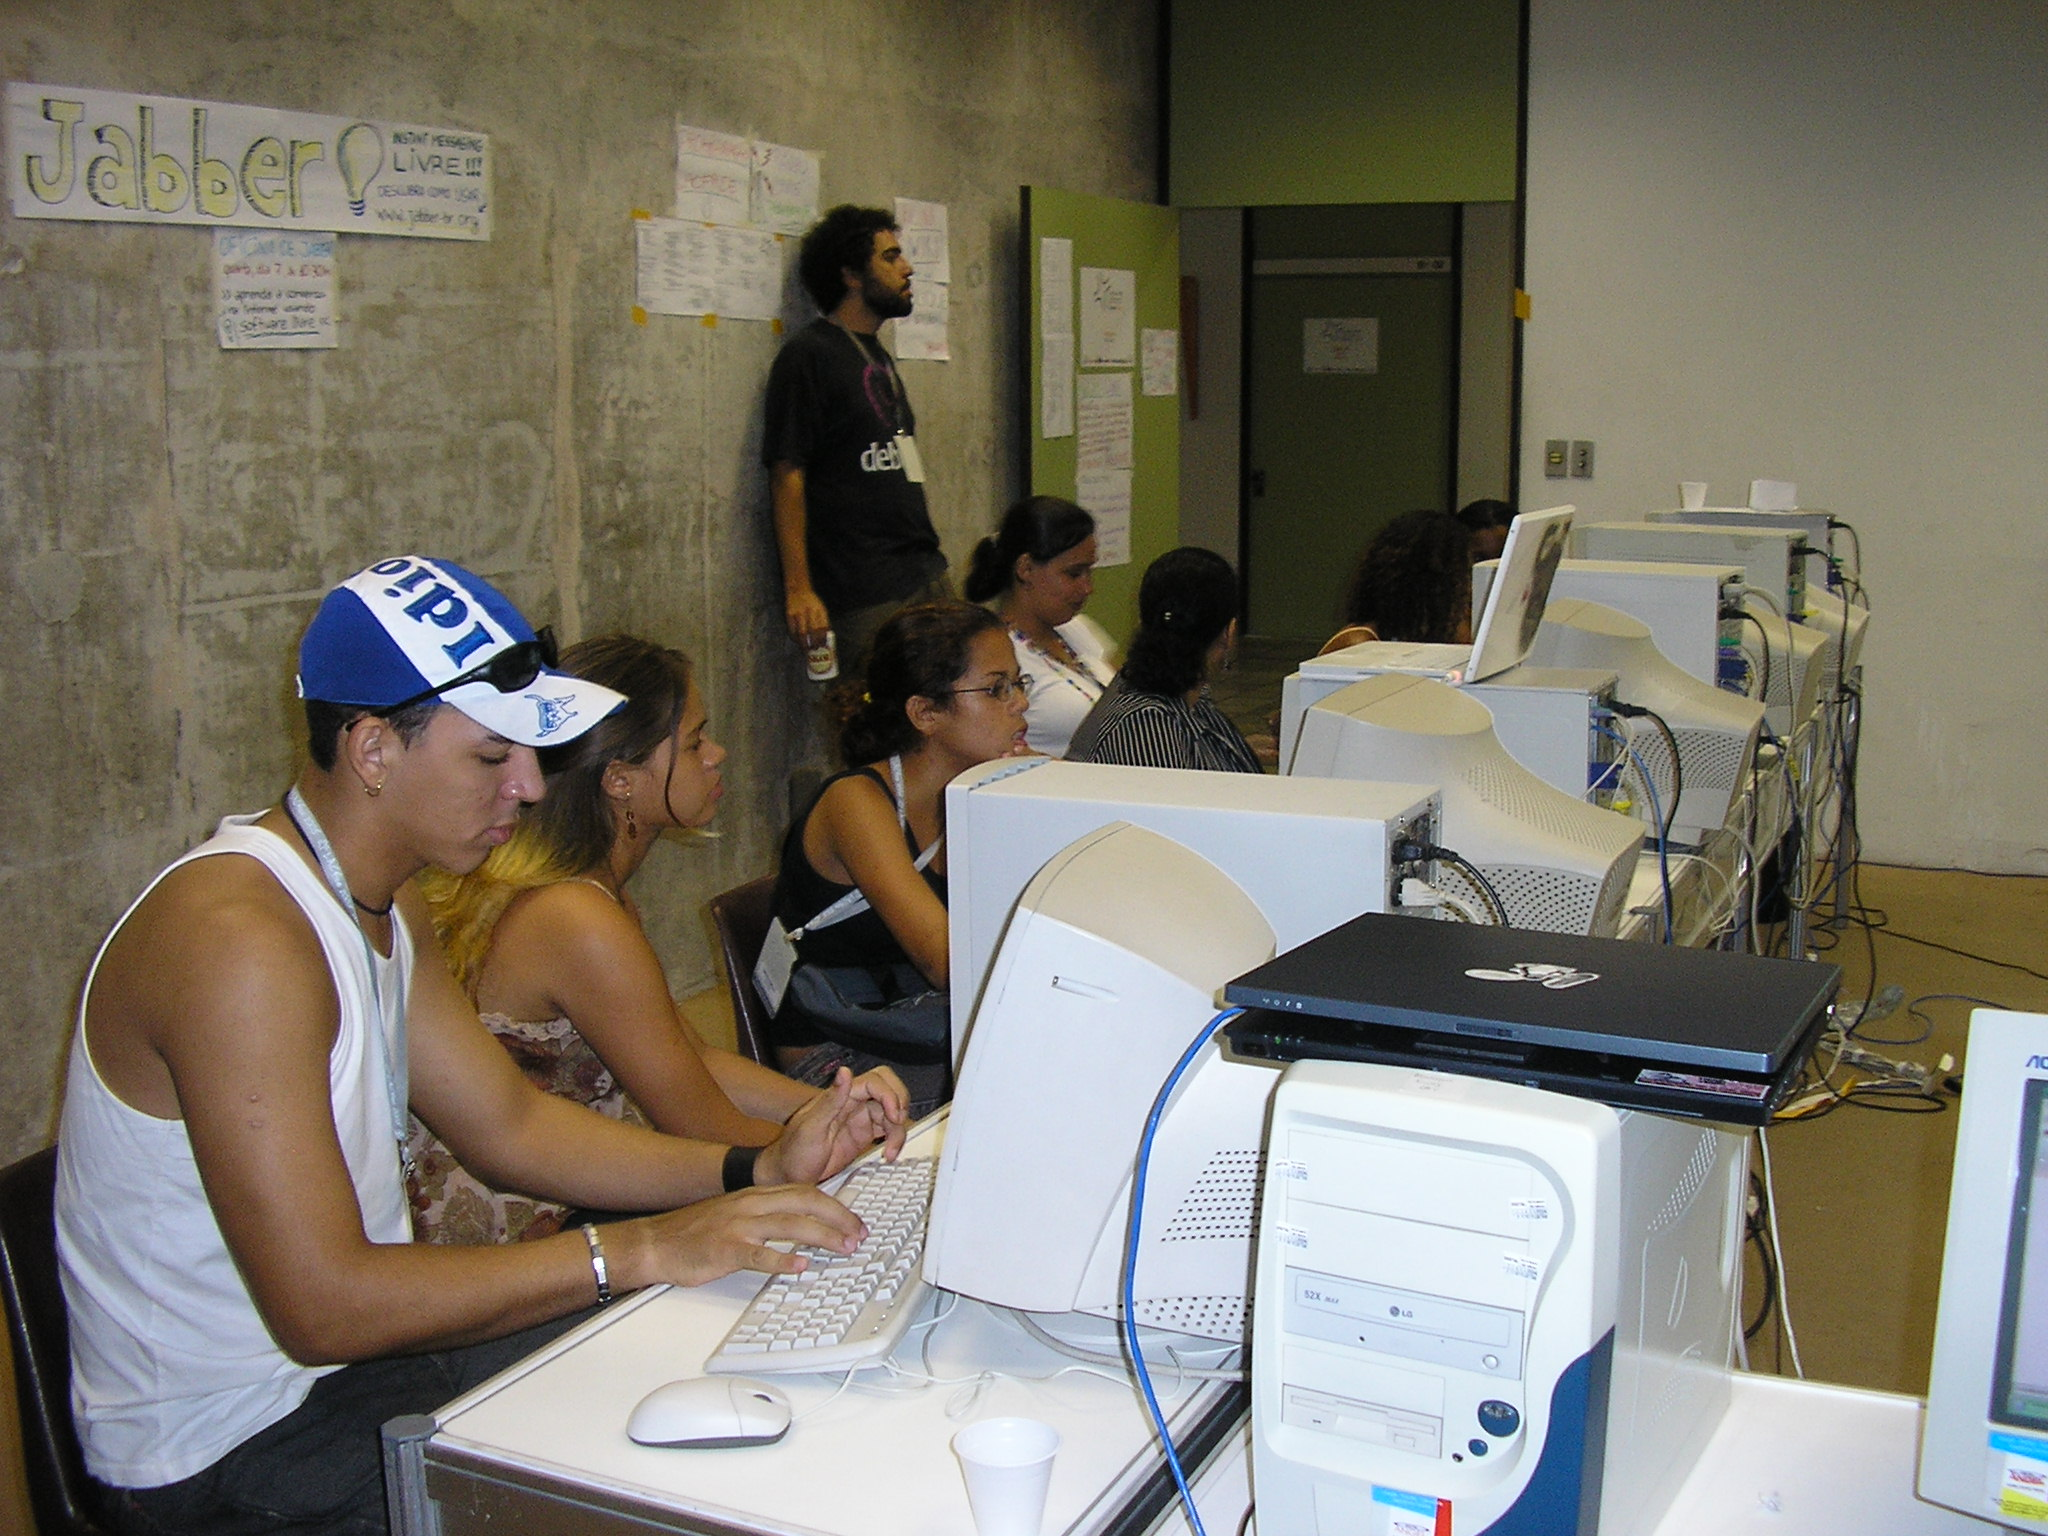
\includegraphics[width=1.0\linewidth]{../../../imagens/jabber.JPG}
                \caption{Oficina de Jabber com gestores.}
                \label{e29d9c3f5a4aa82fa420bc60ed161880a24bc2b6}
\end{minipage}%
\hspace{0.5cm}
\begin{minipage}[b]{0.4\linewidth}
        \centering
                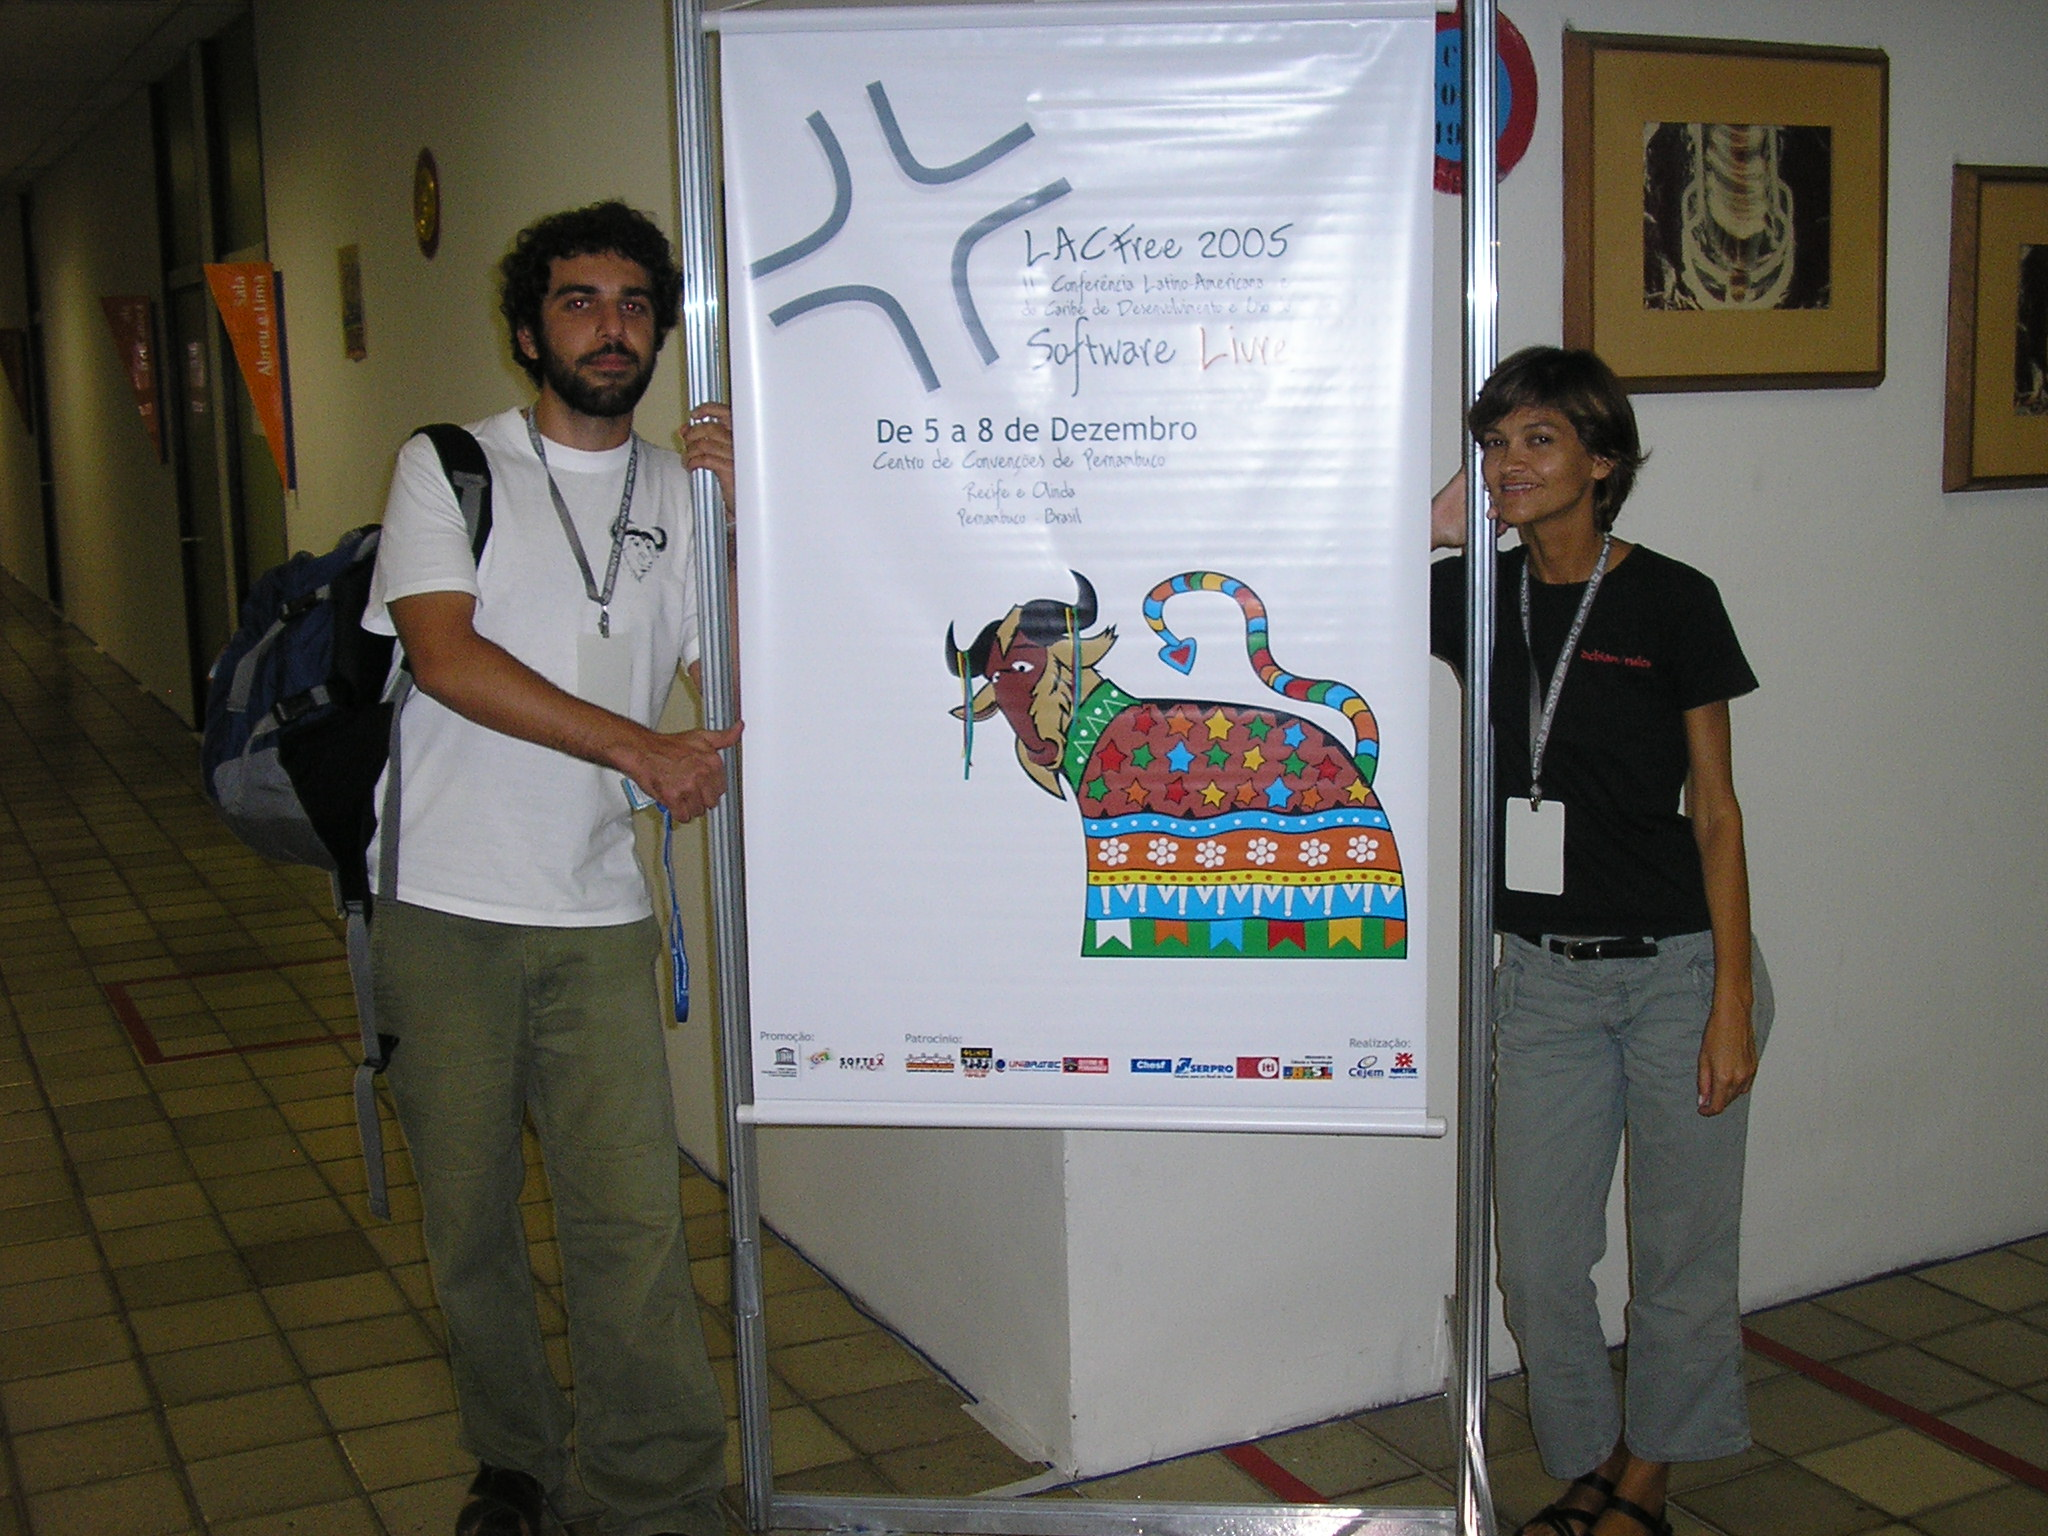
\includegraphics[width=1.0\linewidth]{../../../imagens/lacelavince.JPG}
                \caption{A presente autora, ao lado de Vincenzo Tozzi, implementador que também veio a contribuir com o WASH.}
                \label{4459669909728990ef00df4bdb6a369f3449704e}
\end{minipage}
\hspace{0.5cm}
\begin{minipage}[b]{0.4\linewidth}
        \centering
                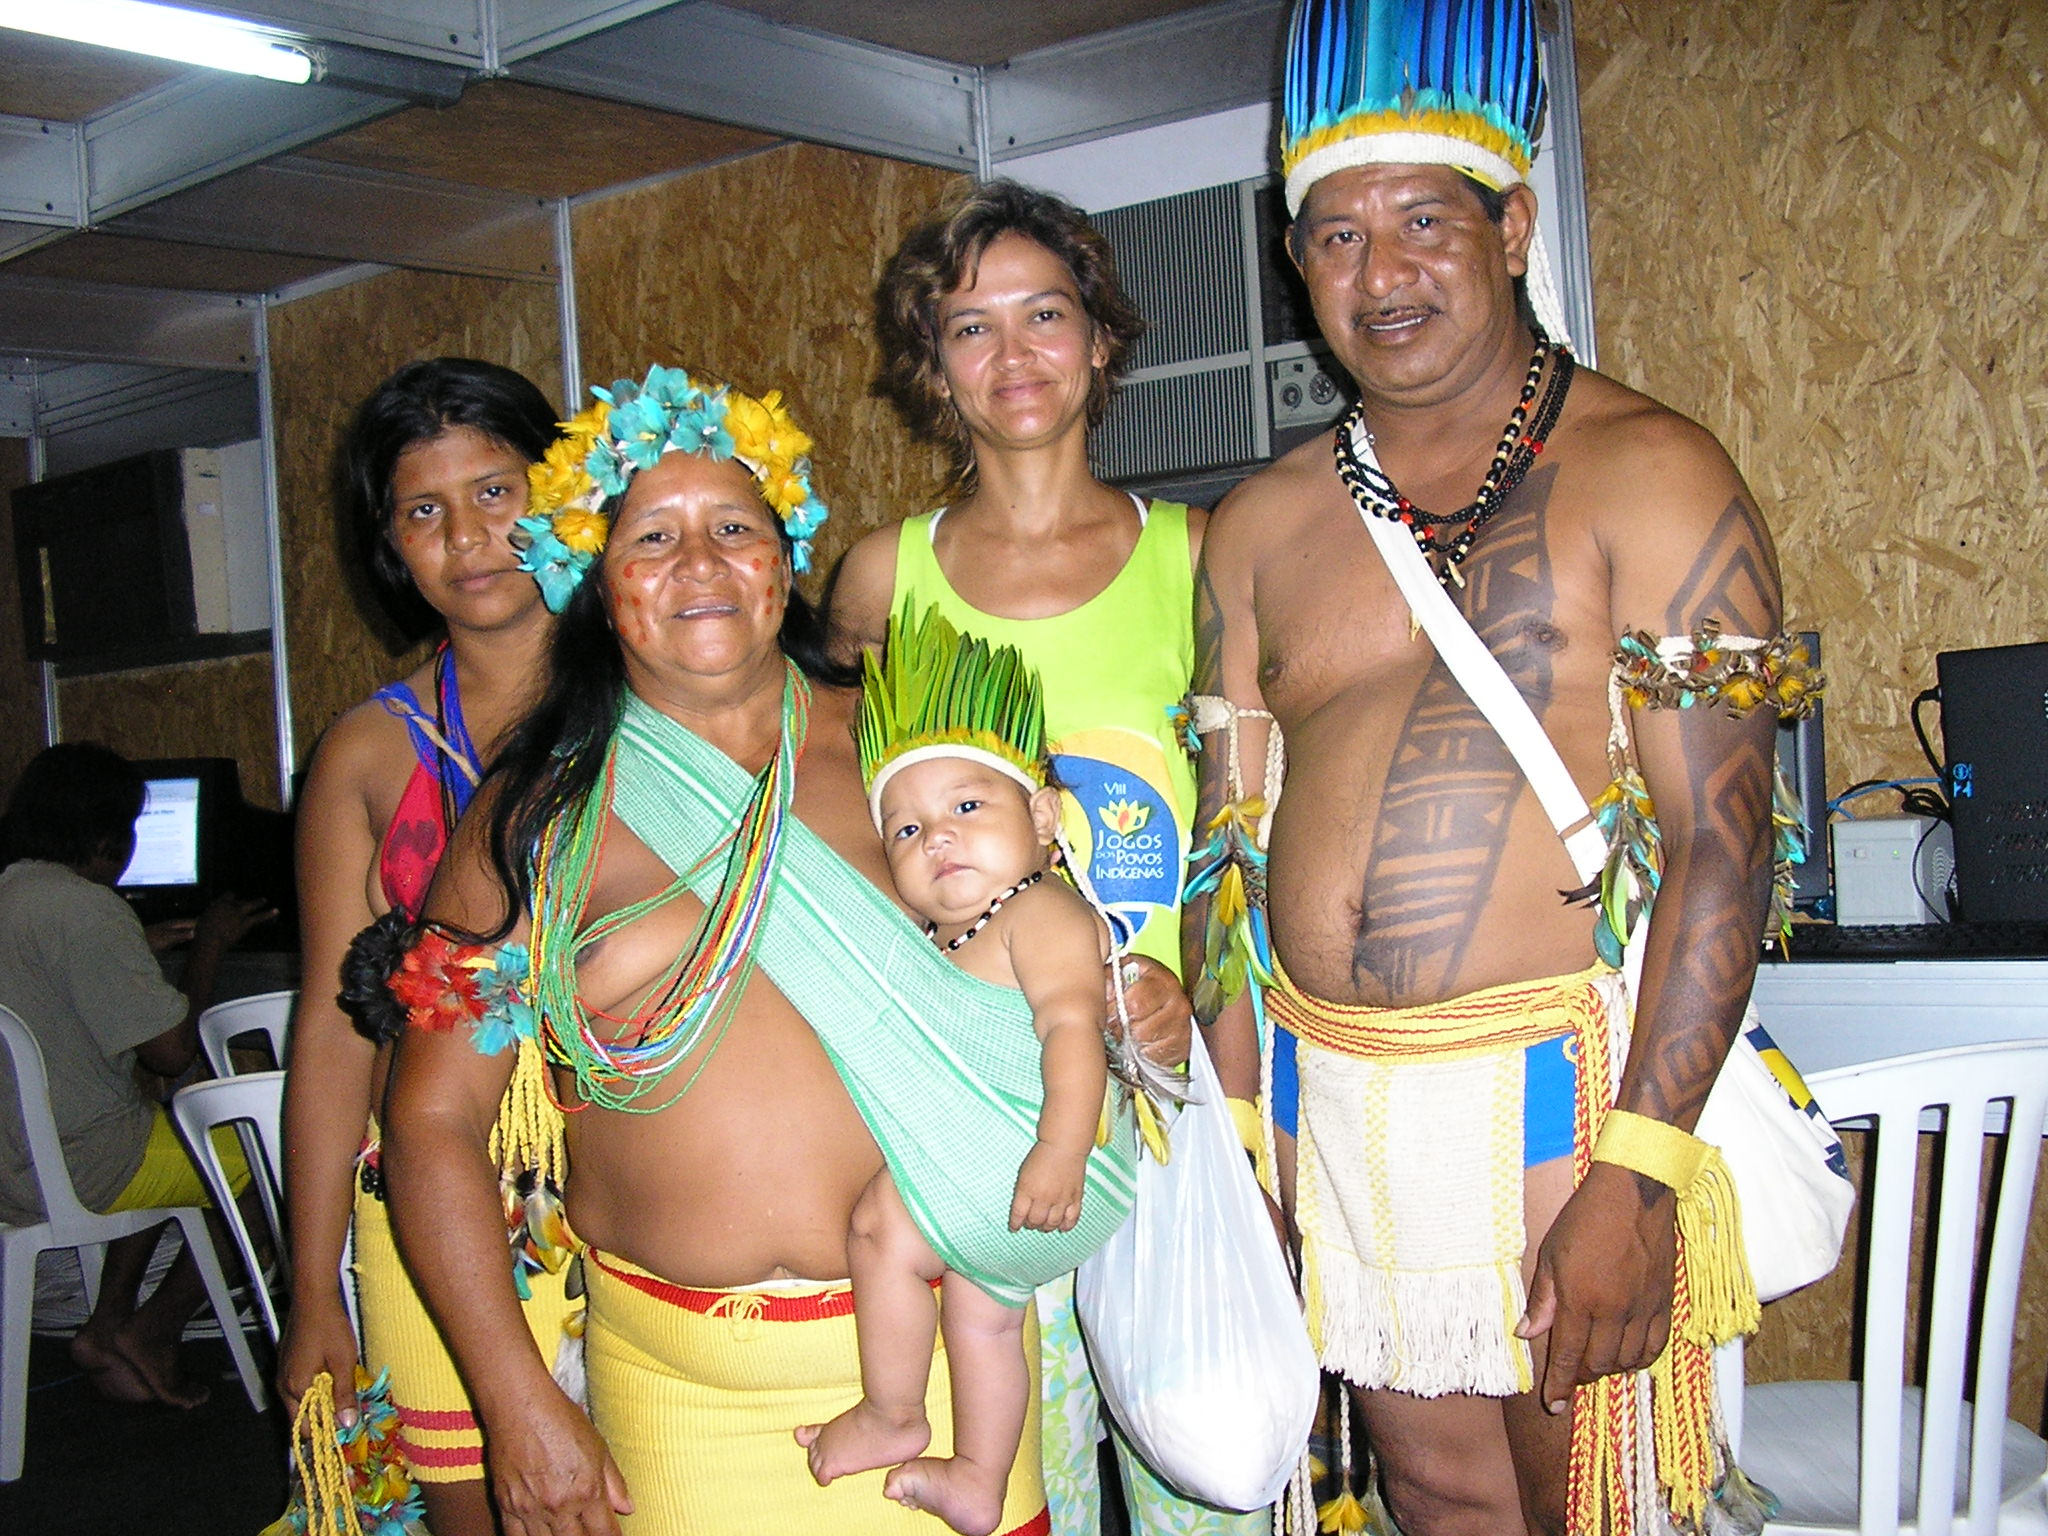
\includegraphics[width=1.0\linewidth]{../../../imagens/povo.JPG}
                \caption{Oficinas com indígenas eram muito comuns no GESAC.}
                \label{50c13a4f82feece9e41db915d8e5bc4c5d5094dd}
\end{minipage}%
\hspace{0.5cm}
\end{figure}



\subsection[A avaliação do OLPC pelo CTI como gênese do WASH]{A avaliação do OLPC pelo CTI como gênese do WASH}\label{A avaliação do OLPC pelo CTI como gênese do WASH}
Nesta seção fazemos uma interpretação sobre a gênese do Programa WASH, a partir do acervo de documentos por nós levantado. Foram utilizados, principalmente  os documentos referentes a duas avaliações conduzidas pelo coordenador do Programa WASH, na primeira década deste século:


\begin{itemize}
\item Avaliação do Projeto "One Laptop per Child" (OLPC) e sua versão brasileira, "Projeto Um Computador por Aluno" (UCA) (MAMMANA, 2006)
\item Avaliação do Programa de Inclusão Digital (PID) da Secretaria de Inclusão Social do Ministério da Ciência e Tecnologia (CGEE, 2010)
\end{itemize}

Além dos documentos citados, a presente seção se baseou em entrevistas com o Dr. Victor Pellegrini Mammana.

O Projeto "One Laptop Per Child" (NEGROPONTE, 2004) foi uma das iniciativas mais completas e robustas no sentido de ampliar a escala de aplicação das ideias de Papert. Ao mesmo tempo, era bastante polêmica, (ALVAREZ, 2015) por suas características disruptivas, alcance e ambição de crescimento, simultaneamente a uma certa desestruturação que prejudicava a confiança dos gestores públicos em sua viabilidade (MAMMANA e TOZZI, 2018).

Embora o Projeto OLPC estivesse no âmbito de uma Organização não Governamental independente,  foi concebido por pesquisadores do Massachusetts Institute of Technology (MIT), apoiados nas ideias e experiências de Seymour Papert (ALVAREZ, 2015). Especificamente, o Projeto OLPC é resultado das ideias debatidas por muitos anos no Media Lab, laboratório do MIT, do qual Papert foi Presidente do Conselho e Co-Fundador (ALVAREZ, 2015).

Os proponentes do OLPC tinham a ambição de que suas ideias fossem adotadas por países em desenvolvimento e, para isso, estabeleceram planos para regiões específicas do mundo, a exemplo do Brasil.

Em 2005, Nicholas Negroponte, idealizador do Projeto OLPC, apresentou sua ideia em Davos ([[MARKOFF, 2005]]). Naquela oportunidade, encontrou-se com representantes do Governo Brasileiro (ALVAREZ, 2015) que organizaram um encontro com o presidente Lula, o qual foi realizado em junho daquele ano (ALVAREZ, 2015) (CRISTINA, 2005).

Como resultado dessas tratativas iniciais, o documento intitulado "Brazil Plan " (NEGROPONTE, 2004), fonte primária para a construção da presente narrativa, foi direcionado à "Brazilian Task Force", tendo sido compartilhado com o governo brasileiro, em 2005.

O OLPC era explicitamente apoiado por Papert, quando ainda estava vivo, tendo contado com sua presença ativa e eloquente nas reuniões de apresentação do OLPC para o Governo Brasileiro, inclusive em uma visita ao presidente Lula (ver Fig. 21).



\captionsetup{format=plain}
\begin{figure}[p]

\centering


\begin{minipage}[b]{0.4\linewidth}
        \centering
                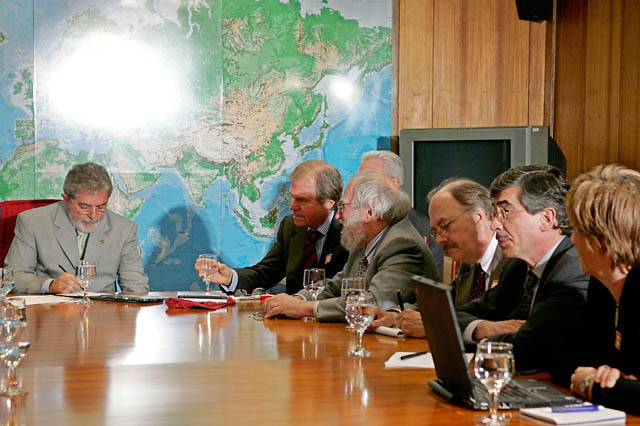
\includegraphics[width=1.0\linewidth]{../../../imagens/lula-papert.jpg}
                \caption{Presidente Lula, Negroponte, Papert, Rodrigo Mesquita e Mary Lou Kepsen (fonte: flicker de Rodrigo Mesquita).}
                \label{7c0febad22b3e599a6886b31cdcbd3be3ce60df2}
\end{minipage}%
\hspace{0.5cm}
\begin{minipage}[b]{0.4\linewidth}
        \centering
                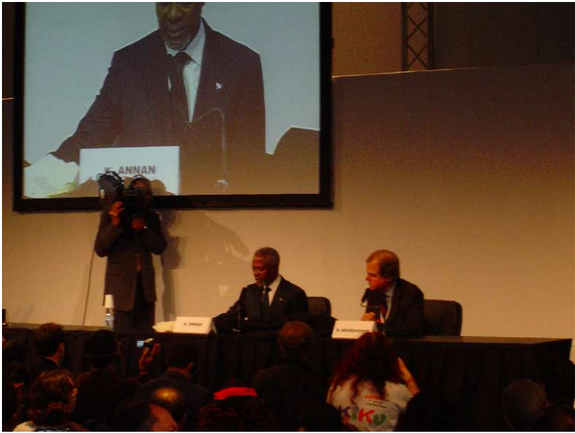
\includegraphics[width=1.0\linewidth]{../../../imagens/Kofi-negroponte.png}
                \caption{Nicholas Negroponte apresentando o protótipo do OLPC para o Secretário Geral da ONU, Kofi Anan (crédito: Victor Mammana, 2005).}
                \label{31f6206a8e4662597d5a134974d64a4696f4129c}
\end{minipage}
\hspace{0.5cm}
\begin{minipage}[b]{0.4\linewidth}
        \centering
                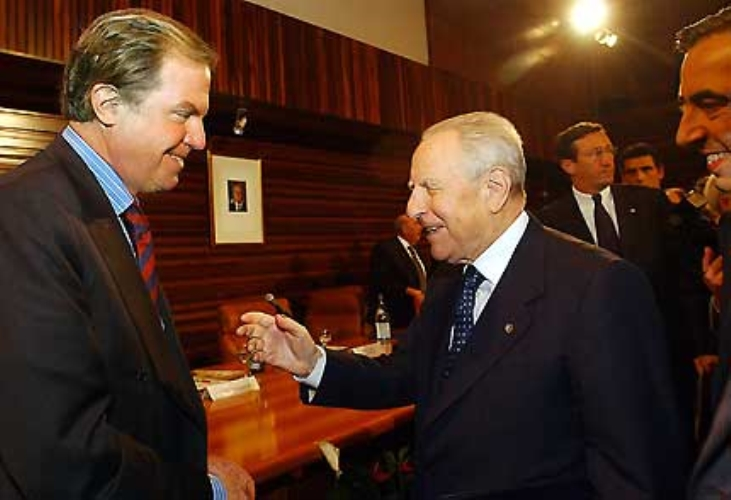
\includegraphics[width=1.0\linewidth]{../../../imagens/presidente-italia.jpg}
                \caption{Nicholas Negroponte com o presidente da Itália, em 2003.}
                \label{f15f5d2fa7b78d2e6dec6ac4a7be76d564c9bf71}
\end{minipage}%
\hspace{0.5cm}
\begin{minipage}[b]{0.4\linewidth}
        \centering
                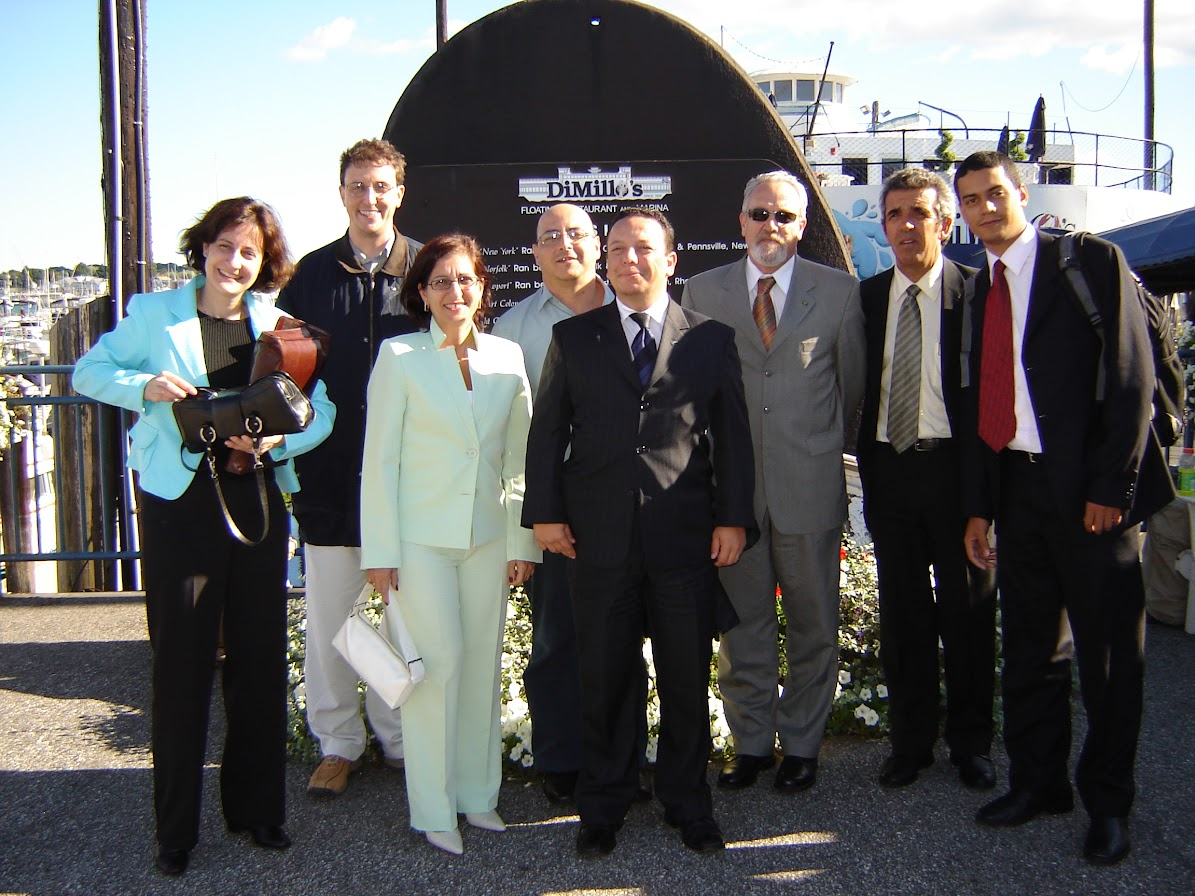
\includegraphics[width=1.0\linewidth]{../../../imagens/equipeOLPC.jpg}
                \caption{Missão Brasileira de avaliação da proposta OLPC, em visita ao Maine em 2005. (fonte: acervo pessoal)}
                \label{b1b538b3cf66c3aaf3d7a74aac4332a1f40be14d}
\end{minipage}
\hspace{0.5cm}
\end{figure}



Nicholas Negroponte, o líder da iniciativa do OLPC, era um destacado "guru " tecnológico, professor do MIT, cofundador da revista Wired e tinha acesso a chefes de estado, a exemplo do presidente Miterrand, da França que, na década de 80, foi apoiador da criação do "Centre mondial informatique et ressource humaine", onde Negroponte atuou como dirigente. Coincidentemente, era irmão de John Negroponte, então Secretário de Estado do Governo Bush, diplomata americano influente nos meios políticos, na comunidade de informação e em outras áreas estratégicas e de defesa daquele país.

A referência ao "Centre mondial informatique et ressource humaine" assume uma particular importância nesta narrativa, uma vez que um outro partícipe desta história, o Prof. Jose Ellis Ripper Filho (esposo da Profa. Afira Ripper) foi membro do conselho dessa instituição francesa, estabelecendo um emaranhado de relações entre seus atores, ao longo de várias décadas. No período em que atuou como conselheiro, a convite de Miterrand, o Prof. Ripper chegou a interagir diretamente com Negroponte, muito antes da concepção do OLPC.

Nicholas transitava com razoável desenvoltura entre líderes mundiais, a exemplo de Kofi Anan (ver Fig. 22), Lula (ver Fig. 21), Mitterrand ou o presidente da Itália (ver Fig. 23). Essa presença junto a governos criou a oportunidade para que, em 2006, países como Argentina, Nigéria, China, Índia, Egito e Costa Rica participassem das tratativas do OLPC  (pág. 84 de (ALVAREZ, 2015).

A proposta era ousada e atraente no que tange à transformação dos métodos pedagógicos. Por outro lado, era também exigente em termos de recursos, uma vez que preconizava a aquisição de milhões de notebooks como forma de empoderamento dos estudantes pela possibilidade de conexão à internet  (NEGROPONTE, 2004). Em termos orçamentários, a adesão à proposta de Negroponte representava um valor significativo do orçamento do Ministério da Educação (cerca de quatro bilhões de dólares) e havia o entendimento do governo brasileiro de que, para que fosse viabilizado no país, o OLPC precisaria passar por um escrutínio da sociedade brasileira.

Ciente do risco que representava uma adesão voluntariosa a um programa tão disruptivo, a Presidência da República da época decidiu estabelecer um grupo de avaliação  daquela proposta, o  qual foi constituído por universidades e centros de pesquisa. Foram chamados o Centro de Tecnologia da Informação Renato Archer (CTI), a Escola Politécnica da USP e a Fundação CERTI (ALVAREZ, 2015). A Fig. 24 traz uma imagem de uma parte da missão brasileira, constituída para avaliar o OLPC, em visita ao Maine em 2005.

Coordenavam as atividades de avaliação, o assessor especial da Presidência da República, Dr. César Santos Alvarez, e o secretário de Política de Informática, Dr. Marcelo Lopes.

O grupo de três entidades de pesquisa tinha como intuito:


\noindent\begin{center}\mbox{\centering\fbox{\centering\par\parbox{0.7\linewidth}{\small\textit{"verificar sua adequação (OLPC) à realidade nacional dentro das expectativas do governo de investir em processos de melhoria da qualidade da educação brasileira"  (MEC, 2006 apud ALVAREZ, 2015)}\normalsize}}}\end{center}


As instituições mencionadas avaliaram o projeto em vários aspectos  (MAMMANA, 2005):


\begin{itemize}
\item proposta pedagógica;
\item modelo de negócios;
\item cadeia de fornecimento;
\item sistema de qualidade;
\item produção;
\item software;
\item ergonomia;
\item certificação e normas técnicas;
\item displays;
\item mock-ups;
\item usabilidade;
\item arquitetura de referência;
\item avaliação experimental; e
\item rede.
\end{itemize}

A proposta previa a aquisição de um "laptop" por estudante brasileiro, ou seja, perto de 30 a 40 milhões de unidades.

Segundo a visão trazida pelo OLPC  (NEGROPONTE, 2004) ao governo brasileiro, a disponibilização em larga escala de acesso à internet alteraria a relação aluno-professor, promovendo formas de aprendizagem alternativas ao conteudismo tradicional, reformulando também o formato lousa-giz inerente ao sistema educacional brasileiro.

Um dos aspectos principais do projeto apresentado ao governo, do ponto de vista de software, era a disponibilização de uma ferramenta de programação mais intuitiva e lúdica do que o próprio LOGO, linguagem criada por Papert e colegas na década de 60 e que se disseminou por todo o mundo (ver Fundamentação Teórica).

Das três instituições envolvidas na avaliação do OLPC, tivemos acesso à avaliação do CTI  (MAMMANA e TOZZI, 2018), que ficou encarregado da:


\begin{itemize}
\item avaliação de características de ergonomia postural, por meio da captura de movimento;
\item avaliação de características de ergonomia sensorial, por meio de técnicas relacionadas à área de mostradores de informação;
\item avaliação da funcionalidade dos "laptops", principalmente em termos de redes, processamento, memória e baterias;
\item avaliação do emprego dos dispositivos  da escola pública;
\item avaliação da percepção dos professores sobre o projeto;
\item análise da infraestrutura das escolas, visando verificar a viabilidade de implantação do projeto;
\item acompanhamento de pilotos de avaliação em escolas públicas brasileiras; e
\item visitas a pilotos nos Estados Unidos.
\end{itemize}

Do ponto de vista da aquisição de "laptops " em larga escala, o CTI identificou uma série de dificuldades nas seguintes áreas: apropriação pela escola brasileira, produção dos laptops, restrições orçamentárias, falta de visão clara sobre o controle dos conteúdos, falta de uma visão sobre capacitação dos profissionais da educação, problemas ergonômicos e, principalmente, obsolescência dos equipamentos (MAMMANA e TOZZI, 2018). Estes aspectos demonstraram que a ideia de aquisição de milhões de laptops representava um risco muito grande para o sistema educacional brasileiro.

O estudo apontava, também, que o sistema educacional poderia se beneficiar de alguns aspectos da proposta, mas que qualquer iniciativa disruptiva no sistema educacional brasileiro requereria mais investimentos em capacitação de recursos humanos do que em hardware ou software, ao contrário do que propunha o Projeto OLPC, que focalizava a aquisição dos computadores.

A percepção de que o Projeto OLPC, como proposto por Negroponte, tinha um equívoco em seu foco foi expressa principalmente pela equipe do CTI, que se destacou dos demais participantes da avaliação, que estavam mais propensos a apoiar o projeto como originalmente proposto. A posição do CTI se sustentava na própria definição de educação empregada na análise da proposta OLPC: "Educação é a inserção do indivíduo em sua própria cultura, através da interação com outros indivíduos".

Esta definição colocava a interação entre indivíduos no centro do processo e, portanto, qualquer esforço de qualificação da escola brasileira precisaria passar por uma ênfase no investimento em "pessoas, mais do que em software ou hardware ".

A proposta do MIT envolvia abordagens pedagógicas que buscavam combinar elementos de um amplo espectro de correntes distintas, que partiam de Piaget, passando por Vygotsky, Dewey e chegando em Paulo Freire  (NEGROPONTE, 2004).

Não obstante essa pluralidade conceitual, o documento do OLPC não escondia a prevalência do pensamento de Papert (que na época ainda era vivo) na concepção da proposta apresentada ao Governo Brasileiro.


\noindent\begin{center}\mbox{\centering\fbox{\centering\par\parbox{0.7\linewidth}{\small\textit{(...) um dos aspectos mais atraentes da proposta é a ênfase em “estratégias para aprender o que não se sabe” ao invés de focalizar “em ensinar o que os outros devem saber”. Esta mudança de foco no processo educacional, segundo os argumentos apresentados, seria possível através do emprego de dispositivos digitais portáteis conectados à internet, que devem superar os problemas oriundos de técnicas tradicionais de ensino. O programa, segundo o MIT, oferece uma solução para os problemas que “foram formulados (mas, talvez, nunca resolvidos) por Jean Piaget, Paulo Freire, John Dewey e Lev Vygotsky”. (Fonte: tradução livre de (NEGROPONTE, 2004)}\normalsize}}}\end{center}


Um outro aspecto do programa era o foco na "propriedade de um bem de informática em detrimento do compartilhamento destes recursos em um laboratório de computadores". A visão da época considerava que a doação de um laptop com acesso irrestrito à internet deveria ser a base de um novo processo educacional (MAMMANA, 2006). Este enfoque buscava enfrentar uma deficiência de programas anteriores como o PROINFO do MEC, que por ser desprovido de uma visão pedagógica estruturada sobre o uso de computadores, deixando o controle de acesso aos laboratórios para profissionais sem uma capacitação específica, resultou em uma profusão de relatos de "laboratórios de micros trancados" (ver Fig. 25)  (CNPq, 2020). No OLPC não existiria restrição de acesso aos computadores, porque os donos dos equipamentos eram os próprios estudantes. Mas, esta "vantagem" não trazia luz sobre  uma questão que surgiria imediatamente após a doação do laptop para a criança: vão fazer o que com isso?



\captionsetup{format=plain}
\begin{figure}[htb]

	\begin{center}

		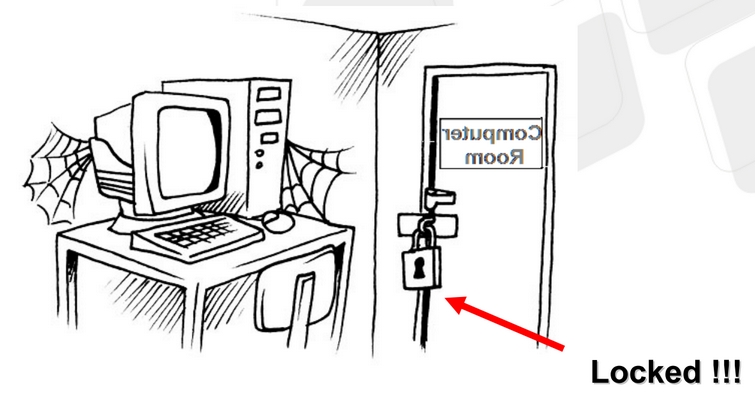
\includegraphics[max size={\textwidth}{\textheight}]{../../../imagens/computer-room.png}

	\end{center}

	\caption{\label{5817b264c8a300b4b46214039b2e579aba5d70a7}Arte produzida sob encomenda para a avaliação do OLPC, expondo a situação dos laboratórios de micro-computadores de muitas escolas brasileiras no final de século XX, início do XXI. (Fonte: acervo pessoal de Victor Mammana)}

\end{figure}

A avaliação do Governo Brasileiro já percebia que o OLPC exagerava o papel que uma simples ferramenta digital (laptop) poderia desempenhar no processo educacional, mas reconhecia que o uso desta ferramenta na escola poderia "permitir uma melhor preparação para a sobrevivência do educando na sociedade de informação, criando oportunidades para sua inclusão como membro ativo desta sociedade".

Mas, o projeto também criava muita insegurança nas autoridades brasileiras e, a partir de agora, citamos algumas com base nos achados descritos por (MAMMANA, 2006) em seu relatório final de avaliação, concentrando-nos em questões de cunho estratégico e geopolítico:


\begin{itemize}
\item "Em última análise, o OLPC é um projeto de poder, com méritos e agendas alternativas às dos Estados Nacionais, que atua na área mais sensível de qualquer sociedade: sua reprodução e reinvenção, ou seja, a educação;"
\item "A adesão ao OLPC coloca a internet no centro do processo de aprendizagem, promovendo a convergência final entre educação e mídia; "
\item "A despeito de qualquer paranóia, a previsão de qual é a direção e evolução do controle da internet é objeto de muita controvérsia em todos os meios, mas deve ser tema de reflexão por parte das autoridades que decidirão pela adesão ao OLPC, pela relevância que a mesma assume no contexto do programa;"
\item "O que deve ser evitado pelo governo brasileiro é a adesão extemporânea a um projeto cuja a agenda é controlada por grupos que não estão sob a esfera de influência do poder democrático, instituído em nosso país;"
\item "Mais do que a convergência de tecnologias de informação e comunicação (TICs), a proposta OLPC traz, em si, a convergência da mídia com a educação, quando esta última passa a ser, definitivamente (e pela ausência de uma visão de cidadania associada), dominada por agentes econômicos globais que custodiam e controlam os conteúdos que até agora têm sido oferecidos democraticamente pela sociedade aos seus repositórios;"
\item "Através de uma intensa atividade de persuasão nas estruturas de poder de vários países, os representantes da Organização OLPC, que em parte são oriundos do Media Lab, vêm buscando a adesão de diversos governos do mundo para um programa de adoção de laptops de baixo custo nas atividades curriculares de suas redes de ensinos fundamental e médio. Simultaneamente, a esta atividade com os governos, é razoável acreditar que a Organização OLPC está, também, estabelecendo contratos e acordos que não têm sido divulgados ao público e a estes governos. Uma das justificativas para essa não divulgação pode ser a preocupação com forças antagônicas da indústria, as quais, por terem seu mercado ameaçado, podem se utilizar destas informações estratégicas para reagir à implementação do OLPC;"
\item "A proposta OLPC é parcialmente financiada por agentes, que a imprensa frequentemente associa ao universo de think tanks conservadores e ONGs com interesse geopolítico [1], além de empresas de Mídia com possível interesse no acesso a novos mercados, como é o caso da Google; e
\item "Subjacente a visão do OLPC está a viabilização do acesso irrestrito a informações que, se por um lado hoje têm diversidade impressionante e acredita-se, estão disponíveis de forma democrática na internet; por outro lado estão sob custódia e escrutínio de estruturas de disseminação de informação dominadas por empresas privadas globais, num modelo de governança da internet que atribui a um único Estado hegemônico o poder discricionário sobre toda a rede (ICANN)."
\end{itemize}

Os pontos levantados pela avaliação do OLPC por, parte de pesquisadores brasileiros,levaram a um alerta, seguido de uma recomendação:


\noindent\begin{center}\mbox{\centering\fbox{\centering\par\parbox{0.7\linewidth}{\small\textit{"(...) Neste contexto, deve ser evitada a adesão extemporânea a um projeto cuja a agenda é controlada por grupos que não estão sob a esfera de influência do poder democrático, instituído em nosso país. (...) A impossibilidade de prever o que pode acontecer e a certeza de que existem consequências para o modelo de democracia brasileiro devem ser o pano de fundo para a tomada de decisão sobre o que fazer com o OLPC. Embora nenhuma ação nesta direção tenha sido tomada, sabe-se que há como enquadrar o OLPC naquilo que a sociedade considerar mais conveniente para a cidadania do brasileiro." (Fonte: MAMMANA, 2006)}\normalsize}}}\end{center}


Percebe-se, no posicionamento acima, uma preocupação com a possibilidade de formação de estruturas de disseminação de informação em que os valores da cidadania poderiam deixar de ser preponderantes. Em parte, pode-se dizer que as redes sociais de hoje estão se prestando a esse serviço, transformando-se em meios para a disseminação de informações falsas, ideologias de ódio, crimes, entre outros. Interpretando, a posteriori, e por meio de comunicação privada recente do autor de uma das avaliações, parece-nos que o posicionamento do CTI se insurgia contra a subordinação da escola brasileira, berço de nossa cidadania, a esse poder monumental. Talvez o CTI tenha "farejado" e antecipado algo que veio a ser testemunhado nos dias de hoje, quando as redes sociais, fora do contexto da escola, se transformaram efetivamente num instrumento de disseminação de informações falsas, teorias da conspiração, entre outras formas de criação de realidades paralelas.

Dentre as atividades atribuídas a Victor Mammana, no período de avaliação do OLPC, estava o acompanhamento do desenvolvimento do laptop em si, aproveitando a experiência do mesmo com política industrial na área de mostradores de informações (displays). Essa atividade contribuiu para avaliar a viabilidade tecnológica das soluções propostas.

A Fig. 26 mostra uma foto emblemática da situação do desenvolvimento do OLPC, no momento em que o fornecimento dos laptops para o Brasil era negociado, que gerava muita insegurança no Governo Brasileiro. Na foto, tirada por Victor Mammana, é possível ver que o "protótipo" apresentado a Kofi Anan não tinha "placa mãe" e não era um produto real. A eletrônica que "dava vida" ao mock-up do laptop estava embaixo da mesa. Um extenso relatório foi apresentado ao coordenador da Força Tarefa Brasileira de avaliação do OLPC, Dr. César Alvarez, gerando questionamentos à equipe do OLPC sobre o real estágio de desenvolvimento do protótipo do dito "laptop de 100 dólares, " naquele crucial momento. (MAMMANA, 2005).



\captionsetup{format=plain}
\begin{figure}[htb]

	\begin{center}

		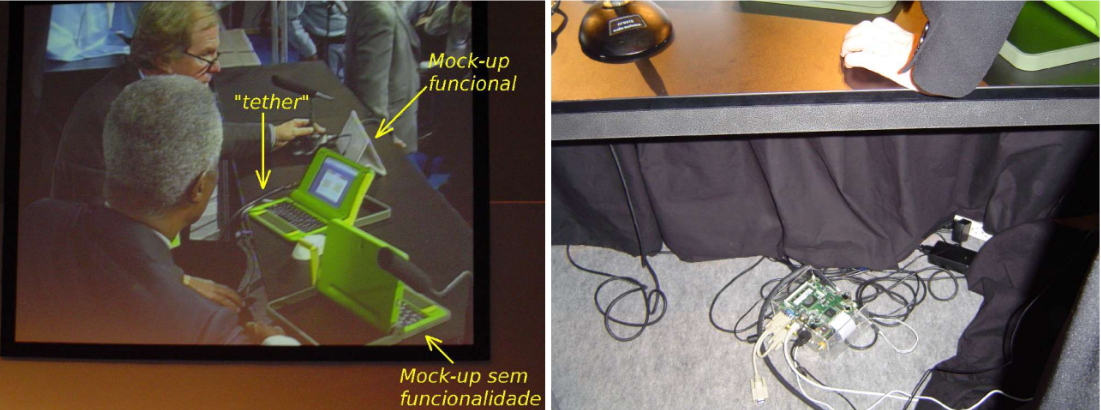
\includegraphics[max size={\textwidth}{\textheight}]{../../../imagens/embaixo-mesa.png}

	\end{center}

	\caption{\label{009ca00e74581d7c5448a43112358cb91a959b69}Foto tirada por Victor Mammana mostrando que o OLPC ainda não tinha um protótipo completo, mesmo com as negociações avançadas com o Governo Brasileiro. Essa situação gerou muita insegurança na Presidência da República. (créditos: Victor Mammana)}

\end{figure}

Sobre essa situação, (MAMMANA, 2006) alertava:


\noindent\begin{center}\mbox{\centering\fbox{\centering\par\parbox{0.7\linewidth}{\small\textit{"Do ponto de vista técnico, é preciso estar atento às críticas referentes à maneira desestruturada com que vêm sendo proposto, gerando preocupações sobre sua viabilidade pedagógica, industrial, financeira e social, no longo prazo." (Fonte: (MAMMANA ,2006)}\normalsize}}}\end{center}


Outro aspecto analisado foi a ergonomia, tendo sido constatado que laptops são intrinsecamente não ergonômicos, por justapor tela e teclado numa mesma "caixa". Essa constatação pode ser sumarizada nesta frase: "quando a tela está numa posição adequada para os olhos, o teclado fica em posição inadequada, e vice-versa"(HIRAGA et al., 2006).

Sobre isso, (HIRAGA et al. (2006) constatava:


\noindent\begin{center}\mbox{\centering\fbox{\centering\par\parbox{0.7\linewidth}{\small\textit{"Ficou evidente que o projeto OLPC não leva em conta aspectos importantes de ergonomia quanto ao uso saudável do laptop como, por exemplo, a postura corporal do usuário, o tempo de uso, o mobiliário a ser utilizado, entre outros." (Fonte: HIRAGA et al, 2006)}\normalsize}}}\end{center}


Ao longo das análises presentes nas dezenas de relatórios de avaliação gerados, muitas outras questões criaram questionamentos cujas respostas não pareciam satisfatórias, a exemplo de:


\begin{itemize}
\item obsolescência dos equipamentos e descarte seguro de lixo-eletrônico;
\item custo de aquisição para o governo brasileiro;
\item manutenção dos equipamentos;
\item garantia de acesso à internet no prazo necessário;
\item segurança das crianças em vários aspectos (e.g. conteúdos impróprios, exposição a situações de risco nas redes sociais);
\item capacitação dos profissionais de educação para promover a melhor utilização dos equipamentos; e
\item custo da infraestrutura periférica (adequação do mobiliário, sistemas de carregamento de baterias, entre outros).
\end{itemize}

Em suma, o que se constatou é que, pelas dimensões do Brasil e os prazos exíguos de adesão exigidos pelo OLPC, havia muitos riscos para o sistema educacional brasileiro. Por outro lado, para países menores, a adesão poderia fazer mais sentido, dado que essas questões poderiam ser tratadas com mais detalhe e controle.

Não obstante todas estas dúvidas, o valor da proposta OLPC foi reconhecido. É possível identificar na documentação existente a ânsia dos pesquisadores envolvidos em encontrar uma alternativa que fosse mais adequada à realidade brasileira, mas que, ao mesmo tempo, permanecesse usufruindo das virtudes pedagógicas da proposta de Papert, sem os desafios orçamentários, industriais e logísticos da forma de implantação decorrente da proposta de Negroponte.

\subsection[A avaliação do PID pelo CTI como gênese do WASH]{A avaliação do PID pelo CTI como gênese do WASH}\label{A avaliação do PID pelo CTI como gênese do WASH}
Feitas essas reflexões sobre o OLPC, cabe discorrer sobre um outro elemento importante para a concepção do WASH: a avaliação do Programa de Inclusão Digital (PID), do Ministério da Ciência e Tecnologia (MCT), que era conduzido pela Secretaria de Inclusão Social, nos anos, de 2005 a 2009. A avaliação, por seu lado, foi conduzida pelo Centro de Tecnologia da Informação Renato Archer, em 2009-2010, coordenada pelo Dr. Victor Mammana, quando era chefe divisão daquela unidade de pesquisa.

O PID, do Ministério da Ciência e Tecnologia (MCTI), na primeira década do século era fundamentado na disponibilização de infraestrutura, na forma de telecentros, carecendo de uma visão mais estruturada e sem previsão de investimento nos verdadeiros atores do processo: as pessoas (CGEE, 2010). A maior parte do investimento era voltada para construção de edificações e aquisição de equipamentos.

A avaliação do PID, solicitada pela própria SECIS, como elemento de qualificação de suas políticas, foi conduzida pelo CTI, no contexto de um contrato com o Centro de Gestão e Estudos Estratégicos (CGEE) do MCT. Pudemos constatar que esse trabalho de avaliação foi o grande marco para a concepção do WASH, quando as respostas para os questionamentos levantados no OLPC começaram a encontrar uma solução. É da avaliação do PID que surgem, pela primeira vez, alguns elementos que hoje estão presentes na Portaria CTI 178/2018.

O PID era um Programa baseado em recursos de emendas parlamentares, direcionadas para implementar telecentros por todo o país. Os recursos eram repassados para a SECIS, que gerenciava a criação dos telecentros nas cidades interessadas, com fiscalização e apoio técnico da Caixa Econômica. Cerca de 150 milhões de reais foram empregados em cinco anos, em projetos de inclusão social e digital (CGEE, 2010), colocando a iniciativa em patamar equivalente ao do PROINFO, para o mesmo período. O formato era particularmente atraente para os parlamentares, que podiam destinar o investimento para suas bases eleitorais. Isso inaugurou um inusitado interesse dos parlamentares pelo Ministério da Ciência e Tecnologia. Da parte do Ministério, a condução técnica de servidores da pasta e a fiscalização da Caixa Econômica garantiam a devida "pasteurização" de interesses meramente políticos.

Os telecentros, no contexto do PID, eram estruturas físicas (prédios), equipados com computadores e conectividade (muitas vezes viabilizada pelo GESAC), com vistas a oferecer acesso à internet para os cidadãos da região.

Sobre isso, os autores da avaliação ( CGEE (2010) identificaram, com base nos documentos constitutivos do PID, o tipo de equipamento público que se pretendia construir no Programa antes de 2008:


\noindent\begin{center}\mbox{\centering\fbox{\centering\par\parbox{0.7\linewidth}{\small\textit{"(...) edificação sob mando de uma instituição local, edificação esta que, oficialmente: pode sofrer reformas, receber computadores conectados à internet, devendo estar aberta ao público e oferecer acessibilidade física. A edificação pode conter corpo de apoio, que por sua vez pode receber uma única rodada de capacitação" (Fonte: CGEE (2010)}\normalsize}}}\end{center}


Esta descrição, por si só, transparece a existência de fragilidades no Programa PID, na sua concepção original, como ficou bastante evidente na manifestação dos avaliadores do CTI:


\noindent\begin{center}\mbox{\centering\fbox{\centering\par\parbox{0.7\linewidth}{\small\textit{"(...) o resultado pretendido (do PID) se omite quando não orienta o gestor local sobre opções de arranjo institucional para o centro/unidade, quando não prepara o sistema para a avaliação continuada, quando tangencia a questão educacional e se satisfaz com uma relação com a municipalidade limitada ao tempo de implantação do projeto, sem criar mecanismos para perpetuar esta interação" (Fonte: CGEE, 2010)}\normalsize}}}\end{center}


Foi da análise das deficiências do OLPC e do PID, com influências do trabalho de Afira Ripper, que o Programa WASH nasceu, com ideias cujo amadurecimento se consolidaram em 2009-2010, quando o relatório final de avaliação do PID foi entregue (CGEE, 2010). Naquele relatório apresentado ao CGEE, surge na forma de recomendação para a revisão do PID, os elementos que depois seriam a base do WASH, registrados também na Portaria CTI 178/2018. Textualmente, consta o seguinte em (CGEE (2010):


\noindent\begin{center}\mbox{\centering\fbox{\centering\par\parbox{0.7\linewidth}{\small\textit{"A SECIS poderia, em conjunto com o CNPq, criar bolsas semelhantes às existentes para promoção da excelência da docência (e.g. PQ e DT), mas no caso voltadas para motivar a participação à distância de membros da academia nos projetos do PIDS. Esta participação poderia se dar de diversas formas como, por exemplo, pela orientação de alunos de iniciação científica atuantes dentro dos centros/unidades, ou mesmo pela verificação dos procedimentos pedagógicos, proposição de melhorias, elaboração de relatórios, verificação de resultados etc. Este membro da academia, com características de um “tutor”, se transformaria num agente da SECIS e elo entre ela e a “ponta”. A atuação deste agente poderia se dar no contexto de suas atividades acadêmicas, dentro da universidade em que estivesse sediado." (Fonte:CGEE, 2010)}\normalsize}}}\end{center}


O texto acima foi produzido quatro anos antes do primeiro evento do WASH (2013), antecipando parcialmente as características que posteriormente estariam presentes na Portaria CTI 178/2018, quase uma década depois. Este registro mostra que a proposta do WASH tem base num aprendizado muito longo sobre políticas públicas de educação (OLPC), de inclusão (PID) e de governo eletrônico (GESAC), embasando-se em fontes seguras e robustas.

\subsection[Papert no Brasil pela ótica de Afira Ripper]{Papert no Brasil pela ótica de Afira Ripper}\label{Papert no Brasil pela ótica de Afira Ripper}
Nesta seção, trazemos uma visão sobre como Papert se aproximou do Brasil na década de 70, a qual nem sempre está presente na literatura sobre o assunto. Para isso, usamos como fonte a entrevista realizada por esta autora com a Profa. Dra. Afira Vianna Ripper, que foi testemunha ocular do que aconteceu naquele período. Sua entrevista é um dos produtos educacionais desta dissertação, e contou com a contribuição de Will Namen, Denise Vieira Pereira e Angel Luis. Um esmerado trabalho de produção coordenado, foi realizado, observando os preceitos da acessibilidade. Como resultado, o vídeo da entrevista conta com tradução em libras, realizada pela intérprete Juliana Moralles Louvison. Esta entrevista consta do Capítulo de Produtos Educacionais.

Professora da Pedagogia da Unicamp, desde a década de 70, atualmente aposentada, Afira é uma figura que esteve presente em vários momentos impactantes para a história que se registra aqui. Sobressai o papel pioneiro que  desempenhou na cidade de Campinas na década de 80, quando levou, em caráter piloto, práticas de Papert para escolas públicas municipais. Ela inaugurou o emprego de Bolsas da FAPESP (Fundação Paulista equivalente ao CNPq), direcionadas a professores do ensino fundamental participantes do projeto, uma abordagem que guarda certa similitude com o que foi implementado no WASH, no caso de Bolsas de Extensão do CNPq. O coordenador do WASH, reconhece a influência desse projeto na concepção do Programa WASH.

Outro momento em que as histórias se cruzaram foi a participação de Afira Ripper na avaliação do OLPC em 2006, convidada pelo atual coordenador do WASH, que na época coordenava a avaliação por parte do CTI. Naquele episódio, segundo relato do coordenador do WASH, ele reencontrou muitos daqueles que interagira no MIT, a exemplo de David Cavallo, entre outros. Aliás, seu esposo esteve presente em atividades do Centre Mondial Informatique et Ressource Humaine, na década de 80, onde Negroponte atuou como diretor.

Como se verá ao longo deste texto, Afira foi uma observadora brasileira privilegiada no que se refere às contribuições de Papert, e não é exagero dizer que a chegada relativamente precoce da "filosofia" LOGO no Brasil teve grande contribuição dela.

Afira havia se transferido para os Estados Unidos no começo da década de 60 para acompanhar seu esposo, o Prof. José Ellis Ripper Filho, em seu doutorado no MIT.

Inquieta e comprometida com sua carreira, não era seu perfil permanecer apenas como acompanhante do esposo e buscou uma atividade no seu campo de formação. Foi assim que se engajou como aluna ouvinte no MIT, tendo sido estudante e, depois, tendo convivido profissionalmente com Papert, em 1973. A experiência foi bastante marcante para ela, tendo impacto também na sua vida pessoal, dado que seu filho foi a primeira criança brasileira a experimentar a linguagem LOGO, quando estava sendo instalado o Media Lab, no MIT.

A professora Afira retornou ao Brasil e foi trabalhar num projeto de matemática junto com o professor Ubiratan D’ambrósio, diretor do Instituto de Matemática da Unicamp, IMEC, no começo da década de 70. A experiência anterior de Afira no grupo de Papert oportunizou o convite, pela Unicamp, para que Seymour Papert, da área de educação, e Marvin Minsky, da área de inteligência artificial, viessem ao Brasil.

Antes de prosseguir, é preciso abrir um parênteses sobre como a Profa. Afira Ripper optou pela Unicamp, em seu retorno ao Brasil.  [[MAMMANA (2018)]], após entrevista com Prof. José Ellis Ripper Filho, esposo da Profa. Afira, traz um relato interessante sobre a decisão dos pesquisadores brasileiros, expatriados nos Estados Unidos na década de 60, de retornarem ao Brasil em plena ditadura. Em resumo, a escolha de Campinas foi decorrente da invasão da UNB pelo Exército em 1968. Brasília era o destino preferido dos pesquisadores Brasileiros, por conta da proposta arrojada de Darcy Ribeiro para a UNB, mas ponderaram o risco de estarem próximos demais da "toca do leão"  ([[MAMMANA, 2018]]), optando pela Unicamp. Essa decisão dos pesquisadores foi determinante para a consolidação da UNICAMP e, consequentemente, para a vocação de Campinas em ciência e tecnologia, que se observou nas décadas subsequentes.

Cabe registrar que o papel de Ubiratan D Ambrósio é relatado, também, por (ALVAREZ, 2015), mas a nuance do papel da Profa. Afira Ripper não é relatada.

Aliás, há ainda que se uniformizar as fontes históricas para identificar o papel de cada instituição brasileira, nesse período. Por exemplo, (ALVAREZ ,2015) menciona o pioneirismo da Universidade Federal do Rio de Janeiro, 1966, no uso de computador em atividades acadêmicas. Por outro lado, o ITA reivindica a construção do primeiro computador em 1963, construído no contexto de um curso de graduação, com a participação do, então, estudante José Ellis Ripper Filho.

Naquele tempo, década de 70, a inteligência artificial era uma disciplina extremamente nova. Os pesquisadores do MIT vieram para passar um mês dando palestras no IMEC da UNICAMP, sobre o programa, de inteligência artificial e sobre a linguagem LOGO, que ainda estava numa fase inicial mesmo nos Estados Unidos. Afira relata que a primeira medida tomada pelos professores da Unicamp foi traduzir o livro do Papert sobre a linguagem LOGO.

Os professores brasileiros já estavam contaminados pela ideia de que o trabalho com o computador poderia empoderar as crianças em relação ao exercício dos raciocínios matemático e lógico. "Refiro-me ao computador do pré mouse, um computador em que você digitava os comandos e tinha que apertar o enter ", diz Afira Ripper sobre a interface de computador existente naquele tempo.

Muitos desenvolvimentos se seguiram depois, até o ponto em que a Profa. Afira Ripper percebeu-se em condições de estabelecer um projeto semelhante ao do MIT, no Brasil.

Afira formulou o Projeto Eureka, que pretendia introduzir o computador na escola como ferramenta pedagógica para o trabalho do professor. O Projeto foi apresentado para a Secretaria Municipal de Educação de Campinas, tendo sido aceito como projeto pedagógico da Secretaria.

Ainda, segundo o relato da Profa. Afira Ripper, posteriormente uma diretora de pré-escola (pública) de Campinas abarcou o projeto de pesquisa e iniciação científica, formando as professoras que passariam a trabalhar com os alunos, dentro da filosofia de Montessori. Na interpretação da Profa. Afira, esta abordagem criava uma responsabilidade redobrada para os alunos que, motivados pelo LOGO, fazia com que eles tivessem um interesse enorme pelo computador, mesmo com barreiras iniciais, como a digitação, por exemplo.

Em sua entrevista, a professora Afira reporta ter sentido naquela época muito interesse pelo que os próprios estudantes conseguiam fazer no computador. Ainda, segundo sua descrição, as crianças digitavam os códigos e as professoras pediam para que fizessem os gestos dos comandos do LOGO: "em pé", "vire à direita", "vire à esquerda", "dê passos para frente", "para trás". Tanto para as crianças quanto para os adultos, era um início da computação em suas vidas.

Assim, foi possível trazer o LOGO como um elemento a mais para levar ao exercício natural de conceitos da lógica, da álgebra, das funções e da teoria de conjuntos, criando um passo-a-passo menos traumático para se chegar a uma experiência mais orgânica em torno da matemática. Ao mesmo tempo, o LOGO não se restringe à superfície dos conceitos, permitindo que o pensamento humano experimente ideias bem mais complexas e abstratas, como, por exemplo, a ideia da recursão, em que algoritmos invocam a si mesmos até os limites da memória do computador.

Outra pesquisadora do LOGO, no Brasil, foi a professora  Dra Maria Cecília Baranauskas (Unicamp), que investigou como  se dava a interação de crianças com o computador. Para tanto ela ofereceu oficinas para  crianças, sendo uma delas Marina de Queiroz Tavares  e, posteriormente, Victor Pellegrini Mammana  tiveram a oportunidade  de  utilizar a Linguagem LOGO em um terminal gráfico (GT40), ligado a um mainframe (PDP10), do Centro de Computação da UNICAMP. A dissertação de Mestrado de Baranauskas foi sobre os "Conceitos Geométricos, através da Linguagem LOGO". A participação da criança Victor naquela "oficina" no início da década de 80, ficou em sua memória, tendo sido, reconhecidamente por ele, mais uma das inspirações para a criação do WASH.

O site do Programa WASH publicou entrevista com a professora Maria Cecília Baranauskas, na qual ela conta a sua experiência com a Linguagem LOGO e rememora o seu contato com Papert e sua teoria. A entrevista está disponível neste link: "Barreiras entre o homem e o computador e oficinas digitais são temas com membro da Unesco, Programa WASH".

\subsection[A história, a prática, os valores e os conceitos do Programa WASH]{A história, a prática, os valores e os conceitos do Programa WASH}\label{A história, a prática, os valores e os conceitos do Programa WASH}
Nesta seção, fazemos uma interpretação do acervo do Programa WASH, principalmente no seu Documento de Referência, e os relatórios apresentados ao CNPq, durante os anos de execução de seus projetos intermediários (CNPq, 2020)  (CNPq, 2020a) (CNPq, 2020b, WASHCNPq, 2022). Este esforço visa identificar os valores e conceitos do Programa WASH registrados, desde sua inauguração, em 2013.

Nota-se que, embora tenha sido publicada a portaria em 2018, cinco anos após o início, de suas atividades, o Documento de Referência busca expressar "o que o WASH gostaria de ser", ao passo que os relatórios de execução do Programa entregues ao CNPq, no final de cada projeto, expressam "aquilo que o WASH conseguiu ser".

Como coautora do Documento de Referência, esta candidata tem credenciais para discorrer sobre sua concepção. Esse documento não foi gerado de cima para baixo, mas construído a partir de uma prática cotidiana de experimentação que, com  "tentativa e erro", foi sendo aprimorado pela vivência de cada oficina, de cada projeto de iniciação científica, de cada roda de conversa, de cada  evento cultural, de cada nova realidade encontrada, das parcerias, das aprendizagens. de cada geração que passou pelo WASH nesses 10 anos. Retrospectivamente, hoje podemos dizer que o processo de criação do WASH seguiu, mesmo que instintivamente, o que o próprio Papert preconizava: que tentar e errar é uma forma de aprender. Portanto, é possível concluir que o documento de referência do WASH é resultado de um aprendizado de cinco anos de experimentação de práticas educacionais e culturais.

Segundo consta no relatório (CNPq, 2020), o Programa WASH foi iniciado em 28 de setembro de 2013, com "único e pontual evento de hackers". Essa informação pode ser confirmada, também, na plataforma Platuóxe (ver Fig. 27), que tem o registro do evento citado, com 92 participantes, entre adultos, adolescentes e crianças. Nesse evento, foram realizadas diversas atividades voltadas para "hackers" e "geeks", termos que designam pessoas aficionadas em tecnologia. Dentre as atividades do primeiro evento constavam: oficina de arduíno, oficina linguagem de programação Alice, curso de drone, demonstrações de física e desafios.



\captionsetup{format=plain}
\begin{figure}[htb]

	\begin{center}

		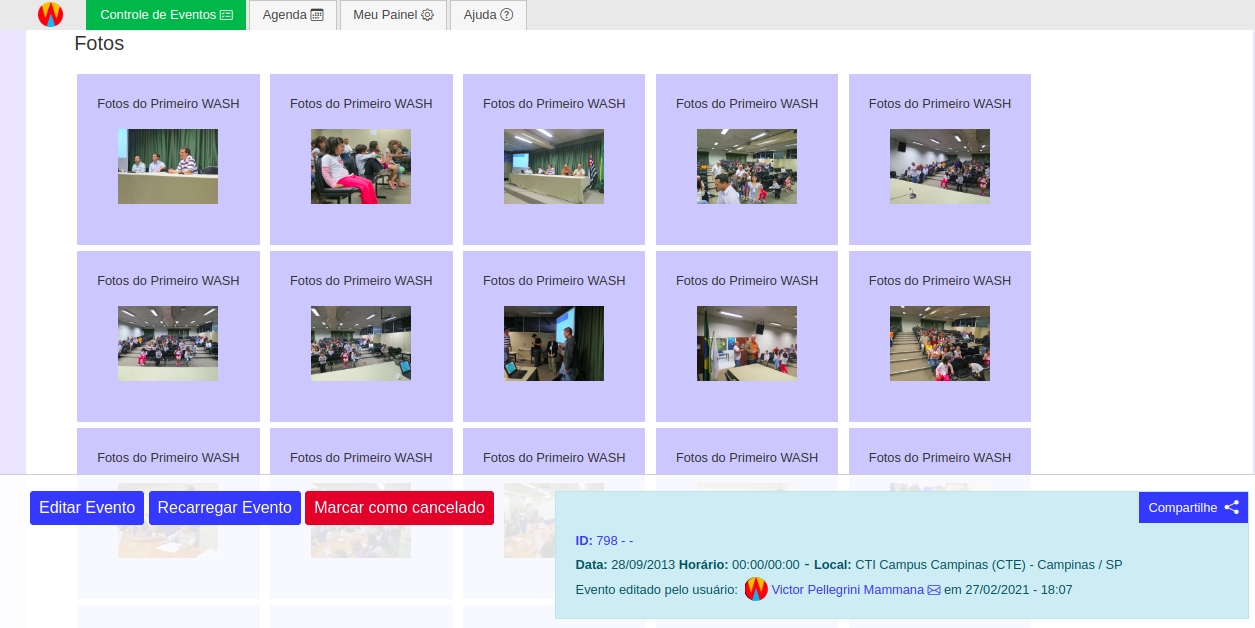
\includegraphics[max size={\textwidth}{\textheight}]{../../../imagens/primeiro-wash-corte.png}

	\end{center}

	\caption{\label{11f122f06c11abd40a3af9574514af9c30c712b9}Imagem da tela da plataforma Platuóxe, registro do primeiro evento do WASH realizado em 28 de setembro de 2013. (fonte: Plataforma Platuóxe)}

\end{figure}

O foco em "hackers" (ou "geeks") do primeiro evento indica que o público alvo, inicialmente, era constituído de jovens e adultos, com  poucas crianças. Esse fato explica, em parte, o nome do programa, que usou a palavra em português "aficionados" como tradução livre de "hackers" ou "geeks". Por diversas vezes, foi possível testemunhar as manifestações do coordenador do WASH lamentando a manutenção desse nome para um Programa que depois veio atender crianças (informação autorizada pelo coordenador). Entretanto, observamos que o "batismo" do Programa fugira ao controle de seus criadores, uma vez que o nome do WASH fora adotado também para os eventos com crianças que vieram depois, talvez, por sua sonoridade. Assim, " WASH " passou a ser a identidade do Programa, mesmo considerando que o acrônimo não reflete com precisão o que tem sido oferecido para os participantes, i.e., STEAM.

Esse fato, por si só, indica que, a rigor, a organização do primeiro evento não vislumbrava um programa educacional para a escola pública.

O caminho em direção a um Programa educacional para a escola pública foi sendo moldado ao longo de suas re-edições, que gradualmente passaram a atrair um público cada vez mais jovem, culminando no encontro definitivo de sua vocação, sintetizada em:


\noindent\begin{center}\mbox{\centering\fbox{\centering\par\parbox{0.7\linewidth}{\small\textit{"educação científica e tecnológica para o ensino fundamental, mediante protagonismo de jovens do ensino médio e superior" (Fonte: CNPq, 2020)}\normalsize}}}\end{center}


Ambicionando aplicar o que fora aprendido com avaliação pedagógica do OLPC, inclusive com a influência e colaboração da professora Dra.Afira Vianna Ripper que, como vimos, participara da referida avaliação, o WASH sempre buscou se vincular aos conceitos subjacentes ao pensamento de Papert.

Rapidamente, acompanhando a tendência mundial, o Programa se identificou com o STEM (Science, Technology, Engineering and Mathematics), adotando,também, as artes como um elemento fundamental de suas oficinas  (CNPq, 2020), fato que pode ser atribuído à influência do GESAC.

Como egressa do Programa GESAC, e ainda sem conhecer os conceitos construídos por outros (e.g. YAKMAN (2019), esta autora propôs a introdução das artes nas oficinas do WASH, aproximando-as das abordagens STEAM.

Essa mudança de "evento de hackers" para "evento STEAM" levou algum tempo para amadurecer e exigiu um compromisso maior com o conceito de método científico, requerendo do Programa a adoção de um "critério de demarcação" da ciência.

(CHIBENI, 2006) alerta para o fato de que "não há um método científico no sentido de uma receita universal para se fazer ciência", mas é possível identificar na ciência algumas especificidades em relação a outras formas de adquirir saber.

Os criadores do WASH, em vários pontos da documentação existente, mencionavam, inicialmente, o critério da falseabilidade de Popper como forma de verificar se uma proposição era científica ou não e; portanto, passível de fazer parte das atividades do Programa. Para isso, apresentavam a seguinte definição como sendo uma "forma simplificada de expressar o pensamento de Popper" (CNPq, 2020):


\noindent\begin{center}\mbox{\centering\fbox{\centering\par\parbox{0.7\linewidth}{\small\textit{"Falseabilidade - Todo conhecimento científico pode ser questionado e contestado, quando pode ser requerida a revisão de suas bases experimentais e teóricas. O conhecimento que não pode ser contestado, a exemplo da fé religiosa ou do ocultismo, não é um conhecimento científico." (CNPq, 2020).}\normalsize}}}\end{center}


É possível identificar na documentação do WASH o reconhecimento de que o critério da falseabilidade foi considerado como um "ponto de partida" para o trabalho de "demarcação de ciência e não-ciência", mas que para "os primeiros anos escolares é preciso resistir à tentação de ir muito além disso na busca por uma definição única e generalizada do método científico" (CNPq, 2020).

O que se identifica nas práticas do WASH, seja pela inspeção da documentação formal (relatórios), quanto pela busca dos temas de oficinas na plataforma "Platuóxe", é que nunca existiu uma preocupação em definir o conceito de método científico para as crianças, adotando como "divisa " a ideia simples de que "se você pode questionar, é ciência" (CNPq, 2020). Esta simplificação está de bom tamanho para os anos escolares iniciais, mas é claro que precisa se ampliar, com o amadurecimento.

A interação, o trabalho desenvolvido com o coordenador do Programa WASH, bem como a análise da documentação existente (CNPq, 2020)  (CNPQ, 2020a)  (MAMMANA et al., 2022a) mostram que existe uma predileção por uma definição bastante simples e direta de ciência, que é de fácil assimilação por todos os colaboradores:


\noindent\begin{center}\mbox{\centering\fbox{\centering\par\parbox{0.7\linewidth}{\small\textit{"Ciência é a compreensão que o outro constrói sobre o conhecimento de alguém" (Fonte: MAMMANA, V.P., CGEE (2010), pág. 48)}\normalsize}}}\end{center}


A frase acima foi primeiramente apresentada em (CGEE (2010), pelo coordenador do Programa WASH, tendo caráter original. O conceito subjacente é de que "não há ciência se não houver a compreensão por alguém dos conhecimentos gerados por outrem, mostrando que a ciência tem caráter social, sendo parte integrante da cultura de uma comunidade" (CNPq, 2020).

A forma como esse conceito é aproveitado no contexto da escola fundamental fica evidente na transcrição (CNPq, 2020), abaixo:


\noindent\begin{center}\mbox{\centering\fbox{\centering\par\parbox{0.7\linewidth}{\small\textit{"Na atuação do WASH junto aos primeiros anos escolares, há uma preocupação de estimular uma boa comunicação, seja através da preparação dos bolsistas para a multiplicação (oficinas), registro de resultados ou produção de audiovisual, por exemplo. Em outras palavras, é a preocupação com a capacidade de produzir narrativas calcadas num método." (Fonte: CNPq 2020)}\normalsize}}}\end{center}


Este estímulo à produção de narrativas, que facilitem a compreensão de algum conhecimento é, em última análise, o método científico do WASH. Através dele, a criança (ou jovem) é convidada a organizar o conhecimento adquirido, para que, através da conversão em um discurso, outros possam assimilá-lo e questioná-lo. Esta abordagem fica bem clara em ( WASH CNPq (2022):


\noindent\begin{center}\mbox{\centering\fbox{\centering\par\parbox{0.7\linewidth}{\small\textit{"(...) Outra atividade oferecida pelo WASH é a construção de discursos pelos participantes, muitas vezes na direção de uma produção audiovisual como ferramenta para o exercício de comunicação de suas descobertas e aprendizados. Nesse processo, são estimulados o planejamento, o debate de ideias, o trabalho em cooperação, a organização e algumas técnicas de produção audiovisual, embora este último aspecto seja mais instrumental. Tudo isso é feito de forma lúdica e dentro da zona proximal da criança." (Fonte:  WASH CNPq (2022)}\normalsize}}}\end{center}


Além da questão de disseminação do método científico para a escola pública, é possível identificar outras preocupações que levaram à formulação do WASH.

Na Fundamentação Teórica, mostramos a discrepância entre o investimento por hora, por aluno, no âmbito da escola pública em relação à escola privada (ver tabela 1). Este investimento mostra-se de 4 a 5 vezes maior para crianças matriculadas em escolas privadas de médio padrão em relação à escola pública, podendo chegar a 10 vezes mais para escolas privadas de alto padrão.

A situação fica mais crítica quando se consideram as oportunidades criadas pelas atividades de contraturno (CNPq, 2020b):


\noindent\begin{center}\mbox{\centering\fbox{\centering\par\parbox{0.7\linewidth}{\small\textit{"Alunos de escolas privadas tradicionais da cidade de São Paulo, por exemplo, chegam a ter várias dezenas de opções de atividades de contraturno que permitem enriquecer sua formação em áreas variadas, tais como: línguas estrangeiras, programação de computadores, Cultura Maker, STEAM, programação de jogos de computador, artes plásticas, música, modalidades esportivas, dança, expressão corporal, entre outras. Esta disparidade afeta principalmente os alunos de escolas públicas em regiões periféricas, que têm menos opções ainda para complementar sua formação." (Fonte:  CNPq, 2020b)}\normalsize}}}\end{center}


Na releitura do Documento de Referência do WASH, da qual esta que escreve é coautora, observamos que a preocupação em enfrentar essa disparidade sempre esteve presente no Programa. Em  (CNPq (2020b), é identificada, por exemplo, a preocupação com o início prematuro da vida profissional dos estudantes da escola pública, que acabam por interromper seus estudos, aprofundando o fosso em relação às oportunidades das crianças de famílias abastadas. Na mesma referência, é enfatizada a jornada de trabalho doméstico antecipada  das meninas, bem como dos cuidados com irmãos e irmãs menores, dificultando ainda mais o acesso, para as meninas, às mesmas oportunidades disponíveis aos estudantes do sexo masculino na mesma condição social.

Portanto, fica evidente a preocupação dos criadores do WASH com a " injusta diferença " existente entre estudantes de escolas públicas e privadas, que pode ter consequências duradouras para a inserção daquele indivíduo em sua própria cultura, prejudicando seu desempenho como cidadão ativo e próspero da sociedade" (CNPq, 2020b).


\noindent\begin{center}\mbox{\centering\fbox{\centering\par\parbox{0.7\linewidth}{\small\textit{"A principal contribuição que o Programa WASH busca dar é a construção de uma forma escalável para levar o STEAM à escola pública brasileira, respeitando suas peculiaridades, suas missões pedagógicas e seus valores culturais." (Fonte: CNPq, 2020)}\normalsize}}}\end{center}


O estudo das características do Programa WASH, por meio da documentação existente mostra, também, a preocupação de seus formuladores em concebê-lo de forma sustentável economicamente, visando valores por hora por aluno compatíveis com a capacidade de investimento do setor público  (CNPq, 2020b). Em várias ocasiões, o coordenador do WASH revelou que a criação da Plataforma Platuóxe teve como motivação principal a caracterização do custo por hora e por aluno.

Em termos práticos (CNPq, 2020), o WASH vem buscando as seguinte características para viabilizar a sua disseminação no sistema educacional brasileiro, sem a necessidade de vultuosos investimentos:


\begin{itemize}
\item "foco no investimento em pessoas e não em equipamentos, buscando aproveitar a infraestrutura existente;"
\item "busca por capilaridade, aproveitando a rede federal de ensino como elemento de regionalização do programa;"
\item "envolvimento de jovens estudantes como elementos de multiplicação, desenvolvendo o conceito do ensinar como pretexto para aprender;"
\item "uso de meios institucionais já existentes para a viabilização do financiamento do Programa, a exemplo da política de bolsas do CNPq, a indicação de emendas parlamentares diminuindo custos de gestão pela equipe;"
\item "criação de uma  "liturgia pedagógica," a partir de vivência, que permita sua reprodução nas várias localidades,sua adaptação às diferentes realidades em cada região;"
\item "renúncia ao conceito de curso;"
\item "renúncia ao conteudismo, oferta de pelo menos três atividades motivacionais que podem, ou não, serem adotadas localmente". Estas três etapas citadas em  [[CNPq (2020)]] referem-se às três oficinas de programação mais comuns do WASH: "Labirinto I", "Labirinto II" e "Space Invaders";
\item "demonstração de oficinas" como meio de capacitação dos multiplicadores, sempre com foco na
simplicidade de reprodução;"
\item "definição clara dos objetivos de cada vivência, sem exigência de pré-requisitos para a participação nas mesmas;"e
\item "estímulo para que as vivências encapsulem todo o conhecimento necessário para  atingir  seus objetivos, sempre que possível, de forma que o programa possa acolher todas as crianças, mesmo aquelas que não tiveram oportunidade de participar das experiências anteriores."
\end{itemize}

Para que essas características pudessem ser conquistadas dentro de um patamar de investimentos públicos viável, sem a criação de novas estruturas institucionais, os formuladores do WASH conceberam meios para aproveitar o investimento já feito em centros de excelência de pesquisa e educação, existentes no Brasil.

Inicialmente, pela própria origem profissional do coordenador do WASH, concebeu-se a ideia de estabelecer pontes diretas entre as Unidades de Pesquisa do Ministério de Ciência e Tecnologia e o ensino fundamental.

Nos primórdios do Programa, essa ideia não fora bem recebida, por alguns servidores do CTI Renato Archer, primeira instituição em que oficinas do WASH foram realizadas. Havia um receio de que tal atividade pudesse " desvirtuar " a missão de unidades que tinham a pesquisa como mote principal. Por envolver moradores de bairros de baixa renda, do entorno do CTI Renato Archer, percebia-se algum desconforto com a abertura da instituição para a comunidade nos finais de semana, para a realização das oficinas.

Para os críticos da ideia de receber crianças em unidades de pesquisa do Ministério, o coordenador do WASH, frequentemente, repetia um relato (testemunhado por esta autora) sobre sua experiência no Lawrence Berkeley Laboratory, na Califórnia, onde realizou a parte de pesquisa de seu trabalho de tese de doutorado:


\noindent\begin{center}\mbox{\centering\fbox{\centering\par\parbox{0.7\linewidth}{\small\textit{"Quando eu estava no Lawrence Berkeley Lab (LBL) eu me espantava com a presença de crianças circulando num instituto tão reputado e sério, com 13 prêmios Nobel. O LBL abria suas portas para eventos de educação científica para crianças de variadas idades. No CTI Renato Archer não recebíamos crianças. Talvez, esteja nos faltando recebê-las para conquistar  um prêmio Nobel para o Brasil." (fonte: interpretação autorizada de relato feito pelo coordenador do WASH em suas palestras).}\normalsize}}}\end{center}


Posteriormente, a este início restrito ao CTI Renato Archer, o WASH foi sendo levado para outros centros de excelência, tendo havido interesse imediato por parte do Instituto Federal de Educação, Ciência e Tecnologia de São Paulo-IFSP Campus Campinas.

A Fig. 28, obtida de uma apresentação do WASH de 2016, mostra um diagrama de como a ponte entre o ensino fundamental e os centros de excelência foi imaginada na fase inicial do Programa. Essa concepção está presente até os dias de hoje e foi cristalizada no Documento de Referência anexo à Portaria CTI 178/2018.



\captionsetup{format=plain}
\begin{figure}[htb]

	\begin{center}

		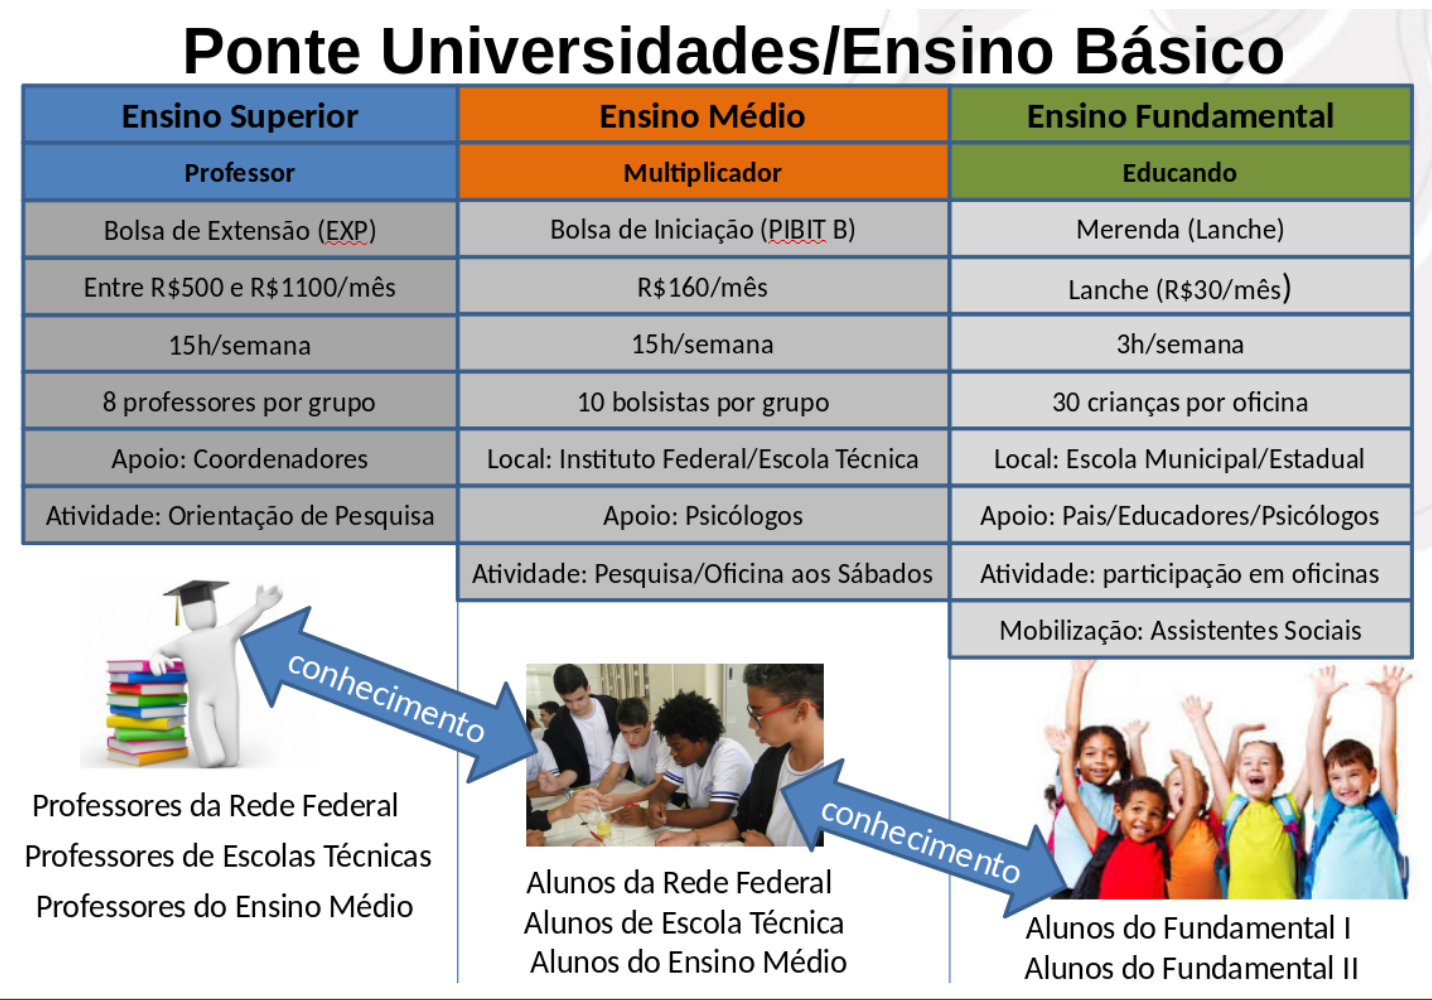
\includegraphics[max size={\textwidth}{\textheight}]{../../../imagens/ponte-wash.png}

	\end{center}

	\caption{\label{061843808cd4a78f12d61af45200969bc8abf5ca}Diagrama mostrando o conceito de ponte entre centros de excelência e o ensino fundamental, do WASH. (fonte: apresentação de divulgação do WASH)}

\end{figure}

O diagrama da figura mostra que a dita "ponte", uma metáfora para indicar relações entre instituições, está estruturada em três níveis:


\begin{itemize}
\item nível superior: educadores(as) do ensino superior, do ensino técnico e do ensino médio são convidados a orientar projetos de iniciação científica de alunos(as) do ensino superior, técnico e médio, com o compromisso de que uma parte do tempo do(a) aluno(a) seja dedicada para a realização de oficinas de disseminação da ciência no ensino fundamental;
\item nível médio, técnico e graduação: são oferecidas bolsas de iniciação científica para alunos (as) do nível médio de escolas públicas, bem como alunos (as) do nível superior e de escolas técnicas, cujos projetos serão orientados por educadores(as) do nível superior. O(a) aluno(a) do ensino médio, do ensino superior e das escolas técnicas que recebe bolsa se compromete a realizar oficinas no ensino fundamental, com o objetivo de disseminar conhecimentos aprendidos no WASH. As atividades com menores de idade são sempre supervisionadas por adultos(as) que tenham a  atribuição de responsabilidade pelos(as) menores de idade;e
\item nível fundamental: por meio de um processo de mobilização, são identificadas as escolas, organizações sociais que tenham interesse em disponibilizar as oficinas do WASH para suas crianças. O Documento de Referência anexo à Portaria CTI 178/2018 é o instrumento que dá os parâmetros de conduta para essa atividade, buscando torná-la proveitosa e segura para todos os partícipes.

\end{itemize}

Com esse trabalho, podemos dizer, de forma simplificada, que o WASH é um Programa de Iniciação Científica com uma característica especial: o aluno de iniciação assume o compromisso de multiplicar seus conhecimentos, participando como monitor de oficinas nas escolas de ensino fundamental ou outros tipos de instituições voltadas para educação de menores de idade.

Este entendimento se coaduna com as intenções declaradas na Portaria CTI 178/2018, que é o Documento de Referência do Programa:


\noindent\begin{center}\mbox{\centering\fbox{\centering\par\parbox{0.7\linewidth}{\small\textit{"São os bolsistas de iniciação científica, que executam projetos de pesquisa, coordenados pelos orientadores (as). Os projetos são desenvolvidos, durante a semana, no ambiente de  estudo e pesquisa (normalmente na Entidade Promotora). Os bolsistas atuam, também, como monitores dos educandos, sempre no contraturno da escola regular, através da realização de oficinas. As duas atividades (iniciação científica e monitoria) devem ocupar no máximo 15 horas semanais dos bolsistas." (fonte: Portaria CTI 178/2018);}\normalsize}}}\end{center}


O Programa WASH, como visionado na avaliação do PID, é substancialmente financiado por meio de emendas parlamentares do Legislativo Federal, seguindo a bem-sucedida experiência da Secretaria de Ciência e Tecnologia para a Inclusão Social- SECIS/MCT de financiar a inclusão social, entre 2005 e 2009, por recursos com origem externa ao MCT da época. Essa característica está explicitada na Portaria CTI 178/2018:


\noindent\begin{center}\mbox{\centering\fbox{\centering\par\parbox{0.7\linewidth}{\small\textit{"O presente Programa (WASH) é substancialmente mantido por recursos oriundos de emendas parlamentares, que disponibilizam recursos financeiros  para o pagamento da maior parte das bolsas. Anualmente, os deputados podem indicar as emendas para o Programa WASH. Para conquistar este apoio, o interessado deve enviar ao gabinete do Deputado um ofício apresentando o Programa, de forma a formalizar a solicitação de emenda." (fonte: Portaria CTI 178/2018)1}\normalsize}}}\end{center}


Identificamos 16 emendas aportadas ao WASH, as quais estão listadas na seção deste capítulo dedicada ao eixo 2.

As emendas, obtidas junto aos deputados federais, são direcionadas ao CNPq, que é o órgão responsável pelo financiamento dos projetos de pesquisa e extensão; e para cada emenda recebida é elaborado um projeto específico, como também indicado na Portaria CTI 178/2018:


\noindent\begin{center}\mbox{\centering\fbox{\centering\par\parbox{0.7\linewidth}{\small\textit{"Órgão Executor: Conselho Nacional de Desenvolvimento Científico e Tecnológico (CNPq), entidade ao qual são destinados os recursos provenientes de emendas parlamentares para custeio do Programa WASH." (fonte: Portaria CTI 178/2018)}\normalsize}}}\end{center}


Como estipulado pela Portaria CTI 178/2018, o Programa WASH estabelece papéis a serem desempenhados pelos participantes, como segue:


\begin{itemize}
\item Coordenador: "Servidor, professor, cientista ou pesquisador responsável pelo Programa WASH e interlocução junto ao CNPq, incluindo a elaboração do Plano de Trabalho do Projeto"  ([[CTI, 2018]]) . Este papel vem sendo desempenhado pelo Dr. Victor Pellegrini Mammana. Observa-se uma crescente delegação dessas tarefas para os partícipes mais experientes do Programa. Dentre as atividades que devem ser desempenhadas pelo coordenador estão: "inscrever e fazer gestão da Plataforma Carlos Chagas com as indicações das bolsas. É o responsável por solicitar prorrogação da execução da emenda se houver necessidade, buscar financiamento para o Programa."  ([[CTI, 2018]]) Além dessas responsabilidades expressas no termo de referência, observamos ao longo de nossa experiência outras, tais como: elaborar os relatórios para o CNPq, bem como a prestação de contas, com um minucioso trabalho de avaliação do desempenho de todos os bolsistas do projeto. Também, soma-se às demais atividades o papel de encontrar novas instituições interessadas em realizar o Programa, buscando novas parcerias, assim como novos parlamentares interessados em financiá-lo. Observa-se que estas atividades têm recebido apoio dos demais colaboradores do WASH.
\item Coordenador local: "Responsável por implementar o Programa junto aos interessados. Incluem-se dentre as suas atribuições: organizar e planejar as oficinas; preparar as reuniões das equipes locais; planejar e promover as oficinas de multiplicação com as crianças; elaborar com os orientadores e bolsistas os conteúdos/temas das oficinas; monitorar a elaboração conjunta pelos orientadores e bolsistas dos planos de trabalho específicos pelos orientadores e bolsistas, apresentando-os para o coordenador do programa junto ao CNPq; elaborar os relatórios de gestão do Programa; registrar a presença dos participantes;; organizar a participação dos educandos e bolsistas na Semana Nacional de Ciência e Tecnologia-SNCT e outros eventos similares."  ([[CTI, 2018]])
\item Monitor(a) ou Bolsista: " São os bolsistas de iniciação científica que executam projetos, de pesquisa coordenados pelos orientadores. Os projetos são desenvolvidos durante a semana, no ambiente de pesquisa (normalmente, na Entidade Promotora). Os bolsistas atuam, também, como monitores dos educandos, sempre no contraturno da escola regular, através da realização de oficinas. As duas atividades (Iniciação Científica e monitoria) devem ocupar no máximo 15 horas semanais dos bolsistas. Responsável por registrar os conteúdos das oficinas no site do MIT (Scratch) e demais instrumentos de registro."  ([[CTI, 2018]])
\item Orientador (a): "Responsável pela orientação científica e metodológica, tanto na elaboração quanto na execução dos planos de trabalho dos bolsistas/monitores, no Programa. Responsável pela participação em eventos de ciência e tecnologia (congressos, Semana Nacional de Ciência e Tecnologia) etc.
\item Educando: "Protagonista do fenômeno de aprendizagem. No presente contexto, o educando é o estudante do ensino fundamental que participa das oficinas." (CTI, 2018) Nossa experiência mostra que este papel é desempenhado, principalmente, por alunos do ensino fundamental.
\end{itemize}

Durante a experiência desta autora com a forma de executar o WASH no período anterior à pandemia de 2020, foi possível constatar que as oficinas se davam exclusivamente na forma presencial. Do ponto de vista formal, a Portaria CTI 178/2018 indica  a forma de realização das oficinas:


\noindent\begin{center}\mbox{\centering\fbox{\centering\par\parbox{0.7\linewidth}{\small\textit{"Oficina: Atividade de interação humana que envolve quantidade de pessoas pré-determinada, com duração fixa e data definida, executada por equipe composta por coordenador local, orientadores e monitores/bolsistas (ver adiante), com ênfase em conteúdo ou não, durante a qual busca-se o protagonismo do educando no processo de aprendizagem." (fonte: Portaria CTI 178/2018)}\normalsize}}}\end{center}


A ênfase dada pela Portaria CTI 178/2018 à "presença" dos partícipes nas "vivências", ou oficinas, nos permite depreender que o WASH foi concebido para ser exclusivamente presencial. Esta concepção gerou dificuldades para o Programa no auge do isolamento social, durante a pandemia, e esse é um dos pontos que precisa ser tratado na revisão do Documento de Referência do WASH.

No que tange à classificação das instituições partícipes, a Portaria CTI 178/2018 explicita os seguintes tipos:


\begin{itemize}
\item Órgão Executor: usando uma terminologia característica da gestão pública, o CNPq é o órgão executor do WASH, uma vez que executa o orçamento viabilizado pelas emendas parlamentares.
\item Órgão Coexecutor: também, no contexto da linguagem característica do setor público pode existir um órgão coexecutor dos recursos, papel que, na situação em que o projeto estava em 2018, era desempenhado pelo CTI Renato Archer. Essa situação não está mais presente, uma vez que o coordenador dos projetos CNPq associados ao WASH não está mais vinculado a aquela instituição, havendo que se rever esse aspecto no Documento de referência do Programa.
\item Entidade Promotora: "Instituição pública de educação ou pesquisa (federal, estadual ou municipal) cuja missão estatutária envolva a educação e/ou a disseminação da ciência, incluindo Instituições Científicas, Tecnológicas e de Inovação (ICTs)." ([[CTI, 2018]]). Na concepção do WASH, a experiência do CTI norteou muito a " liturgia " das atividades, havendo uma ênfase na realização das atividades no contraturno, situação em que era necessário oferecer transporte e alimentação para os participantes. Com a evolução do Programa, sua atividades foram sendo integradas ao turno escolar, requerendo menor ênfase no apoio ao transporte e alimentação, já oferecido pelas escolas partícipes (Entidades Responsáveis). Ao longo de uma década, muitos tipos de instituições desempenharam o papel de Entidades Promotoras: Institutos Federais (e.g. IFSP Campinas, IFSP Campos do Jordão, IFSP Jacareí, IFSP São José dos Campos, etc), Unidades de Pesquisa (CTI Renato Archer e CEMADEN), Universidades Estaduais (UNICAMP e USP), Universidades Federais (UFABC e UNIFESP), dentre tantas outras.
\item Entidade Responsável: na Portaria CTI 178/2018, a instituição responsável é "instituição pública (federal, estadual, municipal), ou entidades da sociedade civil sem fins lucrativos que tenham infraestrutura adequada para o oferecimento das oficinas."  ([[CTI, 2018]])  Com a evolução do Programa, decidiu-se por aceitar como entidades responsáveis apenas aquelas que tivessem, além da infraestrutura para as oficinas, a atribuição legal de responsabilidade pelos menos do ensino fundamental. Essa medida foi um aprimoramento da divisão de responsabilidades, garantindo que apenas profissionais habilitados e legalmente autorizados assumissem a responsabilidade de "cuidar de crianças". No formato inicial, na ausência de um profissional com essas características, era exigida a presença de pelo menos um responsável dos educandos, com a autorização dos demais, durante as oficinas. São exemplos de entidades responsáveis: as escolas municipais e estaduais, os sindicatos com escolas autorizadas (e.g. Dona Lindú), as igrejas, entre outras.
\end{itemize}

O WASH optou por não utilizar o instrumento de convênio para disseminar suas práticas nas entidades promotoras e responsáveis. O motivo é a lentidão do instrumento, Nossa experiência de gestão junto ao CTI Renato Archer, entre 2013 e 2018, quando esta autora foi secretária executiva da  diretoria, mostrou que o estabelecimento de um convênio entre entes federados pode levar meses; frequentemente, mais do que seis meses para ser assinado. Isso porque há várias instâncias pelas quais o processo administrativo deve passar, entre elas a AGU.

Um convênio é um tipo de "contrato" em que partícipes (e não partes) buscam um objetivo comum, estabelecendo direitos e obrigações. Avaliamos no início do Programa que este tipo de instrumento poderia ser dispensado se houvesse o cuidado de escolher entidades responsáveis que já tivessem em sua missão a educação, ao passo que houvesse, também, o cuidado de escolher entidades promotoras que já tivessem em sua missão a extensão. Para garantir a agilidade da disseminação, o WASH concebeu a ideia de "Documento de Referência", que deveria ser citado em um termo de adesão publicado pela entidade interessada em participar (promotora ou responsável). Por meio desta publicação seriam assumidos compromissos com a metodologia do WASH, sem a necessidade do Convênio, cabendo à entidade signatária arcar com os ônus dessa declaração pública. Essa ideia se mostrou bastante exitosa, como pode ser verificada pela lista de "termos de adesão" publicadas pelos partícipes do WASH (ver neste Capítulo a parte referente ao eixo 2).

\subsection[WASH na pandemia]{WASH na pandemia}\label{WASH na pandemia}
Vimos que o a Portaria CTI 178/2018 enfatiza a questão da "presença", ao descrever as vivências do WASH e, como testemunhado por esta autora, fato verificável pela Plataforma Platuóxe, o Programa não realizava atividades à distância antes da pandemia da covid.

Sabe-se que esse era um desígnio do coordenador do WASH, cujas declarações sobre a importância de manter o WASH como atividade presencial foram testemunhadas por todos os que participavam de reuniões de Coordenação ao longo dos vários anos do Programa. Justificava essa intenção pelo que tinha vivenciado nas visitas que fizera às oficinas promovidas por colaboradores de David Cavallo, em Massachussets, durante a avaliação do OLPC. David Cavallo era ativista do pensamento de Papert, contato de Afira Ripper no MIT e membro do OLPC, de Negroponte.

Na avaliação do PID (CGEE, 2010a), ficava clara a predileção do coordenador do WASH pelo conceito de educação como resultado da interação entre indivíduos. Na avaliação OLPC, ele indicava a dificuldade de representar digitalmente todos os aspectos da interação humana.

No entanto, a realidade da pandemia se impôs, impedindo a realização de atividades presenciais do Programa durante por mais de um ano. Já no primeiro semestre de 2020, assim que a gravidade da pandemia ficou evidente, foram tomadas medidas emergenciais para garantir a execução das emendas parlamentares, mesmo no contexto de isolamento social.

Duas iniciativas se estabeleceram imediatamente:


\begin{itemize}
\item Oficinas remotas assíncronas: o coordenador do Programa WASH iniciou experimentos utilizando o WhatsApp. Para isso contou com a iniciativa da Profa. Daniele de Souza Silva de experimentar uma nova forma de trabalho. A Profa. Daniele era da rede municipal de Educação da cidade de Jacareí, onde se desenvolveram os primeiros pilotos. A escola tinha poucos recursos, sem possibilidade de fornecer qualquer tipo de equipamento de informática aos estudantes, requerendo um modelo de oficina que pudesse ser realizado de forma assíncrona, utilizando o celular dos responsáveis (pais, mães, etc). A ideia era inverter a atividade de programação de jogos, atribuindo aos alunos a especificação do jogo, com a criação das personagens. A programação dos jogos, seguindo a especificação das crianças, seria feita em seguida, pelos bolsistas do WASH; também remotamente, uma vez que estes tinham mais acesso a computadores. A experiência, inicialmente limitada, resultou na produção de um jogo e audiovisuais, descrevendo o que estava sendo feito, com a participação dos educandos. Essa iniciativa foi depois aprimorada pelos bolsistas Michel Alencar Morandi e Ana Carolina de Deus Soares, tendo sido reproduzida em outras escolas.
\item "Ciência e Cultura, vamos brincar?"  (TOZZI, 2021): é uma websérie idealizada  e coordenada por essa  autora e produzida com o Movimento Nós Somos a Ciência e a Companhia Cultural Bola de Meia. A websérie resguarda o método científico e a cada episódio  busca  alinhar as temáticas cientificas às manifestações  da cultura popular.  Foram criados e produzidos audiovisuais em nível profissional, com diversas expressões e linguagens culturais  com a perspectiva de preservar a cultura da infância; e ao mesmo tempo,  cultivar práticas científicas.  Os educandos com seus familiares tiveram a oportunidade de usufruir de uma programação cientifica cultural para um público intergeracional. Neste trabalho, foi possível dar visibilidade às práticas STEAM do WASH,  às entrevistas com cientistas renomados, conteúdos tais como ciência, música, contação de histórias, quadros do tipo "faça você mesmo" e entrevistas. Essa programação foi denominada "Ciência e Cultura, Vamos Brincar?" (CCVB) e foi disponibilizada em vários meios (Youtube e TV Aberta). A Fig. 29 mostra o pedido de autorização para veiculação da websérie pela TVT. Outros pedidos semelhantes foram formulados. Foram nove episódios, os quais estão listados na parte destinada ao eixo 2 deste capítulo. Esta produção contou com a participação de uma ampla equipe, coordenada pela a autora. Os trabalhos foram concomitantes com o período em que esta autora esteve matriculada no mestrado, podendo ser considerados como um dos produtos educacionais da presente dissertação, razão pela qual é detalhada no capítulo de Produtos Educacionais.
\end{itemize}



\captionsetup{format=plain}
\begin{figure}[p]

\centering


\begin{minipage}[b]{0.4\linewidth}
        \centering
                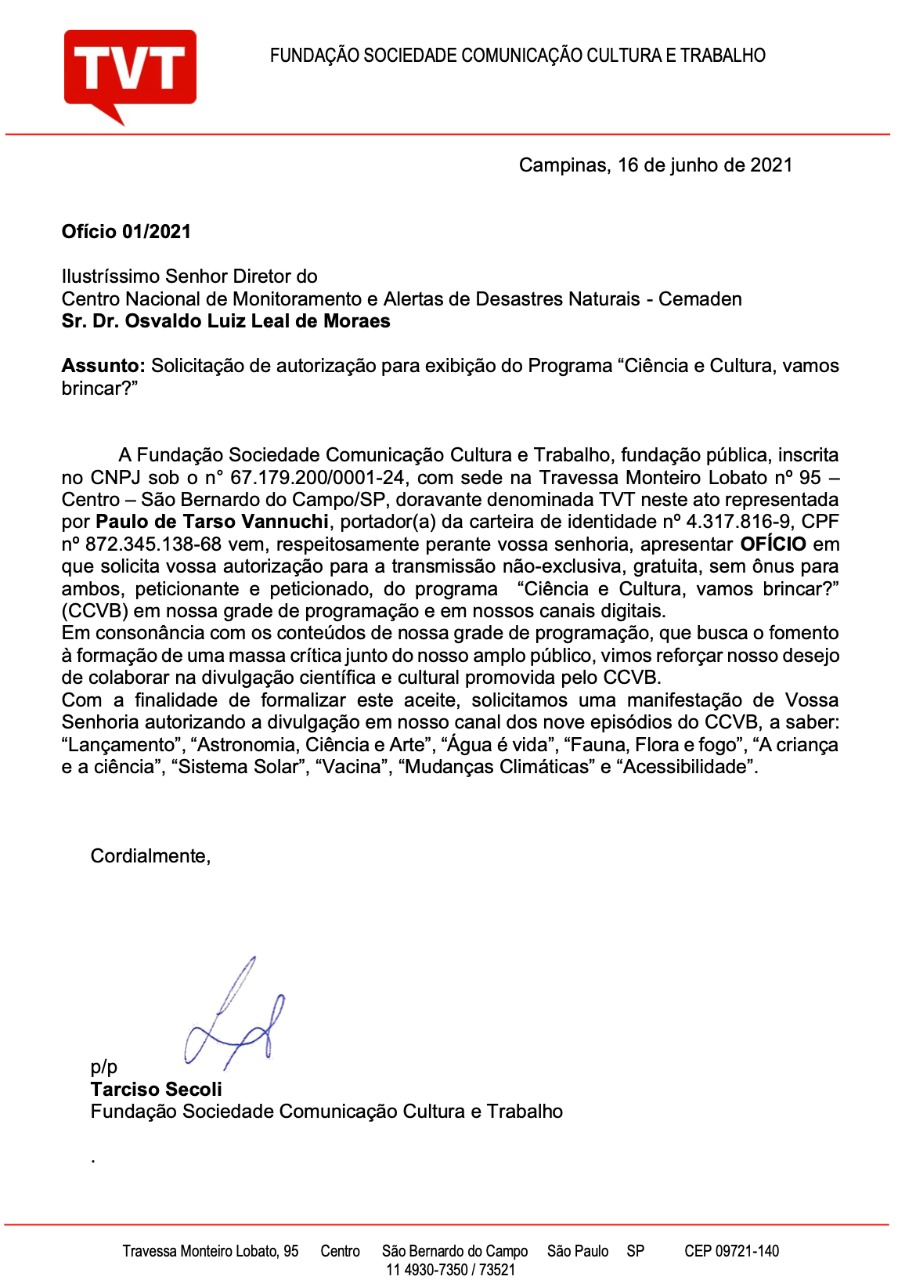
\includegraphics[width=1.0\linewidth]{../../../imagens/TVT.jpg}
                \caption{Documento de solicitação de autorização para a veiculação da websérie Ciência e Cultura, vamos brincar?, exemplificando o interesse de TVs-web e abertas pela programação criada pelo WASH. (fonte: acervo do WASH)}
                \label{51f9418c1ca6e2404e9d774513fb6c023d10b3bb}
\end{minipage}%
\hspace{0.5cm}
\end{figure}



A introdução de atividades remotas no WASH, como resultado da experiência da pandemia, é uma das justificativas para a revisão do documento de referência.

\section[Caracterização dos Indicadores do WASH (eixo 2)]{Caracterização dos Indicadores do WASH (eixo 2)}\label{Caracterização dos Indicadores do WASH (eixo 2)}
Na seção da Fundamentação Teórica, embasamos os conceitos de "dados", "informações" e "conhecimento"  através da referência (SETZER  e SILVAS, 2017). Traçando um paralelo com aqueles conceitos, podemos dizer que o objetivo da realização de consultas estruturadas, via Plataforma "Platuóxe", é produzir informações, na forma de indicadores, os quais, analisados e interpretados, levarão à produção dos conhecimentos sobre objeto de estudo. Estes conhecimentos permitirão avaliar as Hipóteses 1, 2, 4, 5 e 6.

Considerando os conceitos definidos na seção 2.3, da Fundamentação Teórica (eventos, emendas parlamentares, planos de trabalho, relatórios e iniciação científica), são exemplos de indicadores a serem apresentados nesta seção:


\begin{itemize}
\item quantidade de emendas parlamentares concedidas ao WASH;
\item quantidade de termos de adesão ao WASH;
\item estimativa do número de pessoas atendidas;
\item evolução temporal do número de pessoas atendidas (participações);
\item participantes por sexo (indicador de equidade);
\item número de bolsistas;
\item temas nos planos de trabalho e relatórios das iniciações científicas;
\item quantidade de eventos realizadas;
\item perfil etário dos participantes em eventos;
\item distribuição de temas nos eventos;
\item distribuição das atividades nos eventos;
\item quantidade de cidades atendidas; e
\item produção audiovisual.
\end{itemize}

Importante registrar que os indicadores foram obtidos a partir da contribuição de vários colaboradores do WASH, que elaboraram os códigos em SQL, para as consultas estruturadas, a partir de nossa especificação.

Entretanto, o trabalho de produção de indicadores não se restringiu à " Platuóxe" e outras três fontes de dados foram utilizadas:


\begin{itemize}
\item Plataforma de Planejamento Financeiro do Programa WASH: instrumento para acompanhamento das concessões de bolsas, seus prazos e validades, documentos de outorgas e planos de trabalho. Trata-se de uma ferramenta de compliance e prestação de contas de cada projeto, mas que, também, pode ser usada para a caracterização dos mesmos, pela abrangência dos dados nela contida;
\item Planilhas eletrônicas: construídas  manualmente para viabilizar a verificação dos dados das demais plataformas, uma vez que foram identificadas algumas fragilidades nas demais fontes de informações; e
\item Acervo de documentos usados também no âmbito do eixo 1 (história), bem como plataformas de entidades públicas, a exemplo da Plataforma Carlos Chagas do CNPq (CHAGAS, 2022).
\end{itemize}

Dois recortes temporais foram adotados, como já explicitado em Materiais e Métodos:


\begin{itemize}
\item Recorte A da Platuóxe, de setembro de 2013 a agosto de 2022 (congelada); e
\item Recorte B da Platuóxe, de setembro de 2013 a janeiro de 2023 (alimentada em tempo real).
\end{itemize}

\subsection[Lista de Emendas Parlamentares concedidas]{Lista de Emendas Parlamentares concedidas}\label{Lista de Emendas Parlamentares concedidas}
No eixo 1, identificamos que o WASH tem como fonte de financiamento principal as emendas parlamentares do Legislativo Federal, mas a lista completa ainda não foi apresentada.

Para levantar as listas, usamos como fonte a Plataforma Carlos Chagas do CNPq (CHAGAS, 2022), sendo possível constatar a existência das seguintes emendas concedidas ao WASH:


\begin{itemize}
\item "Programa WASH, emenda concedida pelo Deputado Federal Ivan Valente, em 2016;
\item "Programa WASH!", emenda concedida pelo Deputado Ivan Valente, em 2017;
\item "Formação em Captura de Movimentos", emenda concedida pelo Deputado Federal Alex Canziani, em 2018;
\item "Cinema de animação 3D e desenvolvimento de jogos com a ferramenta Blender e o Programa WASH", emenda concedida pelo Deputado Alex Canziani, em 2019;
\item "Programa WASH no Paraná", emenda concedida, em 2020, pelo Deputado Alex Canziani;
\item "Programa WASH-STEAM no Estado de São Paulo: Promoção da Ciência, Tecnologia, Engenharia, Artes  e Matemática na Rede Pública de Ensino", emenda concedida pelo Deputado Federal, Ivan Valente, em 2020;
\item "Regiões Metropolitanas", emenda parlamentar concedida, pelo Deputado Federal Alexandre Padilha, em 2020;
\item "Redes de Aprendizagem", emenda concedida, em 2020, pelo Deputado Federal Ivan Valente;
\item "Programa WASH - Lei Aldir Blanc", emenda parlamentar concedida, pelo Deputado Federal  Ivan Valente, em 2020;
\item "Programa WASH em Campos do Jordão", emenda parlamentar concedida, pelo Deputado Federal Eduardo Cury, em 2020;
\item "Programa WASH no ABC", emenda parlamentar concedida, pelo Deputado Federal Vicentinho em 2022;
\item "WASH na USP", emenda parlamentar concedida; pelo Deputado Federal Orlando Silva, em 2022;
\item "WASH na UFABC", emenda parlamentar concedida, pelo Deputado Federal Alexandre Padilha, em 2022;
\item "WASH em São Bernardo do Campo", emenda concedida, pelo Deputado Federal Carlos Zaratini, 2022 e
\item "Projeto Renato Archer", emenda concedida, pelo Deputado Federal Ivan Valente, em 2022.
\end{itemize}

\subsection[Lista de Termos de Adesão ao Programa WASH]{Lista de Termos de Adesão ao Programa WASH}\label{Lista de Termos de Adesão ao Programa WASH}
O WASH decidiu-se por não estabelecer o instrumento de Convênio como meio de disseminação do Programa. Essa decisão foi decorrente do prazo excessivo para tramitação desse tipo de instrumento jurídico, que pode demorar vários meses. Alternativamente, concebeu-se um formato de mobilização de outras instituições, baseado na adesão por declarações  unilaterais, denominadas "adesões".

Combinando a busca na "Platuóxe" com a busca no cervo, identificamos os seguintes tipos de documentos de adesão:  edição de portarias, termos de adesão, boletins, atas deliberativas de reuniões de conselhos de escolas e de saúde, manifestações por ofícios, enfim: documentos editados pelas entidades interessadas no Programa, que se configuram como atos de gestão.

Abaixo, apresentamos, organizadas por tipos de instituições, as adesões encontradas pela autora, nos registros do WASH.

No que se refere a "unidades de pesquisa", identificamos os seguintes documentos:


\begin{itemize}
\item Centro de Tecnologia da Informação Renato Archer - CTI - proponente inicial da metodologia, por meio da Portaria CTI 178/2018, como já amplamente mencionado ao longo do texto:
\item CEMADEN - Portaria No. 144/2019/SEI-CEMADEN, de 02/12/2019 - Institui o Programa CEMADEN Educação, define sua estrutura e formas de implementação, e dá outras providências. A Portaria traz em seu Art 3º.: O Programa CEMADEN EDUCAÇÃO adotará como uma de suas formas de execução o termo de referência do Programa WASH - Workshop Aficionados em Software e Hardware, conforme consta do Anexo I da Portaria, n° 178/2018/SEI-CTI, de 12 de novembro de 2018, promovendo a integração das temáticas de ciência, tecnologia, matemática, arte e engenharia, inerentes a aquele Programa, com as demais características e temáticas do CEMADEN EDUCAÇÃO, realizando adaptações didáticas quando couber, conforme previsto no Anexo, I desta Portaria.
\end{itemize}

Na esfera municipal, identificamos  várias formas de adesão do Poder Executivo. Os casos mais emblemáticos são aqueles que se deram pela aprovação de leis municipais, como ocorreu nas cidades de Prado Ferreira e Dr. Camargo, no Estado do Paraná. Nestas duas iniciativas independentes, identificamos o protagonismo de duas autoridades públicas com grande comprometimento com a educação em suas cidades, o então prefeito, Silvio Damasceno, de Prado Ferreira; e a vereadora, Valdirene Maria dos Santos (Dila)  de Dr. Camargo. Nas demais cidades, observamos a utilização dos instrumentos de portaria, normalmente editada pelas secretarias de educação. A participação de Campinas, que envolveu o Observatório Municipal, foi o único caso de utilização de convênio, como se vê na lista, a seguir:


\begin{itemize}
\item Jacareí/SP- Secretaria Municipal de Educação - Portaria 3865, de 20/02/2020. Adota a Metodologia do Programa WASH nas atividades pedagógicas da Secretaria Municipal de Educação de Jacareí (Publicada no Boletim Oficial do Município de Jacareí, em 21/02/2020);
\item Município de Drº Camargo - Lei nº 1601 de 2021-Institui a metodologia WASH como política pública no município paranaense, Dr. Camargo. Link: http://www.doutorcamargo.pr.gov.br/
\item Município de Prado Ferreira-Lei nº 496, de 16 de abril de 2019-Institui o Programa Profissão 4.0 para a capacitação e orientação profissional destinadas às crianças, jovens e adultos do município de Prado Ferreira/PR.
\item Secretaria Municipal de Cultura de Campinas-Convênio com o Observatório Municipal Jean Nicolini, 2018:
\item Secretaria Municipal de Santo Inácio/ PR-Oficializa a adesão ao Programa WASH em, 20/12/2021;
\end{itemize}

Foram identificadas adesões das seguintes universidades federais/estaduais e Institutos Federais:


\begin{itemize}
\item Universidade de São Paulo-USP- Portaria GR 7669, de 8/07/2021- Estabelece as condições para a execução do Programa WASH na Universidade de São Paulo;
\item Universidade Tecnológica Federal do Paraná-UTFPR - Portaria do Diretor Geral nº 147, 05/11/2020 - Adota a Portaria 178/2018/SEI/CTI, de 12/11/2018 como modelo de referência do Programa WASH, criando condições para que a UTFPR, atue como entidade promotora;
\item Fundação Universidade Federal do ABC -Portaria 915/2020, DE 27/08/2020- Adota o Programa WASH na UFABC, publicada no Boletim de Serviço no. 977, em 28/08/2020;
\item Instituto Federal Jacareí/SP - Portaria JCR.0031/2019 - abril de 2019 - Institui o Programa WASH no Campus Jacareí;
\item Instituo Federal Campus Londrina/PR - Portaria 101, de 22/04/2019 - Adota a Portaria 178/2018/SEI/CTI, de 12/11/2018, como modelo de referência do Programa WASH, para que o IF-PR atue como entidade promotora;
\item Instituto Federal Campina/SP - Portaria CMP 0043/2019, de 24/04/2019 - Institui o Programa WASH no Campus Campinas;
\item Instituto Federal Sorocaba/SP - Portaria SOR .0027/2019 - 25 abril de 2019 - Institui o Programa WASH no IFSP, Campus Sorocaba;
\item Instituto Federal Araraquara/SP - Portaria no ARQ. 0042/2019, de 25 de abril de 2019 - Institui o Programa WASH no Campus Araraquara do IFSP;
\item Instituto Federal Salto/SP, Portaria SLT - 0061/2019 - de 06 de maio de 2019 - Institui o Programa WASH no Campus Salto;
\item Instituto Federal Cubatão/SP Portaria CBT 055/2019 - de 27 de maio de 2019 - Institui o Programa WASH no Campus Cubatão;
\item Instituto Federal São José dos Campos/SP Portaria  SJC. 0083/2019, de 10/06/2019 - Designa membros para o Grupo de Trabalho para Programa WASH;
\item Instituto Federal Campos do Jordão/SP, Portaria CJO 0109/2019, de 16/10/2019- Designar membros para o programa WASH; e
\item Instituto Federal Caraguatatuba/SP, Portaria 95/2021 DRG/CAR/IFSP, 25 de Novembro de 2021 - Designar o servidor Nelson Alvez Pinto para coordenar o Grupo de Trabalho (GT) para adoção da Metodologia WASH, no Campus de Caraguatatuba.
\end{itemize}

Foram identificadas as adesões formais das seguintes escolas estaduais:


\begin{itemize}
\item E.E. Ernesto Monte - Bauru/SP
\item E.E. Expedito Camargo Freire - Campos do Jordão/SP
\item E.E. Prof. Sebastião Inoc Assumpção - Arealva/SP
\item E.E. Profa. Fanny Monzoni Santos - Osasco/SP
\item E.E. Prof. Hadia Feres - Carapicuíba/SP
\item E.E. Dr. Álvaro de Souza Lima - São Paulo/SP
\item E.E. Dinah Lúcia Balestreiro - Brotas/SP  
\item E.E. Prof. Walmar Lourenço Santiago - São José dos Campos/SP
\item E.E. Rubens Moreira da Rocha- Santo André/SP
\item E.E. Professora Cecília Pereira - Campinas oficializa adesão ao Programa WASH, por meio de ofício 112/2018, em 23/08/2018
\item E.E. Professora Lourdes Maria de Camargo - São José dos Campos/SP oficializa adesão à metodologia do Programa WASH; em 24/09/2021
\item E.E. Sebastião de Oliveira Rocha - São Carlos/SP
\item E.E. Prof. Juvenal Machado de Araújo - São José dos Campos, adesão à metodologia do Programa WASH, em 14/09/2021
\item E.E. Vitor Meireles - Campinas/SP, oficializa a adesão à Metodologia do Programa WASH, por meio da apreciação e aprovação do Conselho de Escola, em reunião realizada no dia  04/09/2020 .
\item E.E Prof. Mauro de Oliveira - São Paulo/SP, oficializa adesão à metodologia do Programa WASH, em 08/04/2021
\end{itemize}

Foram identificadas adesões das seguintes escolas técnicas estaduais:


\begin{itemize}
\item ETEC Irmã Agostina - São Paulo/SP
\item ETEC Gildo Marçal Bezerra Brandão - São Paulo/SP
\item ETEC Prof Marines Teodoro de Freitas Almeida - Novo Horizonte/SP oficializa adesão à metodologia do Programa WASH, na data de 29/11/2021
\item ETEC Takashi Morita - São Paulo/SP
\item ETEC Francisco de Abreu - São Paulo/SP e
\item ETEC Ten. Aviador Gustavo Klug - Pirassununga/SP
\end{itemize}

Foram identificadas adesões das seguintes escolas municipais de ensino fundamental:


\begin{itemize}
\item EMEF Tancredo Neves - Campos do Jordão/SP
\item EMEI Profa. Édera Irene Pereira de Oliveira Cardoso - São José dos Campos/SP
\item EMEF Roberto Alves Lima Júnior- Londrina PR, adesão em 12/04/2021
\item EMEF Maestro Roberto Pereira Panico- Londrina/ PR
\item EMEF PROF Clotilde Barraquet Von Zuben - Campinas/SP oficializa adesão à metodologia do Programa WASH, em 19/04/2022
\item EMEF Professora Maria Regina Cachuté- Jacareí/SP, adesão à metodologia do Programa WASH , em 10/11/2021
\item EMEF Luiz Gonzaga do Nascimento Júnior-São Paulo/SP, oficializa adesão à metodologia do Programa WASH em 03/09/2021
\item E.M. Tancredo Neves - Dr. Camargo/PR
\item E.M. Padre Mateus Elias - Dr. Camargo/PR
\item E.M. Helena Kolody - Prado Ferreira/PR, oficializa adesão à metodologia do Programa WASH em 21/06/2022
\item E.M. Amadeu Carletti Junior - Campos do Jordão/SP, oficializa adesão à metodologia do Programa WASH em 19/05/2022
\item E.M. Dr. Antônio Nicola Padula - Campos do Jordão/SP, oficializa adesão à metodologia do Programa WASH,  em 22/10/2021
\item E.M. Professora Lucília Florence Cerquera, adesão em maio de 2022.
\item EMEIF Professor Luiz Carlos Maiola Covre - Jacareí/SP oficializa adesão à metodologia do Programa WASH, em 12/10/2021
\item EMEFI -  Padre Francisco e Silva - Campinas/SP.
\item Colégio Técnico de Lorena Prof. Nelson Pesciotta - Lorena/SP e
\item Colégio  Estadual Acqua Ville, ensino fundamental e  médio.  Oficializa adesão a metodologia do Programa WASH ,em 09/02/2022
\end{itemize}

Foram identificadas as adesões das seguintes organizações sociais e sindicatos:


\begin{itemize}
\item Sindicato dos Metalúrgicos do ABC
\item Instituto Sócio Cultural Voz Ativa- Campinas/SP,  parceria com o Programa WASH, em 01/02/2019
\item MSTL - Movimento Sem Terra de Luta - São Bernardo do Campo/SP
\item FUNBOSQUE - Fundação Centro de Referência em Educação Ambiental Escola Bosque Eidorfe Moreira, São João do Outeiro, Belém do Pará
\end{itemize}

Foram identificadas as adesões das seguintes ações na área de saúde:


\begin{itemize}
\item UNICAMP - CIN (Centro Integrado de Nefrologia) - Campinas/SP, oficializa adesão à metodologia do Programa WASH, em 24/05/2022
\item Conselho Municipal de  Saúde de Campinas - Termo de Adesão e Compromisso de 14/07/2021 - Oficializa a adoção da Metodologia WASH/STEAM como meio de disseminação de conhecimentos com base científica, principalmente na área de saúde.
\item Comunidades Pico do Jaraguá e Heliópolis - São Paulo/SP
\end{itemize}

Os dados apresentados indicam a existência de documentos de adesão editados por cerca de 66 instituições diferentes. Sabe-se que o número acumulado de instituições participantes é maior, dado que, ao longo de 10 anos, ocorreram muitos eventos em instituições e cidades, sem que os interessados publicassem um documento de adesão.

\subsection[Quantidade e qualidade dos registros na amostra do público atendido]{Quantidade e qualidade dos registros na amostra do público atendido}\label{Quantidade e qualidade dos registros na amostra do público atendido}
Iniciamos explicitando que parte dos indicadores apresentados neste capítulo de Resultados, principalmente aqueles levantados com base na Platuóxe, foram obtidos por amostragem, uma vez que identificamos que o WASH não tem os instrumentos para coletar os dados de participantes integralmente.

Tal limitação, discutida no capítulo de Materiais e Métodos, está relacionada à falta de atribuição legal para que o Programa colete, por si só, dados cadastrais de seus participantes, tornando-o dependente do registro e disponibilização destas informações pelas entidades parceiras (promotoras e responsáveis).

Identificamos, também, um outro motivo que ocorreu mesmo quando as restrições de registro não estavam presentes. Observamos o não cumprimento das diretrizes do WASH especificadas no documento de referência - ver "descrição de uma oficina" em (CTI (2018) - situação que, em alguns casos, se deu por inação dos próprios colaboradores do WASH, que deveriam relembrar o responsável presente sobre a importância de elaboração da lista de presença, com nome e data de nascimento.

Portanto, tem ocorrido, frequentemente, a falta de registro na Platuóxe dos participantes que estão sob custódia da Entidade Responsável.

A situação se intensificou a partir da edição da Lei Geral de Proteção de Dados (LGDP). Tudo indica que as vedações dessa lei, impostas aos gestores escolares, têm aumentado a resistência, por parte dos parceiros, em compartilhar informações dos estudantes, mesmo quando as listas de presença foram registradas na entidade responsável.

Tais fatos indicam que o registro de presença precisa ser mais enfatizado na re-edição do Documento de referência do Programa WASH, que também precisa apresentar uma solução melhor adaptada à nova realidade da LGPD.

Os indicadores, aqui, apresentados referem-se ao Recorte A, de setembro de 2013 a agosto de 2022.

Para conhecer o número de cadastros na base de dados, que representam a amostra do público atendido, é preciso fazer uma consulta sobre a tabela "participantes2", que é a parte da base de dados relacional que contém os cadastros. Essa consulta é feita por meio da linguagem SQL, já descrita na Fundamentação Teórica e nos Materiais e Métodos.

O uso da linguagem SQL escapa ao escopo imediato deste trabalho, razão pela qual será omitido aqui o comando específico utilizado.

O resultado obtido com a consulta SQL, para os dados congelados em 26 de agosto de 2022 (Recorte A), foi de 3.312 (três mil,trezentos e doze) participantes.

Entretanto, uma inspeção da lista de participantes no âmbito desta pesquisa indicou que há cadastros repetidos; situação resultante, provavelmente, de erros de digitação.

Felizmente, a linguagem SQL permite excluir os cadastros repetidos, tarefa que foi delegada à equipe de TI do WASH. Para isso, foi construída uma nova consulta com a palavra reservada "distinct", que resultou em um número um pouco menor de participantes: 3.265 (três mil duzentos e sessenta e cinco) pessoas, agora sem repetições.

O conjunto de 47 pessoas representa a diferença entre 3.312 e 3.265 participantes, e pode conter duas situações:


\begin{itemize}
\item cadastros indevidamente repetidos (por erro de digitação ou operação), referentes à mesma pessoa; e
\item homônimos.
\end{itemize}

Aplicamos, com apoio da equipe de TI do WASH, algumas variantes das consultas SQL para identificar, caso a caso, qual das duas situações estava presente. Com isso, pudemos concluir que os cadastros repetidos não se referiam a homônimos, evidência de que a opção (a) acima é a mais provável. Consequentemente, 3.265 participantes é o número que melhor representa o tamanho da amostra de cadastrados registrada na plataforma Platuóxe,  com um erro de cerca de 1,4\% nos registros totais (47 repetições). Este número de erros é relativamente pequeno para o universo de participantes. Os 47 registros repetidos foram excluídos para a geração dos demais indicadores no contexto do Recorte A.


\noindent\begin{center}\mbox{\centering\fbox{\centering\par\parbox{0.7\linewidth}{\small\textit{A amostra de participantes do WASH, registrada na plataforma Platuóxe, é constituída de 3.265 participantes.}\normalsize}}}\end{center}


Um outro aspecto que precisa ser bastante enfatizado é que o número efetivo de participantes no WASH deve ser substancialmente maior do que a amostra de 3.265 cadastrados.

Para sustentar esta afirmação, é possível considerar que muitas oficinas do Programa, principalmente as que ocorreram em ambientes abertos foram realizadas sem registro de presença  de entrada, impedindo que o cadastro individualizado de participantes fosse feito.

Mas, esta afirmação não teria validade se não fosse possível apresentar evidências de que eventos ocorreram com as características citadas acima. Ou seja, precisamos mostrar casos em que o número de participantes foi maior do que o efetivamente cadastrado.

Desta forma, passamos a apresentar exemplos de eventos em que tal situação ocorreu, verificando, de forma não exaustiva, que existiram pelo menos sete eventos de grande porte em que o número de registrados na plataforma não refletiu o que está presente nos registros fotográficos. Parece-nos que a descrição de sete eventos nessa situação é suficiente para comprovar nossa afirmação:


\begin{itemize}
\item evento de grande porte realizado no CTI Renato Archer, ocorrido em 11 de abril de 2015, quando centenas de crianças participaram da apresentação do "Ciência em Show". Os registros oficiais indicam a presença de cinco pessoas, o que não se coaduna com os registros fotográficos, que indicam um público entre 150 e 200 pessoas (ver Fig. 30);
\item comemoração do dia das crianças realizada em 3 de outubro de 2015, no CTI Renato Archer com atividades musicais e culturais. Os registros da plataforma, neste dia, apontam para a participação de nove participantes, mas os registros fotográficos do evento apontam para uma presença muito superior (ver Fig. 31).
\item Evento de confraternização de Natal, realizado no CTI Renato Archer, com palestras e outras atividades lúdicas, realizado em 19 de dezembro de 2015, com oito participantes, mas os registros fotográficos indicam a participação substancialmente maior de crianças (ver Fig. 32).
\item Evento Greenk, patrocinado pelo MCT, que aconteceu no Expo Center Norte Anhembi, em São Paulo, na semana de 27 de maio de 2018. O porte do evento e número de dias de realização indicam uma quantidade  maior do que o registrado (13 pessoas). Essa discrepância se deu porque o tipo de evento não permitia o cadastro de público, ficando os registros restritos aos bolsistas multiplicadores, bem com aos demais responsáveis (ver Fig. 33).
\item Em 23 de junho de 2018 o Programa WASH promoveu uma visita ao Museu Aberto de Astronomia- MAAS, em Campinas. Os registros oficiais não trazem o número de participantes, mas os registros fotográficos indicam a presença de várias dezenas de crianças (ver Fig. 34);
\item Evento em praça pública realizado na cidade de Prado Ferreira/PR, em 31 de maio de 2019, para o lançamento do Programa WASH no âmbito do Projeto Municipal Profissão 4.0. Foi possível estimar uma presença de centenas de pessoas, com a praça tomada pelo público (ver Figs. 35); e
\item Evento Dia da Família na Escola, realizado na EMEF Milton Pereira Costa, em São Miguel Paulista, no dia 27 de novembro de 2022. Mediante ofício da Diretoria da escola, o Programa WASH foi informado que o público foi de cerca de 300 pessoas. Na Platuóxe não consta o registro de presenças nesse dia.
\end{itemize}



\captionsetup{format=plain}
\begin{figure}[p]

\centering


\begin{minipage}[b]{0.4\linewidth}
        \centering
                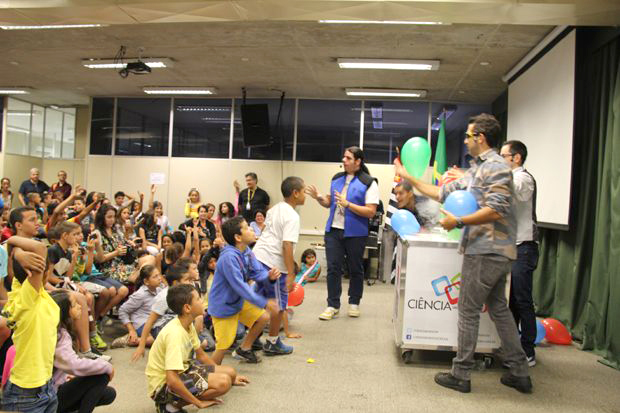
\includegraphics[width=1.0\linewidth]{../../../imagens/Evento-Ciencia-Em-Show.jpg}
                \caption{Evento científico e cultural do WASH, realizado no CTI Renato Archer, em 11 de abril de 2015, com a participação do Ciência em Show. O caráter amplo do evento não permitiu controlar a presença de participantes que pôde ser estimada em perto de duas centenas de crianças. (acervo da autora).}
                \label{5340059e38852932c32c5ce8624858fef8a1f3f0}
\end{minipage}%
\hspace{0.5cm}
\begin{minipage}[b]{0.4\linewidth}
        \centering
                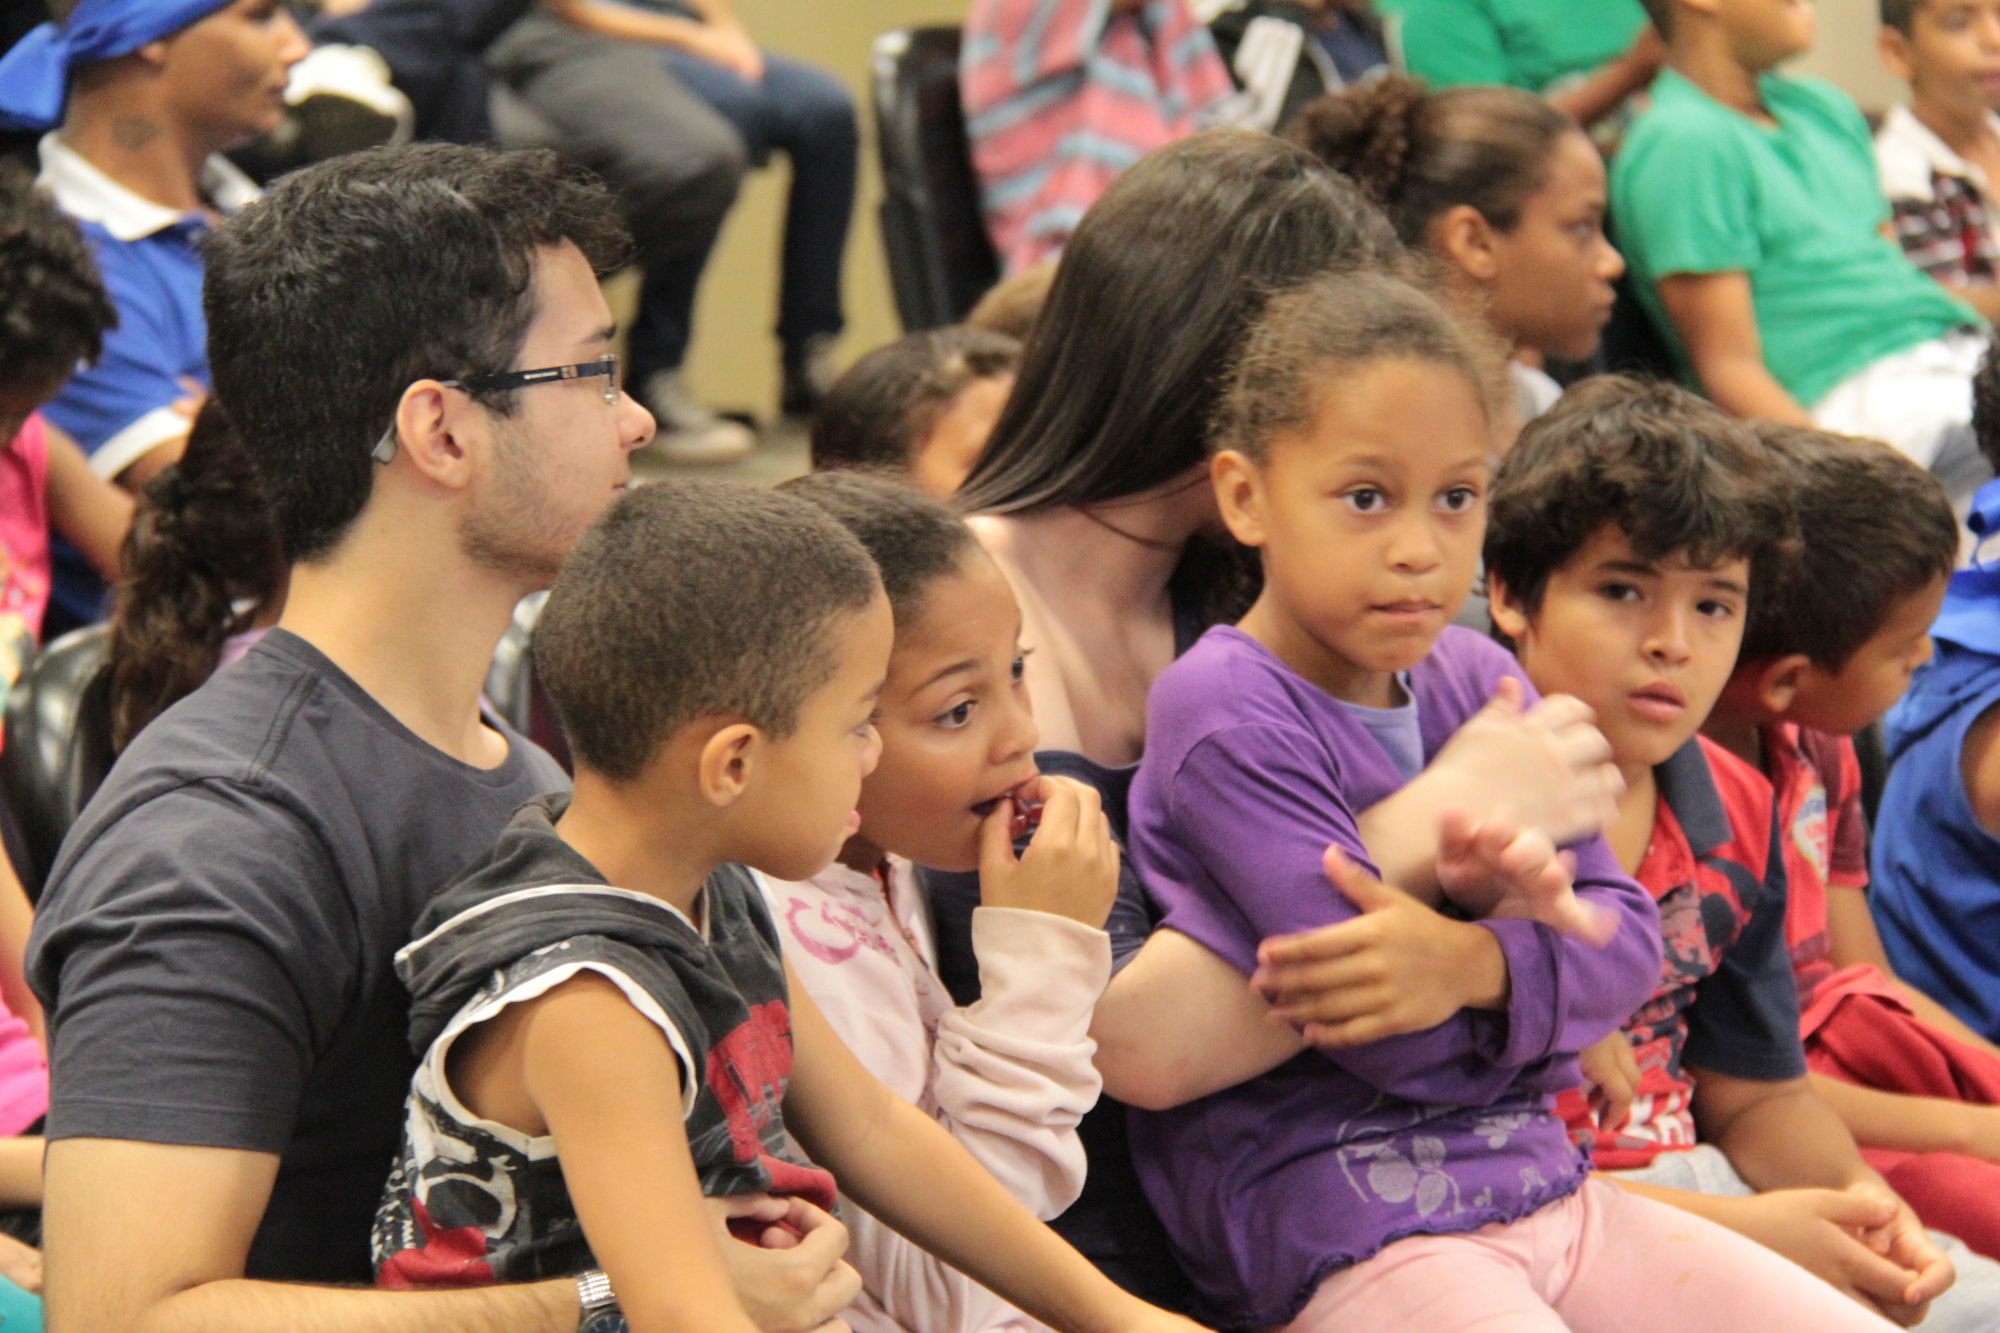
\includegraphics[width=1.0\linewidth]{../../../imagens/dia-das-criancas-2022-10-03-menor.JPG}
                \caption{Evento de comemoração do dia das crianças, com atividades musicais e culturais. Os registros da plataforma apontam para 9 participantes, mas os registros fotográficos indicam uma presença muito maior. (acervo da autora)}
                \label{31e991b69f3aba382518bb571a4e69a720fa8ccb}
\end{minipage}
\hspace{0.5cm}
\begin{minipage}[b]{0.4\linewidth}
        \centering
                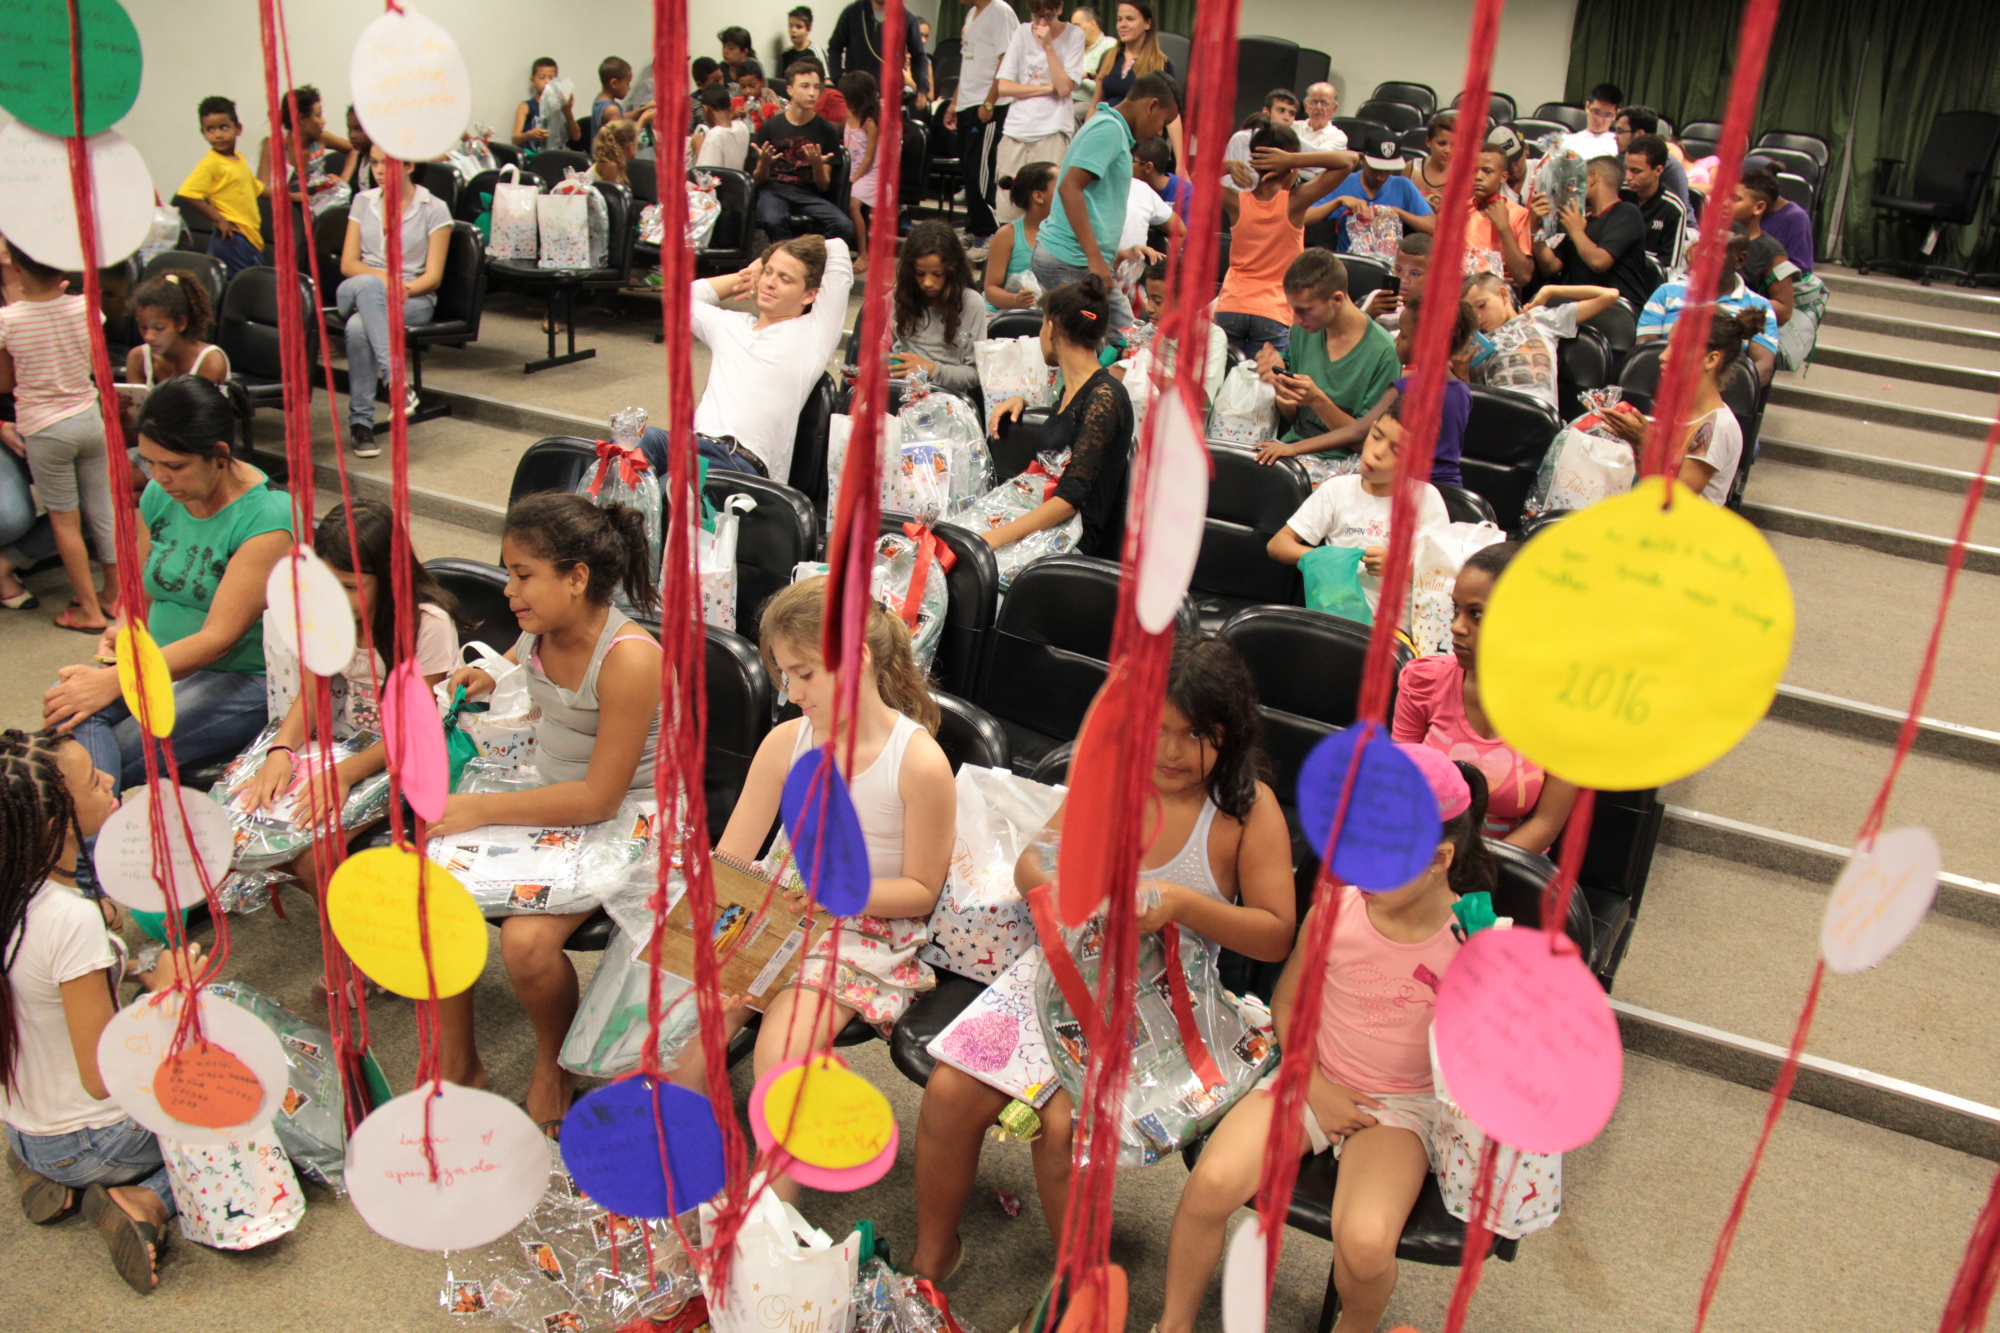
\includegraphics[width=1.0\linewidth]{../../../imagens/confraternizacao-de-natal-menor.jpeg}
                \caption{Evento de Natal realizado no CTI Renato Archer, em 19 de dezembro de 2015. O evento incluiu uma variada gama de atividades lúdicas e educacionais. Muito embora o registro oficial indique a participação de oito pessoas, as fotos mostram que a participação foi muito superior. (acervo da autora)}
                \label{afa1b2acd7f4c590f25d9821e48e82568bd28cf2}
\end{minipage}%
\hspace{0.5cm}
\begin{minipage}[b]{0.4\linewidth}
        \centering
                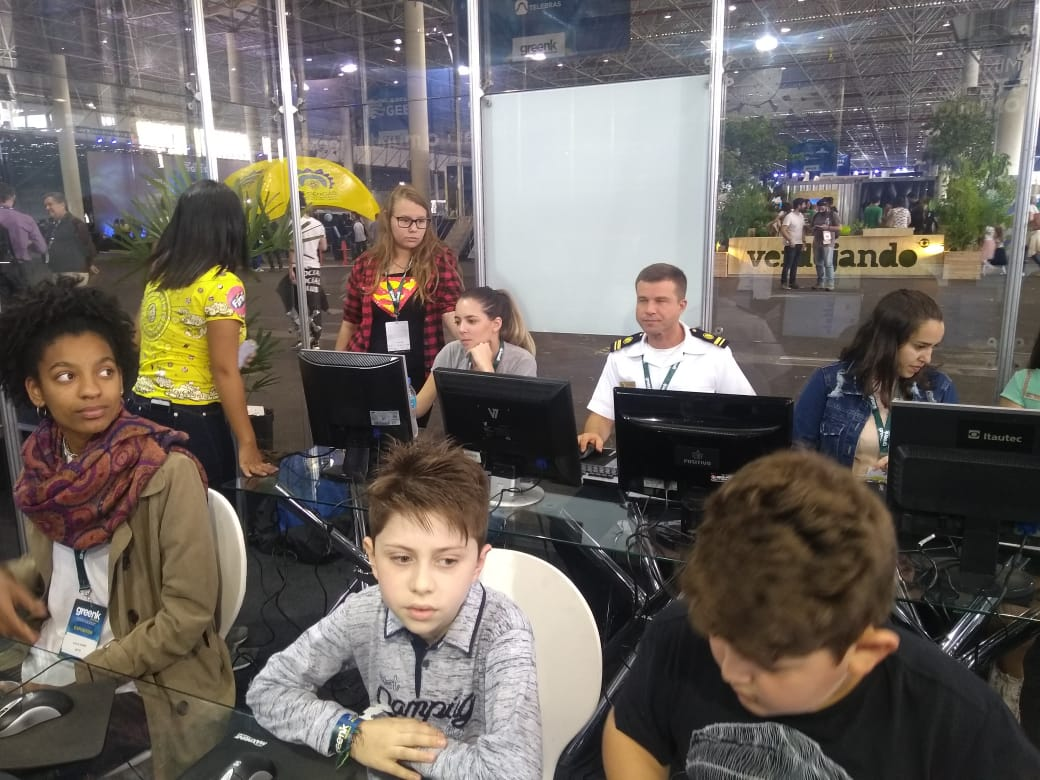
\includegraphics[width=1.0\linewidth]{../../../imagens/Evento-Greenk-2018-05-27.jpg}
                \caption{Evento Greenk, patrocinado pelo MCTI, no Expo Center Anhembi em 27 de maio de 2018, que contou com oficinas do WASH. Neste tipo de evento, é difícil realizar o cadastro nominal de participantes pela amplitude do mesmo. O público beneficiado pode ser estimado em algumas centenas de crianças. (acervo da autora).}
                \label{04766cbd557212dbb84969d429be542b364bf87a}
\end{minipage}
\hspace{0.5cm}
\begin{minipage}[b]{0.4\linewidth}
        \centering
                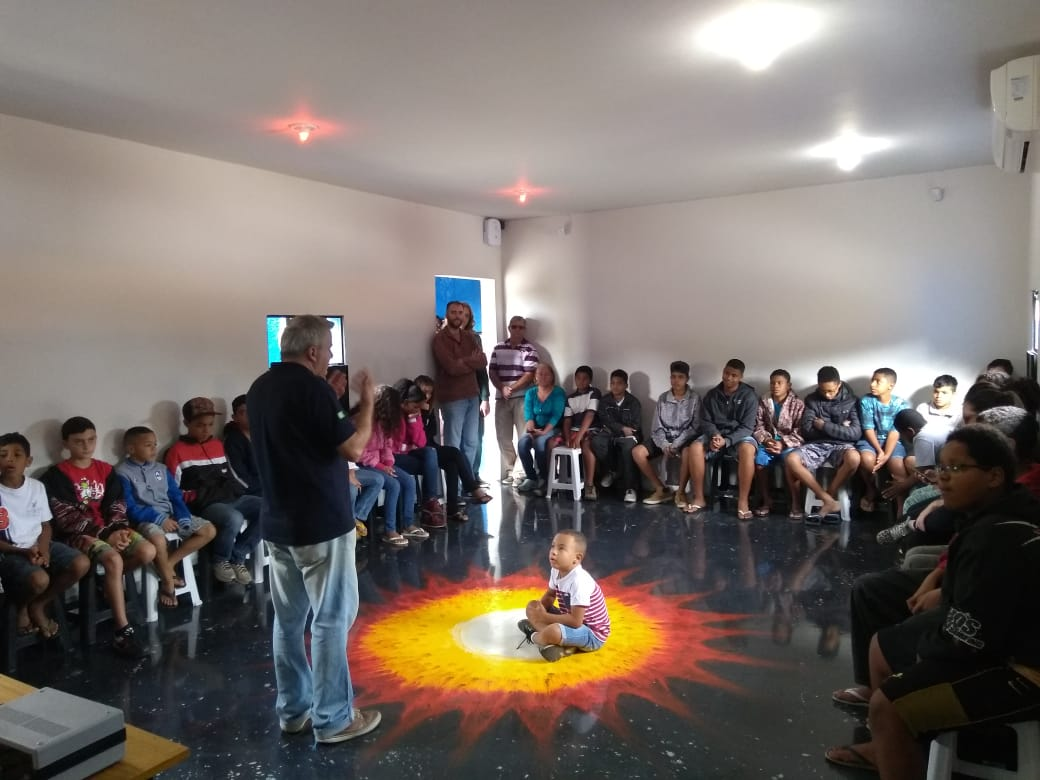
\includegraphics[width=1.0\linewidth]{../../../imagens/MAAS.jpg}
                \caption{Evento no Museu Aberto de Astronomia, promovido pelo WASH. Os registros oficiais não indicam o número de participantes, mas os registros fotográficos mostram a participação de dezenas de crianças. (acervo da autora)}
                \label{b5542509570e0bcdbabe4949f7fef484141b805e}
\end{minipage}%
\hspace{0.5cm}
\begin{minipage}[b]{0.4\linewidth}
        \centering
                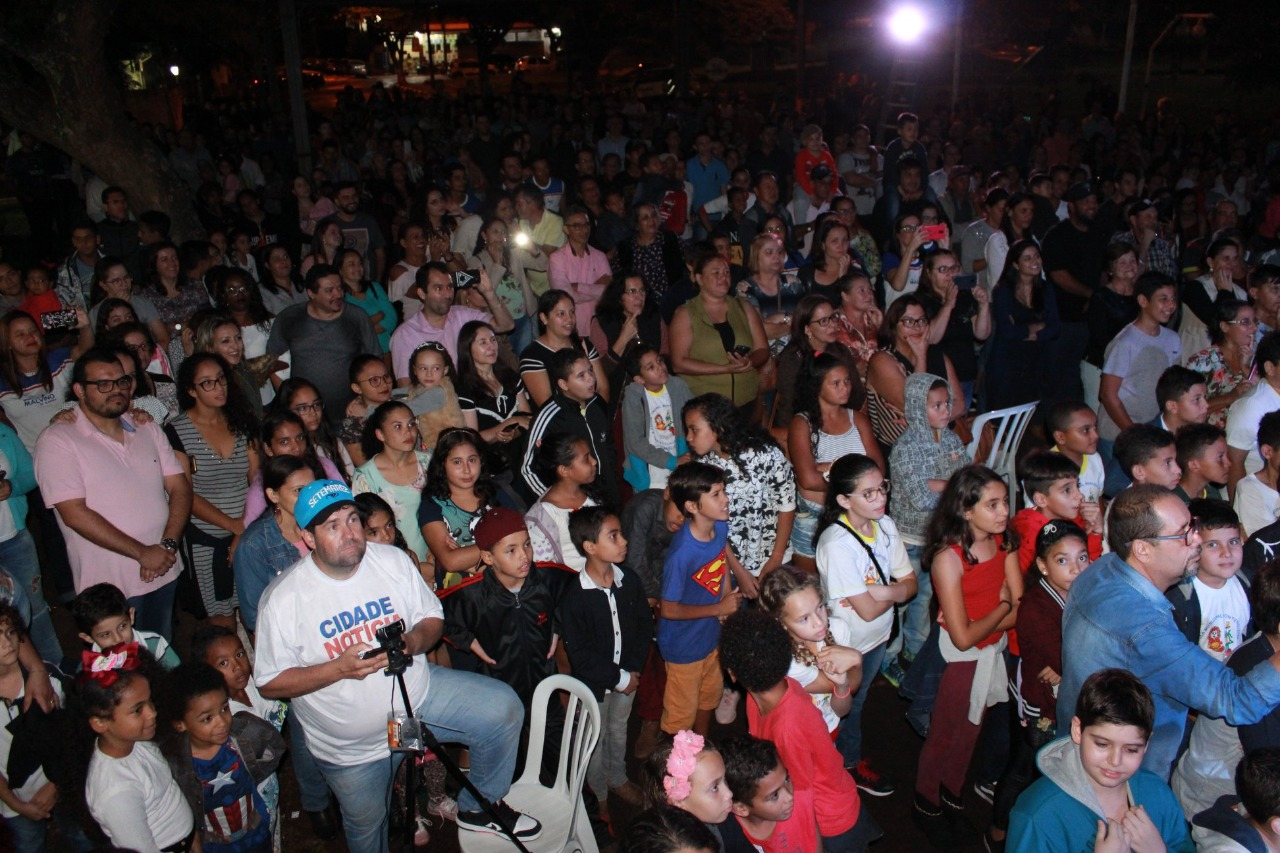
\includegraphics[width=1.0\linewidth]{../../../imagens/Ciencia-Prado-publico.jpeg}
                \caption{Evento de demonstrações científicas, na praça de Prado Ferreira, ocorrido em 31 de maio de 2019, onde o WASH realizou dezenas de oficinas. O evento foi promovido pelo WASH no lançamento do Programa Profissão 4.0 e contou com a participação do Ciência em Show, trupe de artistas formados em física com grande presença na mídia televisiva. (acervo da autora)}
                \label{7b56c85cc265fcbf261a3bc788ae1e4619b70725}
\end{minipage}
\hspace{0.5cm}
\end{figure}







\captionsetup{format=plain}
\begin{figure}[p]

\centering


\begin{minipage}[b]{0.4\linewidth}
        \centering
                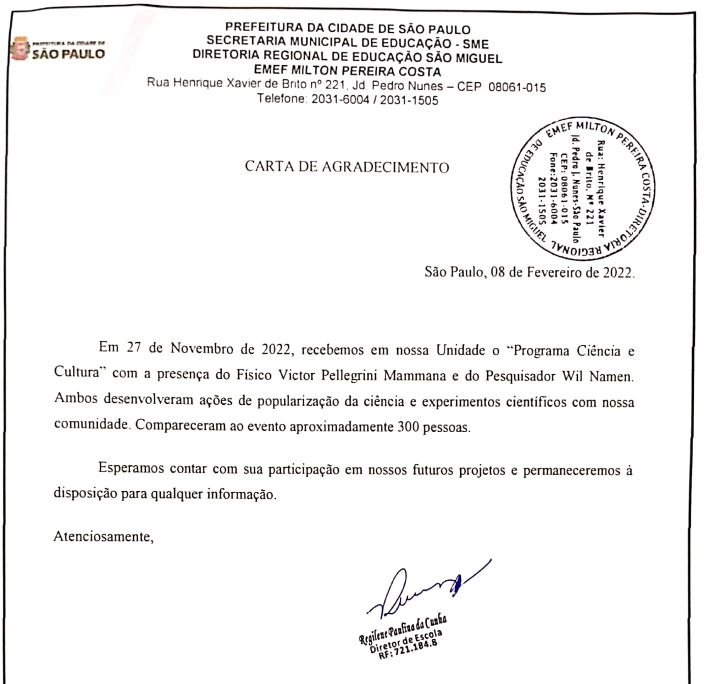
\includegraphics[width=1.0\linewidth]{../../../imagens/evento-sao-miguel.png}
                \caption{Público no evento do Ciência em Show (acervo do Prof. Felipe Cané)}
                \label{1005d976e3ba4fdcea3be1ed7501eff18485a145}
\end{minipage}%
\hspace{0.5cm}
\end{figure}



Com os exemplos de eventos até aqui apresentados, buscamos sustentar a afirmação de que os 3.265 cadastros de participantes representa uma amostra modesta de todos os beneficiários do Programa WASH. Outra evidência que sustenta essa informação é o número de 3.771 eventos realizados, segundo os registros do Recorte B (ver seção 3.2). Muito embora ocorra a retenção de público, com participantes de mais de um evento, a existência de mais eventos do que participantes recomenda um cuidado maior com a possibilidade de o número de pessoas beneficiárias estar subestimado.

Não obstante esse caráter amostral, ou seja, incompleto em termos de registros individuais dos participantes, sustentamos que essa amostra é adequada para extrair importantes informações sobre o Programa. Entre elas está o seu crescimento anual, o impacto da pandemia e o perfil etário do público alvo, por exemplo, o que pode ser verificado nas seções a seguir.

\subsection[Evolução temporal do número de participações]{Evolução temporal do número de participações}\label{Evolução temporal do número de participações}
Mesmo não representando o universo completo de participantes, os dados amostrais são importantes para identificar tendências do Programa, a exemplo da evolução anual do número de participações, mostrada na Fig. 37.



\captionsetup{format=plain}
\begin{figure}[p]

\centering


\begin{minipage}[b]{0.4\linewidth}
        \centering
                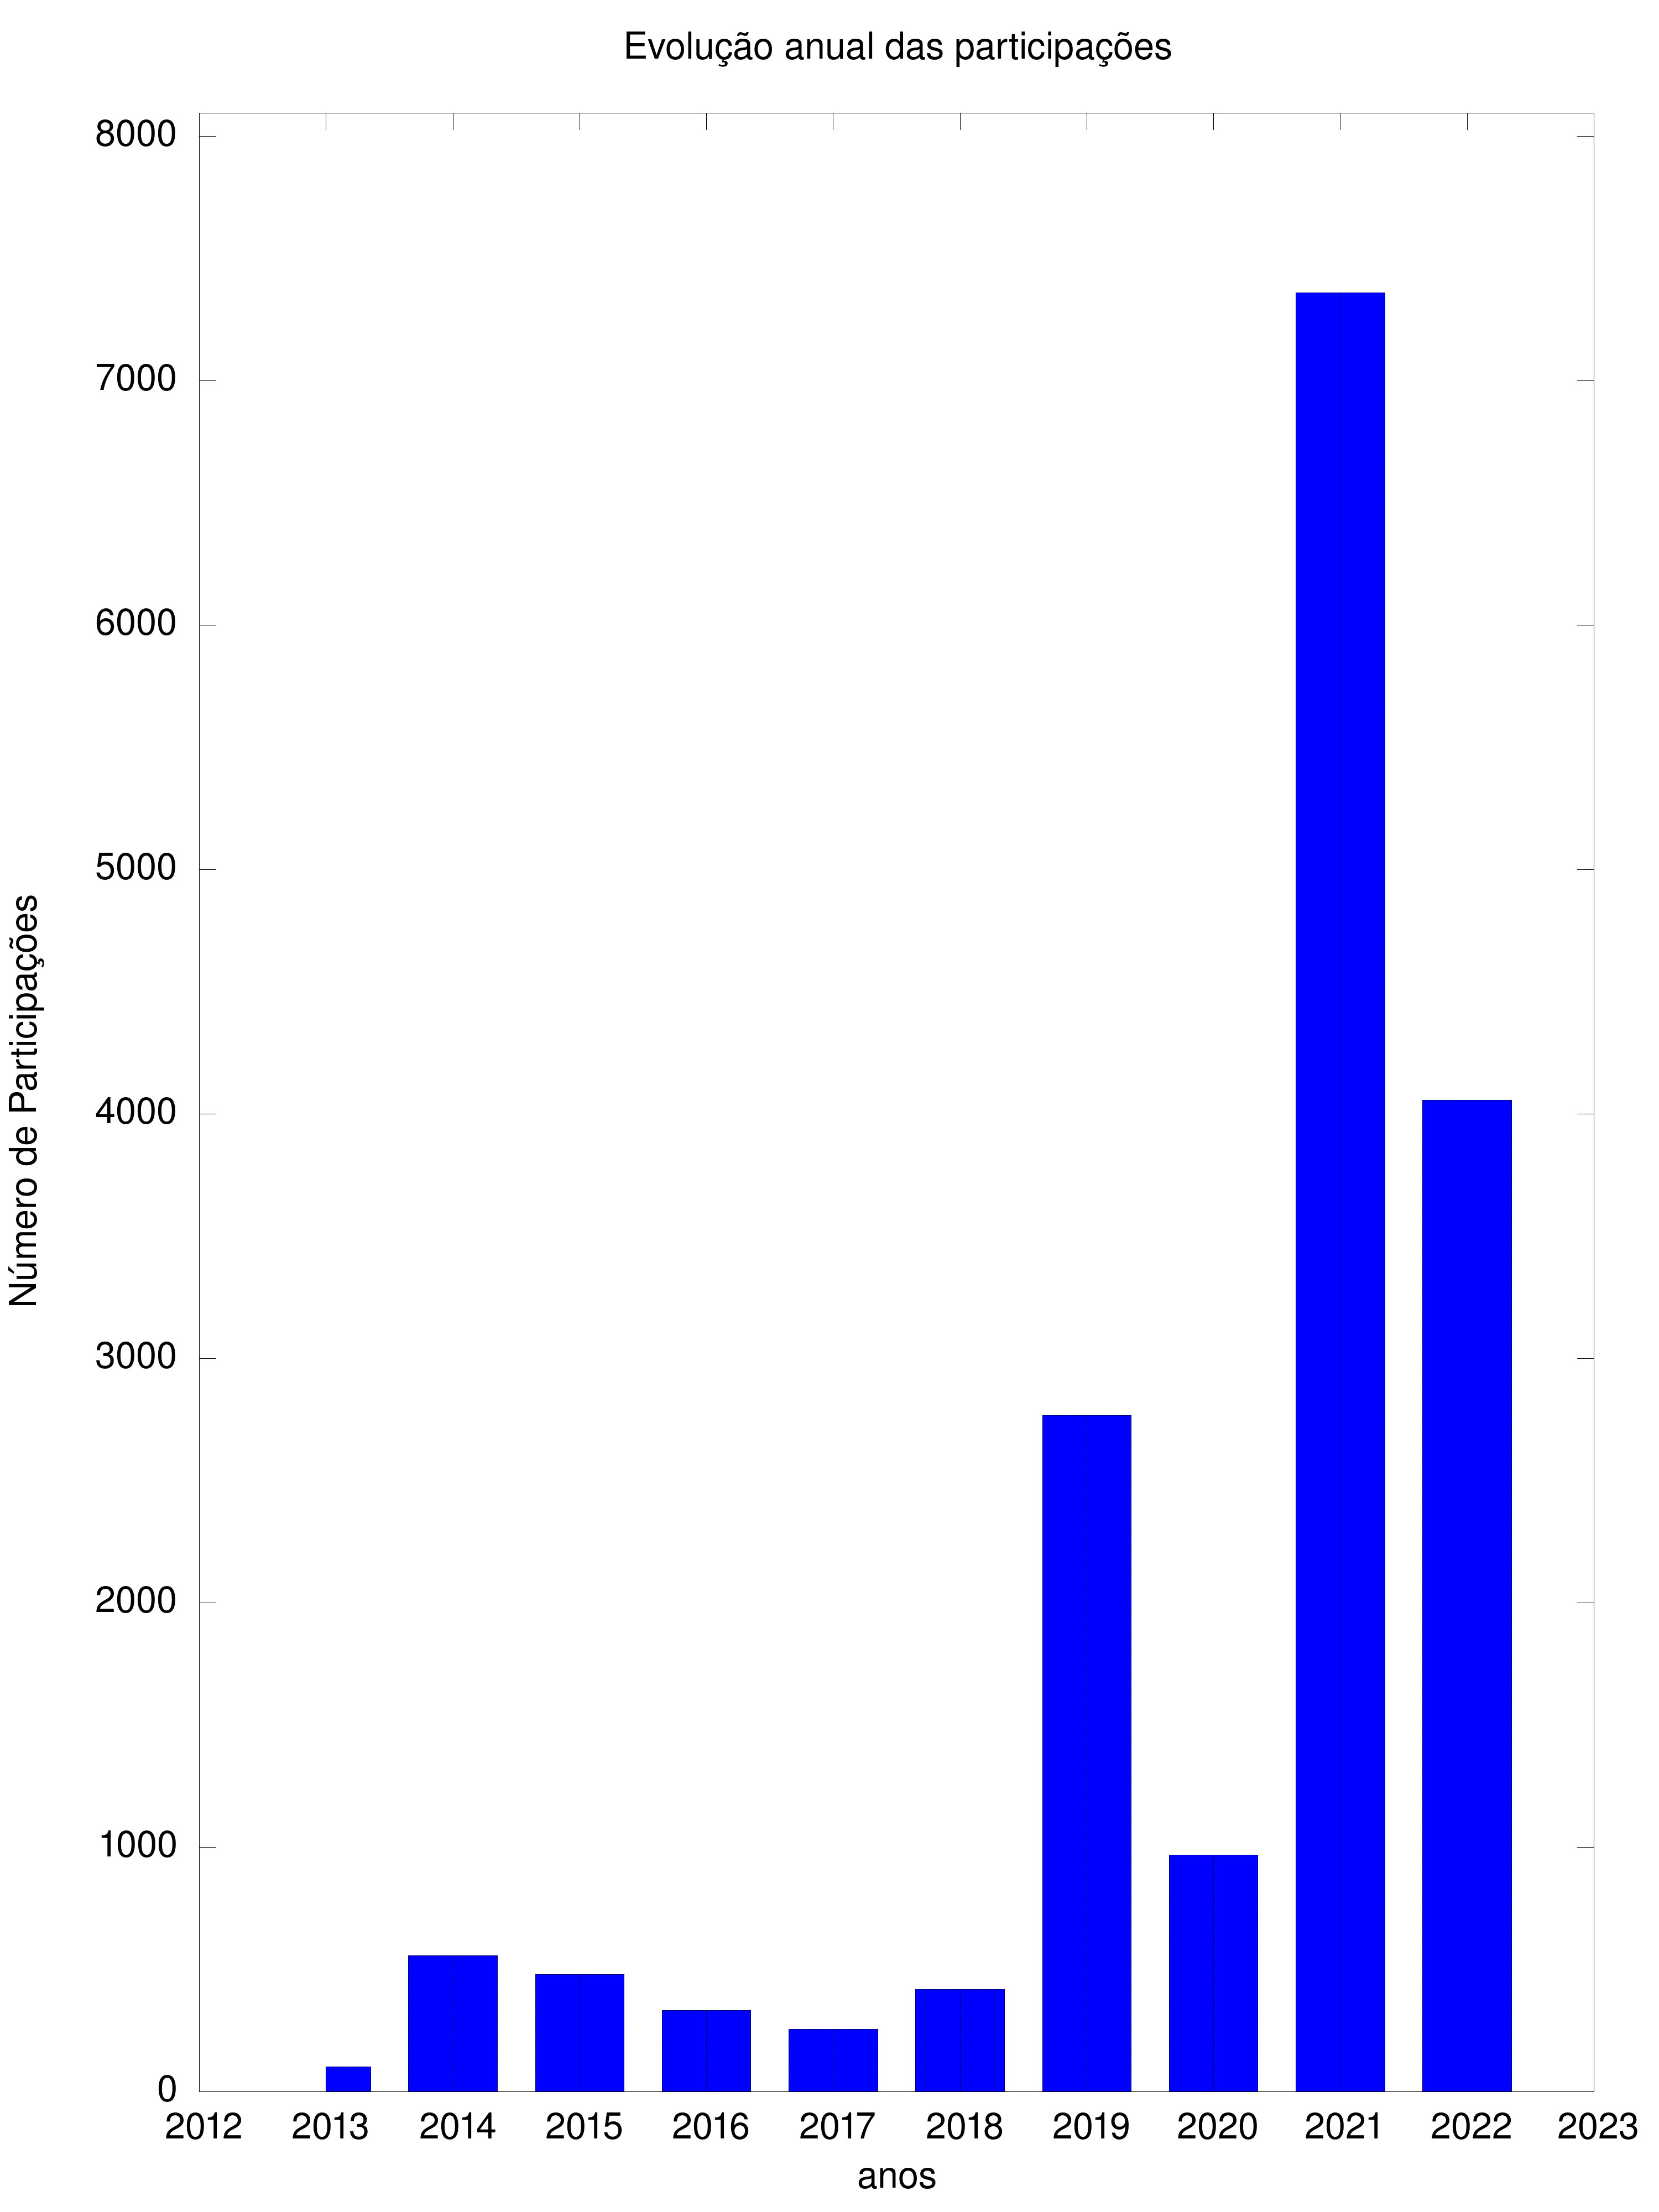
\includegraphics[width=1.0\linewidth]{../../../imagens/output-participantes.jpeg}
                \caption{Evolução temporal do número de participações ao longo dos 10 anos de existência do Programa WASH, segundo o Recorte A (fonte: elaboração própria).}
                \label{19699bcc5ab8317274249d6743d62534dbfb95fa}
\end{minipage}%
\hspace{0.5cm}
\begin{minipage}[b]{0.4\linewidth}
        \centering
                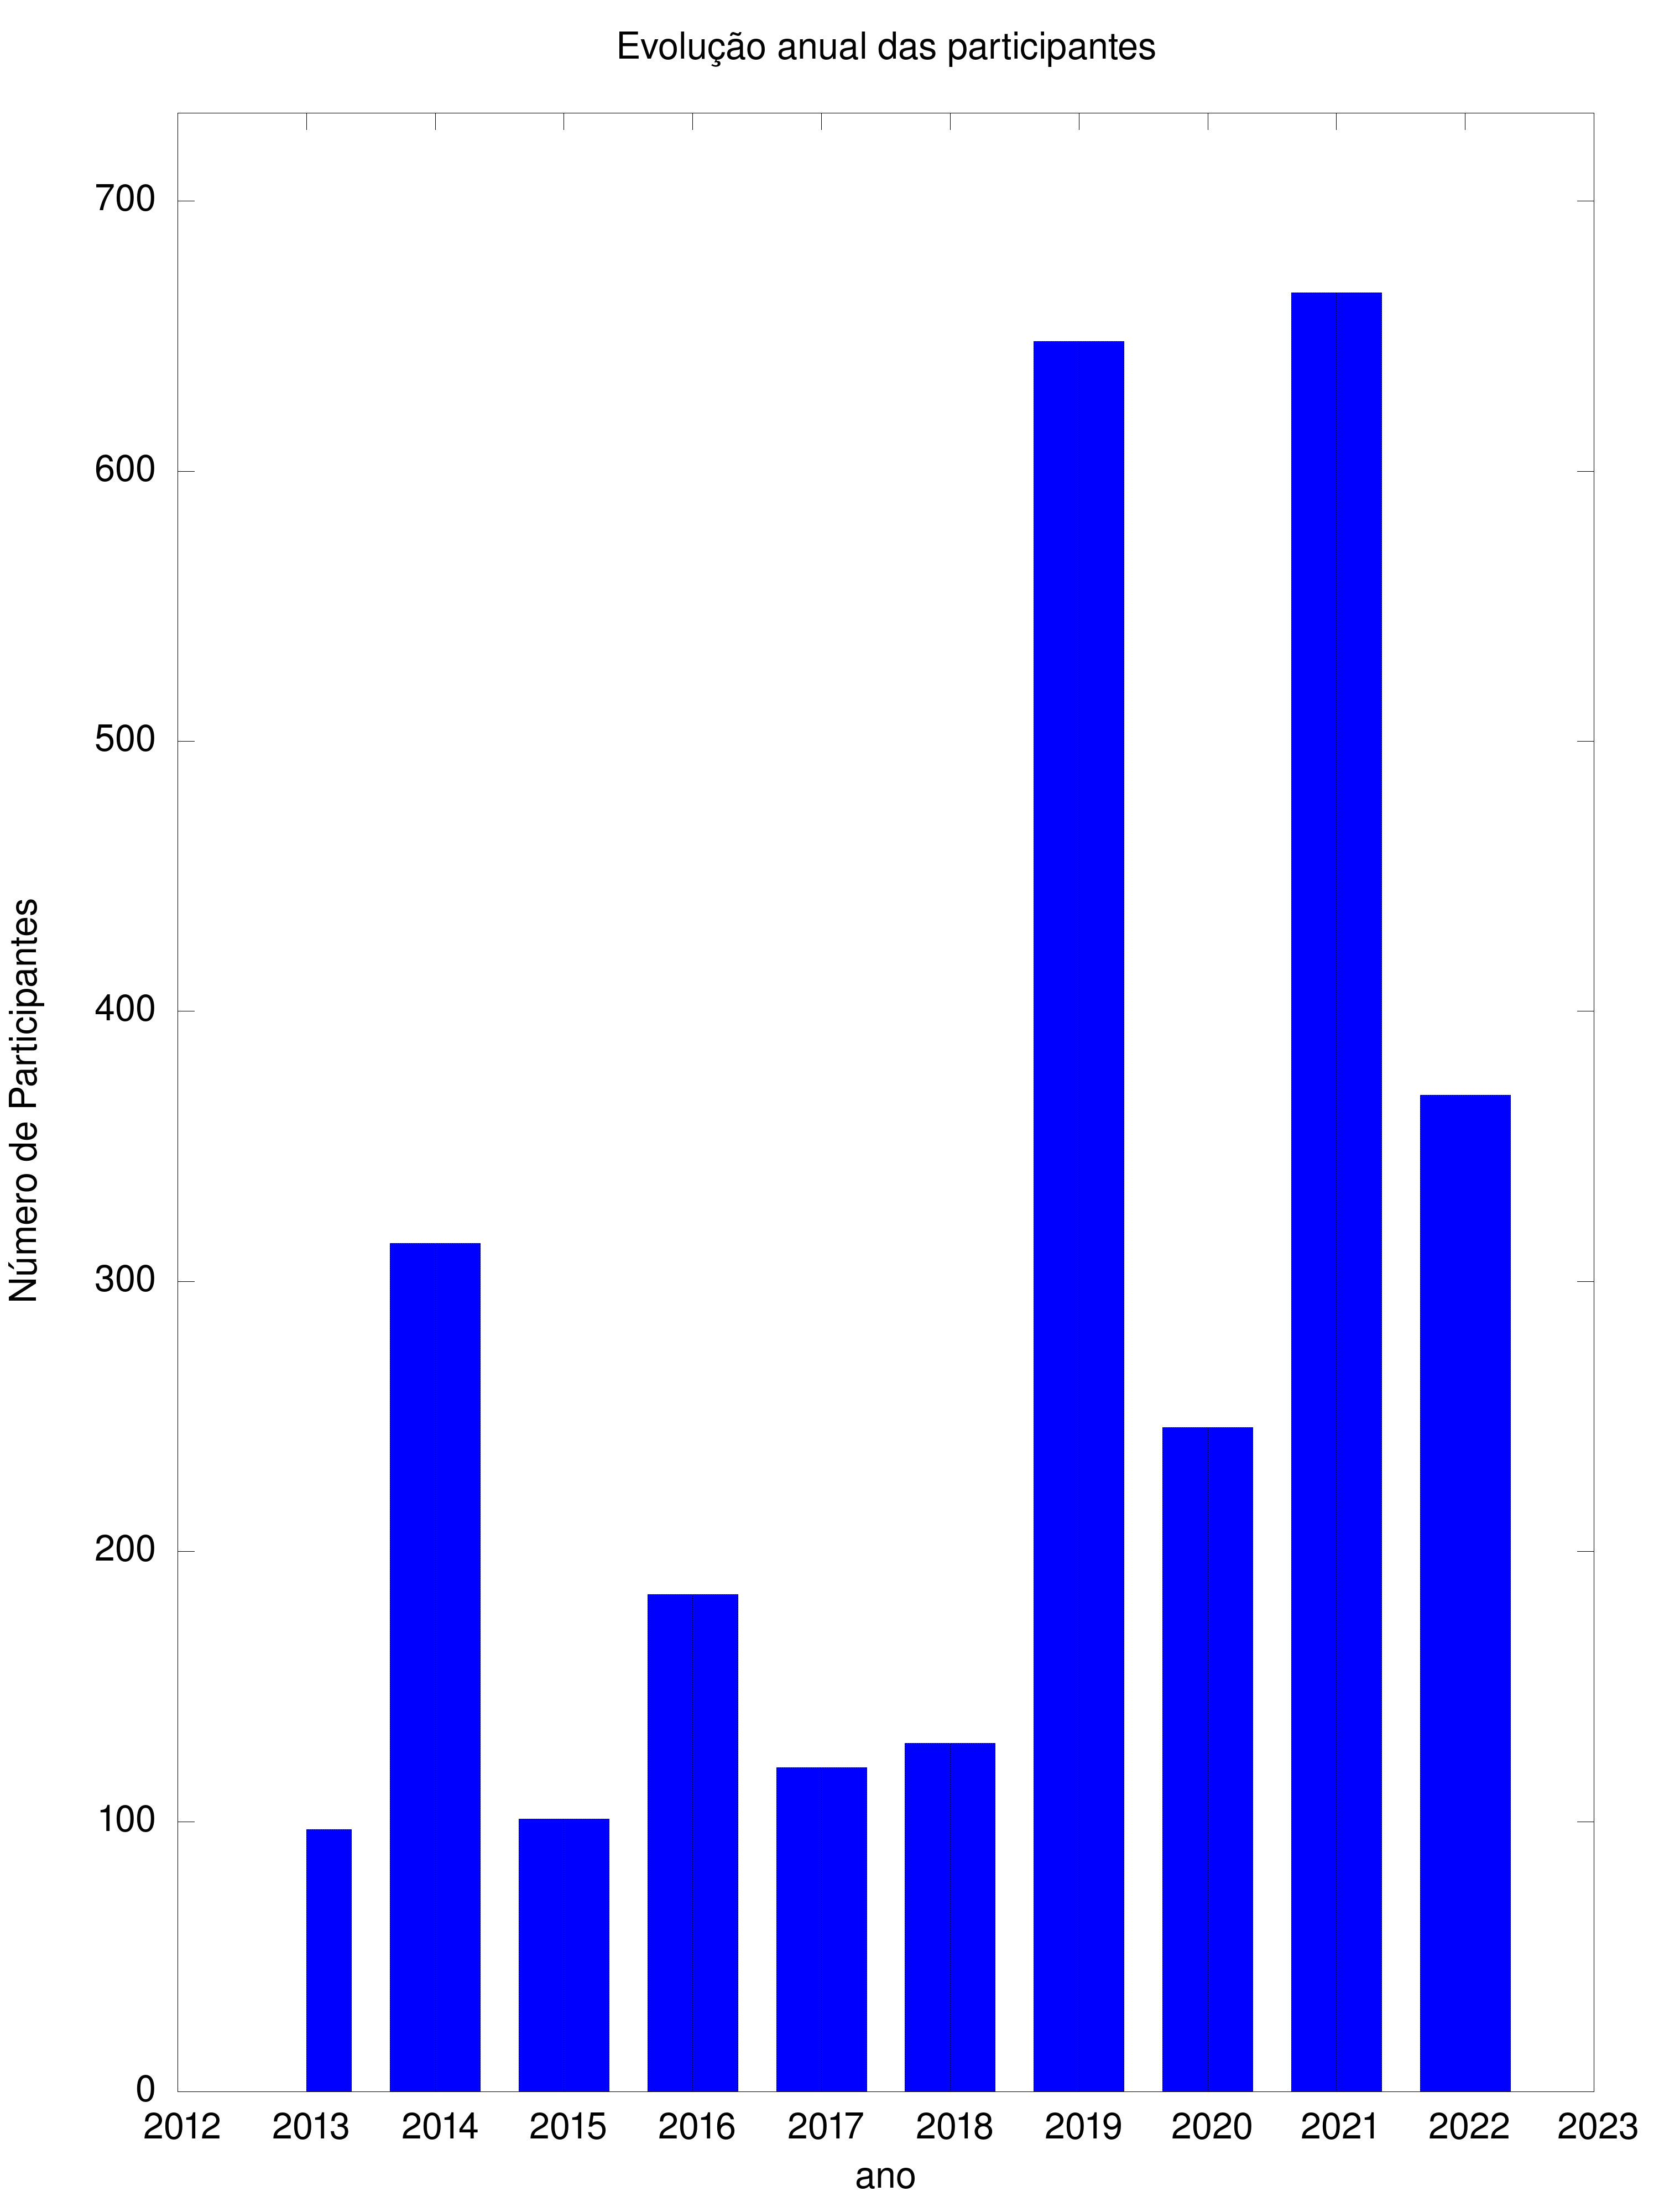
\includegraphics[width=1.0\linewidth]{../../../imagens/output-participantes2.jpeg}
                \caption{Evolução anual do número de participantes individuais segundo o Recorte A (fonte: elaboração própria).}
                \label{e01eb26f443a577db4a1d382417f8c1bb57ee435}
\end{minipage}
\hspace{0.5cm}
\begin{minipage}[b]{0.4\linewidth}
        \centering
                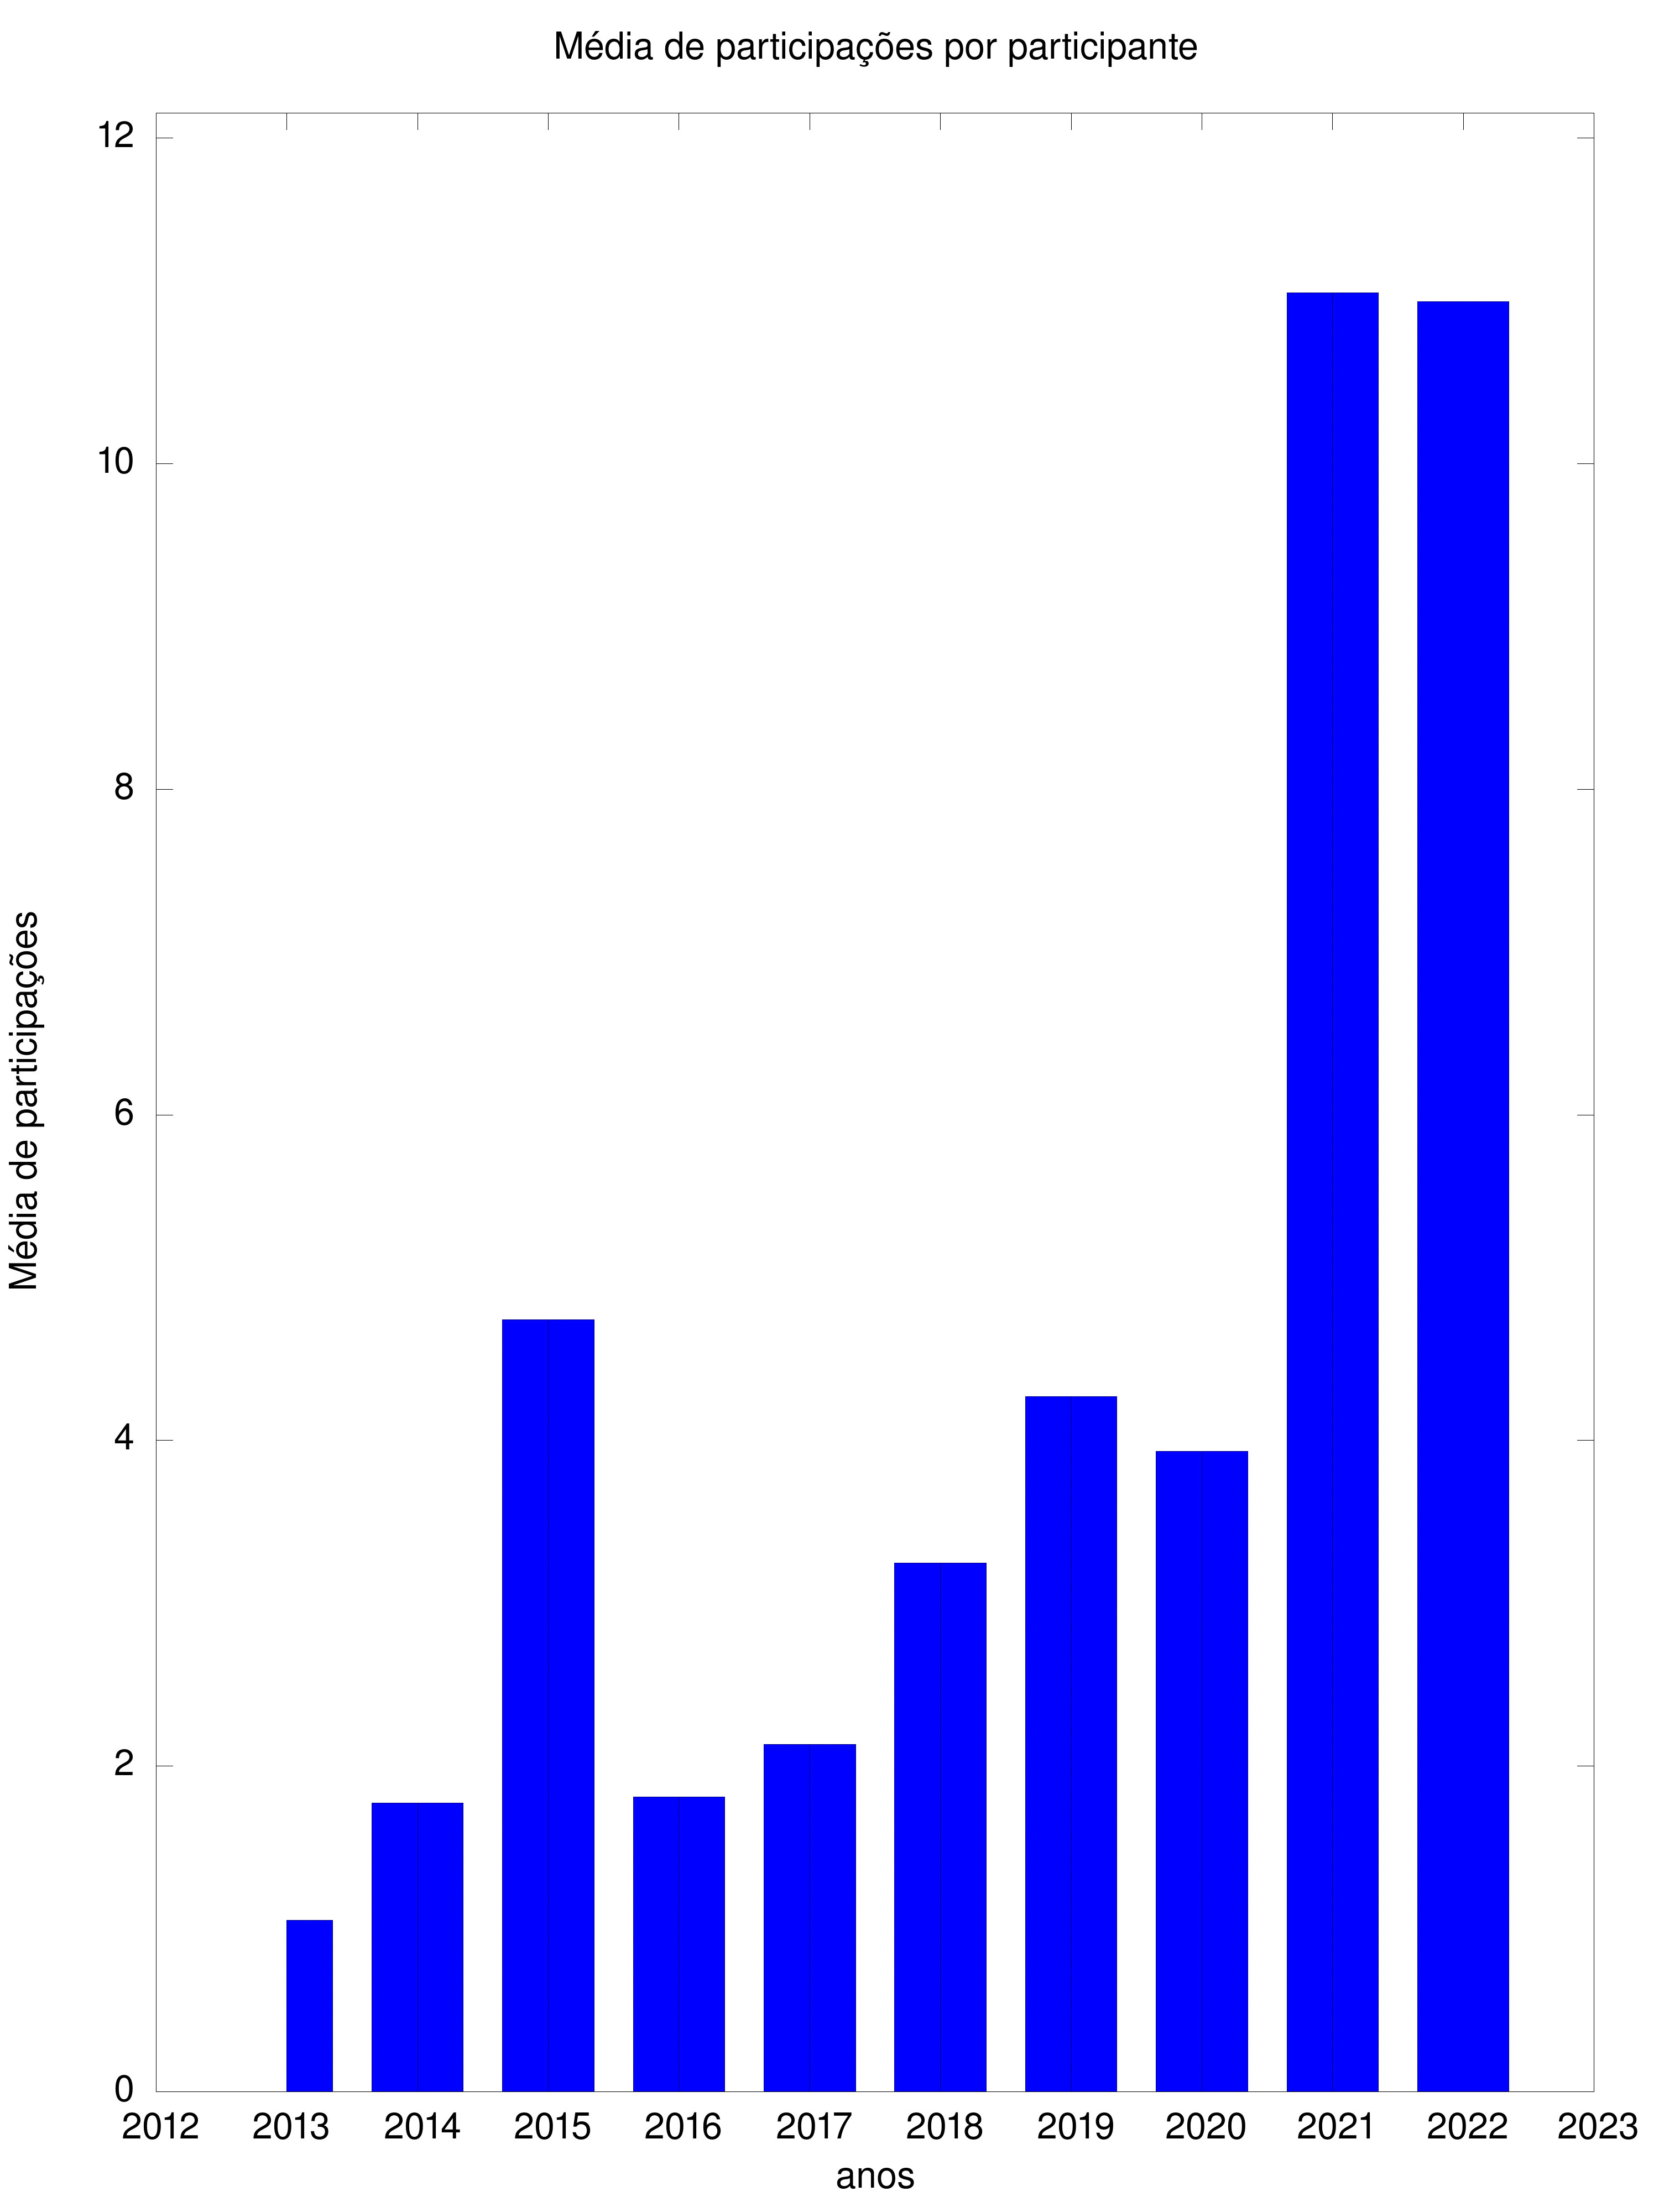
\includegraphics[width=1.0\linewidth]{../../../imagens/output-media-participacoes.jpeg}
                \caption{Evolução anual da média de participações por participante segundo, o Recorte A (fonte: elaboração própria).}
                \label{a8f2d72073b88290f9b8731b144383d2f7c4dc4b}
\end{minipage}%
\hspace{0.5cm}
\end{figure}



É importante atentar para uma sutileza: a diferença entre o " número de participantes" e o "número de participações".

O número de participações, mostrado na Fig. 37, significa o número de vezes que participantes frequentaram eventos do WASH naquele ano, ainda que seja contabilizada a mesma pessoa duas ou mais vezes.

O número de participantes, mostrado na Fig. 38, significa o número de indivíduos que partiparam de eventos naquele ano, contabilizados uma vez só, ainda que tenham participado em mais de um evento no mesmo ano.

A Fig. 39 mostra a média de participações por participante, dividindo, um a um, os dados da evolução anual das participações pela evolução anual dos participantes. Como se vê no gráfico, os dados amostrais indicam um crescimento no número de "retornos" de participantes.

Os gráficos de evolução anual de participações (ver Fig. 37), participantes (ver Fig. 38) e de média de participações (ver Fig. 39) indicam um crescimento do Programa WASH, principalmente a partir de 2019, ano em que houve também um crescimento no número de emendas parlamentares.

Ao mesmo tempo, os gráficos indicam que a pandemia teve impacto negativo no atendimento de educandos por parte do WASH, uma vez que observou-se uma queda abrupta em 2020, tanto em termos de participações quanto de participantes.

Não obstante a manutenção de parte das restrições de isolamento social no ano de 2021, os gráficos das Figs. 37 e 38 mostram uma recuperação nos indicadores de participantes e participações naquele ano (lembrando que os dados para 2022, no Recorte A, são parciais). Atribuímos essa recuperação às medidas tomadas pelo WASH de desenvolver oficinas remotas, mesmo o WASH ter sido concebido como Programa presencial  (CTI, 2018). Essas medidas estão descritas na seção 4.1.6.

Esse aprendizado sobre como realizar oficinas remotas precisa se refletir na revisão do Documento de Referência do WASH, uma vez que o anexo à Portaria CTI 178/2018 não traz qualquer referência a este método.

Finalmente, é preciso enfatizar que os dados para 2022 são parciais, uma vez que a presente análise refere-se a um Recorte A, cujo período se encerra em agosto daquele ano.

\subsection[Distribuição de partipantes por sexo (equidade)]{Distribuição de partipantes por sexo (equidade)}\label{Distribuição de partipantes por sexo (equidade)}
As pessoas do sexo feminino são particularmente desprivilegiadas quando o tema é igualdade de acesso às disciplinas de Science, Technology, Engineering and Mathematics (Kijima et al.,2021).

Por esta razão, é de muito interesse para este trabalho analisar o equilíbrio no atendimento a participantes do sexo masculino e do sexo feminino, com vistas a determinar a equidade.

Mas esta análise, como antecipado no capítulo de Materiais e Métodos, não foi planejada no início do Programa.

Portanto, identificamos a necessidade de desenvolver um método para estimar o equilíbrio entre participantes femininos e masculinos, criando um indicador de equidade. Este método é baseado na contagem dos registros, cujo o primeiro nome do cadastrado está presente numa lista de "nomes masculinos"; e na contagem simultânea dos registros, cujo o primeiro nome da cadastrada está presente numa lista de " nomes femininos" (ver detalhes em Materiais e Métodos, seção 3.2.4).

Este método de " estimativa " não tem a finalidade de atribuir, individualmente, o sexo a cada participante porque não se deseja estigmatizar os participantes que, por falha de cadastro do Programa, não tiveram a oportunidade de fazer sua autodeclaração de sexo.

A partir de 2019, foi incluído na plataforma Platuóxe um campo autodeclaratório sobre sexo do (a) participante, uma parte dos dados usada para gerar o indicador de equidade foi fornecida pelos (as) próprios (as) participantes.

O gráfico abaixo mostra a distribuição dos sexos feminino, masculino,  desconhecido e outros, no universo de participantes do WASH. Nota-se um equilíbrio entre o número de participantes, sendo 49.4\%  mulheres e 48.3\% homens, havendo ainda 2.1\% de sexo desconhecido. Apenas cinco cadastros apontam a identidade de gênero autodeclarada.

O gráfico de "pizza" da Fig. 44 mostra a distribuição de participantes do sexo masculino e feminino, referindo-se ao universo de participantes cadastrados na Platuóxe, de acordo com Recorte A, independentemente do tipo de vínculo. Uma outra informação importante para avaliar a equidade do Programa  WASH é a que foi levantada por (FINK (2022), para o período de 2020 a 2021, período no qual foi possível identificar uma significativa prevalência de bolsistas do sexo masculino, como indicado na Fig. 41, para uma amostra de 101 bolsistas. Essa amostra refere-se a uma única emenda (Processo CNPq 4000172015-6). Um estudo mais amplo de distribuição de bolsas por sexo precisa ser realizado para avaliar se essa tendência continua presente. Do ponto de vista desta dissertação, essa situação norteou a revisão do Documento de Referência, como se verá na seção 7.2.



\captionsetup{format=plain}
\begin{figure}[p]

\centering


\begin{minipage}[b]{0.4\linewidth}
        \centering
                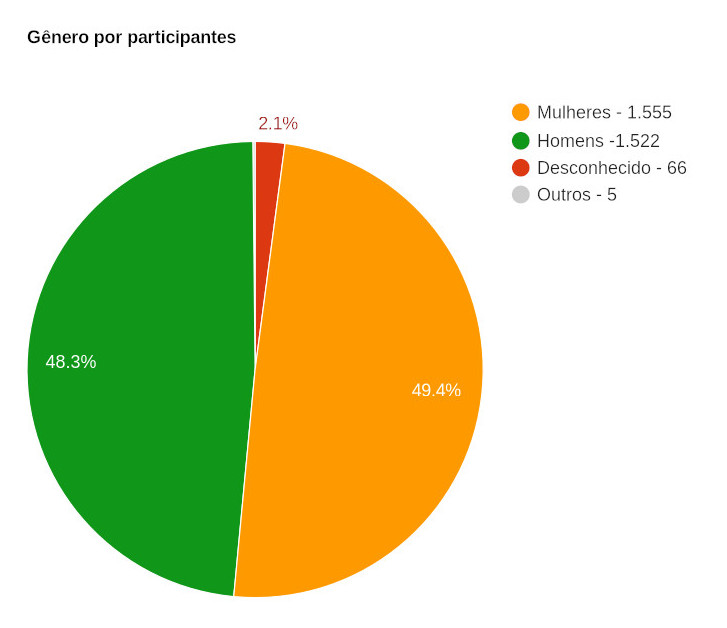
\includegraphics[width=1.0\linewidth]{../../../imagens/genero-todos-crop.jpeg}
                \caption{Distribuição dos participantes por sexo. Esses dados foram obtidos por meio de inferência, a posteriori, utilizando o primeiro nome dos participantes como forma de estimar o percentual de participantes de ambos os sexos. (fonte: elaboração própria)}
                \label{ef11d820efb73d78fb64eb6bdd03853471a8e89f}
\end{minipage}%
\hspace{0.5cm}
\begin{minipage}[b]{0.4\linewidth}
        \centering
                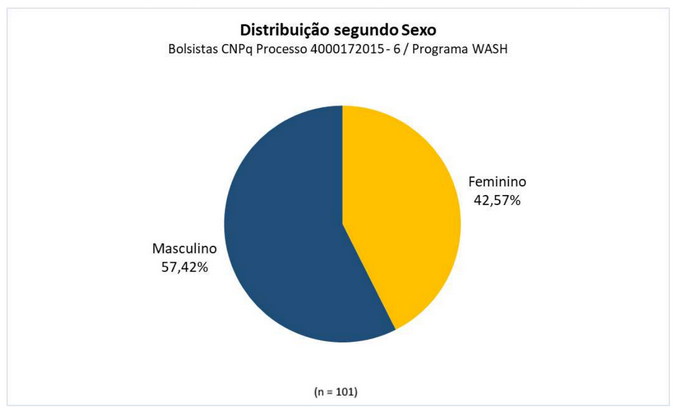
\includegraphics[width=1.0\linewidth]{../../../imagens/distribuicao-sexo-bolsistas.png}
                \caption{Distribuição de bolsistas por sexo, indicando prevalência de bolsistas do sexo masculino para a emenda referente ao Processo CNPq 4000172015-6. O período de análise foi de 2019 a 2020. (fonte: [[FINK (2022)]])}
                \label{1164a3115bd14e3f25b6b141840652ffbd0d2374}
\end{minipage}
\hspace{0.5cm}
\end{figure}



\subsection[Número de Bolsistas]{Número de Bolsistas}\label{Número de Bolsistas}
O método do WASH pressupõe a atuação de bolsistas de iniciação científica, extensão e apoio tecnológico nas seguintes modalidades: ITI A, ITI B, EXP, ATP e ADC, conforme política de Bolsas do CNPq. Os bolsistas realizam suas pesquisas previstas em plano de trabalho, devendo, também, atuar como multiplicadores do Programa.

Para determinar o número de bolsistas no Programa WASH, decidimos utilizar o Recorte B, aplicando consultas estruturadas, de caráter mais genérico, na Platuóxe, trabalho desenvolvido por Michel Alencar Morandi e publicadas em (WASH, 2023).

Para averiguar a abrangência dos dados sobre os (as) bolsistas, no Recorte B da Platuóxe, apresentamos a evolução anual de concessão de bolsas, mostrada na Fig. 42.



\captionsetup{format=plain}
\begin{figure}[htb]

	\begin{center}

		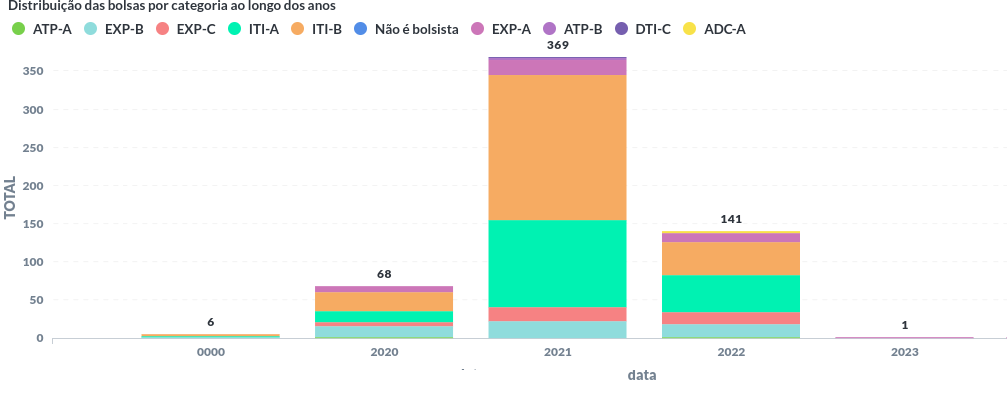
\includegraphics[max size={\textwidth}{\textheight}]{../../../imagens/bolsas-anualmente-recorte-b-crop.png}

	\end{center}

	\caption{\label{3f695a85b367790579065c12b40bfa0acdd593f2}Evolução anual de bolsistas do WASH, segundo o Recorte B. As cores indicam modalidades de bolsas. (fonte:  [[WASH (2023)]], por demanda da autora)}

\end{figure}

A Fig. 42, por não apresentar dados para anos anteriores a 2020, mostra que os dados de bolsistas, presentes no Recorte B da Platuóxe não refletem a totalidade de bolsistas do Programa, mesmo que o Recorte B se refira a um período iniciado em setembro de 2013. Em outras palavras, a Fig. 42 mostra que na Platuóxe estão registradas apenas bolsas iniciadas  em 2020, 2021 e 2022. Isso ocorre porque o armazenamento dos dados de bolsistas não fazia parte da versão original da Platuósh, que passou a ter esse recurso apenas a partir de 2019-2020. A barra com legenda "0000" indica que há dados espúrios na amostra, os quais devem ser desconsiderados ("0000" indica que o ano de concessão da bolsa registrada na Platuóxe é desconhecido).

A interpretação do gráfico da Fig. 42 requer um cuidado: ele não mostra as bolsas vigentes, mas iniciadas em determinado ano. Portanto, a barra para o ano de 2022, por exemplo, pode dar a ideia errônea de que houve uma redução de bolsistas naquele ano, mas, a rigor, há bolsas iniciadas em 2021 que ainda podem estar vigentes em 2022. Nesse caso, o número de bolsistas vigentes em 2022 seria maior do que o número de bolsas iniciadas em 2022.

Apesar da limitação do Recorte B que traz dados de bolsistas limitados aos anos de 2020 a 2023, ainda assim é possível desenvolver análises de utilidade para essa dissertação. Mas, não se deve perder de vista que essas análises são de caráter amostral.

A Fig. 43 mostra a distribuição de modalidades de bolsas do WASH, concedidas a partir de 2020 (subconjunto do Recorte B).



\captionsetup{format=plain}
\begin{figure}[htb]

	\begin{center}

		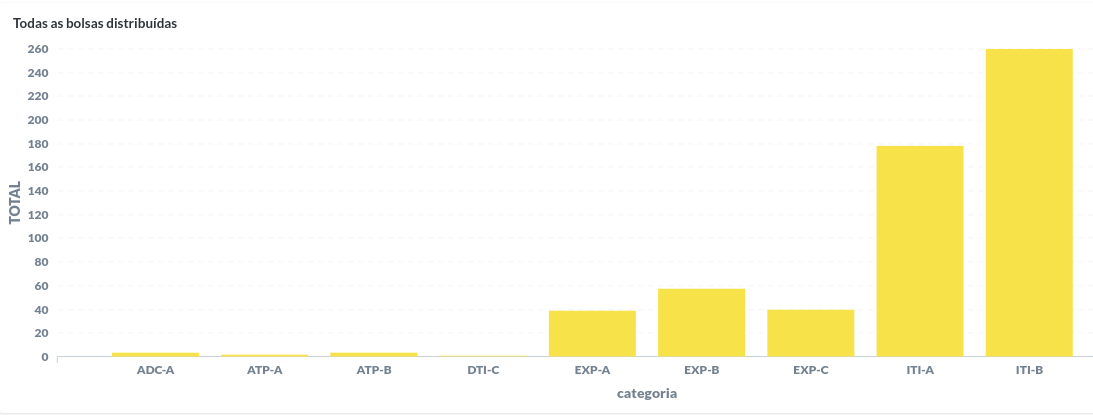
\includegraphics[max size={\textwidth}{\textheight}]{../../../imagens/quantidade-bolsistas-3.png}

	\end{center}

	\caption{\label{27e98d39e299354bc7619996ee91fe3d2cf0e56c}Distribuição de modalidades de bolsas no Programa WASH. (fonte: [[WASH (2023)]], por demanda da autora)}

\end{figure}

Os dados do gráfico da Fig. 43 podem ser vistos na Tabela 11.

A Tabela 11 mostra que 75\% das bolsas do WASH, concedidas entre 2020 e 2023 (Recorte B), são dedicadas para a iniciação científica (ITI A e ITI B). Isso é um indicativo de que o público alvo do Programa, definido pela Portaria CTI 178/2018, tem sido priorizado, dado que são os bolsistas de iniciação científica que desempenham o papel de multiplicação junto aos educandos das redes de ensino e de outras entidades responsáveis. De fato, a Portaria CTI 178/2018 prevê:


\noindent\begin{center}\mbox{\centering\fbox{\centering\par\parbox{0.7\linewidth}{\small\textit{"O público alvo das oficinas deve ser constituído preponderantemente de estudantes do ensino fundamental, mas adolescentes e adultos também podem participar, a exemplo dos pais dos educandos, os quais são sempre convidados." (fonte: Portaria CTI 178/2018).}\normalsize}}}\end{center}






\begin{table}[htb]
\tiny
\caption{\label{ce6a9b067c8c0983df5f5cd1fd18c89955204b38}Distribuição de bolsas por modalidade no Recorte B da Platuóxe, ressalvando que, nesse recorte, há apenas dados das bolsas concedidas a partir de 2020. (fonte:  [[WASH (2023)]], por demanda da autora).}

\centering
\begin{tabular}{|c|c|c|}
\hline
modalidade de Bolsa  &  tipo  &  quantidade \\
\hline
ITI A  &  iniciação  &  178 \\
ITI B  &  iniciação  &  260 \\
EXP A  &  extensão  &  39 \\
EXP B  &  extensão  &  57 \\
EXP C  &  extensão  &  40 \\
ATP A  &  extensão  &  2 \\
ATP B  &  extensão  &  3 \\
ADC A  &  difusão  &  3 \\
DTI C  &  desenvolvimento  &  1 \\
\hline
  &  TOTAL  &  583 \\
\hline
\end{tabular}
\end{table}


Outro aspecto no Recorte B é a prevalência de bolsas de iniciação para estudantes do ensino médio, uma ênfase que está tacitamente presente no Documento de Referência do WASH.


\noindent\begin{center}\mbox{\centering\fbox{\centering\par\parbox{0.7\linewidth}{\small\textit{"Os monitores/bolsistas devem ser estudantes do ensino médio que, como forma de estímulo, recebam bolsas de iniciação científica. Também, são aceitos como monitores/bolsistas os alunos do ensino superior, desde que beneficiados por bolsas de iniciação científica compatíveis." (fonte: Portaria CTI 178/2018)}\normalsize}}}\end{center}


Essa prevalência do ensino médio é diferencial em relação a outros programas de iniciação científica da academia, que focalizam a iniciação científica a partir do ensino superior.

Além das análises pertinentes ao Recorte B, é possível complementar a caracterização da concessão de bolsas pelo WASH através da análise do Recorte C. Este recorte refere-se aos dados presentes na ferramenta de planejamento do WASH, cujos dados estão limitados a 2020 e 2021. Mesmo com essa limitação, que dá um caráter amostral à análise, o Recorte C permite conhecer o histograma de duração das bolsas de iniciação científica do WASH, uma vez que armazena os períodos de vigência das bolsas, marcando início e fim para cada bolsista. Outra característica da ferramenta do Recorte C é que ela agrega a duração da bolsa de um bolsista, mesmo quando esta é renovada diversas vezes, evitando a contabilização isolada de trechos de bolsas de um mesmo bolsista no histograma.

A Fig. 44 mostra o histograma de duração das bolsas de iniciação científica (ITI A e B), agregando-as mesmo quando são interrompidas e renovadas. Sem esse cuidado, o histograma revelaria o tempo da vigência das bolsas e não o tempo que um bolsista se vincula ao WASH.



\captionsetup{format=plain}
\begin{figure}[htb]

	\begin{center}

		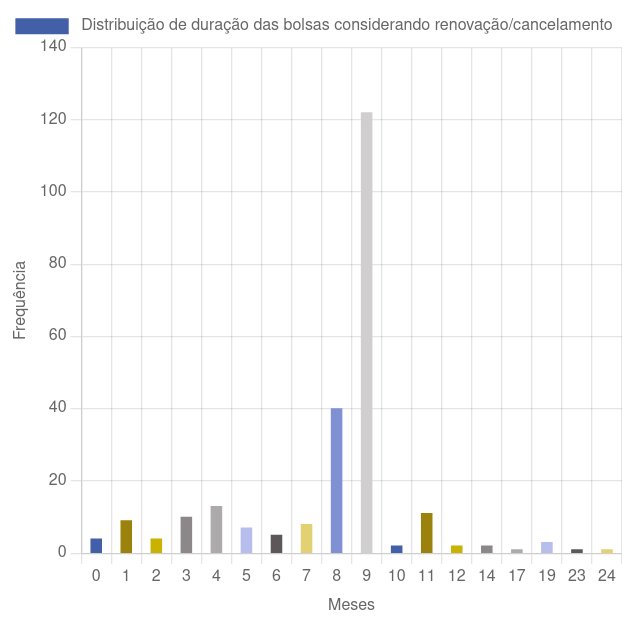
\includegraphics[max size={\textwidth}{\textheight}]{../../../imagens/duracao-bolsas.png}

	\end{center}

	\caption{\label{57dff672d55e14e1a107d4c7f63ccc2759fb6b3a}Histograma de duração das bolsas de iniciação científica (ITI A e ITI B) para o Recorte C, pertinente ao período de 2020 a 2021. (fonte: coordenação do Projeto WASH, com a participação da autora)}

\end{figure}

O histograma da Fig. 44 indica que, para o período de 2020 a 2021, houve uma prevalência de vinculação de bolsistas de iniciação com duração de nove meses, um tempo compatível com o período letivo. O gráfico mostra, também, que muitas bolsas se encerram com poucos meses de concessão, indicando a ocorrência de "turn-over", ou seja, uma relevante rotatividade de bolsistas. Essa situação é normalmente observada no nível de iniciação científica, talvez um resultado das incertezas da adolescência, quando ainda não estão consolidados os interesses profissionais.

Por outro lado, observam-se na Fig. 44 dados que indicam que há estudantes que ficam por mais de um ano como bolsistas do WASH, embora isso ocorra com menor incidência.

A amostra de bolsas de iniciação científica (438), mesmo limitada para o período de 2020 a 2023, coloca o WASH entre os maiores Programas do gênero no Brasil, inclusive quando essa quantidade é comparada com a de grandes universidades públicas brasileiras.

A experiência da autora mostra que essa quantidade de bolsistas requer um grande esforço de gestão, dado que cada bolsista precisa ter associados pelo menos os seguintes elementos: Currículo Lattes, Plano de Trabalho, termo de outorga, coorientador definido, conta no Banco do Brasil, relatório, produção de artigos, participação em oficinas e congressos científicos, produções técnicas, audiovisual e jogos (Scratch).

Além do esforço de gestão dos documentos, há a necessidade de prestação de contas anual, a qual é baseada na avaliação individual de cada bolsista feita pelo orientador em conjunto com o coorientador. Em muitos casos os bolsistas de extensão do Programa (bolsas EXP) colaboram com a avaliação dos resultados. Esta avaliação precisa ser registrada na Plataforma Carlos Chagas do CNPq (CHAGAS, 2022) em cada ciclo de avaliação para cada bolsista.

O registro dos eventos do WASH permite identificar a atuação de uma rede interna, voltada para a organização das atividades. Essa rede é constituída, principalmente pelos  Bolsistas EXP, ADC, ATP e DTI, que são profissionais experientes na prática de extensão. A análise destas atividades mostram que esses profissionais tem o papel de organizar o Programa em suas várias localidades de execução, bem como garantir a multiplicação das oficinas, capacitando novos bolsistas, participando do planejamento com os coordenadores locais, produzindo conteúdos e novas oficinas e trazendo novos parceiros. É também uma atribuição dos bolsistas de extensão, a realização de pesquisa especificada em um plano de trabalho, que visa a produção de conhecimento baseado no método científico.

As atividades descritas acima, que antes eram distribuídas por todos os bolsistas, a partir de 2020, passaram a ser realizadas no âmbito de uma estrutura interna denominada "Frente Multiplicadora", que é um instrumento não formal, heterárquico de mobilização dos trabalhos. A Frente Multiplicadora é coordenada por Ana Carolina de Deus Soares e envolve dezenas de bolsistas de extensão do WASH, em reuniões periódicas.

A descrição acima permite identificar práticas dos bolsistas no WASH que são similares às dos implementadores do GESAC que, também, se organizavam em rede, sem hierarquia, para multiplicar e disseminar o conhecimento em Cultura Digital pelo país. Esse entendimento se sustenta, também, na superposição de bolsistas-chave do WASH que atuaram no GESAC ou em programas associados (Pontos de Cultura), a exemplo desta autora, de Antônio Albuquerque, Rafael Gomes da Cruz (Banto), Michel Alencar Morandi, Vincenzo Tozzi, Andrea Saraiva e Angel Luis.

\subsection[Caracterização dos Planos de Trabalhos e Relatórios]{Caracterização dos Planos de Trabalhos e Relatórios}\label{Caracterização dos Planos de Trabalhos e Relatórios}
Ao receber o termo de outorga, expedido pelo CNPq, o (a) bolsista do WASH, de qualquer modalidade, assume o compromisso de realizar um projeto de pesquisa, além das atividades de extensão. Estas últimas envolvem a participação como multiplicadores das oficinas em escolas de ensino fundamental e demais entidades responsáveis. Em geral, é exigida uma dedicação de 15 horas semanais, das quais 12 horas dedicadas à pesquisa e três horas à multiplicação no ensino fundamental.

As atividades e os "entregáveis" referentes ao projeto de pesquisa são especificadas por meio de um plano de trabalho, apresentado ao CNPq. Dentre os entregáveis definidos nesse Plano de Trabalho, é obrigatório constar o relatório, que é uma forma de documentação científica, que também serve para a prestação de contas.

Assim, um aspecto importante da caracterização do Programa WASH é a contabilização e classificação dos Planos de Trabalho e Relatórios produzidos pelos bolsistas.

Para essa contabilização foram empregados, neste trabalho, os seguintes instrumentos:


\begin{itemize}
\item plataforma Platuóxe, que tem um caráter amostral e não exaustivo em termos de coleta de dados de documentos, particularmente no que diz respeito a números de bolsistas e número de documentos, uma vez que a ferramenta para esse tipo de registro ficou disponível apenas em 2019-2020, como já indicado no capítulo de Materiais e Método;
\item o planejamento financeiro, é um instrumento de compliance, mas que também pode ser utilizado para suprir informações sobre a documentação presente no Programa;
\item o levantamento específico conduzido por esta autora, com base em dados objetivos da Plataforma Carlos Chagas do CNPq, a fonte mais confiável de dados para esse tipo de caracterização; e
\item o levantamento conduzido pela colaboradora do WASH, Giselle Fink, em seu relatório final de pesquisa produzido pela mesma.
\end{itemize}

A Fig. 45 apresenta a distribuição de documentos registrados na Platuóxe referentes ao Recorte B, lembrando que este recorte implica não ter o registro de produção de bolsistas anterior a 2020, quando a respectiva ferramenta ainda não estava disponível. Mesmo como esse caráter amostral, é possível identificar quais são os documentos mais comuns do acervo do WASH. Note-se a existência de uma grande quantidade de documentos com tipos não declarados, uma característica que aponta problemas com a capacitação dos usuários da plataforma Platuóxe. Em muitos casos esses usuários são os próprios bolsistas.



\captionsetup{format=plain}
\begin{figure}[htb]

	\begin{center}

		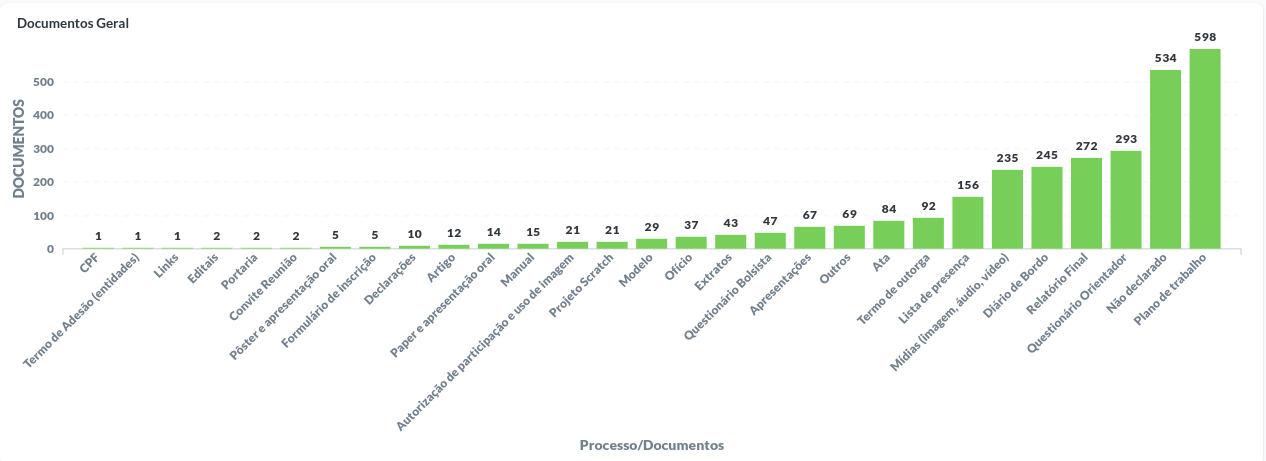
\includegraphics[max size={\textwidth}{\textheight}]{../../../imagens/documentos-gerados.png}

	\end{center}

	\caption{\label{d4bddf3f657cfd53603dfd0dfc92b9c8ba526073}Distribuição de documentos no Programa WASH, segundo o estudo realizado no Recorte B, frisando que este recorte contém registros de bolsistas após 2019-2020, quando o recurso foi integrado à plataforma Platuóxe. (fonte:  [[WASH (2023)]]).}

\end{figure}

Os limites presentes no Recorte B quanto ao registro de documentos e bolsistas indicam que os dados da Fig. 45 são parciais, restringindo-se ao período de 2020 a 2023. Portanto, é razoável considerar que o total de documentos no acervo do WASH é substancialmente maior, uma vez que o Programa se iniciou em 2013.

No que se refere às temáticas dos planos de trabalho, utilizamos os resultados do estudo (FINK, 2022), de caráter amostral, uma vez que é restrito ao período 2020 a 2021 para determinar o perfil de temas do WASH. (FINK, 2022) indica uma prevalência da área "Ciências Exatas e da Terra" (com 46,4\%) em relação a "Ciências Sociais Aplicadas" (com 17,8\%), "Ciências Humanas" (com 17,8\%), "Divulgação Científica" (14,3\%) e "Ciências Biológicas" (com 3,67\%).

Um estudo detalhado das subáreas de conhecimento abordadas pelos planos de trabalho do WASH é apresentado por (FINK, 2022) (ver Fig. 46). Este estudo é restrito ao Processo CNPq 4000172015-6, mas permite avaliar de forma amostral o perfil de temas dos projetos de pesquisa, que mostra uma distribuição com prevalência das temáticas STEAM, ampliada da proposta original do Documento de Referência.



\captionsetup{format=plain}
\begin{figure}[htb]

	\begin{center}

		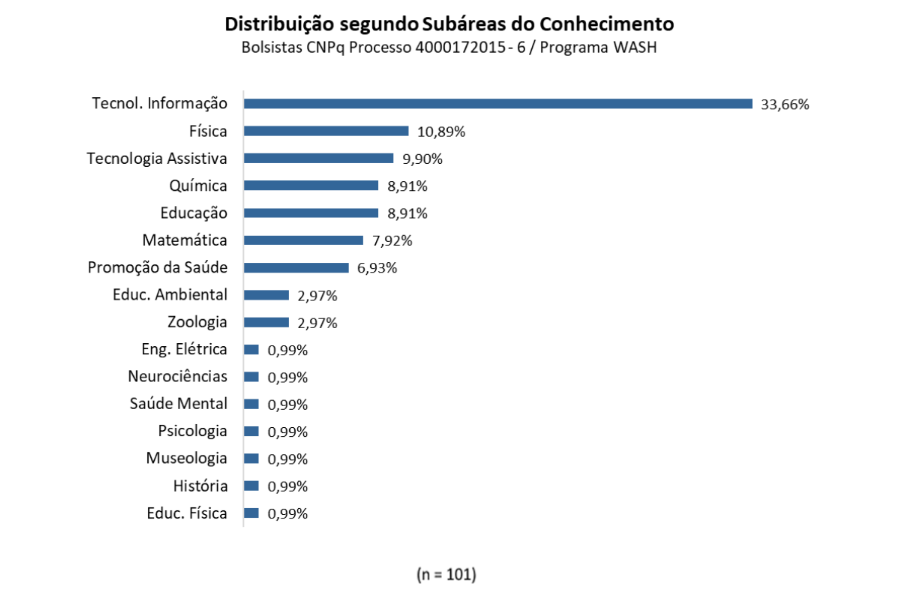
\includegraphics[max size={\textwidth}{\textheight}]{../../../imagens/areas-conhecimento.png}

	\end{center}

	\caption{\label{8700d705d4d270f6322d938a607230e59db00978}Distribuição dos temas de planos de trabalho dos bolsistas de iniciação científica, referentes à emenda parlamentar associada ao Processo CNPq 4000172015-6. (fonte: FINK ,2022)}

\end{figure}

\subsection[Número de eventos realizados]{Número de eventos realizados}\label{Número de eventos realizados}
O número de eventos realizados anualmente é um importante indicador da evolução do Programa WASH, revelando, por exemplo, sua taxa de crescimento ou sua resposta a eventos externos, tais como o isolamento social imposto pela pandemia de COVID19.

Os eventos, como explicitado na seção 2.3 da Fundamentação Teórica, são caracterizados pelo tipo de atividade e o tema trabalhado.

Utilizamos dados obtidos dos Recortes A e B para gerar as Figs. 47 e 48, respectivamente.

A fig. 47, referente ao Recorte A, traz a evolução do número de eventos realizados ao longo dos 10 anos de existência do Programa, ressalvando-se que os dados para o ano de 2022 são parciais, uma vez que esse recorte se encerra em agosto de 2022.



\captionsetup{format=plain}
\begin{figure}[p]

\centering


\begin{minipage}[b]{0.4\linewidth}
        \centering
                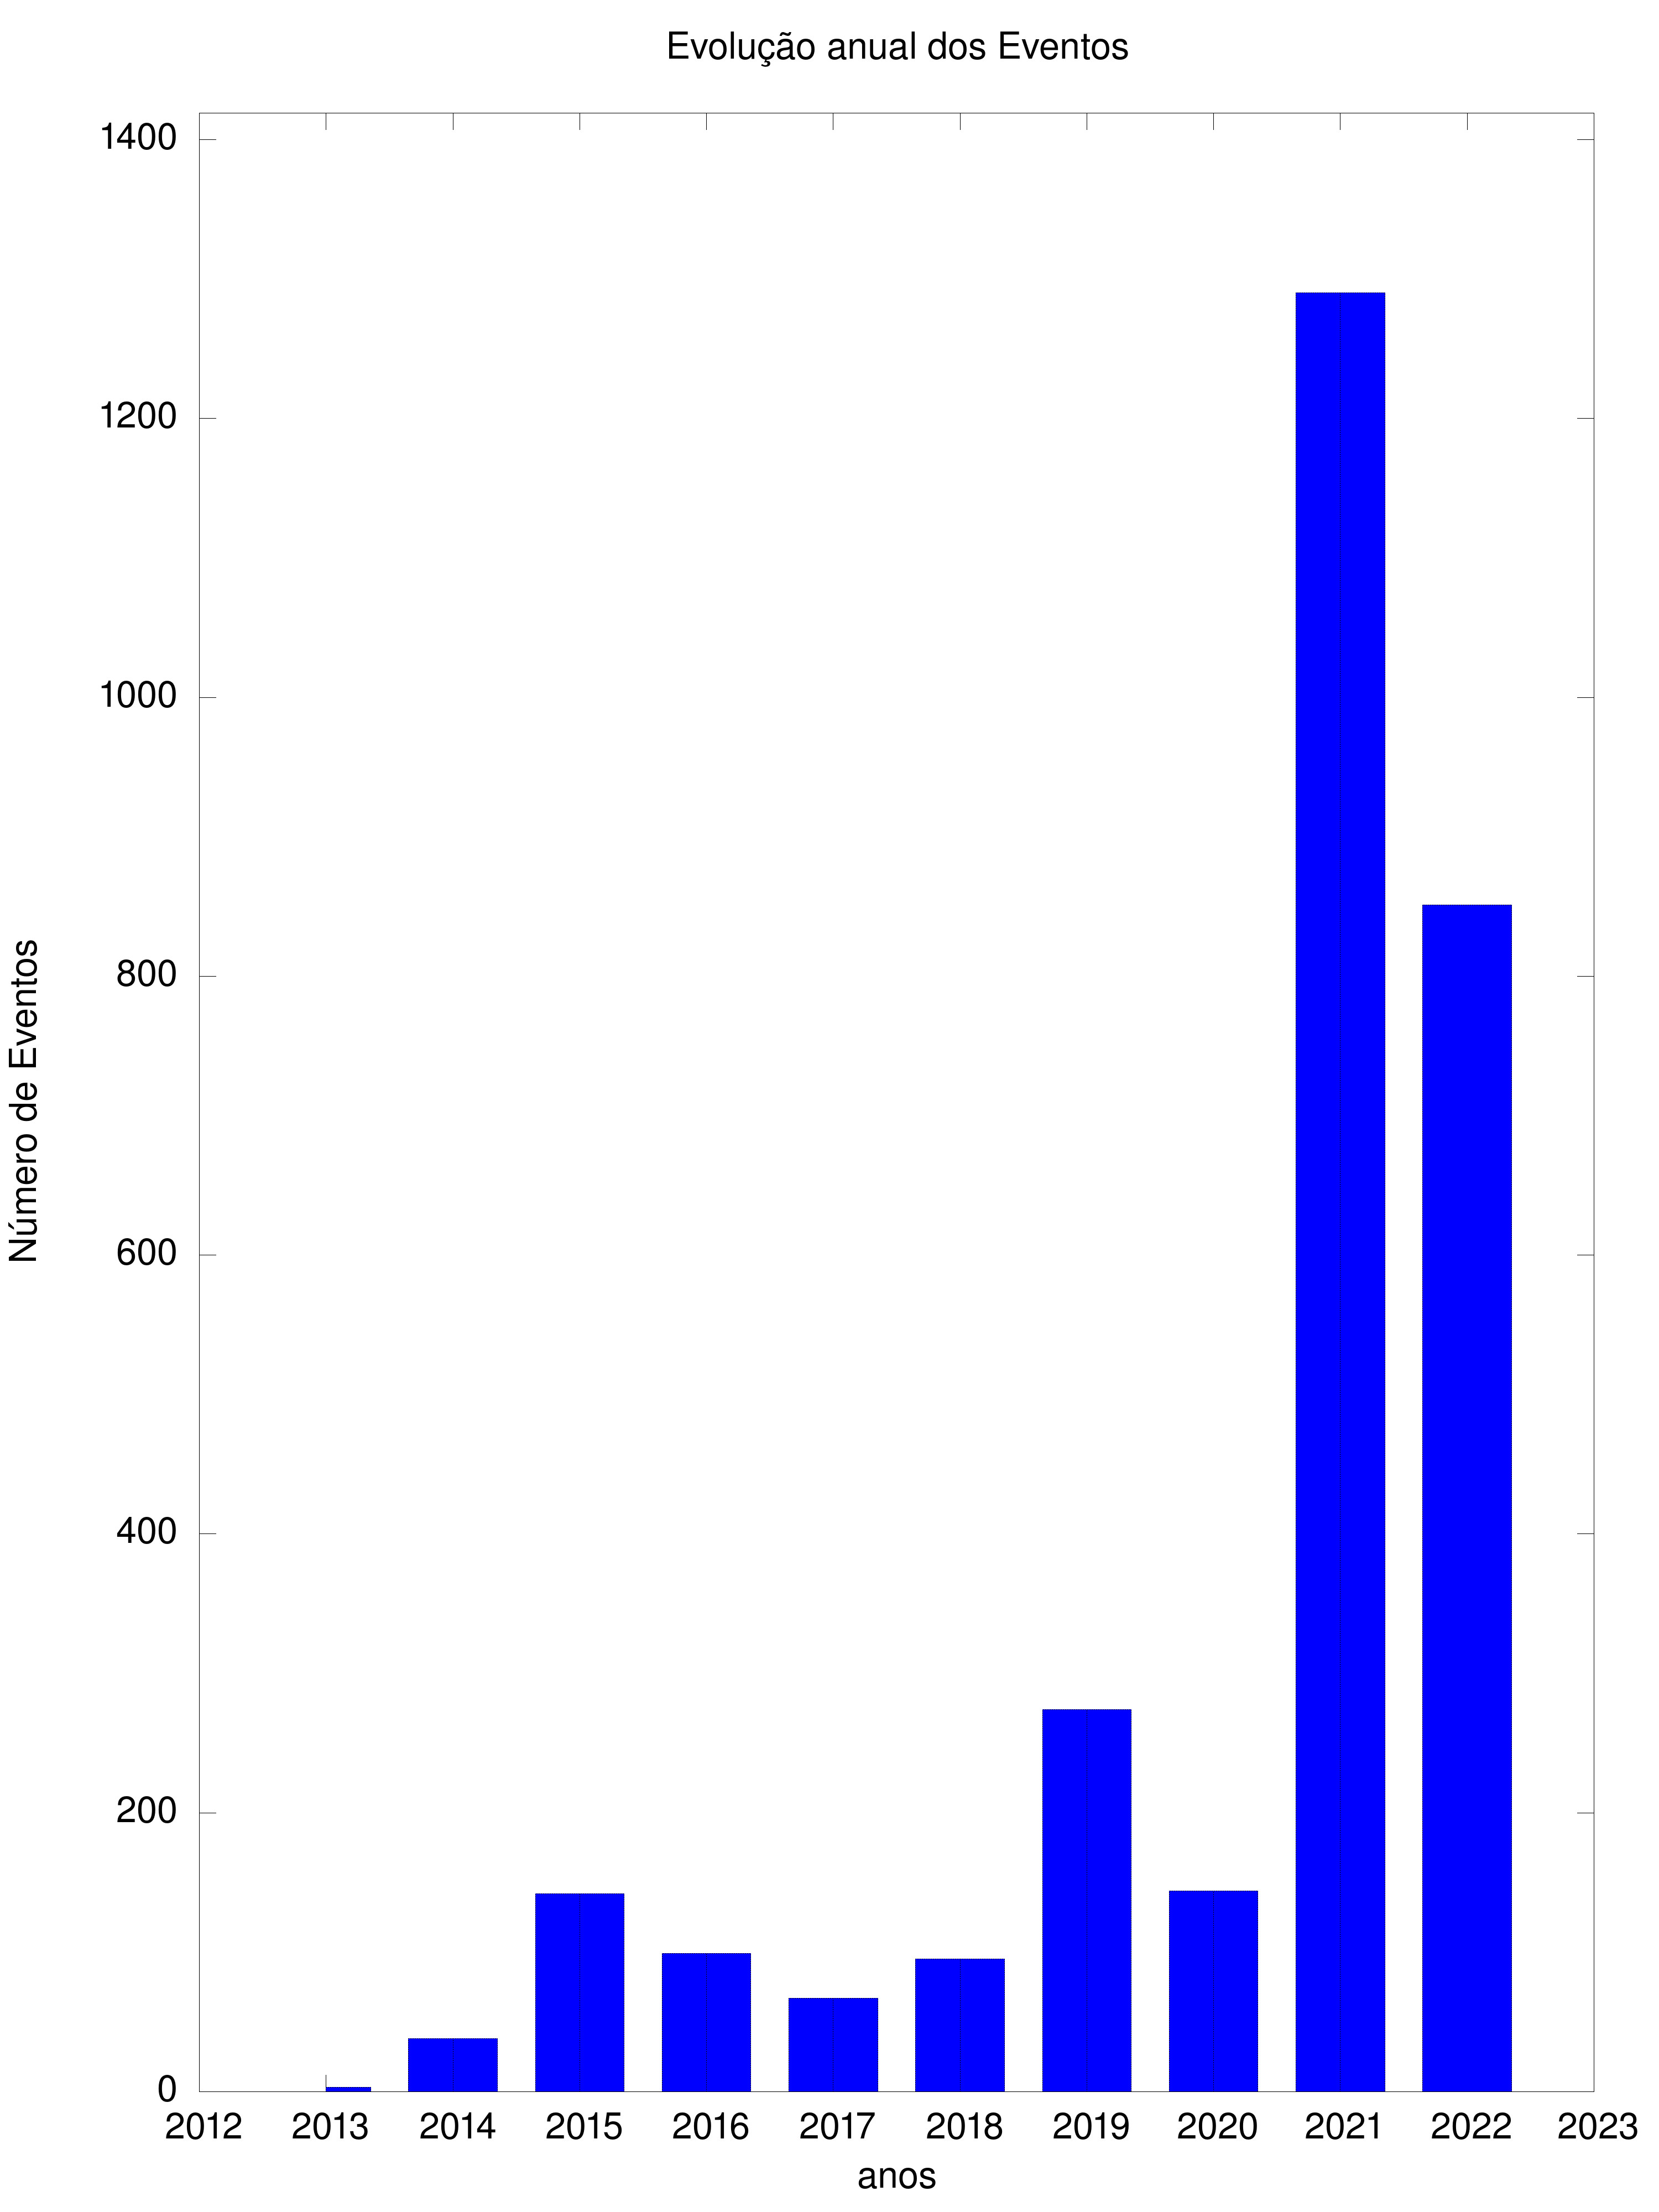
\includegraphics[width=1.0\linewidth]{../../../imagens/output-eventos.jpeg}
                \caption{Evolução anual do número de eventos realizados, obtida a partir do Recorte A. Os dados para 2022 são parciais, uma vez que a atualização foi interrompida em 26 de agosto de 2022.}
                \label{8af5236ba8f91623157f8f95ae10366b416d6049}
\end{minipage}%
\hspace{0.5cm}
\end{figure}



A Fig. 48 é referente ao Recorte B e, portanto, são os dados de janeiro de 2023 que são parciais.



\captionsetup{format=plain}
\begin{figure}[htb]

	\begin{center}

		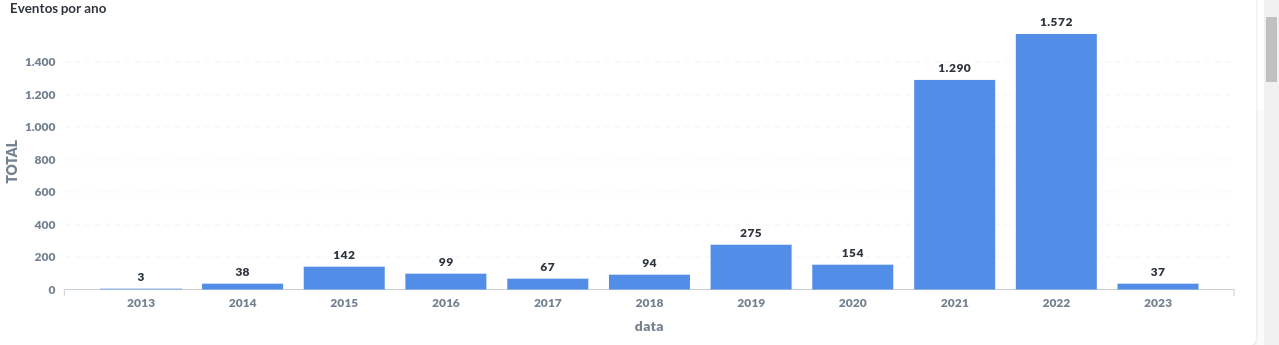
\includegraphics[max size={\textwidth}{\textheight}]{../../../imagens/eventos-ano-recorte-B.png}

	\end{center}

	\caption{\label{06b38fbf8d96a7c692475ebb4c27e84923107c5a}Evolução anual do número de eventos com base no Recorte B. Os dados de janeiro de 2023 são parciais. (fonte:  [[WASH (2023)]])}

\end{figure}

Os gráficos, independentemente do recorte escolhido, indicam um crescimento acentuado do Programa a partir de 2019, com uma interrupção em 2020, decorrente do isolamento social imposto pela pandemia. Decidimos apresentar os dois gráficos para que seja possível avaliar a diferença entre os dados do Recorte A e B. O Recorte B é bem mais completo e indica a realização de 3.771 eventos, ao longo dos 10 anos do WASH.


\noindent\begin{center}\mbox{\centering\fbox{\centering\par\parbox{0.7\linewidth}{\small\textit{O Recorte B indica a realização de 3771 eventos pelo WASH.}\normalsize}}}\end{center}


O comportamento do gráfico de evolução anual dos eventos é semelhante ao comportamento dos gráficos de evolução de participantes e participações, já mostrados na seção 4.2.4. Essa coincidência reforça a interpretação de que o crescimento do Programa foi intensificado pela chegada de novas emendas a partir de 2019, que permitiram a expansão em várias localidades.

Uma análise do Recorte B indicou que cerca de 22,5\% dos eventos referiram-se à programação de jogos com a linguagem Scratch, segundo a declaração dos organizadores de cada evento. Esse número é substancialmente superior ao de qualquer outra temática abordada e pode estar subestimado, dado que depende da declaração dos organizadores.

No que se refere às escolas participantes, ainda dentro do Recorte B, foi possível identificar 50 escolas nominalmente nos registros. A escola E.E. Vitor Meirelles,  localizada em Campinas, se sobressaiu, representando cerca de 11\% dos registros de eventos em escolas.

Dentre as entidades promotoras, se sobressaíram: CTI Renato Archer (16\%), IFSP Jacareí (17\%) e IFSP São José dos Campos (16\%). Esse percentual de participação é em relação aos eventos com registro de entidade promotora.

\subsection[Distribuição etária nos eventos]{Distribuição etária nos eventos}\label{Distribuição etária nos eventos}
Uma das questões fundamentais dessa pesquisa é verificar se o WASH realmente está atingindo o público alvo, declarado em seu documento de referência. Esse público é constituído de crianças e jovens, faixas etárias pertinentes aos ensinos fundamental e médio, respectivamente.

Uma forma de verificar essa eficácia de atendimento é organizar os dados de participação em eventos na forma de um histograma de idades. Essa demanda, especificada pela autora, levou ao desenvolvimento de uma ferramenta de consulta estruturada específica para esse fim, a qual ficou vinculada ao Recorte A.

A Fig. 49 apresenta os histogramas de idade para os anos de 2013 a 2022. Os gráficos estão posicionados lado a lado em uma mesma página, com eixos cujas as escalas são idênticas, para que seja possível acompanhar a evolução da forma de suas distribuições ao longo dos anos do Recorte A.

Antes de analisar a Fig. 49, é preciso enfatizar que os dados que originaram os histogramas são parciais, dado que os cadastros presentes na Platuóxe não estão completos no que se refere ao ano de nascimento dos (as) participantes. Em outras palavras, os dados que geraram os histogramas são um subconjunto da amostra representada pela Platuóxe. A tabela participantes2, onde estão registrados os cadastros, tem apenas uma fração de registros com informação de data de nascimento.

Mesmo com a limitação indicada, as tendências observadas na Fig. 49 permitem compreender melhor a evolução do público alvo do WASH.



\captionsetup{format=plain}
\begin{figure}[htb]

	\begin{center}

		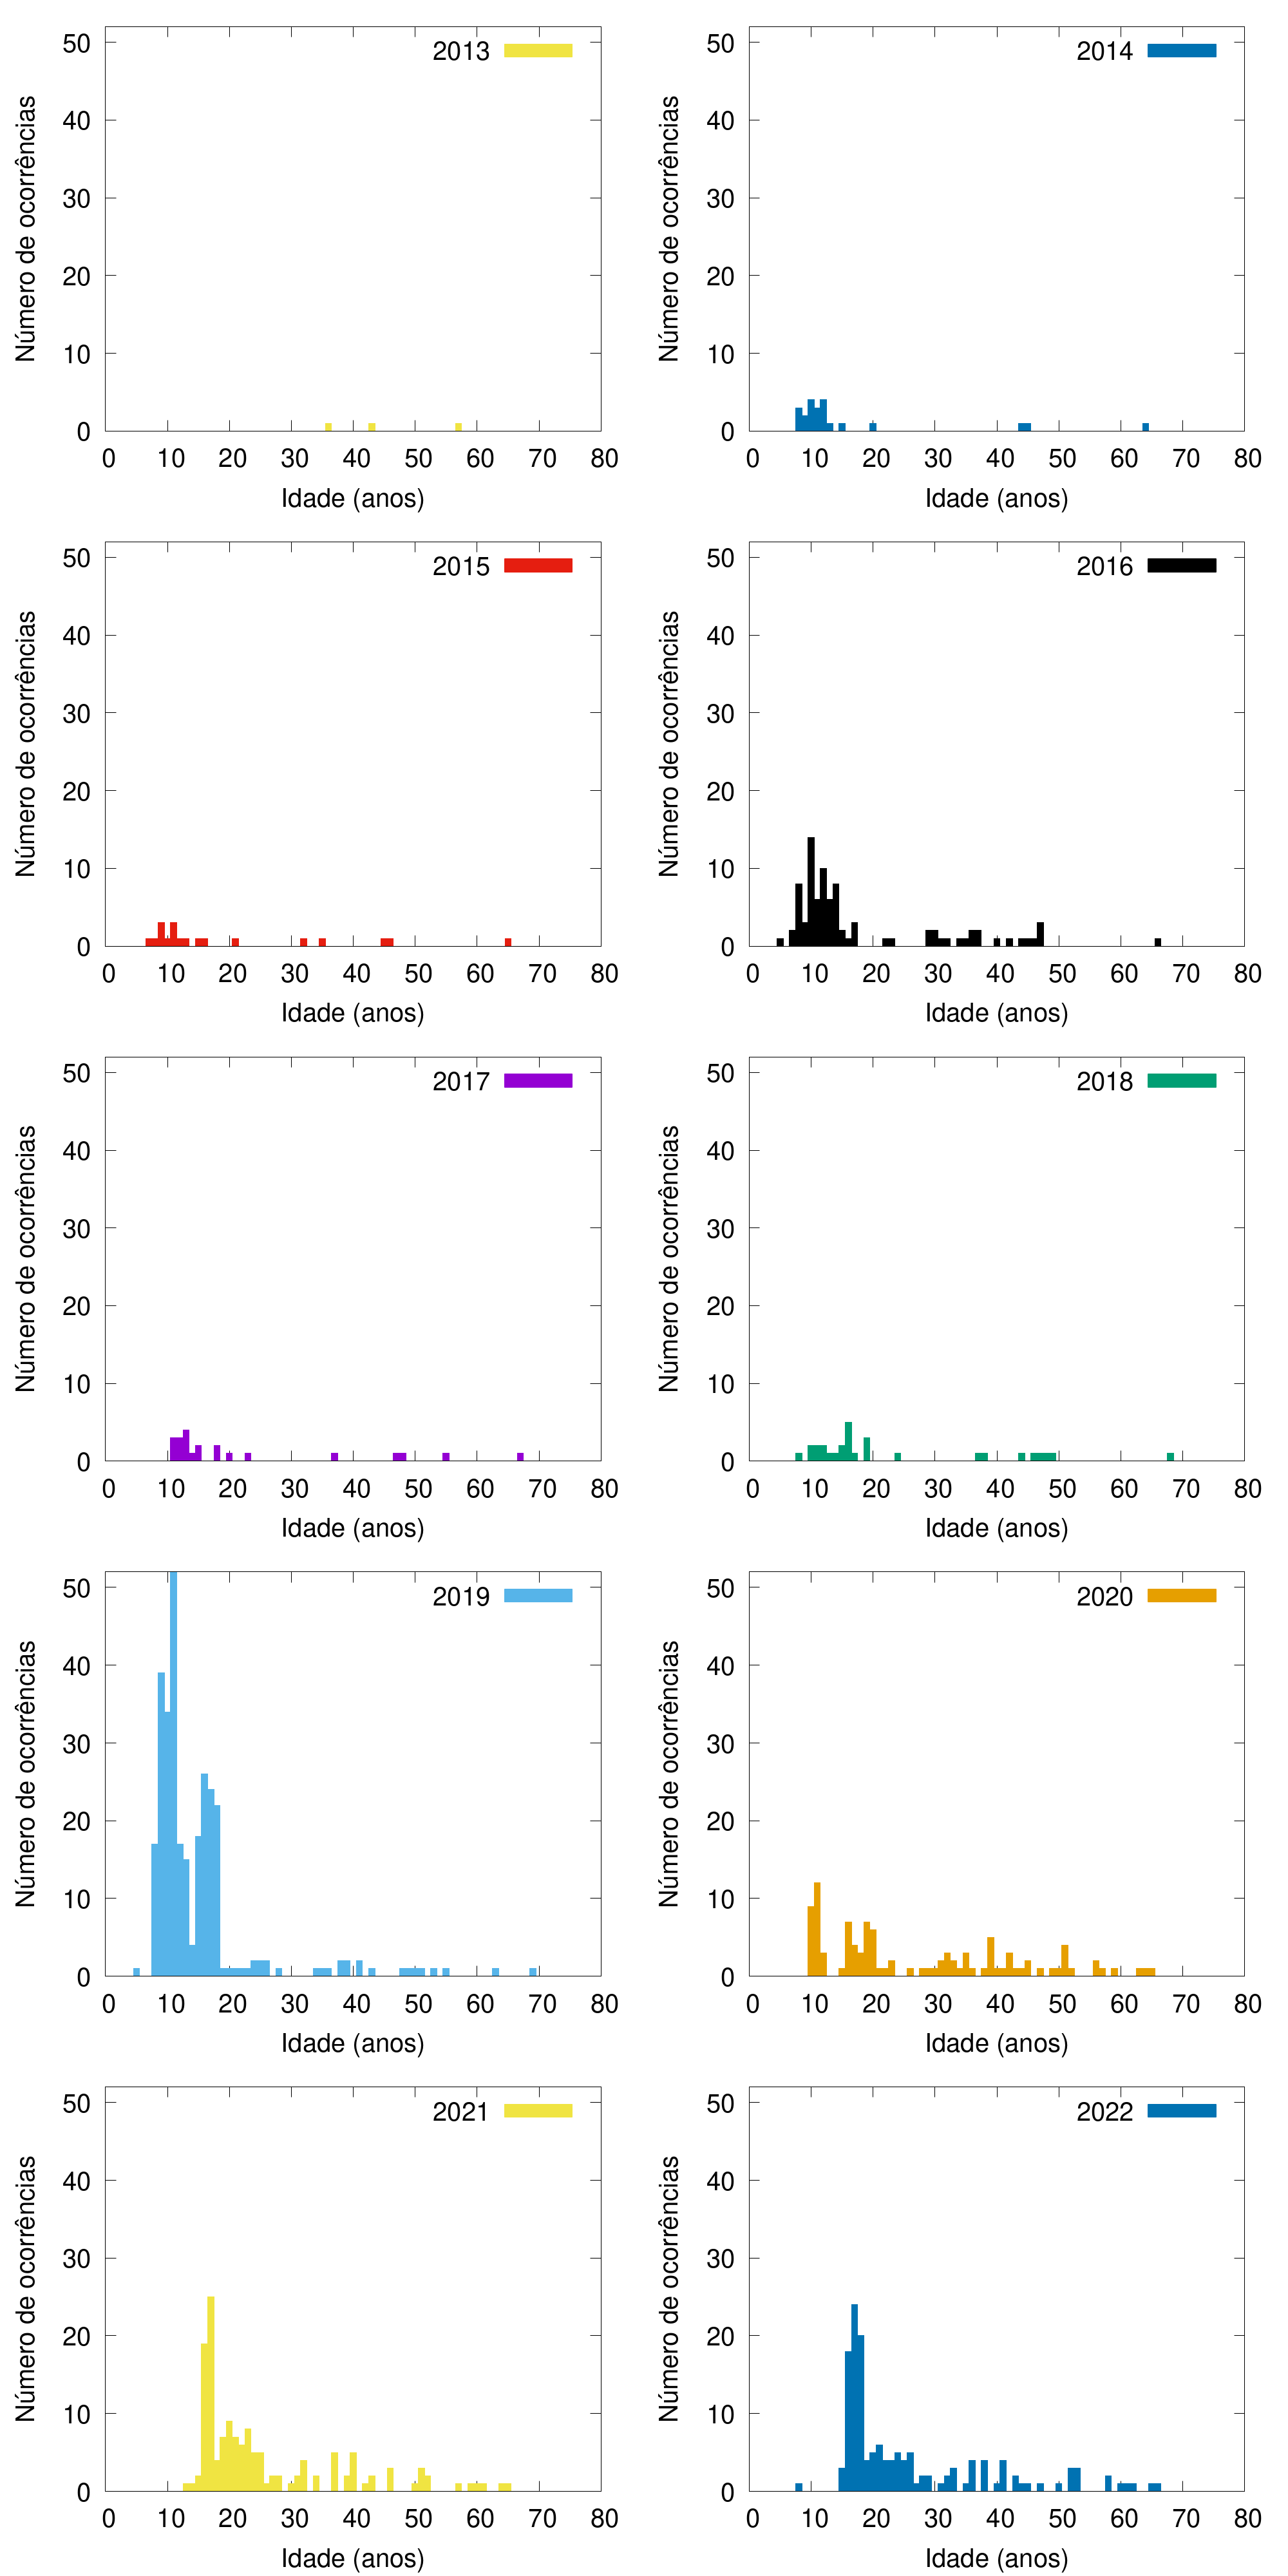
\includegraphics[max size={\textwidth}{\textheight}]{../../../imagens/histograma-de-idades-no-ano-do-evento.png}

	\end{center}

	\caption{\label{978341992d3d49498d48c41acc77f05f08f49ead}Distribuição etária dos participantes, ano a ano.}

\end{figure}

Uma observação cuidadosa dos histogramas da Fig. 49 permitirá concluir que o pico das distribuições etárias está se deslocando para a direita, com a passagem dos anos de execução do WASH.

Esse deslocamento para a direita pode ser interpretado de duas formas:


\begin{itemize}
\item a idade média do público alvo do WASH está aumentando, com o atendimento de cada vez mais educandos jovens; e
\item a coleta de dados do WASH está privilegiando o registro de participantes mais velhos, em detrimento do registro de crianças, mascarando o real perfil etário de atendimento do Programa.
\end{itemize}

\subsection[Distribuição de atividades realizadas nos eventos]{Distribuição de atividades realizadas nos eventos}\label{Distribuição de atividades realizadas nos eventos}
A distribuição de atividades realizadas durante os eventos é apresentada na Tabela 12. Elas podem ser classificadas como "atividade meio", voltadas para garantir o funcionamento do WASH, e "fim", voltadas para o atendimento do público alvo e representam a atividade principal durante o evento, podendo haver outras atividades secundárias, que não estão sendo consideradas.





\begin{table}[htb]
\tiny
\caption{\label{ad56a6a7e392bc429361f174f66a1af09330a2d9}Distribuição dos tipos de atividades realizadas durante eventos do WASH. (fonte: WASH, 2023)}

\centering
\begin{tabular}{|c|c|c|}
\hline
Atividade  &  Tipo  &  \% dos eventos \\
\hline
Apoio a Eventos  &  meio  &  0,13 \\
Apoio a Eventos de CTI  &  meio  &  0,03 \\
Apresentação de Projetos  &  fim  &  0,60 \\
Apresentação sobre o WASH  &  fim  &  3,04 \\
Ativ. Artísticas e Culturais  &  fim  &  0,17 \\
Documentação de desenvolvimento  &  meio  &  0,77 \\
Eventos on-line  &  fim  &  0,30 \\
Oficina  &  fim  &  46,30 \\
Oficina de multiplicação  &  fim  &  1,91 \\
Palestras diversas  &  fim  &  0,17 \\
Participação em Eventos  &  fim  &  0,20 \\
Participacao em Eventos de CTI  &  fim  &  0,37 \\
Realização de Eventos  &  fim  &  0,23 \\
Recepção de Visitas  &  fim  &  0,07 \\
Reunião com a Comunidade Atendida  &  fim  &  0,50 \\
Reunião com Interessados  &  fim  &  7,53 \\
Reunião da Coordenacao Geral  &  meio  &  1,37 \\
Reunião de Equipe  &  meio  &  23,55 \\
Reunião de Orientação aos bolsistas  &  fim  &  8,03 \\
Reunião Frente Multiplicadora  &  meio  &  0,17 \\
Rodas de Conversa  &  meio  &  4,38 \\
Shows Científicos  &  fim  &  0,03 \\
Visita a entidade externa  &  fim  &  0,13 \\
\hline
  &  TOTAL MEIO  &  30,97 \\
  &  TOTAL FIM  &  69,01  \\
  &  TOTAL  &  100,00 \\
\hline
\end{tabular}
\end{table}


A Tabela mostra uma prevalência das atividades fim (69\%) em relação às atividades meio (31\%).

\subsection[Cidades Atendidas]{Cidades Atendidas}\label{Cidades Atendidas}
Com base no Recorte B foi possível levantar a lista de cidades alcançadas pelo WASH, em vários contextos. Este levantamento foi feito por meio de consultas estruturadas, aplicadas à Platuóxe. Cabe relembrar que os dados dessa plataforma são uma amostra do total de atividades efetivamente realizadas pelo WASH.

Na Fig. 50, vemos o gráfico da distribuição dos bolsistas em função das cidades brasileiras onde estão radicados. Por meio de legendas coloridas, o gráfico permite visualizar, simultaneamente, as distribuições de modalidades de bolsas por essas cidades. Note que não se tratam de cidades onde, necessariamente, ocorreram eventos do WASH. As cidades estão ordenadas em ordem alfabética.



\captionsetup{format=plain}
\begin{figure}[htb]

	\begin{center}

		\includegraphics[max size={\textwidth}{\textheight}]{../../../imagens/distribuicao-bolsistas-por-cidades.png}

	\end{center}

	\caption{\label{272b812569e747beabce0484704c884a06f72e19}Distribuição das localidades onde bolsistas do WASH estão radicados. (fonte:  [[WASH (2023)]])}

\end{figure}

A Fig. 51 traz a distribuição de eventos do WASH por cidades brasileiras.



\captionsetup{format=plain}
\begin{figure}[htb]

	\begin{center}

		\includegraphics[max size={\textwidth}{\textheight}]{../../../imagens/eventos-cidades.png}

	\end{center}

	\caption{\label{f08c4c52c76dddcb99c8ad9685858f3c5990432d}Distribuição de eventos do WASH pelas cidades brasileiras. (fonte: WASH ,2023)}

\end{figure}

\subsection[Canal do WASH e a websérie "Ciência e Cultura Vamos Brincar?"]{Canal do WASH e a websérie "Ciência e Cultura Vamos Brincar?"}\label{Canal do WASH e a websérie "Ciência e Cultura Vamos Brincar?"}
O WASH dispõe de um canal na rede social Youtube para a disseminação de sua produção audiovisual, que é uma parte importante do resultado do trabalho dos alunos dos ensinos fundamental e médio. Este canal é designado " Programa WASH " e seu acervo está aberto para acesso ilimitado.

São 427 vídeos carregados no canal desde 14 de dezembro de 2019, quando o canal foi criado. Anteriormente a essa data, os vídeos do WASH eram "carregados" nos canais individuais de membros da equipe.

Segundo o sistema de estatística do próprio Youtube, o canal teve 56.816 visualizações até fevereiro de 2023, divididas entre os 427 vídeos. A produção é muito variada, contendo animações, dicas sobre programação, "stop motion", oficinas, entrevistas, contação de estórias, vídeos tipo "faça você mesmo", músicas, etc.

Consta do acervo do canal "Programa WASH", a edição de nove episódios da websérie "Ciência e Cultura, vamos brincar?" (CCVB). Esse programa, como já explicado na seção 4.1.6, foi criado como forma alternativa de promover a aprendizagem no contexto da pandemia, quando as oficinas presenciais não eram mais possíveis. O CCVB foi concebido por esta autora, que coordenou suas atividades.

A produção do CCVB contou com a participação de dezenas de colaboradores, divididos em três grupos principais (WASHCNPq, 2022):


\begin{itemize}
\item WASH: esforço coordenado pela autora;
\item "Nós somos a Ciência": iniciativa livre, coordenada pelo divulgador científico Will Namen, que posteriormente se integrou à equipe do WASH; e
\item Cia. Bola de Meia: esforço coordenado por Jacqueline Baumgratz e Celso Pan, que posteriormente passaram  a integrar também a equipe do WASH.
\end{itemize}

Foram nove episódios publicados no Youtube, listados a seguir.


\begin{itemize}
\item Episódio 1: Lançamento
\item Episódio 2: Astronomia, ciência e arte
\item Episódio 3: Água, vida, direito, dever e poder
\item Episódio 4: Fauna, flora e fogo
\item Episódio 5: A criança e a ciência
\item Episódio 6: Sistema Solar
\item Episódio 7: Vacina
\item Episódio 8: Mudanças Climáticas
\item Episódio 9: Acessibilidade
\end{itemize}

Posteriormente à estréia no Youtube, mediante solicitação formal, esses episódios foram disponibilizados para TVs Abertas e "a cabo", tendo sido veiculados por VRT, TV Taubaté e TVT.

\section[Linhas de Tempo]{Linhas de Tempo}\label{Linhas de Tempo}
Neste ponto do texto é possível consolidar na forma de "linhas do tempo" os conhecimentos obtidos a partir do emprego dos métodos relacionados aos eixos 1 e 2.

Construímos 3 linhas que são apresentadas nas seções a seguir.

\subsection[Trajetória do Programa WASH]{Trajetória do Programa WASH}\label{Trajetória do Programa WASH}
O mapa da Fig. 52 apresenta, por decênio, os principais fatos que contribuíram para o Programa WASH, com marcos históricos nacionais e internacionais, incluindo o papel desempenhado por pessoas, bem como os contextos que marcaram a trajetória do Programa WASH.



\captionsetup{format=plain}
\begin{figure}[htb]

	\begin{center}

		\includegraphics[max size={\textwidth}{\textheight}]{../../../imagens/Linha-do-Tempo-trajetoria-WASH-1.png}

	\end{center}

	\caption{\label{e12291971a1551c08a11d25104283d4772778aaf}Linha do tempo representando a trajetória do WASH (produção própria)}

\end{figure}

É possível identificar raízes do Programa WASH nas décadas de 60 e 70 do século passado, quando uma comunidade em torno de uma dita "cultura digital" começou a se formar. Nessas décadas é possível encontrar o pioneirismo de José Ellis Ripper Filho, Alfred Volkmer e András G. Vásárhelyl, criadores do primeiro computador digital brasileiro no Instituto Tecnológico da Aeronáutica. Essa iniciativa pioneira em São José dos Campos foi seguida pela criação do "Patinho Feio", marco do desenvolvimento da Computação na Universidade de São Paulo. Foi na década de 60 que a Profa. Dra. Afira Ripper se transferiu para os Estados Unidos, estabelecendo o primeiro contato com a equipe de Papert, no MIT.

A criação dos laboratórios de microeletrônica, tanto na USP como na Unicamp, também são elementos de importância para entender a concepçào do WASH, uma vez que desses laboratórios decorreu a criação do Centro de Tecnologia para a Informática, em 1982, sucedido pelo Centro de Tecnologia da Informação Renato Archer, berço do WASH.

Outro ponto incluído na linha do tempo foi o estudo pioneiro no Brasil, realizado pela Profa. Cecília Baranauskas, em torno da avaliação da aplicação da linguagem LOGO para crianças

No intuito de mostrar as interrelações entre atores envolvidos com a criação dessa "cultura digital", incluímos na linha do tempo a participação do Prof. José Ellis Ripper Filho no conselho do Centre Mondiale, quando esse centro de pesquisa francês era dirigido por Nicholas Negroponte.

Finalmente, incluímos alguns fatos relacionados com a atuação da autora, a exemplo da contribuição para a criação de um sistema pioneiro de gestão para saúde (SOL), ou a participação no Planejamento Estratégico da Casa Civil para adoção do Software Livre pelo Governo Federal, dentre tantos outros.

\subsection[Trajetória de Políticas Públicas]{Trajetória de Políticas Públicas}\label{Trajetória de Políticas Públicas}
Neste ponto apresentamos uma linha do tempo das políticas públicas que, na nossa concepção, são pertinentes ao programa WASH (ver Fig. 53).



\captionsetup{format=plain}
\begin{figure}[htb]

	\begin{center}

		\includegraphics[max size={\textwidth}{\textheight}]{../../../imagens/ Linha-do-Tempo-Politicas-Digitais Publicas-egov-2.png}

	\end{center}

	\caption{\label{435840ce031a949680fc4fef81afb2709efc0253}Linha do tempo representando a evolução das políticas públicas para o setor digital no Brasil (produção própria)}

\end{figure}

A criação do CNPq na década de 50 é o grande marco para toda a área de ciência e tecnologia brasileira. Não poderia ser diferente para o WASH, que depende da estrutura do CNPq para garantir a concessão de suas bolsas e avaliação de seus resultados. Por razões de escala, não foi possível representar na Fig. 53 o momento de criação do CNPq. O primeiro fato registrado na figura é a criação do Ministério da Ciência e Tecnologia, posterior, inclusive, à criação do CTI Renato Archer.

O programa de iniciação científica para o ensino superior do CNPq foi criado em 1988 e posteriormente foi ampliado para o ensino médio. A linha do tempo mostra também o momento em que se iniciaram as discussões sobre governo eletrônico, seguido da criação do GESAC, entre outros programas voltados para o setor digital.

\subsection[Consolidação das linhas de tempo]{Consolidação das linhas de tempo}\label{Consolidação das linhas de tempo}
O mapa da Fig. 54 consolida a história do Programa WASH, através da junção da linha do tempo “Trajetória Programa WASH” com o mapa “Políticas Digitais Públicas”, e integrando dados sobre o desenvolvimento da linguagem SCRATCH.



\captionsetup{format=plain}
\begin{figure}[htb]

	\begin{center}

		\includegraphics[max size={\textwidth}{\textheight}]{../../../imagens/Linha-do-Tempo-WASH-GERAL-4.png}

	\end{center}

	\caption{\label{7f3511906917a26c6f99731c141fb046fe43495d}Consolidação das linhas do tempo do Projeto WASH (produção própria)}

\end{figure}

\section[Validação das hipóteses]{Validação das hipóteses}\label{Validação das hipóteses}
A partir da síntese dos resultados  dos eixos 1 e 2 será realizada  a validação das hipóteses levantadas na introdução.

\subsection[Hipótese 1: Eficiência e Eficácia do WASH]{Hipótese 1: Eficiência e Eficácia do WASH}\label{Hipótese 1: Eficiência e Eficácia do WASH}
Começaremos a validação da Hipótese 1 por meio da abordagem da eficácia, utilizando os resultados do eixo 2, como base para a análise.

Empregaremos como medição de eficácia a capacidade do WASH de atender o público alvo definido em seu Documento de Referência.

O paralelo entre " público alvo " e eficácia busca retirar da análise, neste momento, os indicadores relacionados à eficiência, que serão tratados a seguir (e.g. número de beneficiários do Programa). Nesse raciocínio, consideramos o WASH eficaz caso o público alvo atendido seja aquele especificado no Documento de Referência, comparando a quantidade relativa de crianças (fundamental), jovens (médio e superior) e adultos, independentemente de quantidade absoluta do somatório desses três grupos.

Considerando a linguagem de Peter Drucker (ver Fundamentação Teórica) sobre eficácia, trazida na seção 2.2.1, atingir o público alvo é "fazer a coisa certa", ou seja, cumprir com um objetivo explícito do Programa.

No Documento de Referência (CTI, 2018), que estabelece "o que o WASH gostaria de ter sido", identificamos que deveria haver, no que tange ao público alvo do WASH, uma preponderância dos alunos do ensino fundamental (ver seção 4.2.6) em relação aos alunos do ensino médio e superior.

Pelo lado dos resultados alcançados via eixo 2, que indicam "o que o WASH conseguiu ser", revelamos em que medida o público alvo, explicitado pelo  Documento de Referência foi alcançado. Ou seja, apresentamos indicações da eficácia do WASH. Fazemos isso expondo dois indicadores do Programa com vistas a avaliar sua eficácia, a saber:


\begin{itemize}
\item os histogramas de idades da Fig. 49, oriundos do Recorte A da Platuóxe, indicam picos de participantes na faixa de 10 a 16 anos, entre  2013 e 2019. Não obstante o caráter amostral do Recorte A, porque não traz a totalidade de cadastros, o fato é que tal faixa etária é compatível com um público alvo representativo do ensino fundamental. No entanto, para os anos de 2020 a 2022, identificamos um deslocamento à direita da posição do pico, que chega a 19 anos, em 2022. Essa situação poderia ser um indicativo de perda de eficácia do Programa, dado que seria um sinal de desvio de seu público alvo (i.e. faixa etária acima da almejada). Mas, segundo o que já discutimos na seção 4.2.3, essa tendência de crescimento da idade dos participantes verificada no Recorte A pode estar associada à coleta de dados deficiente, uma vez que a alimentação de dados sobre crianças participantes foi sendo reduzida pelos parceiros. Essa deficiência de coleta de dados foi associada ao advento da LGPD, dentre outros fatores.  Parece-nos que essa situação "distorcida"  da amostra, a partir de 2020, é  mais provável do que um aumento da idade média dos participantes, exceto para o ano de 2020, quando a pandemia pode ter influenciado, também, o perfil do público alvo.
\item a distribuição dos tipos de modalidades de bolsas, mostrada na Fig. 43, obtida do Recorte B da Platuóxe, embora de caráter também amostral, indica uma prevalência de bolsistas de iniciação científica (cerca de 75\%), que têm o papel de ser  multiplicador das oficinas WASH para o ensino fundamental.
\end{itemize}

As duas considerações acima indicam que o WASH tem sido bem-sucedido em focalizar o ensino fundamental como público alvo, o que torna possível validar a primeira parte da Hipótese 1, i.e. eficácia. As evidências de perda de representatividade das amostras, a partir de 2020, sugerem-nos descartar um possível desvio do público alvo do Programa, a menos de um plausível desvio do público alvo restrito a 2020, decorrente da fase inicial do isolamento social da pandemia. Esse comportamento discrepante é compatível com a queda no número de eventos naquele ano, presente tanto na Fig. 47 quanto na Fig. 48.

Na linguagem de Peter Drucker, a eficiência se refere a "fazer do jeito certo", abrindo a porta para traçar um paralelo com a quantidade de eventos realizados, a quantidade de beneficiários e a relação atividade fim/meio. Esse raciocínio reflete a ideia de que se os processos do WASH forem eficientes (i.e. "feitos da forma correta"), mais pessoas serão atendidas com o mesmo recurso financeiro, independentemente dessas pessoas serem parte do público alvo (i.e. ensino fundamental).

O primeiro aspecto para medir a eficiência é considerar o número de cadastros de participantes, oriundo do Recorte A da Platuóxe, que aponta 3.265 pessoas. Mostramos, pela identificação de eventos em que os participantes não foram contabilizados (seção 4.2.3), que este número está subavaliado. O número efetivo de participantes é passível de ser substancialmente maior, não havendo uma forma confiável de apresentar um número consolidado. Por exemplo, o uso das imagens dos eventos para tentar corrigir o número efetivamente registrado na plataforma seria um método muito impreciso, dado que as imagens são parciais.

Seja como for, se considerássemos a quantidade de 3.265 participantes, isoladamente, chegaríamos a uma avaliação de que o WASH é ineficiente no atendimento de pessoas, dado que é um número relativamente pequeno. Por outro lado, essa avaliação não seria justa, dado que sabemos que esse número é subvalorado. O número de visualizações do canal do WASH no Youtube, combinado com o alcance da divulgação do Programa nas TVs abertas e a cabo, tenderia a pender a balança da avaliação para o campo da eficiência, dado que são números bastante expressivos.

Mas, o atendimento preponderante de alunos do fundamental não é o único objetivo expresso no Documento de Referência do WASH. A realização de iniciação científica é um outro aspecto importante. Nesse quesito, o número de bolsistas é outro indicador importante de eficácia, com centenas de participantes, os quais produziram centenas de planos de trabalho, relatórios e audiovisuais, bem como centenas de joguinhos de computador registrados na plataforma do Scratch, do MIT. Entendemos que essa quantidade de produção corrobora com uma avaliação de eficiência do Programa. No campo da eficácia, o perfil de bolsistas, concentrado em torno de alunos do ensino médio (ver seção 4.2.6), indica que o Programa atendeu suas diretrizes originais.

Outro aspecto que pode ser usado para a avaliação da eficiência do Programa é o balanço de atividades, classificadas nos tipos "meio" e "fim". Como vimos na seção 4.2.10, há uma quantidade relativamente grande de atividades fim (cerca de 69\%).

Com tudo isso em consideração, acreditamos ser possível validar a Hipótese 1, tanto no campo da eficácia (público alvo) quanto no campo da eficiência (milhares de beneficiários), com ressalvas para a qualidade da coleta de dados, que ainda não permitiu obter um número consolidado de participantes e participações, dado o caráter amostral dessa coleta. Também o número de visualizações do canal do WASH no ,Youtube, é um tanto questionável, porque os critério de contabilização daquela rede social não é claros. Os dados de espectadores dos canais abertos e de TV a cabo não foram levantados, não havendo uma estimativa validada no momento.

\subsection[Hipótese 2: Orientação a Projetos]{Hipótese 2: Orientação a Projetos}\label{Hipótese 2: Orientação a Projetos}
No que se refere ao emprego de um método de aprendizagem por "orientação a projeto", sentimo-nos confiantes em validar a presente hipótese. Essa validação é possível por conta da expressiva quantidade de bolsas concedidas, resultantes em centenas de relatórios de projeto, publicações científicas, audiovisuais, dentre tantas outras produções ocorridas no contexto dos projetos de cada bolsista. As temáticas de projetos levantadas, em caráter amostral (ver seção 4.2.7), confirmam que os projetos se deram no contexto do STEM, como previsto no Documento de Referência.

\subsection[Hipótese 3: Origem do WASH]{Hipótese 3: Origem do WASH}\label{Hipótese 3: Origem do WASH}
O levantamento historiográfico permite sustentar a validade desta hipótese, porque confirmou a existência de elementos que ligam a origem do WASH a Orogramas pregressos, tais como o GESAC, O OLPC e o PID, inclusive com superposição de atores, métodos de trabalho, objetivos e formas de organização. Também foi possível identificar o trabalho da Profa. Afira Ripper como um dos elementos de inspiração dos métodos do WASH.

\subsection[Hipótese 4: Prática Pedagógica do WASH]{Hipótese 4: Prática Pedagógica do WASH}\label{Hipótese 4: Prática Pedagógica do WASH}
A ênfase em práticas oriundas da pedagogia de Papert está evidente no Programa WASH, principalmente pela prevalência de oficinas voltadas para o uso de programação de computadores (linguagem Scratch).

Muito embora tenha travado contato com o pensamento de Papert, por meio da avaliação do Projeto OLPC (ver seção 4.1.2), um projeto de educação baseado na aquisição de notebooks, o WASH optou por um caminho diferente. Optou por concentrar todo o seu investimento em pessoas, sem propor a compra de equipamentos. Na concepção do WASH, o investimento em pessoas é feito por meio de bolsas do CNPq, aproveitando a infraestrutura e equipamentos já existentes nas escolas e demais entidades responsáveis participantes para otimizar o uso de recursos.  Mesmo com essa diferença em relação ao OLPC, acreditamos que seja possível validar integralmente esta hipótese.

\subsection[Hipótese 5: WASH como proto-política pública]{Hipótese 5: WASH como proto-política pública}\label{Hipótese 5: WASH como proto-política pública}
O WASH se iniciou como uma atividade voluntária de oferta de oficinas de tecnologia para crianças e jovens de baixa renda, aos finais de semana,  sem financiamento. O fato do Programa, mesmo em caráter voluntário, ter sido concebido e executado no seio de uma instituição de pesquisas federal (CTI Renato Archer), abriu uma oportunidade para propor sua evolução para a condição de projeto institucional. O sucesso das atividades foi demandando a repetição dos projetos, ano após ano. A grande quantidade de projetos deu-lhe as características de um programa, embora nunca tenha sido formalizado como tal na esfera federal.  Hoje, pode ser considerado como uma protopolítica pública nacional. Para sustentar essa hipótese, podemos considerar a variedade de documentos formais de adesão ao seu método, emitidos por autoridades públicas, bem como a grande quantidade de emendas parlamentares concedidas. Assim, o WASH não fica restrito ao vínculo com a administração pública federal, estabelecendo pontes com os demais entes federados, com os poderes executivo e legislativo, com as redes de ensino, com os órgãos de fomento científico e com as organizações sociais.

Para que o WASH transite da condição de protopolítica pública, há que se institucionalizá-lo por meio de instrumento jurídico e estruturas  adequados para a criação efetiva de Programas, no âmbito federal.

\subsection[Hipótese 6: WASH como organização heterárquica]{Hipótese 6: WASH como organização heterárquica}\label{Hipótese 6: WASH como organização heterárquica}
Vimos que o WASH não está cristalizado, por meio de instrumento jurídico, no seio de uma instituição federal. A Portaria CTI 178/2018 traz um conjunto de conceitos, uma descrição do método de execução do WASH e da sua organização, sem o poder de vincular qualquer ator da administração pública a esses desígnios.

A adesão ao WASH se dá pela expressão da vontade unilateral de gestores públicos e de parceiros que, ao publicarem termos de adesão ao Documento de Referência, assumem um compromisso com a sociedade de que aqueles desígnios serão seguidos.

Portanto, não existe relação hierárquica entre as entidades aderentes ao "Programa".

Similarmente, o WASH não tem organograma, sendo desenvolvido exclusivamente por bolsistas, cujas obrigações profissionais estão definidas num termo de outorga, expedido pelo CNPq no momento de concessão da bolsa. Portanto, não existe relação hierárquica entre os profissionais, que se organizam para dividir tarefas de forma colegiada, em estruturas que no WASH foram denominadas "frentes", a exemplo da citada "Frente Multiplicadora" (ver seção 4.2.6).

Portanto, à luz do que foi discutido na Fundamentação Teórica sobre as diferenças entre hierarquia e heterarquia, avaliamos que é possível validar a presente hipótese, confirmando que o WASH se organiza na forma de heterarquia.

\chapter[CONCLUSÃO]{CONCLUSÃO}\label{CONCLUSÃO}
O primeiro aspecto que buscamos mostrar nesta dissertação é que o WASH nasceu no bojo de uma tradição particular de programas de educação, alfabetização científica e tecnológica, cultura digital e inclusão social/digital.

Como característica geral, essa tradição tem por pano de fundo a busca pela inserção do indivíduo em sua própria cultura, através da promoção de vivências não padronizadas e não impostas por uma estrutura central.

Em outras palavras, identifica-se nessas tradições a promoção de eventos de interação humana, com ênfase num ideal de justiça social, distribuídos temporalmente e geograficamente, concebidos para garantir que essas interações se deem no contexto da aprendizagem.

Pensando na metáfora do "segundo dilúvio" de Ascott, citado na Introdução, é inevitável traçar um paralelo entre os programas GESAC, PID e OLPC como a "Arca de Noé", que permitiu sobrevivência a esse "dilúvio".

Aliás, na Introdução, antecipáramos uma das conclusões desta dissertação que aqui depois de todo o trabalho,  sentimos-nos mais confiantes em vaticinar:


\noindent\begin{center}\mbox{\centering\fbox{\centering\par\parbox{0.7\linewidth}{\small\textit{A existência do WASH pode  ser compreendida como mais um esforço - mais uma "Arca de Noé" dos novos tempos, que ajuda na sobrevivência e nos prepara para o "dilúvio informacional", identificado por Ascott.}\normalsize}}}\end{center}


Assim,  o WASH compartilha características em comum com os programas GESAC, PID e OLPC, estudados neste trabalho. Dentre estas características podemos enunciar:


\begin{itemize}
\item o foco na aprendizagem e não no ensino;
\item o caráter estritamente público e não vinculado a interesses comerciais;
\item a adoção do lema: "ensinar como pretexto para aprender";
\item o estímulo à produção de conteúdos pelos próprios educandos, respeitando seu protagonismo, em detrimento de um "conteudismo impositivo";
\item o respeito pelas características e realidades locais, sem imposições sobre a forma de atuação;
\item o respeito às lideranças, aos coordenadores que se consolidam na organização e gestão dos trabalhos;
\item a falta de controle centralizado vertical, em que uma ordem consensual impera, estabelecendo-se uma organização heterárquica;
\item a promoção e o uso das tecnologias livres;
\item o método científico como valor fundamental.
\end{itemize}

A noção de que o WASH é um epítome de uma forma de pensar as políticas públicas, se comprova pelo estudo que fizemos de suas origens.

A aplicação do nosso método historiográfico mostrou que o WASH "bebeu na fonte" das iniciativas pregressas citadas, transformando-as para suplantar suas deficiências.  Por exemplo, diferentemente do GESAC, PID e OLPC, o WASH optou por direcionar todos os seus recursos para o investimento em pessoas, por meio de suas atividades, e na forma de bolsas de diferentes modalidades, em detrimento do investimento em equipamentos. Além disso, na busca de mais inclusão, o WASH abdicou integralmente de apostilas, kits educacionais, livros, textos ou outras formas de conteúdo e equipamentos, diferente do GESAC, por exemplo.

Adicionalmente, vimos que a visão sobre ciência do WASH busca ser  simples, acessível, possível: "Ciência é a compreensão que o outro constrói sobre o conhecimento de alguém". No contexto dessa visão, a realização da ciência depende, sobretudo, da capacidade de expressão do indivíduo, que observa o mundo a sua volta, analisa e organiza os conhecimentos existentes, produzindo, em decorrência, a sua própria narrativa sobre o que aprendeu.

Em síntese, pode-se dizer que o WASH iniciou-se como um constructo resultante das impressões que seus criadores tiveram sobre as iniciativas pregressas. O amadurecimento dessas ideias levou a sua concretização, inaugurada por uma primeira oficina,em setembro de 2013, seguida de subsequentes exercícios e  vivências que - oficina a oficina - resultaram num crescente aprendizado sobre o seu método.

Quando seus criadores adquiriram a confiança no que a ideia inicial do WASH foi se transformando decidiram formalizar suas práticas,valores e métodos em conceitos, expressos  no Documento de Referência, cristalizando-o na forma de anexo a uma portaria  ([[CTI, 2018]])  do Centro de Tecnologia da Informação Renato Archer, em 2018.

Não obstante o alcance legal limitado da referida Portaria, a aprovação formal do método pelo CTI Renato Archer, que, na prática, a edição da portaria representava, estimulou outras entidades a adotá-la. Com isso, criou-se, uma protopolítica pública que, como já dito, são "daquelas que são vivenciadas, mas que ainda não estão formalizadas numa lei federal".

Ao longo de todo trabalho, buscamos comparar, com base na Portaria CTI 178/2018, "o que o WASH gostaria de ter sido" com "o que o WASH conseguiu ser", visão obtida da aplicação dos métodos dos eixos História e Indicadores.


\begin{itemize}
\item O WASH conseguiu manter-se fiel ao seu público alvo pelo menos até 2019. Com a chegada da pandemia, em 2020, os indicadores  aduziram um aumento na faixa etária média de seus participantes, possivelmente um resultado da diminuição de oficinas ofertadas em escolas públicas fechadas pelo isolamento social, uma vez que essas instituições ainda não tinham formas contingentes de promover suas atividades.
\item A partir de 2021, os indicadores do Programa revelam um crescimento muito grande no número de atividades ofertadas pelo WASH, mas o deslocamento à direita do pico das faixas etárias permanece, mostrando, em tese, um público com mais idade. A mudança no padrão de coleta de dados do Programa (ver discussão sobre LGPD) indica que esse deslocamento pode estar associado ao desvirtuamento da qualidade da amostra de dados, dificultando a análise apenas com base no cadastro presente na Platuóxe.
\item O WASH conseguiu atender milhares de pessoas no modo presencial. Por outro lado, os dados de participações presenciais,cadastrados na plataforma do WASH Platuóxe - 3.265 pessoas - são amostrais e não refletem a quantidade total de pessoas atendidas. Entretanto, esse número é confiável como valor mínimo absoluto de pessoas atendidas. Certamente, o número de pessoas atendidas é  superior, o que pudemos comprovar identificando eventos para os quais evidências fotográficas comprovaram mais participações do que as efetivamente cadastradas na plataforma.
\item A capacidade de atendimento de pessoas pelo WASH foi substancialmente incrementada com o advento da websérie "Ciência e Cultura, Vamos Brincar?", que além de dinamizar os acessos ao canal "Programa WASH" (que chegou a mais de 56.000 visualizações), permitiu  aumentar o alcance da mensagem do WASH por meio de TV aberta e TV a cabo.
\item O WASH produziu uma profusão de documentos, audiovisuais, artigos científicos e jogos de computador (Scratch), como antecipado pelo Documento de Referência, os quais estão focalizados em temáticas STEAM. Essa produção se deu no âmbito de centenas de iniciações científicas, que permitiram aos beneficiários exercitarem o método científico e a atuação orientada a projetos. Essa constatação indica que houve uma transição da especificação inicial do Documento de Referência, que previa apenas atividades STEM, para a forma STEAM.
\item Os eventos produzidos no WASH apresentam elementos da pedagogia de Papert, complementados por outras ideias. A visão de Papert esteve também presente na própria forma de organização das atividades do WASH, que se deu no formato heterárquico, seguindo ,também, a tradição do GESAC e, em parte, do OLPC.
\item As deficiências das amostras de dados, evidenciadas, no trabalho apontam para a necessidade de rever os processos de coletas de dados do WASH, que devem aprofundar o papel da Plataforma Platuóxe e transferir para os participantes e organizadores locais mais responsabilidade pela entrada de dados. Essa transferência deve introduzir meios de responsabilização automática na eventualidade de não haver compartilhamento de dados pelos participantes, principalmente no que se refere ao registro de presença, temáticas, tipos de atividades, produção e documentos gerados. Para que essa maior plataformização seja aceita pelos partícipes, o WASH deve preparar uma melhor resposta aos desafios da LGPD, aumentando a confiança das entidades responsáveis ao compartilharem suas informações.
\end{itemize}

\chapter[RECOMENDAÇÕES]{RECOMENDAÇÕES}\label{RECOMENDAÇÕES}
O trabalho de historiografia e o levantamento de indicadores, realizados até o momento, permitiram identificar uma série de oportunidades para a melhoria do Programa WASH, as quais elencamos:


\begin{itemize}
\item Melhoria da Plautósh: identificamos que o Banco de Dados da Platuóxe foi realizado sem o prévio estabelecimento de um Modelo Entidade Relacionamento (MER - Modelo Conceitual). Já iniciamos este trabalho de modelagem e, com isso, pudemos identificar aspectos do banco de dados da Platuóxe que estão fora da normatização requerida, a exemplo de tabelas com duplicação de dados (participantes2 e bolsistas). O esforço de modelagem MER deve culminar com a revisão do banco de dados da Platuósh;
\item Com a revisão do modelo de dados do WASH, há que se integrar todos os recortes de dados (A, B, C), bem como dados em planilhas, integrando tudo em um só sistema;
\item Os processos do WASH precisam ser modelados, para promover uma melhoria de qualidade geral no Programa. Recomendamos a utilização do método Business Process Modelling Notation (BPMN), a exemplo do que foi realizado em caráter pioneiro pelo colega Saulo Monteiro, colaborador do WASH (Fig. 55);
\item A modelagem de processos do WASH deve ser integrada ao desenho da Platuóxe, para aumentar a qualidade da coleta de dados, criando mecanismos de responsabilização e premiação para os partícipes, em suas obrigações de entrada de dados;
\item Uma portaria de aprovação do Documento de Referência deve ser publicada por autoridade com competência para tal, após natural revisão colegiada do órgão interessado. A nova portaria, diferentemente da Portaria CTI 178/2018, deve prever delegação para a coleta de dados de cadastro à autoridade que vier a coordenar o WASH, bem como instrumentos para implantação dos mecanismos de segurança previstos na LGPD;
\item Para que se consolide como política pública, o WASH deve procurar um melhor equilíbrio entre hierarquia e heterarquia, uma vez que apenas instrumentos formais da burocracia estatal são capazes de gerar as responsabilizações necessárias para melhorar a coleta e proteção exigidas pela LGPD no contexto federal;
\item No campo da inclusão e da acessibilidade, o WASH precisa atuar para tornar as oficinas mais inclusivas, avaliando em que medida deve permanecer focalizando a linguagem de programa Scratch, que é reconhecidamente inadequada para pessoas com deficiência visual;
\item O WASH deve aumentar sua atenção à questão da equidade de gênero, atuando preventivamente para evitar situações de prevalência de bolsistas do sexo masculino, como a observada na Fig. 41;
\item A recente transferência do coordenador do WASH do CTI para o CEMADEN abriu a oportunidade de integrar as temáticas de desastres naturais, educação ambiental e ciência cidadã ao Programa WASH. Essa integração está sendo estruturada no contexto do ESTEEM, acrônimo que integra seis disciplinas: Environment, Science, Technology, Engineering, Expression. As características do ESTEEM estão descritas em  [[MAMMANA et al. (2022a)]]; e
\item O WASH deve passar a oferecer bolsas de iniciação científica para o ensino fundamental, no contexto de modalidade já existente no CNPq (IC-Júnior).
\end{itemize}



\captionsetup{format=plain}
\begin{figure}[htb]

	\begin{center}

		\includegraphics[max size={\textwidth}{\textheight}]{../../../imagens/bizagi.png}

	\end{center}

	\caption{\label{17b9e2dc78c8926a87c5d8e8c0c9568cb175db59}Modelagem do processo de multiplicação do WASH, realizado por Saulo Monteiro. (fonte: relatório de Saulo Monteiro)}

\end{figure}

\chapter[PRODUTOS EDUCACIONAIS]{PRODUTOS EDUCACIONAIS}\label{PRODUTOS EDUCACIONAIS}
Esta pesquisa gerou vários produtos educacionais que são descritos a seguir:

\section[Vídeo/Entrevista: Papert e Afira Ripper]{Vídeo/Entrevista: Papert e Afira Ripper}\label{Vídeo/Entrevista: Papert e Afira Ripper}
A entrevista com a Profa. Dra Afira Vianna Ripper foi transformada em audiovisual, estando disponível ao público por meio dos links:


\begin{itemize}
\item Parte 1: https://www.youtube.com/watch?v=fMsy7eW8vxU
\item Parte 2: https://www.youtube.com/watch?v=inxixL5iK4I
\end{itemize}

\section[Revisão do Documento de Referência do Programa WASH]{Revisão do Documento de Referência do Programa WASH}\label{Revisão do Documento de Referência do Programa WASH}
Este produto educacional tem por objetivo apresentar, após anos de prática e de validação do método WASH, uma versão atualizada do Documento de Referência constante na Portaria nº 178/2018/SEI-CTI, de 12 de novembro de 2018.

A revisão teve, como finalidade:


\begin{itemize}
\item melhorar as condições de disseminação da prática do WASH, ampliando sua adoção por escolas públicas;
\item contribuir com a disseminação do método científico, facilitando o acesso a atividades de turno e contraturno voltadas para STEAM;
\item adaptar o Programa WASH a situações de isolamento social, prevendo atividades remotas;
\item promover uma melhor equidade na seleção de bolsistas, evitando situações de prevalência masculina, como a observada no Processo 40001720150-6 (ver Fig. 41).
\item melhorar o processo de coleta de dados do WASH, para garantir indicadores com maior qualidade;e
\item incluir as temáticas de prevenção de desastres naturais, educação ambiental e ciência cidadã, por meio da adoção das práticas ESTEEM, definas em  [[MAMMANA et al. (2022a)]].
\end{itemize}

Identificamos esta necessidade de revisão porque, ao longo de uma década de execução do Programa, observamos um crescente interesse, por parte de outras instituições, pela reprodução do WASH.

\chapter[REFERÊNCIAS]{REFERÊNCIAS}\label{REFERÊNCIAS}
\begin{flushleft}
[AFIRA, 2013] Afira, V.R.; Damin, M.A. da S. A Pesquisa e a Tecnologia na Formação Docente, Prefeitura Municipal de Campinas, 2013
\end{flushleft}


\begin{flushleft}
[ALVAREZ, 2015] Alvarez, C.S. O projeto "Um computador por Aluno" no Brasil: uma história e experiência por concluir, Tese de Doutorado, Universidade Federal do Rio Grande do Sul, 2015
\end{flushleft}


\begin{flushleft}
[ANDRADE, 2022] Andrade, F.S. Tudo que você sempre quis saber sobre a urna eletrônica Brasileira, 1a. Edição, São José dos Campos, SindCT, 2022
\end{flushleft}


\begin{flushleft}
[ARPANET, 2022] Verbete Arpanet na wikipedia
\end{flushleft}


\begin{flushleft}
[BAOBAXIA, 2003] https://baobaxia.mocambos.net/
\end{flushleft}


\begin{flushleft}
[BARRIOS, 2015] Barrios, J.E.R. Information, Genetics and Entropy, Principia 19(1): 121–146 (2015)
\end{flushleft}


\begin{flushleft}
[BATES, 2014] BATES COLLEGE, How to Write a Paper in Scientific Journal Style and Format, v.10-2014, acessado em: https://www.bates.edu/biology/files/2010/06/How-to-Write-Guide-v10-2014.pdf, 2022
\end{flushleft}


\begin{flushleft}
[BBC, 2012] Minitel: The rise and fall of the France-wide web, acessado em 17/11/2022, https://www.bbc.com/news/magazine-18610692, BBC, 2012
\end{flushleft}


\begin{flushleft}
[BELL, 1973]  BELL, 1973, professor de Harvard, que a partir do texto The Coming of Post Industrial Society, Nova York: Basic Books, 1973
\end{flushleft}


\begin{flushleft}
[BENTIVOGLIO, 2010] BENTIVOGLIO, J. História e narrativa na Historiografia alemã do século XIX Anos 90, Porto Alegre, v. 17, n. 32, p.185-218, dez. 2010
\end{flushleft}


\begin{flushleft}
[BERTALANFFY, 1968] Bertalanffy, L. von Teoria Geral de Sistemas, Tradução de Francisco M. Guimarães, 2a. edição, Editora Vozes, 2006
\end{flushleft}


\begin{flushleft}
[BLACK, 2001] Black, E. IBM and the Holocaust: The Strategic Alliance between Nazi Germany and America's Most Powerful Corporation, Dialog Press, 2001
\end{flushleft}


\begin{flushleft}
[BRASIL, 2002] https://antigo.mctic.gov.br/mctic/opencms/legislacao/portarias/Portaria\_MC\_n\_256\_de\_13032002.html?searchRef=gesac
\end{flushleft}


\begin{flushleft}
[BRITANNICA, 2022] Verbee Differential Analyser
\end{flushleft}


\begin{flushleft}
[BRITANNICA, 2022a] Verbete STEM education
\end{flushleft}


\begin{flushleft}
[BRUDNER, 2022] Brudner, E. Twenty Two Advantages and Disadvantages of Using Spreadsheets for Business, acessado via https://blog.hubspot.com/sales/dangers-of-using-spreadsheets-for-sales em 20 de setembro de 2022.
\end{flushleft}


\begin{flushleft}
[BURKE, 1991] Burke, P. A Revolução Francesa da historiografia: a Escola dos Annales 1929-1989 / Peter Burke; tradução Nilo Odália. – São Paulo: Editora Universidade Estadual Paulista, 1991
\end{flushleft}


\begin{flushleft}
[BYBEE, 2010] Bybee, R. W. Advancing STEM Education: A 2020 Vision, Technology and Engineering Teacher, v70 n1 p30-35 Sep 2010
\end{flushleft}


\begin{flushleft}
[BYBEE, 2013] Bybee, R.W. STEM education, challenges and Opportunities, publicado pela National Science Teachers Association, 2013
\end{flushleft}


\begin{flushleft}
[CANALTECH, 2022] SITE https://canaltech.com.br/empresa/ifood/ acessado em 6 de janeiro de 2023
\end{flushleft}


\begin{flushleft}
[CARDOSO, 2014] Cardoso, C.P. Organizações, Sistemas e Métodos (OSM), Univerisdade Federal de Juiz de Fora
\end{flushleft}


\begin{flushleft}
[CASTILHO, 2008] Castilho, C. A ‘heterarquia” , a nova palavra da moda na transição da imprensa para a era digital, Monitor da Imprensa em Observatório da Imprensa, acessado em 28 de novembro de 2022, https://www.observatoriodaimprensa.com.br/codigo-aberto/a-heterarquia-a-nova-palavra-da-moda-na-transicao-da-imprensa-para-a-era-digital/
\end{flushleft}


\begin{flushleft}
[CATTERALL, 2017] CATTERALL, L.G. A brief history of STEM and STEAM from an Inadvertent Insider, The STEAM Journal, V 3(1) 2017
\end{flushleft}


\begin{flushleft}
[CGEE, 2010] Avaliação do PIDs
\end{flushleft}


\begin{flushleft}
[CGEE, 2010a] Mammana, V.P. et al. Produto No. 4 do Contrato CGEE no. 224/2009 - Projeto de Avaliação do Programa de Inclusão Digital, 2009.
\end{flushleft}


\begin{flushleft}
[CHAGAS, 2022] Plataforma Carlos Chagas, 2022
\end{flushleft}


\begin{flushleft}
[CHIBENI, 2006] Chibeni, S.S. Algumas observações sobre o Método Científico, Notas de aula 12/2006
\end{flushleft}


\begin{flushleft}
[CIBERNECTZOO, 2010] The logo turtle - Seymour Papert et al., postado em 10/01/2010, acessado em http://cyberneticzoo.com/cyberneticanimals/1969-the-logo-turtle-seymour-papert-marvin-minsky-et-al-american/ em 23/11/2022
\end{flushleft}


\begin{flushleft}
[CIPOLI, 2012] Cipoli, P. O que é a Lei de Moore, 2012, acessado em 17/11/2022 https://canaltech.com.br/mercado/O-que-e-a-Lei-de-Moore/
\end{flushleft}


\begin{flushleft}
[CNPq, 2020] Mammana, V.P. et al. Relatório CNPq Processo 405240/2017-1, 2020
\end{flushleft}


\begin{flushleft}
[CNPq, 2020a] Mammana, V.P. et al. Relatório CNPq Processo 44412120188, Coordenador Victor Pellegrini Mammana, 2020
\end{flushleft}


\begin{flushleft}
[CNPq, 2020b] Mammana, V.P. Relatório de Prestação de Contas para o CNPq da emenda Parlamentar do Deputado Ivan Valente, Processo 401040/2020-8, 2020
\end{flushleft}


\begin{flushleft}
[CODD, 1970] Codd, E.F. A Relational Model of Data for Large Shared Data Banks, Communications of the ACM, V13, N6, 1970
\end{flushleft}


\begin{flushleft}
[CONGRESS, 1998] 1998 Biennial Report to The United States Congress, Committee on Equal Opportunities in Science and Engineering, 1998
\end{flushleft}


\begin{flushleft}
[COSTA e SILVA, 2019] Costa, A.S.M.; Silva, M.A.C. A pesquisa História em Administração: uma proposta para Práticas de Pesquisa, DOI 10.13058/raep.2019.v20n1.1104, Administração: Ensino e Pesquisa (RAEP) – v. 20, n. 1, 2019
\end{flushleft}


\begin{flushleft}
[CRISTINA, 2005] Cristina, L. Brasil vai avaliar projeto norte-americano de distribuição de computadores baratos, EBC, acessado em http://memoria.ebc.com.br/agenciabrasil/noticia/2005-06-28/brasil-vai-avaliar-projeto-norte-americano-de-distribuicao-de-computadores-baratos, 2005
\end{flushleft}


\begin{flushleft}
[CRUMLEY, 1995] Crumley, C.L. Heterarchy and the Analysis of Complex Societies, Archeological Papers of the American Anthropological Association, Number 6, 1995
\end{flushleft}


\begin{flushleft}
[CTI, 2018] Portaria CTI 178/2018.
\end{flushleft}


\begin{flushleft}
[DANTAS, 1988] DANTAS, V. Guerrilha Tecnológica, Livros Técnicos e Científicos, janeiro de 1988
\end{flushleft}


\begin{flushleft}
[DA SILVA, 2017] DA SILVA, A. S. Heterarquia na Aprendizagem Coletiva e Desenvolvimento de Competência Profissional Pericial num Centro de Criminalística: O Caso da Polícia Militar do Rio de Janeiro, Dissertação de Mestrado, Universidade Federal Rural do Rio de Janeiro, Orientador: Beatriz Quiroz Villardi, 2017
\end{flushleft}


\begin{flushleft}
[DINIZ, 2009] Diniz, E.H. O governo eletrônico no Brasil: perspectiva histórica a partir de um modelo estruturado de análise, RAP — RIO DE JANEIRO 43(1):23-48, JAN./FEV. 2009
\end{flushleft}


\begin{flushleft}
[DOSSE, 2012] Dosse, F. História do tempo presente e historiografia, Tempo e Argumento, Revista do Programa de Pós-Graduação em História, Florionópolis, v. 4, n. 1, p. 5-22, jan/jun 2022
\end{flushleft}


\begin{flushleft}
[DUTTON, 2004] DUTTON, W. Social Transformation in an Information Society: Rethinking Access to You and the World, UNESCO 2004, Society: Rethinking Access to You and the World, 
\end{flushleft}


\begin{flushleft}
[ENCTI, 2016] Estratégia Nacional de Ciência, Tecnologia e Inovação 2016/2022, Ciência, Tecnologia e Inovação para o Desenvolvimento Econômico e Social, Ministério da Ciência, Tecnologia, Inovações e Comunicações
\end{flushleft}


\begin{flushleft}
[ENGLEBART, 2017] ENGLEBART, D. Microeletronics and the art of similitude, 1960 IEEE International Solid-State Circuits Conference. Digest of Technical Papers, 10-12 de fevereiro de 1960
\end{flushleft}


\begin{flushleft}
[FAVERSANI, 1998] Faversani, F. Popper, ciência e história antiga, SÍNTESE NOVA FASE V . 25 N . 83 (1998): 527-550
\end{flushleft}


\begin{flushleft}
[FINK, 2022] Fink, G. Relatório Técnico: Estudo Qualitativo e Quantitativo dos projetos desenvolvidos por bolsistas do Programa WASH - 2019/2020, apresentado ao CNPq em 2022.
\end{flushleft}


\begin{flushleft}
[FIRAT, 1987] Firat, A.F. Historiografia, Método Científico e Eventos Históricos Excepcionais, NA Advances in Consumer Research Volume 14, 1987, Pág. 453-438
\end{flushleft}


\begin{flushleft}
[FREITAS, 2019] FREITAS, I. TEORIAS DA HISTÓRIA NA HISTORIOGRAFIA DE RANKE, Ponta de Lança, São Cristóvão, v. 13, n. 25, jul. - dez. 2019.
\end{flushleft}


\begin{flushleft}
[FULLER, 2011] Fuller, R. Advantages and hazards of using Microsoft Excel to Organize and display water quality data, Proceeedings of the 2011 Georgia Water Resources, held April 11-13, 2011 at the University of Georgia.
\end{flushleft}


\begin{flushleft}
[GODOI et al., 2006] Godoi, C. K.; Bandeira-de-Mello, R.; Silva, A.B. Introdução Pesquisa qualitativa e o debate sobre a propriedade de pesquisar in Pesquisa Qualitativa em estudos Organizacionais - Paradigmas, Estratégias e Métodos, 2a. Edição, Editora Saraiva, 2006
\end{flushleft}


\begin{flushleft}
[GONZALES e KUENZI, 2012] Gonzalez, H.; Kuenzi K. J. Science, Technology, Engineering, and Mathmatics (STEM) Education: A Primer, Paperback, Kindle - August 10, 2012
\end{flushleft}


\begin{flushleft}
[HARARI, 2018]  HARARI, Y. 21 Lições para o século 21, Companhia das Letras, 2018
\end{flushleft}


\begin{flushleft}
[HIRAGA et al., 2006] Hiraga, C.Y.; Andrade, E.C.; Diz, M.A.R.; Tinos, S.H. Um computador por criança - Ergonomia no uso de computadores (1B), 11 de outubro de 2006
\end{flushleft}


\begin{flushleft}
[JANKOSKI, 2017] Jankoski, T. STEM— A Rebranded Idea of the Past, acessado em 10/02/2023 em https://blog.stemscopes.com/stem-a-rebranded-idea-of-the-past, 2017
\end{flushleft}


\begin{flushleft}
[KARA-JUNIOR, 2014] KARA-JUNIOR, N. Estrutura, estilo e escrita de artigo científico: a maneira com que pesquisadores reconhecem seus pares, Revista Brasileira de Oftalmologia 73(5), Set-Out 2014.
\end{flushleft}


\begin{flushleft}
[KIESER, 1994] Kieser, A. Why Organization Theory Needs Historical Analyses - And How This Should be Performed, Organization Science, V. 5, N. 4, November 1994
\end{flushleft}


\begin{flushleft}
[KIJIMA et al., 2021] Kijima R., Yang-Yoshihara M., Maekawa M. Using design thinking to cultivate the next generation of female STEAM thinkers, International Journal of STEM Education (2021) 8:14 https://doi.org/10.1186/s40594-021-00271-6
\end{flushleft}


\begin{flushleft}
[KIMPARA et al., 2023] Kimpara, E.T. et al., Guia Prático: Emendas Parlamentares, UNESP acessado em 3 de fevereiro de 2023 em www2.unesp.br/Home/propeg/emendas.pdf
\end{flushleft}


\begin{flushleft}
[LEVY, 2000] LEVY, P. Cibercultura. 2 ed. Editora 34,  Rio de Janeiro:, 2000.p. 14 e 15.
\end{flushleft}


\begin{flushleft}
[LONGHI, 2009] Longhi, R.R. Videotexto como precursor do jornalismo nos novos meios, Vol.3, no. 2, Dezembro, 2009, www.ppgcomufjf.bem-vindo.net/lumina
\end{flushleft}


\begin{flushleft}
[MAMMANA et al., 2022] Mammana V.P., Tozzi E.S., Cruz R.G. da, Soares A.C. de D., Diogo C.P.M. e Morandi M.A. Memorando no. 70/2021/CEMADEN solicitando Registro de Software Desenvolvido em 2020, 25 de fevereiro de 2022.
\end{flushleft}


\begin{flushleft}
[MAMMANA et al., 1990] Mammana, V.P.; Pereira, R.R.; Mammana G.P. Patente: Modelo de Utilidade. Número do registro: PI9006074, título: "Sistema Eletrônico de Pesquisa de Opinião Pública e Escrutínio" , Instituição de registro: INPI - Instituto Nacional da Propriedade Industrial. Depósito: 23/11/1990
\end{flushleft}


\begin{flushleft}
[MAMMANA et al., 2022a] Mammana, V.P. Disaster risk awareness through ESTEEM education in Ciências Ambientais - estudos e inspirações em Educação Ambiental e Sustentabilidade, organizado por Giovano Candiani e Letícia Viesba, V e V Editora, 2022
\end{flushleft}


\begin{flushleft}
[MAMMANA e TOZZI, 2018] Avaliação do Programa OLPC, Cubatão 2018
\end{flushleft}


\begin{flushleft}
[MAMMANA, 2020] MAMMANA, A. Seminário - Documentação em Ciência e Tecnologia, vídeo do Youtube, https://www.youtube.com/watch?v=-ek\_EjIDWnE acessado em 12/08/2022
\end{flushleft}


\begin{flushleft}
[MAMMANA, 1999] Mammana, C.Z. The Natual History of Information Processors in: The Quest for a Unified Theory of Information, Edited by Wolfgang Hofkirchner, Viena University, Austria, Gordon and Breach Publishers, 1999
\end{flushleft}


\begin{flushleft}
[MAMMANA, 2005] Mammana, V.P. Apresentação do Laptop de U$100 em Túnis, Relatório G apresentado à força tarefa da Presidência da República, 2005
\end{flushleft}


\begin{flushleft}
[MAMMANA, 2006] Mammana, V.P. Relatório A: Educação, Mídia e Displays - Um computador por Aluno, relatório apresentado à Presidência da República, acervo de Victor Mammana, 2006
\end{flushleft}


\begin{flushleft}
[MAMMANA, 2005a] Mammana, V.P. Um computador por criança - Escopo de atuação e revisão da proposta OLPC, 2005
\end{flushleft}


\begin{flushleft}
[MAMMANA, 2018] Mammana, V.P. As origens da vocação de Campinas em Tecnologia da Informação, Correio Popular de Campinas, 04/07/2018, acessado em 20222 através de https://correio.rac.com.br/as-origens-da-vocac-o-de-campinas-em-tecnologia-da-informac-o-1.707672
\end{flushleft}


\begin{flushleft}
[MAMMANA, 2019] MAMMANA, A.P. Documentação Científica, acessado no Youtube em 2022
\end{flushleft}


\begin{flushleft}
[MANYIKA, 2016] Manyika, J. Independent work: Choice, necessity, and the gig economy, Mackinsey Global Institute, 10 de outubro de 2016
\end{flushleft}


\begin{flushleft}
[Manzano e Krein, 2022] Manzano, M., Krein A. DIMENSÕES DO TRABALHO POR PLATAFORMAS DIGITAIS NO BRASIL in "O Trabalho Controlado por Plataformas Digitais no Brasil" (Org. S. Machado e A. Zanoni), Universidade Federal do Paraná, 2022
\end{flushleft}


\begin{flushleft}
[MARCZAL, 2016] Marczal, E. S. Introdução à historiografia: da abordagem tradicional às perspectivas pós-modernas. Curitiba: Intersaberes, 2016, 1a Edição.
\end{flushleft}


\begin{flushleft}
[MARKOFF, 2005] Markoff, J. Negroponte leva laptop popular a Davos, transcrito do New York Times na edição do dia primeiro de fevereiro de 2005 da Folha de São Paulo, traduzido por Paulo Migliacci, 2005
\end{flushleft}


\begin{flushleft}
[MARTINEZ et al., 2004] Martinez, A.; Ristuccia, C.; Pisarello, R.; Stubbs, E.; Caminotti, L.; Balparda, J.; Valdez, J.; Mangiaterra, N. Las categorías o facetas fundamentales: una metodología para el diseño de taxonomías corporativas de sitios Web Argentinos, Ci. Inf., Brasília, v. 33, n. 2, p. 106-111, maio/ago. 2004
\end{flushleft}


\begin{flushleft}
[MAXIMIANO, 1981] Maximiano, A.C.A. Introdução à Administração, 5a edição, Atlas, 1981
\end{flushleft}


\begin{flushleft}
[MÁXIMO, 2022] Máximo, W. Número de usuários do Pix chega a 51 milhões em março, Agência Brasil, https://agenciabrasil.ebc.com.br/economia/noticia/2022-07/numero-de-usuarios-do-pix-chega-51-milhoes-em-marco, acessado 6 de janeiro de 2023
\end{flushleft}


\begin{flushleft}
[McCULLOCH, 1945] McCulloch, W.S. A Heterarchy of Values Determined By the Topology of Nervous Sets, Bull. Math. Biophysics, 7(1945) 89-93
\end{flushleft}


\begin{flushleft}
[MC, 2008] Manual do Usuário do Programa GESAC, editado pelo Ministério das Comunicações, Secretaria de Telecomunicações, Departamento de Serviços de Inclusão digital,  Brasília, 2008, 4ª edição.
\end{flushleft}


\begin{flushleft}
[MEADOWS, 2006] Meadows, D. apud: Indicators and information Systems for sustainable development. The Sustainability Institute, 1998, In: WORKSHOP INTERNACIONAL PESQUISA EM INDICADORES DE SUSTENTABILIDADE. São Paulo, Faculdade de Saúde Pública, 2006.
\end{flushleft}


\begin{flushleft}
[MENDONÇA, 2015] Mendonça, A.V.M. A integração de redes sociais e tecnológicas: análise do processo de comunicação para inclusão digital, da professora Ana Valéria  Machado  Mendonça.
\end{flushleft}


\begin{flushleft}
[MEO, 2018] Meo, S.A. Anatomy and physiology of a scientific paper, Saudi Journal of Biological Sciences, V.25, I.7, November 2018, Pg. 1278-1283
\end{flushleft}


\begin{flushleft}
[NEGROPONTE, 2004] NEGROPONTE, N. Brazil's Plan 2004, acervo pessoal de Victor Mammana
\end{flushleft}


\begin{flushleft}
[PAPERT, 1980] PAPERT, S. LOGO: Computadores e educação, tradução de José Armando Valente, Beatriz Bitelman e Afira Vianna Ripper, 1ª edição 1985.
\end{flushleft}


\begin{flushleft}
[PAPERT, 1994] PAPERT, S. A Máquina das Crianças, Edição Revisada, traduação de Sandra Costa, 1994
\end{flushleft}


\begin{flushleft}
[PAPERT, 1999] Papert, S. Eight Big Ideas Behind the Construcionist Learning Lab, obtido da dissertação de Doutorado "An investigation of Construcionism in the Maine Youth Center" (Gary Stager), 1999
\end{flushleft}


\begin{flushleft}
[PAPERT, 2005a] Papert, S. Você não pode pensar em pensar sem pensar em algo. Questões contemporâneas em tecnologia e formação de professores, 5(3,4), 366-367, 2005
\end{flushleft}


\begin{flushleft}
[PAPERT, 2005] PAPERT, S. (2005). Teaching Children Thinking. Contemporary Issues in Technology and Teacher Education, 5(3), 353-365. Waynesville, NC USA: Society for Information Technology \& Teacher Education. Retrieved July 26, 2022
\end{flushleft}


\begin{flushleft}
[PARMENTER, 2007] PARMENTER, D. Key Performance Indicators - Developing, Implementing, and Using Winning KPIs, John Wiley 
\end{flushleft}


\begin{flushleft}
[PERLO et al., 2012] Perlo, C.L. et al. Aprendizagem Organizacional e Poder: Hierarquia, Heterarquia, Holarquias e Redes, Nova Perspectiva Sistêmica, Rio de Janeiro, n. 43, p. 99-112, ago. 2012
\end{flushleft}


\begin{flushleft}
[PIERANTI, 2022] Pieranti, O.P. A metodologia historiográfica na pesquisa em administração: uma discussão acerca de princípios e sua aplicabilidade no Brasil contemporâneo. Acessado em 11/01/22. www.scielo.br/cebape/a/
\end{flushleft}


\begin{flushleft}
[PIRES, 2009] PIRES, M.F. de C. O materialismo histórico-dialético e a Educação. Interface - Comunicação, Saúde, Educação [online]. 1997, v. 1, n. 1 [Acessado 31 Agosto 2022] , pp. 83-94. Disponível em: <https://doi.org/10.1590/S1414-32831997000200006>. Epub 04 Ago 2009. ISSN 1807-5762. https://doi.org/10.1590/S1414-32831997000200006.
\end{flushleft}


\begin{flushleft}
[PMI, 2008] Project Management Institute. (2008b). The standard for program management—Second edition. Newtown Square, PA: Author.
\end{flushleft}


\begin{flushleft}
[REIS , 2006] (A Escola Metódica dita Positivista in: REIS, José Carlos; História entre a Filosofia e a Ciência; pág. 22, 3 ed., 1 reimp; Belo Horizonte: Autêntica, 200
\end{flushleft}


\begin{flushleft}
[RelDB, 2019] Post sobre as 12 regras de Codd no website da empresa RelDB, obtido de https://reldb.org/c/index.php/twelve-rules/ em 21 de setembro de 2022.
\end{flushleft}


\begin{flushleft}
[RODRIGUES, 2010] Rodrigues, Z.M.R. Sistema de indicadores e desigualdade socioambiental intraurbana de São Luíz-MA, Tese de Doutorado, Orientador: Prof. Dr. Wagner Costa Ribeiro, Programa de Pós-Graduação da Universidade de São Paulo, 2010
\end{flushleft}


\begin{flushleft}
[SCHMITZ et al., 2021] Schmitz, C.A.A.; et al. Dezoito anos em dois dias, https://doi.org/10.1590/SciELOPreprints.3126
\end{flushleft}


\begin{flushleft}
[SETZER e SILVA, 2017] Setzer, V. W.; Silva, F. S. C. Banco de Dados - Aprenda o que são, melhore seu conhecimento, construa os seus, Editora Edgard Blucher, 3a reimpressão, 2017
\end{flushleft}


\begin{flushleft}
[SILVA e CATELLI, 2019] Silva, F.S.; Catelli, F. Os modelos na ciência: traços da evolução histórico-epistemológica,  Rev. Bras. Ensino Fís. 41 (4) 2019
\end{flushleft}


\begin{flushleft}
[SOLOMON et al., 2020] Solomon, C. et al. History of Logo, Proc. ACM Program. Lang., Vol. 4, No. HOPL, Article 79. Publication date: June 2020.
\end{flushleft}


\begin{flushleft}
[STATISTA, 2022] "Social media usage in Brazil - Statistics 
\end{flushleft}


\begin{flushleft}
[SUNG, 2019] Sung, Y-H.; Jeong, Y-S. Development and Application of Programming Education Model Based on Visual Thinking Strategy for Pre-service Teachers, Universal Journal of Educational Research 7(5A): 42-53, 2019
\end{flushleft}


\begin{flushleft}
[TEIXEIRA, 2008] TEIXEIRA, F.C. Uma construção de fatos e palavras: Cícero e a concepção retórica da história, VARIA HISTORIA, Belo Horizonte, vol. 24, nº 40: p.551-568, jul/dez 2008
\end{flushleft}


\begin{flushleft}
[TOZZI, 2021] Tozzi, E.S., Baumgratz, J., Pereira, D.V., Gonçalves,C.H., Namen, W., Procópio, R., Soares, A.C.D., Morandi, M.A., Araújo, T.L, Rodrigues, A.P., Accorsi, F., Mammana, V.P., Ciência e Cultura Vamos Brincar?, in Relatos e investigação de práticas de ensino de Ciências e Tecnologia Atas do Encontro internacional “A Voz dos Professores de C
\end{flushleft}


\begin{flushleft}
[TOZZI, 2021a] Tozzi, E.S., Baumgratz, J., Pereira, D.V., Gonçalves,C.H., Namen, W., Procópio, R., Soares, A.C.D., Morandi, M.A., Araújo, T.L, Rodrigues, A.P., Accorsi, F., Mammana, V.P., Alfabetização Científica no Brasil através do Programa WASH, in Relatos e investigação de práticas de ensino de Ciências e Tecnologia Atas do Encontro internacional “A Voz dos Professores de C
\end{flushleft}


\begin{flushleft}
[TutorialsPoint, 2022] Lista das Regras de Codd obtido do website https://www.tutorialspoint.com/dbms/dbms\_codds\_rules.htm em 21 de setembro de 2022
\end{flushleft}


\begin{flushleft}
[VITAL e CAFÉ, 2011] Vital, L.P.; Café, L.M.A. Ontologias e taxonomias: diferenças, Perspect. ciênc. inf. 16(2), Jun 2011
\end{flushleft}


\begin{flushleft}
[WASHCNPq, 2022] Mammana et al., Relatório de Prestação de Contas para o CNPq da emenda Parlamentar do Deputado Alex Canziani, Processo 401051/2020-0, 2022
\end{flushleft}


\begin{flushleft}
[WASH, 2023] Plataforma Metabase com consultas estruturadas à Platuóxe, http://metabase.wash.net.br:3000/public/dashboard/29c7c658-d71b-4bc5-ab71-2c33f9082132
\end{flushleft}


\begin{flushleft}
[Weaver, 2010] Weaver, P. (2010). Understanding Programs and Projects—Oh, There's a Difference! Paper presented at PMI® Global Congress 2010—Asia Pacific, Melbourne, Victoria, Australia. Newtown Square, PA: Project Management Institute.
\end{flushleft}


\begin{flushleft}
[Wikipedia\_Codd, 2022] obtido de https://pt.wikipedia.org/wiki/Edgar\_Frank\_Codd em 21 de setembro de 2022.
\end{flushleft}


\begin{flushleft}
[WIKIPEDIA, 2022] Imagem obtida da WIKIPEDIA acessada em 17 de agosto de 2022, através da URL https://pt.wikipedia.org/wiki/Heródoto
\end{flushleft}


\begin{flushleft}
[WONG, 2006] WONG, C. apud: Indicators for Urban and Regional PLanning, New York: Routledge Taylor 
\end{flushleft}


\begin{flushleft}
[YAKMAN, 2019] Yakman, Georgette, Y. STEAM- An Educational Framework to Relate Things To Each Other And Reality, acessado em 18/11/2022, https://www.k12digest.com/steam-an-educational-framework-to-relate-things-to-each-other-and-reality/
\end{flushleft}


\chapter[APÊNDICE A: revisão sobre historiografia]{APÊNDICE A: revisão sobre historiografia}\label{APÊNDICE A: revisão sobre historiografia}
Para que o registro histórico de interesse para este texto se dê no contexto da ciência, no qual todas as afirmações aqui devem se inserir, é preciso que estas se baseiem em um método.

Ao se basearem num método, estas afirmações de cunho histórico adquirem a propriedade de serem contestáveis (falseáveis), uma vez que o caminho percorrido para sua construção (pertinente ao método) pode ser revisitado por outros que queiram verificá-las, não obstante o caráter tautológico que Popper tentou dar à cientificidade histórica  ([[Firat, 1987]]). Adiante revisitaremos essa questão epistemológica.

Este caminho escolhido para a construção da narrativa histórica será descrito no capítulo de "Materiais e Métodos", deixando para o capítulo de "Resultados" a apresentação do discurso histórico propriamente dito.

Com base no método descrito no capítulo de "Materiais e Métodos", qualquer outro poderá avaliar o escopo de validade das afirmações presentes no capítulo de "Resultados".

Mas a escolha do método de caracterização histórica do WASH a ser aqui empregado precisa ter suas raízes em métodos pregressos, para aproveitar o conhecimento já existente na área de história. Por esse motivo, neste capítulo de "Fundamentação Teórica" será feita uma breve revisão do método historiográfico.

Muito embora a humanidade venha "contando" suas histórias desde tempo imemoriais, um primeiro registro historiográfico pode ser atribuído a Heródoto no século V, assim como a estruturação da "História" como atividade profissional remonta ao início do século XIX, com a contribuição da Escola Histórica Prussiana.

Como nos ensina  [[Marczal (2016)]],  Heródoto e Tucídides são muitas vezes reconhecidos como os primeiros a elaborar relatos historiográficos, pela obra que deixaram sobre os confrontos entre gregos e persas no século V a.c. ou da Guerra do Peloponeso, respectivamente. Heródoto chegou a ser considerado por Cícero como o "pai da história".

Confirmando, [[TEIXEIRA (2008)]]  também ensina que surgiu com Heródoto e Tucídides, no século V, a história "entendida como prática de inquirição sobre as grandes e memoráveis obras dos homens(...), cujo propósito central seria o de salvar os feitos humanos do esquecimento"  ([[TEIXEIRA, 2008]]).

Mas a origem da história como atividade profissional, com o viés de ciência, é frequentemente atribuída ao historicismo alemão do século XIX, vinculado ao trabalho de Leopold Von Ranke, historiador alemão nascido em 1795 e falecido em 1886 ([[Marczal, 2016]]). Ranke teve papel no surgimento da chamada Escola Histórica Prussiana, liderando-a ao lado de Humboldt, Droysen e Gervinus  ([[BENTIVOGLIO, 2010]]) .



\captionsetup{format=plain}
\begin{figure}[p]

\centering


\begin{minipage}[b]{0.4\linewidth}
        \centering
                \includegraphics[width=1.0\linewidth]{../../../imagens/ranke.jpg}
                \caption{Leopold Von Ranke (fonte: domínio público)}
                \label{e978df58deaf86ca4da4073fca97b28afd4d3a3b}
\end{minipage}%
\hspace{0.5cm}
\end{figure}



Se o termo "historiador" era bastante impreciso na Antiguidade ([[TEIXEIRA, 2008]]), o "jeito" de fazer história no século XIX, cujo pioneirismo pode ser atribuído a Ranke, tem como característica "o rigor metodológico do processo de investigação", assim como sua consolidação como disciplina acadêmica ([[Marczal, 2016]]).

A ideia subjacente ao pensamento Rankeano é de que existe uma verdade objetiva no passado que precisa ser descoberta e descrita no presente como "conhecimento verdadeiro", com base em vestígios autênticos que servem para comprovar o que está sendo narrado ([[Marczal, 2016]]).

Para a construção do método de registro histórico que será utilizado neste trabalho, não negligenciaremos, mesmo sem ficar restritos a ele, o entendimento de Ranke, exposto no Prefácio à 1ª edição de seu "História dos povos germânicos e latinos"  (apud [[BENTIVOGLIO, 2010]]), que explicita:


\noindent\begin{center}\mbox{\centering\fbox{\centering\par\parbox{0.7\linewidth}{\small\textit{"[...] a origem da matéria [histórica] são memórias, diários, cartas, relatos de delegações e narrações originadas de testemunhas oculares; baseia-se em outros escritos somente quando estes foram diretamente derivados destes, ou quando pareciam terem sido tornados equivalentes a estes com base em algum conhecimento original" (Fonte: Leopold von Ranke, no Prefácio da 1ª Edição de "História dos povos germânicos e latinos", citado por  [[BENTIVOGLIO (2010)]])}\normalsize}}}\end{center}


Ranke, no mesmo texto, ainda segundo  [[BENTIVOGLIO (2010)]], expõe qual seria o 2º passo da atividade de pesquisa histórica: "(...)uma rigorosa exposição de fatos seja esta tão condicionada e desagradável quanto for é, sem dúvida, lei suprema", reforçando que "(...)não se pode fazer o mesmo desenvolvimento livre que, pelo menos, a teoria busca numa obra poética(...)".

Evidente que os métodos da pesquisa em História evoluíram muito depois das contribuições de Ranke e seus colegas da Escola Histórica Prussiana do século XIX, sobretudo, pelo fato da ciência  da história se tornar o centro de oposição ao idealismo, ensejando o surgimento de vários outros movimentos historiográficos e Escolas.

Sem, contudo, adentrar ao detalhamento teórico-filosófico-metodológico, citamos, dentre as principais correntes historiográficas, além da Escola Prussiana: a Escola Metódica dita Positivista, o Materialismo Histórico e a Escola dos Annales, que passamos a descrever.

Pode-se dizer que a Escola Metódica, dita Positivista, foi inspirada em Von Ranke, mas teve também influência da corrente filosófica positivista difundida pelo francês Augusto Comte.

A Escola Metódica nasceu com a proposta de  lançar sobre as pesquisas em história uma visão científica, tratando a história como uma ciência metodologicamente rigorosa, tendo como modelo as ciências naturais, seguindo o método das ciências físicas.

Através da Revista Histórica, seus principais representantes, Charles-Vitor Langlois e Charles Seignobos, difundiam seus pensamentos.


\noindent\begin{center}\mbox{\centering\fbox{\centering\par\parbox{0.7\linewidth}{\small\textit{"Método tornou-se a palavra-chave, e o que distinguia a história da literatura. A história se profissionalizou definitivamente numerosas cadeiras na universidade, sociedades científicas coleções de documentos, revistas, manuais, publicação de textos históricos, um público culto comprador de livros históricos”  ([[REIS , 2006]])}\normalsize}}}\end{center}


Assim, embora essa Escola tenha recebido justas críticas dos historiadores do século XX, a Escola metódica francesa teve o mérito inconteste de atribuir confiabilidade ao método histórico

O Materialismo Histórico e Dialético, ou simplesmente Materialismo Histórico, foi desenvolvido  por Karl Marx (1818-1883) e Friedrich Engels (1820-1895). Nasceu da oposição ao idealismo e se diferencia por ser uma corrente filosófica que utiliza o conceito de dialética para entender a dinâmica e os processos sociais, cujo enfoque teórico, metodológico e analítico é utilizado para compreender as grandes transformações da história e das sociedades humanas.

Para  [[Pires (2009)]], o método materialista histórico-dialético “caracteriza-se pelo movimento do pensamento através da materialidade histórica da vida dos homens em sociedade, isto é, trata-se de descobrir (pelo movimento do pensamento) as leis fundamentais que definem a forma organizativa dos homens durante a história da humanidade.”, sendo um paradigma que vem influenciando até hoje a historiografia mundial.

Para [[Firat (1987)]], "a análise marxista se situa entre os Annales e as tradições hermenêuticas", alertando para o risco da interpretação da realidade ser distorcida pelas "experiências materiais dos seres humanos".

Dando prosseguimento a esta breve e despretensiosa revisão do método historiográfico, chegamos à Escola de Annales, cujo nome tem origem na sua forma de mobilização inicial, a Revista Annales: économies, societés, civilisations, fundada em 1929, que representou uma ruptura com a visão histórica tradicional ([[PIERANTI, 2022]]) .

A Escola de Annales trouxe uma nova abordagem, com inúmeras consequências e influências até nossos dias. Tem como principais mentores  Marc Bloch e Lucian Febvre.

Sobre a revista, Peter Burke (1991) afirma no Prefácio que esta:


\noindent\begin{center}\mbox{\centering\fbox{\centering\par\parbox{0.7\linewidth}{\small\textit{“foi fundada para promover uma nova espécie de história e continua, ainda hoje, a encorajar inovações. As idéias diretrizes da revista, que criou e excitou entusiasmo em muitos leitores, na  França e no exterior, podem ser sumariadas brevemente. Em primeiro lugar, a substituição da tradicional narrativa de acontecimentos por uma história-problema. Em segundo lugar, a história de todas as atividades humanas e não apenas história política. Em terceiro lugar, visando completar os dois primeiros objetivos, a colaboração com outras disciplinas, tais como a geografia, a sociologia, a psicologia, a economia, a linguística, a antropologia social, e tantas outras."  ([[Burke, 1991]])}\normalsize}}}\end{center}


Não obstante a percepção de uma certa proximidade entre a Escola de Annales e o positivismo, quando comparada com outras tradições na metodologia da história, dado que ambas têm a abordagem pelo método científico como dominante, sempre com ênfase em fatos empíricos ([[Firat, 1987]]), é evidente que na Escola de Annales a narrativa linear dos acontecimentos sai de cena ([[PIERANTI, 2022]]), dando espaço a uma metodologia crítica.

Em sua segunda fase, identificada com Fernand Braudel, a ideia fundamental era de que a história é regida por fenômenos de longa duração, como os que dominaram a Revolução Francesa ou a Idade Média, por exemplo. É justamente o estudo sobre a Revolução Francesa, conduzido por Ernest Labrousse, que traz para dentro da Escola de Annales a dita "revolução quantitativa", entre os anos de 1950 e 1970  ([[Burke, 1991]]).

Este período, que é de maior interesse para o método que aqui construiremos, se caracteriza pelo nascimento da História Quantitativa ([[Burke, 1991]]), no contexto dos estudos sobre preços na França do século XVIII.

Tais estudos se caracterizavam pelos métodos estatísticos trazidos para a Escola de Annales por Labrousse, que, por sua vez, era "incentivado pelos economistas Albert Aftalion e François Simiand a empreender um rigoroso estudo quantitativo da economia francesa do século XVIII"  ([[Burke, 1991]]). Esse estudo culminou em duas publicações:


\begin{itemize}
\item "Esquisse" (1933), ou "Retrato Falado" (em tradução livre), sobre os movimentos de preços entre 1701 e 1817  ([[Burke, 1991]])
\item La crise de l`economie française à la fin de l`Ancien Régime et au début de la Revolution (1944), ou "A crise da economia francesa no final do Antigo Regime e início da Revolução" (em tradução livre), sobre o fim do antigo regime  ([[Burke, 1991]]).
\end{itemize}

Segundo  [[Burke (1991)]], Braudel teria proclamado, em sua época, o segundo livro de Labrousse, dois anos mais velho, como "o maior livro de história publicado na França nestes últimos vinte e cinco anos".

Ambos os livros de Labrousse se caracterizam por serem altamente técnicos, "saturados de gráficos e tabelas"  ([[Burke, 1991]]), referindo-se a movimentos de longa duração, mas com atenção a ciclos de curta duração.

[[Burke (1991)]] refere-se a Labrousse como uma "eminência parda dos Annales", uma vez que "há motivos para se suspeitar que houve influência de Labrousse na 2a. Edição do clássico Mediterrainnée de Braudel". Isso porque nessa 2a. Edição, de 1966, surge uma maior ênfase na dita História Quantitativa, com a inclusão de tabelas e gráficos inexistentes na primeira Edição.

 [[Firat (1987)]] menciona a ênfase da Escola de Annales em "desenvolver um conjunto de métodos na coleta e análise de dados históricos", visando "trazer cientificidade e respeitabilidade para a história".

Esta auto-imagem de ciência expressada pela Escola de Annales, contrasta com a visão de Popper, que tentou reduzir as tradições historiográficas à tautologia, que, nesta condição, não poderiam ser falseáveis e, consequentemente, seriam pseudo-ciência  ([[Firat, 1987]]).

Acreditamos que esse posicionamento de Popper vem sendo superados e, objetivamente, nos atrai a visão de  [[Kieser (1994)]], que traz quatro motivos principais para re-introduzir a história nos estudos organizacionais:


\begin{itemize}
\item Estruturas e comportamentos no presente das organizações refletem desenvolvimentos históricos que são culturalmente específicos  ([[Kieser, 1994]], tradução livre). Para exemplificar,  [[Kieser (1994)]] compara a forma como organizações alemãs e francesas se estruturam.
\item A identificação de como as organizações acham soluções para seus problemas ocorre, frequentemente, de forma não independente de ideologia  ([[Kieser, 1994]], tradução livre) . Como exemplo,  [[Kieser (1994)]] traz o papel  que tradições de fraternidades medievais (medieval guilds) têm em estruturas como IBM e Hewlett Packard, mesmo considerando que são empresas que já têm culturas organizacionais fortíssimas.
\item A análise histórica nos ensina a interpretar estruturas organizacionais existentes não como resultado de legislação mas como resultado de decisões tomadas no passado das escolhas disponíveis, algumas feitas de forma intencional e outras mais implicitamente  ([[Kieser, 1994]], tradução livre). Como exemplo,  [[Kieser (1994)]] traz que a decisão por "terceirização" (putting out) teve no sucesso de algumas organizações.
\item A confrontação de teorias de mudança organizacional com o desenvolvimento histórico submetes essas teorias a um teste mais radical do que o que teriam que passar se fossem apenas comparadas com dados de curto prazo ([[Kieser, 1994]], tradução livre). Como exemplo,  [[Kieser (1994)]] cita casos de ecologia das organizações.
\end{itemize}

\chapter[APÊNDICE B: revisão sobre Bancos de Dados Relacionais]{APÊNDICE B: revisão sobre Bancos de Dados Relacionais}\label{APÊNDICE B: revisão sobre Bancos de Dados Relacionais}
Neste Apêndice documentamos nossa compreensão sobre a teoria dos bancos de dados relacionais, integrando conhecimentos presentes no artigo de  [[CODD (1970)]] e  [[Setzer e Silva (2017)]], bem como conhecimentos presentes em [[Wikipedia\_Codd (2022)]],  [[TutorialsPoint (2022)]] e  [[RelDB (2019)]]. Portanto estamos combinando fontes canônicas, a exemplo de  [[CODD (1970)]] e [[Setzer e Silva (2017)]], com outras mais heterodóxicas, o que é perfeitamente plausível no caso, uma vez que não se trata de especialidade da autora, mas instrumental para justificar algumas decisões tomadas ao longo deste trabalho.

Para começar a compreender os Bancos de Dados relacionais, vamos aceitar uma regra fundamental desse esquema que é:


\noindent\begin{center}\mbox{\centering\fbox{\centering\par\parbox{0.7\linewidth}{\small\textit{Toda informação num Banco de Dados Relacional é representada exclusivamente por meio de tabelas, com linhas e colunas (adaptado de [[RelDB (2019)]])}\normalsize}}}\end{center}


Num primeiro momento, analisada isoladamente, esta regra pode confundir as pessoas, levando-as a pensar que, como as planilhas eletrônicas são tabelas, elas também são bancos de dados relacionais, mas isto não é verdade, como ficará claro pelas demais regras.

Posto isto, vamos ver o que é uma tabela dentro do conceito de Bancos de Dados relacionais:





\begin{table}[htb]
\tiny
\caption{\label{19e28cfdeba98e03e062e9c442b749a7cc006c08}Exemplo de tabela de um banco de dados relacional: cadastro de pessoas.}

\centering
\begin{tabular}{|c|c|c|c|}
\hline
Nome  &  Cidade  &  Data de Nascimento  &  Escola \\
José  &  Campinas  &  10/10/2010  &  Bento \\
Maria  &  Campinas  &  03/04/2012  &  Bento \\
João  &  Campinas  &  11/12/2004  &  Bento \\
Mário  &  Campinas  &  30/01/2009  &  Bento \\
Pedro  &  Campinas  &  13/02/2013  &  Bento \\
\hline
\end{tabular}
\end{table}


Como se vê, uma tabela no sentido de banco de dados relacionais é exatamente o que vem à mente quando uma pessoa sem formação na área imagina: um conjunto de linhas e colunas que se cruzam nos dados que serão armazenados. A linha representa todos os atributos de uma única pessoa, e a coluna representa uma característica que pode ser atribuída a todas as pessoas. Assim, a tabela indica que o  José da primeira linha nasceu em Campinas, em 10 de outubro de 2010 e estuda na escola Bento.

Sabemos, ao observar a tabela, que todas as pessoas registradas precisam ter um nome representado por um conjunto de letras (e.g. José), podem ter uma cidade de nascimento (e.g. Campinas), que também é representada por um conjunto de letras, podem ter uma dada de nascimento (e.g. 10/10/2010), que é representado por um conjunto de números separados por barras e podem estar estudando numa escola (e.g. Bento), que também é representado por um conjunto de letras.

Um banco de dados relacional, normalmente, tem muitas tabelas ao mesmo tempo, como a que apresentamos, cada uma representando um tipo de informação. Para que possam ser consideradas tabelas de um modelo relacional, elas precisam seguir algumas regras.

A lista abaixo de regras é bastante calcada no que nos ensina  [[Setzer e Silva (2017)]], com algumas complementações:


\begin{itemize}
\item cada tabela segue um esquema que define suas características e recebe um nome próprio, distinto do nome de qualquer outra tabela do banco de dados (adaptado de [[Setzer e Silva, 2017]])
\item cada tabela tem pelo menos uma coluna que precisa ter um nome ( adaptado de [[Setzer e Silva, 2017]]). Aqui já vemos uma diferença entre as planilhas eletrônicas e os bancos de dados relacionais, uma vez que nas planilhas as colunas são identificadas por letras, ao passo que no banco de dados relacional é usado um nome que pode ser constituído por muitas letras
\item duas colunas distintas de uma mesma tabela devem ter nomes diferentes (adaptado de [[Setzer e Silva (2017)]]). Esta regra é importante porque permite identificar cada coluna de forma única, sem confusão. Note que tabelas diferentes podem ter colunas com o mesmo nome, mas uma mesma tabela precisa ter todas as suas colunas com nomes diferentes
\item usando-se os nomes para fazer referência às colunas, a ordem dessas colunas é irrelevante  ([[Setzer e Silva, 2017]]). Este é um ponto que também diferencia os bancos de dados relacionais das planilhas eletrônicas, porque nas planilhas existe uma ordem fixa nas colunas, ou seja, a coluna A vem antes da coluna B que, por sua vez, vem antes da coluna C, e assim por diante. Nos bancos de dados relacionais essa ordem não é necessária e é essa característica que dá a robustez para o esse tipo de estrutura
\item os valores de uma coluna de uma tabela são elementos de um só conjunto, denominado de domínio da coluna  ([[Setzer e Silva, 2017]]). Aqui entra o conceito de tipo de dado: uma coluna só pode ter um tipo de dado. Por exemplo: uma coluna de nome de estudantes pode ter uma sequência de letras como tipo de dados. Uma coluna de data de nascimento, por sua vez, não pode ter letras como tipo de dado, mas apenas números (de 0 a 9) e separadores (por exemplo a barra ou o dois pontos). Se o usuário tenta entrar uma letra numa coluna que é do tipo data, o sistema de gerenciamento de banco de dados relacional não vai permitir, o que promove a auto-consistência dos dados. Na planilha eletrônica essa verificação não existe e é um dos motivos para ser mais fácil ocorrer erros nelas
\item duas ou mais colunas distintas de uma mesma tabela podem ser definidas como parte de um mesmo domínio  ([[Setzer e Silva, 2017]]). Um ponto importante é que duas colunas diferentes de uma mesma tabela, num sistema de bancos de dados relacional, podem ter o mesmo tipo de dado, ou seja, para uma mesma tabela podemos ter duas colunas de data, desde que tenham nomes diferentes. Um exemplo é colocar na tabela de estudantes uma coluna de data de nascimento e uma coluna de data de registro, por exemplo. As duas colunas têm o mesmo tipo de dado (data), mas têm nomes diferentes e portanto seguem as regras de Codd para bancos de dados relacionais
\item Não há linhas iguais, mesmo que elas tenham exatamente os mesmos valores  (adaptado de [[Setzer e Silva, 2017]]). Este ponto significa o seguinte: mesmo que uma tabela tenha linhas idênticas, ou seja, com todas as células iguais, estas linhas idênticas serão consideradas como distintas no sentido de que guardam a mesma informação sobre entidades distintas
\item a ordem com que o computador armazena as linhas na tabela é irrelevante para o usuário  (adaptado de [[Setzer e Silva (2017)]]). Esta regra é equivalente à regra que diz que a ordem das colunas é irrelevante, diferenciando o banco de dados relacional das planilhas eletrônicas. Na planilha existe uma ordem nas linhas: a linha 1 vem antes da linha 2 que, por sua vez, vem antes da linha 3 e assim por diante. Para o banco de dados relacional esta ordem é irrelevante e é isso que garante a sua robustez e flexibilidade
\item cada célula de uma tabela pode ser vazia ou, ao contrário, conter no máximo um único valor elementar (isto é, uma célula não pode conter um conjunto de valores e nem um valor composto)  S ([[Setzer e Silva, 2017]])
\end{itemize}

Importante ressaltar que a interpretação dada para cada norma foi discutida com especialistas da área e foge um pouco da formação desta candidata. A compreensão das consequências de cada regra não é imediata e não existe aqui a pretensão de passar a imagem de que a candidata domina todas estas consequências. Mas como se verá adiante, alguma delas podem ser inferidas a partir de exemplos simples.

Nos dias de hoje o rigor das normas propostas por Codd tem sido revisto e é aceito que bancos de dados podem ter diferentes níveis de formalização, seguindo integralmente ou em parte normas bastante específicas ([[Setzer e Silva, 2017]]), dependendo das características e necessidades do sistema que se quer modelar.

Então vamos ver como os bancos de dados relacionais podem evitar os problemas que identificamos nas planilhas eletrônicas. Para isso vamos nos valer daquela situação em que o campo de data foi preenchido no lugar do nome da escola na tabela 3, ou seja, a célula C1 daquela tabela foi preenchida com a palavra "Bento", que é o nome da escola. Num banco de dados relacional esse erro nunca ocorreria, porque a coluna C, referente a data, não poderia receber letras.

Agora vamos analisar o outro caso, presente na tabela 2, onde a coluna B, que contém dados de cidades não está uniformizada. No caso mostrado, a cidade de São Paulo está grafada de 3 formas diferentes: São Paulo, S. Paulo e Sao Paulo. Esta multiplicidade de grafias não é um erro de digitação, mas revela uma situação muito comum quando os dados são preenchidos por pessoas diferentes: cada um pode ter uma prática diferente grafar o nome da cidade.

Nos bancos de dados relacionais essa situação é resolvida através do uso de duas tabelas, uma para guardar as pessoas e outra para guardar os nomes da cidades. Vamos ver como isso é feito abaixo:





\begin{table}[htb]
\tiny
\caption{\label{4883c3afd4a0b5e448ba69a9fdcab58109b493a2}Tabela de cidades num banco de dados relacional.}

\centering
\begin{tabular}{|c|c|}
\hline
Identificador  &  Cidade \\
1  &  Campinas \\
2  &  São Paulo \\
3  &  Taubaté \\
\hline
\end{tabular}
\end{table}






\begin{table}[htb]
\tiny
\caption{\label{7135be2c9aba27f41552970a14d66e7834ef1892}Tabela para a representação de pessoas num banco de dados relacional}

\centering
\begin{tabular}{|c|c|c|}
\hline
Nome  &  Data de Nascimento  &  Identificador da Cidade \\
José  &  10/10/2010  &  1 \\
Maria  & 03/04/2012  &  1 \\
João  &  11/12/2004  &  2 \\
Mário  & 30/01/2009  &  3 \\
Pedro  & 13/02/2013  &  3 \\
\hline
\end{tabular}
\end{table}


O sistema de duas tabelas indicado é a forma para evitar a falta de uniformização no preenchimento do nome da cidade. Isso foi conseguindo separando as informações das cidades das informações das pessoas em duas tabelas diferentes. Essa separação, além de organizar melhor os dados, permite que o sistema de gerenciamento de banco de dados verifique se o registro da cidade de um novo cadastro já está presente na tabela de cidades.

Essa proteção normalmente ocorre discriminando quais usuários podem colocar nomes de novas cidades na tabela de cidades. Assim, uma organização pode capacitar funcionários especificamente para entrar dados sobre cidades, melhorando a qualidade dos dados para os demais usuários usufruírem.

Além disso, essa proteção ocorre quando um novo cadastro é preenchido: o sistema apresenta para o usuário que está fazendo o preenchimento quais são as cidades disponíveis na tabela de cidades para ele atribuir para o novo cadastrado. Desta forma, fica impossível não haver a uniformização dos dados.

Claro que a pessoa que está entrando o dado pode errar a cidade e marcar, por exemplo, Campinas para uma pessoa que é de São Paulo. Este tipo de erro o sistema de banco de dados relacional não consegue perceber. Mas fica impossível uma pessoa escrever o nome da cidade de São Paulo de formas diferentes, por exemplo, porque normalmente o acesso à tabela de cidades é dado apenas para funcionários capacitados, como já citado.

A ideia de separar os tipos de informação em tabelas diferentes é a essência da modelagem de bancos de dados relacionais. No exemplo, vimos que é importante separar as informações sobre as pessoas das informações sobre as cidades. Mas esse raciocínio pode ser estendido de forma repetida para todos os demais tipos de informação.

Assim, o WASH teve que tomar o cuidado de modelar seus dados de forma a separar as seguintes informações em tabelas diferentes:


\begin{itemize}
\item pessoas
\item cidades
\item entidades participantes
\item eventos
\item documentos
\item tipos de atividades
\item temas
\end{itemize}

\chapter[APÊNDICE C: ficha técnica do "Ciência e Cultura Vamos Brincar?"]{APÊNDICE C: ficha técnica do "Ciência e Cultura Vamos Brincar?"}\label{APÊNDICE C: ficha técnica do "Ciência e Cultura Vamos Brincar?"}
Segue a lista de profissionais envolvidos com a produção do "Ciência e Cultura Vamos Brincar?":


\begin{itemize}
\item Idealizadora e Produtora: Elaine da Silva Tozzi
\item Direção geral e apresentação: Will Namen
\item Roteiro: Rafael Procópio
\item Assistente de direção: Rafael Procópio e Wagner Rodrigo da Silva
\item Arte: Fabiane Kitagawa e Roberta Santana
\item Edição e montagem: Tayssa Marques e Wagner Rodrigo da Silva
\item Animação: Tayssa Marques
\item Trilha sonora: Celso Pan
\item Videografismo: Luiz Fernando da Costa Pedro
\item Intérprete de libras: Juliana Moralles Louvison
\item Transcrição e legendas: Cleide Maria dos Santos, Clotilde Pierini Mafra Diogo, Denise Pereira, Michel Alencar Morandi e Nadia Abilel de Melo
\item Equipe de Produção: Ana Carolina de Deus Soares, Clotilde Pierini Mafra Diogo, Cleide Maria dos Santos, Barbara Baraquet, Denise Pereira, Elaine da Silva Tozzi, Fabiane Kitagawa, Michel Alencar Morandi, Nadia Abilel de Melo, Rafael Procópio e Victor Pellegrini Mammana
\item Redação e divulgação: Denise Pereira e Barbara Baraquet
\item Parlamentares: Ivan Valente, Alex Canziani, Luísa Canziani, Alexandre Padilha, Eduardo Cury, Vicentinho
\item Texto e letras das músicas: Jacqueline Baumgratz
\item Trilha sonora e composição musical: Celso Henrique Gonçalves (Celso Pan)
\item Direção de cena: Elizeu Francisco Moreira Vieira
\item Som: Fernando Marville
% @[pontoinsercaotextoprincipal]@

%% Capítulo
%% %%%% CAP\'ITULO 1 - INTRODU\c{C}\~AO
%%
%% Deve apresentar uma vis\~ao global da pesquisa, 
%% incluindo: breve hist\'orico, import\^ancia e
%% justificativa da escolha do tema, delimita\c{c}\~oes
%% do assunto, formula\c{c}\~ao de hip\'oteses e objetivos
%% da pesquisa e estrutura do trabalho.

%% T\'{\i}tulo e r\'otulo de cap\'{\i}tulo (r\'otulos n\~ao devem conter caracteres especiais, acentuados ou cedilha)
\chapter{Introdu\c{c}\~ao}\label{cap:introducao}

Deve apresentar uma vis\~ao global da pesquisa, incluindo: breve hist\'orico, import\^ancia e justificativa da escolha do tema, delimita\c{c}\~oes do assunto, formula\c{c}\~ao de hip\'oteses, objetivos da pesquisa e estrutura do trabalho.
%% Comente para remover este item

%% Parte
% \part{Desenvolvimento}%% Comente para remover este item

%% Capítulo
%% %%%% CAP\'ITULO 2 - REVIS\~AO DA LITERATURA (OU REVIS\~AO BIBLIOGR\'AFICA, ESTADO DA ARTE, ESTADO DO CONHECIMENTO)
%%
%% O autor deve registrar seu conhecimento sobre a
%% literatura b\'asica do assunto, discutindo e 
%% comentando a informa\c{c}\~ao j\'a publicada. A revis\~ao deve
%% ser apresentada, preferencialmente, em ordem
%% cronol\'ogica e por blocos de assunto, procurando
%% mostrar a evolu\c{c}\~ao do tema.

%% T\'{\i}tulo e r\'otulo de cap\'{\i}tulo (r\'otulos n\~ao devem conter caracteres especiais, acentuados ou cedilha)
\chapter{Revis\~ao da Literatura}\label{cap:revisaodaliteratura}

O autor deve registrar seu conhecimento sobre a literatura b\'asica do assunto, discutindo e comentando a informa\c{c}\~ao j\'a publicada. A revis\~ao deve ser apresentada, preferencialmente, em ordem cronol\'ogica e por blocos de assunto, procurando mostrar a evolu\c{c}\~ao do tema.
%% Comente para remover este item

%% Capítulo
%%%%%% CAP\'ITULO 3 - MATERIAL E M\'ETODOS (PODE SER OUTRO T\'ITULO DE ACORDO COM O TRABALHO REALIZADO)
%%
%% Deve apresentar o modelo utilizado, a modelagem
%% empregada, as simplifica\c{c}\~oes necess\'arias, a
%% metodologia e a descri\c{c}\~ao do m\'etodo de c\'alculo 
%% utilizado no desenvolvimento da pesquisa para que
%% a mesma possa ser reconstitu\'{\i}da. Deve ainda 
%% apresentar resultados de amostras e coment\'arios.
%% Deve apresentar a descri\c{c}\~ao da montagem 
%% experimental, metodologia para a obten\c{c}\~ao de 
%% resultados, an\'alise de erros, amostra de resultados
%% obtidos e coment\'arios. Aten\c{c}\~ao: Esta parte pode ser
%% subdividida em mais cap\'{\i}tulos de acordo com a 
%% especificidade do assunto.

%% T\'{\i}tulo e r\'otulo de cap\'{\i}tulo (r\'otulos n\~ao devem conter caracteres especiais, acentuados ou cedilha)
\chapter{Material e M\'etodos}\label{cap:materialemetodos}

Deve apresentar o modelo utilizado, a modelagem empregada, as simplifica\c{c}\~oes necess\'arias, a metodologia e a descri\c{c}\~ao do m\'etodo de c\'alculo utilizado no desenvolvimento da pesquisa para que a mesma possa ser reconstitu\'{\i}da. Deve ainda apresentar resultados de amostras e coment\'arios. Deve apresentar a descri\c{c}\~ao da montagem experimental, metodologia para a obten\c{c}\~ao de resultados, an\'alise de erros, amostra de resultados obtidos e coment\'arios. Aten\c{c}\~ao: Esta parte pode ser subdividida em mais cap\'{\i}tulos de acordo com a especificidade do assunto.
%% Comente para remover este item

%% Capítulo
%%%%%% CAP\'ITULO 4 - RESULTADOS E DISCUSS\~AO
%%
%% Deve descrever detalhadamente os dados obtidos 
%% pelo autor. Normalmente s\~ao inclu\'{\i}das ilustra\c{c}\~oes
%% como: quadros, tabelas, gr\'aficos, etc. Deve efetuar
%% a compara\c{c}\~ao dos dados obtidos e/ou resultados, com
%% aqueles descritos na revis\~ao de literatura, 
%% incluindo os coment\'arios sobre os estudos de outros
%% autores.

%% T\'{\i}tulo e r\'otulo de cap\'{\i}tulo (r\'otulos n\~ao devem conter caracteres especiais, acentuados ou cedilha)
\chapter{Resultados e Discuss\~ao}\label{cap:resultadosediscussao}

Deve descrever detalhadamente os dados obtidos pelo autor. Normalmente s\~ao inclu\'{\i}das ilustra\c{c}\~oes como: quadros, tabelas, gr\'aficos, etc. Deve efetuar a compara\c{c}\~ao dos dados obtidos e/ou resultados, com aqueles descritos na revis\~ao de literatura, incluindo os coment\'arios sobre os estudos de outros autores.
%% Comente para remover este item

%% Parte
% \part{Conclusão}%% Comente para remover este item

%% Capítulo
%%%%%% CAP\'ITULO 5 - CONCLUS\~OES E PERSPECTIVAS
%%
%% Deve finalizar o trabalho com uma resposta \`as
%% hip\'oteses especificadas na introdu\c{c}\~ao. O autor deve
%% manifestar seu ponto de vista sobre os resultados
%% obtidos; n\~ao se deve incluir neste cap\'{\i}tulo novos
%% dados ou equa\c{c}\~oes. A partir da tese, alguns assuntos
%% que foram identificados como importantes para serem
%% explorados poder\~ao ser sugeridos como temas para
%% novas pesquisas.

%% T\'{\i}tulo e r\'otulo de cap\'{\i}tulo (r\'otulos n\~ao devem conter caracteres especiais, acentuados ou cedilha)
\chapter{Conclus\~oes e Perspectivas}\label{cap:conclusoeseperspectivas}

Deve finalizar o trabalho com uma resposta \`as hip\'oteses especificadas na introdu\c{c}\~ao. O autor deve manifestar seu ponto de vista sobre os resultados obtidos; n\~ao se deve incluir neste cap\'{\i}tulo novos dados ou equa\c{c}\~oes. A partir da tese, alguns assuntos que foram identificados como importantes para serem explorados poder\~ao ser sugeridos como temas para novas pesquisas.
%% Comente para remover este item

%% Capítulos após este comando criam marcadores do pdf na raiz
% \phantompart%% Comente para remover este item

%% Capítulo de exemplo
%%%%%% CAP\'ITULO - EXEMPLO
%%
%% Cap\'{\i}tulo de informa\c{c}\~oes e exemplos de utiliza\c{c}\~ao deste modelo.
%%
%% Criado por Luiz E. M. Lima (UTFPRPG-TEX) e adaptado para o contexto da UTFPRCT-TEX por William H. T. Meira

%% T\'{\i}tulo e r\'otulo de cap\'{\i}tulo (r\'otulos n\~ao devem conter caracteres especiais, acentuados ou cedilha)
\chapter{Informa\c{c}\~oes e Exemplos de Utiliza\c{c}\~ao deste Modelo}\label{cap:exemplo}

Devido \`a necessidade de padroniza\c{c}\~ao em trabalhos acad\^emicos (teses, disserta\c{c}\~oes, trabalhos de conclus\~ao de curso, etc.), s\~ao utilizadas neste documento algumas regras b\'asicas para estrutura\c{c}\~ao e formata\c{c}\~ao.

Deste modo, o presente documento foi produzido utilizando o modelo \gls{utfprcttex}\index{UTFPRCTTeX@\utfprcttex} para elabora\c{c}\~ao de trabalhos acad\^emicos segundo as normas definidas pela \gls{utfpr}\index{UTFPR} \cite{UTFPR2017}. Este modelo foi desenvolvido em linguagem de editora\c{c}\~ao \gls{tex}\index{TeX@\TeX}/\gls{latex}\index{LaTeX@\latex} com base no modelo \gls{utfprpgtex}\index{UTFPRPGTEX@\utfprpgtex} \cite{LIMA2019} mantido por Luiz E. M. Lima. Por sua vez, a base de ambos os modelos \'e o \gls{abntex2}\index{abnTeX2@\abnTeX} \cite{abnTeX2:2013}, que atende os requisitos das normas da \gls{abnt}\index{ABNT} para elabora\c{c}\~ao de documentos t\'ecnicos e cient\'{\i}ficos brasileiros.

Os arquivos principais do modelo \gls{utfprcttex}\index{UTFPRCTTeX@\utfprcttex} s\~ao: \texttt{utfprct.tex} e \texttt{utfprct-dados.tex}. O segundo tem por finalidade a defini\c{c}\~ao de informa\c{c}\~oes sobre o documento, o autor, o orientador, o coorientador, a institui\c{c}\~ao e a defesa do trabalho. O primeiro constitui a estrutura central deste modelo e tem por finalidade:

\begin{itemize}%% Lista de itens
\item Definir a classe e as op\c{c}\~oes do documento.
\item Permitir o carregamento de pacotes adicionais.
\item Permitir a defini\c{c}\~ao de comandos personalizados.
\item Permitir a inclus\~ao de arquivos auxiliares, por exemplo, fontes de dados do documento e elementos pr\'e-textuais, textuais e p\'os-textuais.
\end{itemize}

A codifica\c{c}\~ao de caracteres em todos os arquivos \'e \texttt{UTF8}, tanto no modelo \gls{abntex2}\index{abnTeX2@\abnTeX} quanto no modelo \gls{utfprcttex}\index{UTFPRCTTeX@\utfprcttex}. Portanto, \'e necess\'ario que seja utilizada a mesma codifica\c{c}\~ao nos documentos a serem desenvolvidos, inclusive nos arquivos de base bibliogr\'afica. Diversos editores de arquivos fonte do \gls{latex}\index{LaTeX@\latex} s\~ao capazes de manipular e/ou converter entre diferentes codifica\c{c}\~oes, por exemplo, o ``Texmaker\index{Texmaker}'' (dispon\'{\i}vel em \url{http://www.xm1math.net/texmaker/}). Recomenda-se, sempre que for manipular e/ou substituir um dos arquivos constituintes deste modelo, manter uma c\'opia do original num local seguro e/ou renomear esta c\'opia do original para que possa ser utilizada como um exemplo no desenvolvimento do seu pr\'oprio arquivo. Por exemplo, quando for criar o seu ``Cap\'{\i}tulo 1'', fazer uma c\'opia do arquivo original \texttt{capitulo1.tex}, renomeando-o para \texttt{capitulo1.original.tex}, por exemplo, e realizar as altera\c{c}\~oes e/ou modifica\c{c}\~oes no arquivo \texttt{capitulo1.tex}.

Este cap\'{\i}tulo\label{errata:capitulo} de exemplo tem por finalidade a defini\c{c}\~ao e a apresenta\c{c}\~ao de alguns comandos do \gls{latex}\index{LaTeX@\latex} e/ou dos modelos \gls{abntex2}\index{abnTeX2@\abnTeX} e \gls{utfprcttex}\index{UTFPRCTTeX@\utfprcttex}. O presente documento n\~ao se constitui um manual, tampouco uma apostila de \gls{latex}\index{LaTeX@\latex}, visto que existe uma grande quantidade de material de refer\^encia dispon\'{\i}vel na internet, como por exemplo em \url{http://en.wikibooks.org/wiki/LaTeX}.

Os cap\'{\i}tulos devem conter uma introdu\c{c}\~ao e um fecho. A introdu\c{c}\~ao fornece ao leitor uma breve descri\c{c}\~ao do que ser\'a tratado no cap\'{\i}tulo, enquanto o fecho apresenta coment\'arios finais sobre o que foi desenvolvido no cap\'{\i}tulo. Os cap\'{\i}tulos podem ser divididos em se\c{c}\~oes\label{errata:secao}. Esta divis\~ao deve ser l\'ogica (tem\'atica) e n\~ao f\'{\i}sica (por tamanho). O n\'umero ideal de se\c{c}\~oes \'e imposs\'{\i}vel de se precisar. Entretanto, um cap\'{\i}tulo com uma \'unica se\c{c}\~ao, possivelmente, dever\'a ser agregado ao cap\'{\i}tulo anterior ou posterior. Um cap\'{\i}tulo com quinze se\c{c}\~oes, possivelmente, dever\'a ser subdividido em dois cap\'{\i}tulos. Cap\'{\i}tulos, se\c{c}\~oes e subse\c{c}\~oes\label{errata:subsecao} devem ser rotulados para que possam ser referenciados em qualquer parte do texto. Exemplo: O \autoref{cap:exemplo} \'e gerado, rotulado e referenciado pelos comandos \verb|\chapter{Informa\c{c}\~oes e...}|, \verb|\label{cap:exemplo}| e \verb|\autoref{cap:exemplo}|, respectivamente.

%% T\'{\i}tulo e r\'otulo de se\c{c}\~ao (r\'otulos n\~ao devem conter caracteres especiais, acentuados ou cedilha)
\section{T\'{\i}tulo da Se\c{c}\~ao Secund\'aria}\label{sec:secsec}

Se\c{c}\~oes secund\'arias s\~ao divis\~oes do conte\'udo das se\c{c}\~oes prim\'arias. A \autoref{sec:secsec} \'e gerada, rotulada e referenciada pelos comandos \verb|\section{T\'{\i}tulo da Se\c{c}\~ao Secund\'aria}|, \verb|\label{sec:secsec}| e \verb|\autoref{sec:secsec}|, respectivamente.

%% T\'{\i}tulo e r\'otulo de se\c{c}\~ao (r\'otulos n\~ao devem conter caracteres especiais, acentuados ou cedilha)
\subsection{T\'{\i}tulo da Se\c{c}\~ao Terci\'aria}\label{ssec:secterc}

Se\c{c}\~oes terci\'arias s\~ao divis\~oes do conte\'udo de se\c{c}\~oes secund\'arias. A \autoref{ssec:secterc} \'e gerada, rotulada e referenciada pelos comandos \verb|\subsection{T\'{\i}tulo da Se\c{c}\~ao Terci\'aria}|, \verb|\label{ssec:secterc}| e \verb|\autoref{ssec:secterc}|, respectivamente.

%% T\'{\i}tulo e r\'otulo de se\c{c}\~ao (r\'otulos n\~ao devem conter caracteres especiais, acentuados ou cedilha)
\subsubsection{T\'{\i}tulo da se\c{c}\~ao quarten\'aria}\label{sssec:secquart}

Se\c{c}\~oes quarten\'arias s\~ao divis\~oes do conte\'udo de se\c{c}\~oes terci\'arias. A \autoref{sssec:secquart} \'e gerada, rotulada e referenciada pelos comandos \verb|\subsubsection{T\'{\i}tulo da se\c{c}\~ao quarten\'aria}|, \verb|\label{sssec:secquart}| e \verb|\autoref{sssec:secquart}|, respectivamente.

%% T\'{\i}tulo e r\'otulo de se\c{c}\~ao (r\'otulos n\~ao devem conter caracteres especiais, acentuados ou cedilha)
\paragraph{T\'{\i}tulo da se\c{c}\~ao quin\'aria}\label{par:secqui}

Se\c{c}\~oes quin\'arias s\~ao divis\~oes do conte\'udo de se\c{c}\~oes quarten\'arias. A \autoref{par:secqui} \'e gerada, rotulada e referenciada pelos comandos \verb|\paragraph{T\'{\i}tulo da se\c{c}\~ao quin\'aria}|, \verb|\label{par:secqui}| e \verb|\autoref{par:secqui}|, respectivamente.

%% T\'{\i}tulo e r\'otulo de se\c{c}\~ao (r\'otulos n\~ao devem conter caracteres especiais, acentuados ou cedilha)
\section{Exemplo de T\'{\i}tulo de Se\c{c}\~ao Secund\'aria com um Texto Muito Longo que Pode Ocupar Mais de uma Linha}\label{sec:sectitulolongo}

A \autoref{sec:sectitulolongo} \'e um exemplo de t\'{\i}tulo de se\c{c}\~ao secund\'aria com texto muito longo, formatado automaticamente de acordo com \citeonline[subse\c{c}\~oes~5.2.2 a 5.2.4]{NBR14724:2011} e \citeonline[subse\c{c}\~oes~3.1 a 3.8]{NBR6024:2012}. Segundo as normas, o t\'{\i}tulo de se\c{c}\~ao deve estar alinhado \`a esquerda e a segunda e demais linhas devem iniciar logo abaixo da primeira palavra da primeira linha.

%% T\'{\i}tulo e r\'otulo de se\c{c}\~ao (r\'otulos n\~ao devem conter caracteres especiais, acentuados ou cedilha)
\section{Elementos Pr\'e-Textuais}\label{sec:elempretext}

Alguns elementos pr\'e-textuais do presente documento s\~ao gerados automaticamente pelo \gls{utfprcttex}\index{UTFPRCTTeX@\utfprcttex}. Para adicionar e/ou alterar as informa\c{c}\~oes apresentadas na capa, na folha de rosto, na ficha catalogr\'afica e na folha de aprova\c{c}\~ao deve-se editar o arquivo \texttt{utfprct-dados.tex}. Os dados informados neste arquivo tamb\'em s\~ao utilizados para gerar a refer\^encia do trabalho na errata, no resumo e no \textit{abstract}. Podem ser adicionados informa\c{c}\~oes de cotutela (ou duplo grau) da institui\c{c}\~ao externa para serem apresentados nos elementos pr\'e-textuais.

Para adicionar e/ou alterar o texto da errata, da dedicat\'oria, dos agradecimentos, da ep\'{\i}grafe, do resumo e do \textit{abstract} deve-se editar seus respectivos arquivos presentes no diret\'orio ``PreTexto'': \texttt{errata.tex}, \texttt{dedicatoria.tex}, \texttt{agradecimentos.tex}, \texttt{epigrafe.tex}, \texttt{resumo.tex} e \texttt{abstract.tex}.

As listas de algoritmos, de ilustra\c{c}\~oes e de tabelas s\~ao geradas automaticamente pelo \gls{utfprcttex}\index{UTFPRCTTeX@\utfprcttex}. Os itens destas listas s\~ao gerados a medida que forem sendo inseridos no texto do documento. A lista de abreviaturas, siglas e acr\^onimos pode ser gerada automaticamente atrav\'es do arquivo \texttt{entradas-acronimos.tex}, utilizando o pacote \texttt{glossaries}\footnote{Detalhes sobre comandos para gera\c{c}\~ao de abreviaturas, siglas e acr\^onimos utilizando o pacote \texttt{glossaries} s\~ao apresentadas na \autoref{sec:acronimos}.}, ou atrav\'es da edi\c{c}\~ao do arquivo \texttt{lista-acronimos.tex}. A lista de s\'{\i}mbolos pode ser gerada automaticamente utilizando o pacote \texttt{nomencl}\footnote{Detalhes sobre comandos para gera\c{c}\~ao de s\'{\i}mbolos utilizando o pacote \texttt{nomencl} s\~ao apresentadas na \autoref{sec:simbolos}.} ou atrav\'es da edi\c{c}\~ao do arquivo \texttt{lista-simbolos.tex}. Os arquivos citados est\~ao no diret\'orio ``PreTexto''. O sum\'ario \'e o \'ultimo elemento pr\'e-textual e tamb\'em \'e gerado automaticamente pelo \gls{utfprcttex}\index{UTFPRCTTeX@\utfprcttex}.

%% T\'{\i}tulo e r\'otulo de se\c{c}\~ao (r\'otulos n\~ao devem conter caracteres especiais, acentuados ou cedilha)
\section{Regras Gerais de Apresenta\c{c}\~ao}\label{sec:regrasgerais}

As regras gerais de apresenta\c{c}\~ao, definidas na sequ\^encia, j\'a est\~ao predefinidas no modelo \gls{utfprcttex}\index{UTFPRCTTeX@\utfprcttex}. Algumas destas regras podem ser alteradas, por comandos apropriados do \gls{latex}\index{LaTeX@\latex}, do \gls{abntex2}\index{abnTeX2@\abnTeX} ou do \gls{utfprcttex}\index{UTFPRCTTeX@\utfprcttex}, no pre\^ambulo do arquivo principal \texttt{utfprcttex.tex} ou em outras partes do documento, por exemplo, nos cap\'{\i}tulos.

\begin{itemize}%% Lista de itens
\item Configura\c{c}\~ao das margens: deve-se usar margens superior e esquerda de \SI{3}{cm}; e margens inferior e direita de \SI{2}{cm}; em papel formato A4 ($\SI{21}{cm} \times \SI{29,7}{cm}$).
\item Recomenda-se o uso de fonte tipo Arial ou Times New Roman, tamanho 12 para o texto e tamanho 10 para cita\c{c}\~oes de mais de tr\^es linhas, notas de rodap\'e e legendas dos algoritmos, ilustra\c{c}\~oes e tabelas.
\item O par\'agrafo deve aparecer com recuo na primeira linha de \SI{1,5}{cm}, justificado, sem espa\c{c}amento anterior ou posterior.
\item Os elementos como: o resumo, as notas, as refer\^encias, as legendas das ilustra\c{c}\~oes e tabelas, a natureza do trabalho, o objetivo, o nome da institui\c{c}\~ao a que \'e submetida e a \'area de concentra\c{c}\~ao devem ser digitados em espa\c{c}o simples.
\item A numera\c{c}\~ao progressiva para as se\c{c}\~oes do texto deve ser adotada para evidenciar a sistematiza\c{c}\~ao do conte\'udo do trabalho.
\item Para os t\'{\i}tulos das se\c{c}\~oes n\~ao se utilizam pontos, h\'{\i}fen, travess\~ao, ou qualquer sinal ap\'os o indicativo de se\c{c}\~ao ou de t\'{\i}tulo.
\item Para as se\c{c}\~oes prim\'arias: utiliza-se negrito e caixa alta.
\item Para as se\c{c}\~oes secund\'arias: somente caixa alta e sem negrito.
\item Para as se\c{c}\~oes terci\'arias: a primeira letra de cada palavra em mai\'uscula (desconsidera-se artigos e preposi\c{c}\~oes).
\item Para as se\c{c}\~oes quatern\'arias: somente a primeira letra do t\'{\i}tulo da se\c{c}\~ao em mai\'uscula.
\item No sum\'ario, os t\'{\i}tulos das se\c{c}\~oes devem aparecer exatamente iguais ao que est\~ao contidos no trabalho.
\end{itemize}

Recomenda-se evitar, sempre que poss\'{\i}vel, o uso dos seguintes recursos (ou enfeites) no documento:

\begin{itemize}%% Lista de itens
\item \textbf{o uso de negrito;}
\item \textit{o uso de it\'alico (exceto em palavras em outra l\'{\i}ngua);}
\item \texttt{texto em diferente fonte como m\'aquina de escrever;}
\item \underline{o uso de texto sublinhado;}
\item o uso excessivo de\footnote{Notas de rodap\'e.}.
\end{itemize}

\noindent Lembre-se: um texto ``limpo'' \'e mais agrad\'avel de ler que um texto ``enfeitado''.

%% T\'{\i}tulo e r\'otulo de se\c{c}\~ao (r\'otulos n\~ao devem conter caracteres especiais, acentuados ou cedilha)
\subsection{Espa\c{c}amento}\label{sec:espacamento}

\begin{itemize}%% Lista de itens
\item O resumo, o \textit{abstract}, as notas, as refer\^encias, as legendas das ilustra\c{c}\~oes e tabelas e a natureza do trabalho devem ser digitadas em espa\c{c}o simples.
\item Todo o texto deve ser formatado com espa\c{c}o entre linhas de um fator de 1,5 (sem espa\c{c}amento antes/depois).
\item As cita\c{c}\~oes com mais de tr\^es linhas devem ser em espa\c{c}o simples e com recuo de \SI{4}{cm} da margem esquerda.
\item As refer\^encias, ao final do trabalho, devem ser separadas entre si por um espa\c{c}o simples, e na mesma refer\^encia o espa\c{c}o \'e simples \cite{NBR6023:2018}.
\item Os t\'{\i}tulos das se\c{c}\~oes secund\'arias devem ser separados do texto que os precede por dois espa\c{c}os entre linhas de um fator de 1,5.
\item As se\c{c}\~oes prim\'arias devem iniciar em p\'aginas distintas.
\end{itemize}

O recuo na primeira linha, espa\c{c}o entre a margem e o in\'{\i}cio do par\'agrafo, pode ser redefinido definido pelo comando:

\begin{SingleSpacing}%% Ambiente SingleSpacing
\begin{verbatim}
\setlength{\parindent}{1.5cm}
\end{verbatim}
\end{SingleSpacing}

O espa\c{c}amento entre um par\'agrafo e outro\index{espa\c{c}amento!entre os par\'agrafos} pode ser redefinido pelo comando:

\begin{SingleSpacing}%% Ambiente SingleSpacing
\begin{verbatim}
\setlength{\parskip}{0mm} %% Tente tamb\'em \onelineskip
\end{verbatim}
\end{SingleSpacing}

O controle do espa\c{c}amento entre linhas\index{espa\c{c}amento!entre as linhas} pode ser redefinido pelo comando:

\begin{SingleSpacing}%% Ambiente SingleSpacing
\begin{verbatim}
\OnehalfSpacing %% Espa\c{c}amento um e meio (padr\~ao)
\DoubleSpacing  %% Espa\c{c}amento duplo
\SingleSpacing  %% Espa\c{c}amento simples
\end{verbatim}
\end{SingleSpacing}

Para isso, tamb\'em est\~ao dispon\'{\i}veis os ambientes:

\begin{SingleSpacing}%% Ambiente SingleSpacing
\begin{verbatim}
\begin{SingleSpacing} ...     \end{SingleSpacing}
\begin{Spacing}{<factor>} ... \end{Spacing}
\begin{OnehalfSpacing} ...    \end{OnehalfSpacing}
\begin{OnehalfSpacing*} ...   \end{OnehalfSpacing*}
\begin{DoubleSpacing} ...     \end{DoubleSpacing}
\begin{DoubleSpacing*} ...    \end{DoubleSpacing*}
\end{verbatim}
\end{SingleSpacing}

Para mais informa\c{c}\~oes, consulte \citeonline[p.~47-52 e 135]{Wilson2010}.

%% T\'{\i}tulo e r\'otulo de se\c{c}\~ao (r\'otulos n\~ao devem conter caracteres especiais, acentuados ou cedilha)
\section{Enumera\c{c}\~oes: Al\'{\i}neas e Subal\'{\i}neas}\label{sec:enumeracoes}\index{al\'{\i}neas}\index{subal\'{\i}neas}

Quando for necess\'ario enumerar os diversos assuntos de uma se\c{c}\~ao que n\~ao possua t\'{\i}tulo, esta deve ser subdividida em al\'{\i}neas\index{al\'{\i}neas} \cite[subse\c{c}\~ao~4.2]{NBR6024:2012}:

\begin{alineas}%% Ambiente alineas
\item os diversos assuntos que n\~ao possuam t\'{\i}tulo pr\'oprio, dentro de uma mesma se\c{c}\~ao, devem ser subdivididos em al\'{\i}neas\index{al\'{\i}neas};
\item o texto que antecede as al\'{\i}neas\index{al\'{\i}neas} termina em dois pontos;
\item as al\'{\i}neas\index{al\'{\i}neas} devem ser indicadas alfabeticamente, em letra min\'uscula, seguida de par\^entese. Utilizam-se letras dobradas, quando esgotadas as letras do alfabeto;
\item as letras indicativas das al\'{\i}neas\index{al\'{\i}neas} devem apresentar recuo em rela\c{c}\~ao \`a margem esquerda;
\item o texto da al\'{\i}nea deve come\c{c}ar por letra min\'uscula e terminar em ponto-e-v\'{\i}rgula, exceto a \'ultima al\'{\i}nea que termina em ponto final;
\item o texto da al\'{\i}nea deve terminar em dois pontos, se houver subal\'{\i}nea;
\item a segunda e as seguintes linhas do texto da al\'{\i}nea come\c{c}a sob a primeira letra do texto da pr\'opria al\'{\i}nea;
\item subal\'{\i}neas\index{subal\'{\i}neas} \cite[subse\c{c}\~ao~4.3]{NBR6024:2012} devem ser conforme as al\'{\i}neas\index{al\'{\i}neas} a seguir:
\begin{alineas}%% Ambiente alineas
\item as subal\'{\i}neas\index{subal\'{\i}neas} devem come\c{c}ar por travess\~ao seguido de espa\c{c}o;
\item as subal\'{\i}neas\index{subal\'{\i}neas} devem apresentar recuo em rela\c{c}\~ao \`a al\'{\i}nea;
\item o texto da subal\'{\i}nea deve come\c{c}ar por letra min\'uscula e terminar em ponto-e-v\'{\i}rgula. A \'ultima subal\'{\i}nea deve terminar em ponto final, se n\~ao houver al\'{\i}nea subsequente;
\item a segunda e as seguintes linhas do texto da subal\'{\i}nea come\c{c}am sob a primeira letra do texto da pr\'opria subal\'{\i}nea.
\end{alineas}
\item no \gls{abntex2}\index{abnTeX2@\abnTeX} est\~ao dispon\'{\i}veis os ambientes \texttt{incisos} e \texttt{subalineas}, que em suma s\~ao o mesmo que se criar outro n\'{\i}vel de \texttt{alineas}, como nos exemplos \`a seguir:
\begin{incisos}%% Ambiente incisos
\item \textit{um novo inciso em it\'alico}\index{incisos}.
\end{incisos}
\item Al\'{\i}nea em \textbf{negrito}:
\begin{subalineas}%% Ambiente subalineas
\item \textit{uma subal\'{\i}nea em it\'alico};
\item \underline{\textit{uma subal\'{\i}nea em it\'alico e sublinhado}}.
\end{subalineas}
\item \'ultima al\'{\i}nea com \emph{\^enfase}.
\end{alineas}

%% T\'{\i}tulo e r\'otulo de se\c{c}\~ao (r\'otulos n\~ao devem conter caracteres especiais, acentuados ou cedilha)
\section{Cita\c{c}\~oes}\label{sec:citacoes}

O \gls{utfprcttex}\index{UTFPRCTTeX@\utfprcttex} est\'a configurado para produzir as cita\c{c}\~oes no texto no estilo alfab\'etico (autor-ano), segundo as normas \gls{abnt}\index{ABNT}, atrav\'es dos comandos do \gls{abntex2}\index{abnTeX2@\abnTeX} \cite{abnTeX2:2013Cite,abnTeX2:2013CiteAlf}. A lista dos principais comandos s\~ao apresentadas a seguir:

\begin{itemize}%% Lista de itens
\item \verb|\cite{r\'otulo}| -- para gerar cita\c{c}\~ao impl\'{\i}cita. Por exemplo, a cita\c{c}\~ao ``\ldots\ \cite{Thompson2001}\ldots'' \'e gerada pelo comando \verb|\cite{Thompson2001}| ou pelo atalho \verb|\citep{Thompson2001}|, definido em \texttt{utfprcttex.tex}.
\item \verb|\citeonline{r\'otulo}| -- para gerar cita\c{c}\~ao expl\'{\i}cita. Por exemplo a cita\c{c}\~ao ``\ldots\ conforme proposto por \citeonline{Thompson2001}\ldots'' \'e gerada pelo comando \verb|\citeonline{Thompson2001}| ou pelo atalho \verb|\citet{Thompson2001}|, definido em \texttt{utfprcttex.tex}.
\item \verb|(\citeauthor{r\'otulo})| -- para gerar cita\c{c}\~ao impl\'{\i}cita somente do autor. Por exemplo, a cita\c{c}\~ao ``\ldots\ (\citeauthor{Thompson2001})\ldots'' \'e gerada pelo comando \verb|(\citeauthor{Thompson2001})| ou pelo atalho \verb|\citepa{Thompson2001}|, definido em \texttt{utfprcttex.tex}.
\item \verb|\citeauthoronline{r\'otulo}| -- para gerar cita\c{c}\~ao expl\'{\i}cita somente do autor. Por exemplo, a cita\c{c}\~ao ``\ldots\ conforme a rela\c{c}\~ao de \citeauthoronline{Thompson2001}\ldots'' \'e gerada pelo comando \verb|\citeauthoronline{Thompson2001}| ou pelo atalho \verb|\citeta{Thompson2001}|, definido em \texttt{utfprcttex.tex}.
\item \verb|(\citeyear{r\'otulo})| -- para gerar cita\c{c}\~ao impl\'{\i}cita somente do ano. Por exemplo, a cita\c{c}\~ao ``\ldots\ (\citeyear{Thompson2001})\ldots'' \'e gerada pelo comando \verb|(\citeyear{Thompson2001})| ou pelo atalho \verb|\citepy{Thompson2001}|, definido em \texttt{utfprcttex.tex}.
\item \verb|\citeyear{r\'otulo}| -- para gerar cita\c{c}\~ao expl\'{\i}cita somente do ano. Por exemplo, a cita\c{c}\~ao ``\ldots\ no ano de \citeyear{Thompson2001}\ldots'' \'e gerada pelo comando \verb|\citeyear{Thompson2001}| ou pelo atalho \verb|\citety{Thompson2001}|, definido em \texttt{utfprcttex.tex}.
\end{itemize}

Informa\c{c}\~oes sobre a utiliza\c{c}\~ao dos comandos listados acima e os demais comandos para gera\c{c}\~ao de refer\^encias, utilizados pelo \gls{abntex2}\index{abnTeX2@\abnTeX}, podem ser encontradas em \citeonline{abnTeX2:2013Cite,abnTeX2:2013CiteAlf}, dispon\'{\i}veis em \url{http://www.abntex.net.br/}.

\gls{latex}\index{LaTeX@\latex} utiliza um arquivo externo (em separado) para o banco de dados das refer\^encias citadas no texto. Este arquivo \'e compilado pelo \gls{bibtex}\index{BibTeX@Bib\TeX} e deve possuir a extens\~ao \texttt{bib}, como nos arquivos \texttt{referencias.bib} e \texttt{referencias-modelos.bib} presentes no diret\'orio ``PosTexto'', utilizados neste documento. O arquivo \texttt{exemplos-referencias.bib} apresenta exemplos dos seguintes estilos de refer\^encia aceitos pelo \gls{bibtex}\index{BibTeX@Bib\TeX}:

\begin{itemize}%% Lista de itens
\item anais de simp\'osios \citep{Alt1995,Pirmez2002};
\item artigos em anais de simp\'osios \citep{Faina2001};
\item artigos em colet\^aneas de artigos \citep{Pinto2000};
\item artigos em revistas \citep{Guimaraes2003};
\item cap\'{\i}tulos de livros \citep{Santos2000};
\item livretos \citep{Thompson2001};
\item livros \citep{Pedrycz1998};
\item manuais t\'ecnicos \citep{IONA1999};
\item miscel\^anea \citep{Cruz2003};
\item p\'aginas na internet \cite[acessado em 1 de janeiro de 2004]{Larsson2003} (utilizar a data do \'ultimo acesso \`a p\'agina);
\item relat\'orios t\'ecnicos \citep{OMG2000};
\item teses de mestrado \citep{SantosFilho2003};
\item teses de doutorado \citep{Faina2000};
\item trabalhos n\~ao publicados \citep{Sichman2002}.
\end{itemize}

Existem alguns programas para gerenciamento de banco de dados de refer\^encias bibliogr\'aficas (arquivos \texttt{bib}) do \gls{bibtex}\index{BibTeX@Bib\TeX}. O ``JabRef'' \'e um exemplo destes programas e est\'a dispon\'{\i}vel em: \url{http://jabref.sourceforge.net/}.

%% T\'{\i}tulo e r\'otulo de se\c{c}\~ao (r\'otulos n\~ao devem conter caracteres especiais, acentuados ou cedilha)
\subsection{Cita\c{c}\~oes Diretas}\label{sec:citacoesdiretas}\index{cita\c{c}\~oes!diretas}

O ambiente \texttt{citacao} permite a inclus\~ao de cita\c{c}\~oes diretas que ocupam mais de tr\^es linhas:

\begin{citacao}%% Ambiente citacao
As cita\c{c}\~oes diretas no texto, que ocupam mais de tr\^es linhas, devem ser destacadas com recuo de \SI{4}{cm} da margem esquerda, com letra menor que a do texto utilizado e sem as aspas. No caso de documentos datilografados, deve-se observar apenas o recuo \cite[subse\c{c}\~ao 5.3]{NBR10520:2002}.
\end{citacao}

\noindent Esta cita\c{c}\~ao direta com mais de tr\^es linhas foi gerada da seguinte forma:

\begin{SingleSpacing}%% Ambiente SingleSpacing
\begin{verbatim}
\begin{citacao}
As cita\c{c}\~oes diretas no texto, com mais de tr\^es linhas,...
... observar apenas o recuo \cite[subse\c{c}\~ao~5.3]{NBR10520:2002}.
\end{citacao}
\end{verbatim}
\end{SingleSpacing}

O ambiente \texttt{citacao} pode receber como par\^ametro opcional um nome de idioma previamente carregado nas op\c{c}\~oes da classe (definido no pre\^ambulo do arquivo \texttt{utfprcttex.tex}). Neste caso, o texto da cita\c{c}\~ao \'e automaticamente escrito em it\'alico e a hifeniza\c{c}\~ao \'e ajustada para o idioma selecionado na op\c{c}\~ao do ambiente. Por exemplo:

\begin{SingleSpacing}%% Ambiente SingleSpacing
\begin{verbatim}
\begin{citacao}[english]
Text in English language in italic with correct hyphenation.
\end{citacao}
\end{verbatim}
\end{SingleSpacing}

\noindent Tem como resultado:

\begin{citacao}[english]%% Ambiente citacao
Text in English language in italic with correct hyphenation.
\end{citacao}

Cita\c{c}\~oes simples\index{cita\c{c}\~oes!simples}, com at\'e tr\^es linhas, devem ser inclu\'{\i}das com aspas. Observe que em \gls{latex}\index{LaTeX@\latex} as aspas iniciais s\~ao diferentes das finais: ``Amor \'e fogo que arde sem se ver''.

%% T\'{\i}tulo e r\'otulo de se\c{c}\~ao (r\'otulos n\~ao devem conter caracteres especiais, acentuados ou cedilha)
\section{Equa\c{c}\~oes}\label{sec:equacoes}

\gls{latex}\index{LaTeX@\latex} \'e insuper\'avel no processamento de equa\c{c}\~oes. Equa\c{c}\~oes simples como $y = a x^2 + b x + c$ podem ser adicionadas ao longo do texto ou em uma linha pr\'opria:
%
\[%% Ambiente displaymath
y = a x^2 + b x + c
\]

Equa\c{c}\~oes complexas como:
%
\begin{equation}%% Ambiente equation
\label{eq:equation1}%% R\'otulo
\begin{array}{lcl}%% Ambiente array
p \left(\gamma\right)
& = &
\frac{1}{2}
\sqrt{\frac{M}{\gamma \bar{\gamma}_b}}
\frac{1}{\prod_{i = 1}^M \sqrt{\tilde{\gamma}_i}}
\int_0^{\sqrt{M \delta}}
\int_0^{\sqrt{M \delta} - r_M} \cdots
\int_0^{\sqrt{M \delta} - \sum_{i = 3}^M r_i} \\[0.5\linha]
& &
p \left(%
\frac{\sqrt{M \delta} - \sum_{i = 2}^M r_i}{\sqrt{\tilde{\gamma}_1}},
\frac{r_2}{\sqrt{\tilde{\gamma}_2}}, \ldots,
\frac{r_M}{\sqrt{\tilde{\gamma}_M}}
\right) \, \der r_2 \cdots \der r_{M - 1} \, \der r_M
\end{array}
\end{equation}

\noindent ou
%
\begin{equation}%% Ambiente equation
\label{eq:equation2}%% R\'otulo
T \left(r\right) =
\frac{1}{f_m}
{\left(%
\frac{\pi}{2} \sum_{i = 1}^M {\tilde{r}_i^2 \dot{\varsigma}_i^2}
\right)}^{-1/2}
\frac{%
\begin{array}{ll}%% Ambiente array
\int_0^{\rho \sqrt{M}}
\int_0^{\rho \sqrt{M} - r_M} \cdots
\int_0^{\rho \sqrt{M} - \sum_{i = 3}^M r_i}
\int_0^{\rho \sqrt{M} - \sum_{i = 2}^M r_i} \\[0.5\linha]
p \left(%
\frac{r_1}{\tilde{r}_1},
\frac{r_2}{\tilde{r}_2}, \ldots,
\frac{r_M}{\tilde{r}_M}
\right) \, \der r_1 \, \der r_2 \cdots \der r_{M - 1} \, \der r_M \\[0.5\linha]
\end{array}
}{%
\begin{array}{ll}%% Ambiente array
\int_0^{\rho \sqrt{M}}
\int_0^{\rho \sqrt{M} - r_M} \cdots
\int_0^{\rho \sqrt{M} - \sum_{i = 3}^M r_i} \\[0.5\linha]
p \left(%
\frac{\rho \sqrt{M} - \sum_{i = 2}^M r_i}{\tilde{r}_1},
\frac{r_2}{\tilde{r}_2}, \ldots,
\frac{r_M}{\tilde{r}_M}
\right) \, \der r_2 \cdots \der r_{M - 1} \, \der r_M \\[0.5\linha]
\end{array}
}
\end{equation}

\noindent s\~ao automaticamente numeradas e podem ser referenciadas ao longo do texto. Por exemplo, a \seqref{eq:equation1} \'e trivialmente derivada da \seqref{eq:equation2}. Veja os exemplos de comandos para estas equa\c{c}\~oes no arquivo fonte deste cap\'{\i}tulo.

%% T\'{\i}tulo e r\'otulo de se\c{c}\~ao (r\'otulos n\~ao devem conter caracteres especiais, acentuados ou cedilha)
\section{Algoritmos}\label{sec:algoritmos}

Algoritmos podem ser inseridos atrav\'es do pacote \texttt{algorithms}, conforme exemplos no arquivo fonte deste cap\'{\i}tulo e cujos resultados s\~ao apresentados no \autoref{alg:algoritmo1} e no \autoref{alg:algoritmo2}.

\begin{algorithm}[Htb]%% Ambiente algorithm
\caption{Primeiro exemplo de algoritmo com uma legenda contendo um texto muito longo que pode ocupar mais de uma linha.}%% Legenda
\label{alg:algoritmo1}%% R\'otulo
\hrule
\begin{algorithmic}[1]%% Ambiente algorithmic
\ENSURE $A, B$
\STATE $C = A + B$
\PRINT $C$
\end{algorithmic}
\hrule
\fonte{Autoria pr\'opria.}%% Fonte
\end{algorithm}

\begin{algorithm}[Htb]%% Ambiente algorithm
\caption{Segundo exemplo de algoritmo.}%% Legenda
\label{alg:algoritmo2}%% R\'otulo
\hrule
\begin{algorithmic}[1]%% Ambiente algorithmic
\ENSURE $A, B$
\STATE $C = A + B$
\IF{$C < 10$}
\STATE $C = 2 \ C$
\ELSE
\STATE $C = 0,5 \ C$
\ENDIF
\PRINT $A, B, C$
\end{algorithmic}
\hrule
\fonte{Autoria pr\'opria.}%% Fonte
\end{algorithm}

A documenta\c{c}\~ao sobre o pacote \texttt{algorithms} pode ser encontrada em: \url{http://tug.ctan.org/tex-archive/macros/latex/contrib/algorithms/algorithms.pdf}.

%% T\'{\i}tulo e r\'otulo de se\c{c}\~ao (r\'otulos n\~ao devem conter caracteres especiais, acentuados ou cedilha)
\section{Ilustra\c{c}\~oes}\label{sec:ilustracoes}

O \gls{utfprcttex}\index{UTFPRCTTeX@\utfprpgtex} est\'a configurado para produzir os ambientes para os seguintes tipos de ilustra\c{c}\~oes: figuras, fotografias, gr\'aficos e quadros. Exemplos de uso destes ambientes podem ser observados no arquivo fonte deste cap\'{\i}tulo.

%% T\'{\i}tulo e r\'otulo de se\c{c}\~ao (r\'otulos n\~ao devem conter caracteres especiais, acentuados ou cedilha)
\subsection{Figuras}\label{sec:figuras}

Figuras s\~ao criadas e/ou editadas com editores gr\'aficos capazes de exportar a figura em formato \gls{ps} ou, preferencialmente, \gls{eps}. O editor ``xfig'' \'e adequado para a maioria dos casos, como por exemplo, a \autoref{fig:figura1} que foi editada utilizando o ``xfig''. Outras op\c{c}\~oes para cria\c{c}\~ao/edi\c{c}\~ao de figuras s\~ao o \gls{gimp}\index{Gimp} (\url{http://www.gimp.org/}), ou o ``dia'' (\url{http://dia-installer.de/}), um editor orientado a diagramas (UML, fluxograma, etc.) com capacidade de exportar \gls{eps}, como apresentado por \citet{Larsson2003}.

\begin{figure}[Htb]%% Ambiente figure
\captionsetup{width=0.55\textwidth}%% Largura da legenda
\caption{Exemplo de figura criada a partir de um arquivo.}%% Legenda
\label{fig:figura1}%% R\'otulo
\includegraphics[width=0.55\textwidth]{./CapituloExemplo/figura1}%% Dimens\~oes e localiza\c{c}\~ao
\fonte{\citet{Larsson2003}.}%% Fonte
\end{figure}

Figuras em formato GIF, JPEG e BMP podem ser convertidas para o formato \gls{eps} atrav\'es do aplicativo ``xv''. O ``xv'' n\~ao lista o formato \gls{eps} dentre aqueles que \'e capaz de manipular. Entretanto, selecionando-se o formato \textit{PostScript} e fornecendo-se a extens\~ao \texttt{eps} ao nome do arquivo, o formato \gls{eps} \'e gerado.

O ambiente \texttt{picture} permite a programa\c{c}\~ao de imagens diretamente no \gls{latex}\index{LaTeX@\latex}, conforme exemplo apresentado na \autoref{fig:figura2}.

\begin{figure}[Htb]%% Ambiente figure
\captionsetup{width=8cm}%% Largura da legenda
\caption{Exemplo de figura criada a partir do ambiente \texttt{picture}.}%% Legenda
\label{fig:figura2}%% R\'otulo
\setlength{\unitlength}{1cm}%% Unidade de comprimento
\begin{picture}(8,5)(-4,-2.5)%% Ambiente picture
\put(-4,0){\vector(1,0){8}}
\put(3.75,-0.25){$\chi$}
\put(0,-2.5){\vector(0,1){5}}
\multiput(-4,1)(0.4,0){20}{\line(1,0){0.2}}
\multiput(-4,-1)(0.4,0){20}{\line(1,0){0.2}}
\put(0.25,2.25){$\beta \equiv v / c = \tanh \chi$}
\qbezier(0,0)(0.8853,0.8853)(2,0.9640)
\qbezier(0,0)(-0.8853,-0.8853)(-2,-0.9640)
\end{picture}
\fonte{Autoria pr\'opria.}%% Fonte
\end{figure}

A \autoref{fig:subfigure} apresenta um exemplo usando o pacote \texttt{subfigure} com legendas usando o pacote \texttt{subcaption}. \'E  poss\'{\i}vel referenciar cada uma das sub-figuras, no qual, a sua refer\^encia alfab\'etica aparece entre par\^enteses: \autoref{fig:subfigure_a} e \autoref{fig:subfigure_b}.

\begin{figure}[!ht]
\centering
\caption{Exemplo de Subfigure} 
\label{fig:subfigure}
\begin{subfigure}[t]{.45\textwidth}
	\centering
	\includegraphics[width=\textwidth]{./CapituloExemplo/subfigure-a.png}
	\caption{Figura A}
	\label{fig:subfigure_a}
\end{subfigure}
\qquad
\begin{subfigure}[t]{.45\textwidth}
	\centering
	\includegraphics[width=\textwidth]{./CapituloExemplo/subfigure-b.png}  
	\caption{Figura B}
	\label{fig:subfigure_b}
\end{subfigure}
\fonte{\citet{Meira2020}} %citeonline{meira2020}
\end{figure}

%% T\'{\i}tulo e r\'otulo de se\c{c}\~ao (r\'otulos n\~ao devem conter caracteres especiais, acentuados ou cedilha)
\subsection{Fotografias}\label{sec:fotografias}

Um exemplo deste tipo de ilustra\c{c}\~ao \'e apresentado na \autoref{foto:foto1}.

\begin{photograph}[Htb]%% Ambiente photograph
\captionsetup{width=0.6\textwidth}%% Largura da legenda
\caption{Camale\~ao pantera fotografado por Joel Sartore, National Geographic.}%% Legenda
\label{foto:foto1}%% R\'otulo
\includegraphics[width=0.6\textwidth]{./CapituloExemplo/foto1}%% Dimens\~oes e localiza\c{c}\~ao
\fonte{\citet{Sartore2013}.}%% Fonte
\end{photograph}

Outro exemplo deste tipo de ilustra\c{c}\~ao \'e apresentado na \autoref{foto:foto2}.

\begin{photograph}[Htb]%% Ambiente photograph
\captionsetup{width=0.6\textwidth}%% Largura da legenda
\caption{Fotografia da erup\c{c}\~ao vulc\^anica em 1982 do Galungung, Indon\'esia (com descargas de raios), produzida pelo Servi\c{c}o Geol\'ogico dos Estados Unidos da Am\'erica.}%% Legenda
\label{foto:foto2}%% R\'otulo
\includegraphics[width=0.6\textwidth]{./CapituloExemplo/foto2}%% Dimens\~oes e localiza\c{c}\~ao
\fonte{\citet{Hadian1982}.}%% Fonte
\end{photograph}

%% T\'{\i}tulo e r\'otulo de se\c{c}\~ao (r\'otulos n\~ao devem conter caracteres especiais, acentuados ou cedilha)
\subsection{Gr\'aficos}\label{sec:graficos}

Gr\'aficos s\~ao gerados com aplicativos capazes de exportar nos formatos \gls{ps} ou \gls{eps}. A ferramenta ``gnuplot'' \'e uma das mais utilizadas para a gera\c{c}\~ao de gr\'aficos (\url{http://www.gnuplot.info/}). Uma vez no formato \gls{eps}, gr\'aficos s\~ao inseridos no texto tal como figuras (veja \autoref{gra:grafico1}).

\begin{graph}[Htb]%% Ambiente graph
\captionsetup{width=0.6\textwidth}%% Largura da legenda
\caption{Exemplo de gr\'afico produzido em ``gnuplot''.}%% Legenda
\label{gra:grafico1}%% R\'otulo
\includegraphics[width=0.6\textwidth]{./CapituloExemplo/grafico1}%% Dimens\~oes e localiza\c{c}\~ao
\fonte{\citet{Faina2001}.}%% Fonte
\end{graph}

No \autoref{gra:grafico2} \'e apresentado um exemplo de gr\'afico produzido em ``Excel''.

\begin{graph}[Htb]%% Ambiente graph
\captionsetup{width=0.6\textwidth}%% Largura da legenda
\caption{Exemplo de gr\'afico produzido em ``Excel''.}%% Legenda
\label{gra:grafico2}%% R\'otulo
\includegraphics[width=0.6\textwidth]{./CapituloExemplo/grafico2}%% Dimens\~oes e localiza\c{c}\~ao
\fonte{\citeonline[p. 24]{Araujo2012}.}%% Fonte
\end{graph}

O ambiente \texttt{minipage} pode ser usado para inserir textos ou outros elementos em quadros com tamanhos e posi\c{c}\~oes controladas, conforme exemplos apresentados no \autoref{gra:minipagegrafico1} e no \autoref{gra:minipagegrafico2}.

\begin{graph}[Htb]%% Ambiente graph
\begin{minipage}[t]{0.395\textwidth}%% Ambiente minipage
\centering%% Centralizado
\captionsetup{width=0.85\textwidth}%% Largura da legenda
\caption{Gr\'afico 1 do ambiente \texttt{minipage}.}%% Legenda
\label{gra:minipagegrafico1}%% R\'otulo
\includegraphics[width=0.85\textwidth]{./CapituloExemplo/grafico1}%% Dimens\~oes e localiza\c{c}\~ao
\fonte{\citet{Faina2001}.}%% Fonte
\end{minipage}
\hfill
\begin{minipage}[t]{0.595\textwidth}%% Ambiente minipage
\centering%% Centralizado
\captionsetup{width=0.95\textwidth}%% Largura da legenda
\caption{Gr\'afico 2 do ambiente \texttt{minipage}.}%% Legenda
\label{gra:minipagegrafico2}%% R\'otulo
\includegraphics[width=0.95\textwidth]{./CapituloExemplo/grafico2}%% Dimens\~oes e localiza\c{c}\~ao
\fonte{\citeonline[p. 24]{Araujo2012}}%% Fonte
\end{minipage}
\label{gra:minipagegraficos}
\end{graph}

%% T\'{\i}tulo e r\'otulo de se\c{c}\~ao (r\'otulos n\~ao devem conter caracteres especiais, acentuados ou cedilha)
\subsection{Quadros}\label{sec:quadros}

Um exemplo deste tipo de ilustra\c{c}\~ao \'e apresentado no \autoref{quad:quadro1}.

\begin{tabframed}[Htb]%% Ambiente tabframed
\captionsetup{width=0.5\textwidth}%% Largura da legenda
\caption{Compostos org\^anicos: f\'ormulas estruturais e principais classes.}%% Legenda
\label{quad:quadro1}%% R\'otulo
\includegraphics[width=0.5\textwidth]{./CapituloExemplo/quadro1}%% Dimens\~oes e localiza\c{c}\~ao
\fonte{\citet{daSilva2009}.}%% Fonte
\end{tabframed}

Outro exemplo deste tipo de ilustra\c{c}\~ao \'e apresentado no \autoref{quad:quadro2}.

\begin{tabframed}[Htb]%% Ambiente tabframed
\captionsetup{width=0.7\textwidth}%% Largura da legenda
\caption{Modelos de maturidade para a gest\~ao da cadeia de suprimentos.}%% Legenda
\label{quad:quadro2}%% R\'otulo
\includegraphics[width=0.7\textwidth]{./CapituloExemplo/quadro2}%% Dimens\~oes e localiza\c{c}\~ao
\fonte{\citet{Frederico2012}.}%% Fonte
\end{tabframed}

Os quadros n\~ao devem ser chamados de tabelas, uma vez que se diferenciam destas por apresentarem as laterais fechadas e o conte\'udo n\~ao num\'erico.

%% T\'{\i}tulo e r\'otulo de se\c{c}\~ao (r\'otulos n\~ao devem conter caracteres especiais, acentuados ou cedilha)
\section{Tabelas}\label{sec:tabelas}

Tabelas s\~ao constru\'{\i}das com comandos pr\'oprios do \gls{latex}\index{LaTeX@\latex}. Por exemplo, a \autoref{tab:tabela1} foi constru\'{\i}da desta forma.

\begin{table}[Htb]%% Ambiente table
\caption{Primeiro exemplo de tabela com uma legenda contendo um texto muito longo que pode ocupar mais de uma linha.}%% Legenda
\label{tab:tabela1}%% R\'otulo
\begin{tabularx}{\textwidth}{@{\extracolsep{\fill}}llll}%% Ambiente tabularx
\toprule
$\bsym{L}$ & $\bsym{L^2}$ & $\bsym{L^3}$ & $\bsym{L^4}$ \\
\SI{}{[m]} & \SI{}{[m^2]} & \SI{}{[m^3]} & \SI{}{[m^4]} \\ \midrule
1          & 1            & 1            & 1            \\
2          & 4            & 8            & 16           \\
3          & 9            & 27           & 81           \\
4          & 16           & 64           & 256          \\
5          & 25           & 125          & 625          \\ \bottomrule
\end{tabularx}
\fonte{Autoria pr\'opria.}%% Fonte
\end{table}

A \autoref{tab:tabela2} \'e um exemplo de tabela que ocupa mais de uma p\'agina e que foi constru\'{\i}da pelo \gls{latex}\index{LaTeX@\latex} utilizando o pacote \texttt{longtable}.

\begin{longtable}{@{\extracolsep{\fill}}lll}%% Ambiente longtable
\caption{Poss\'{\i}veis tr\'{\i}plices para grade altamente vari\'avel.\label{tab:tabela2}} \\%% Legenda e r\'otulo
\toprule
\textbf{Tempo (s)} & \textbf{Tr\'{\i}plice escolhida} & \textbf{Outras poss\'{\i}veis tr\'{\i}plices} \\
\midrule
\endfirsthead%% Encerra cabe\c{c}alho da primeira p\'agina
\caption[]{Poss\'{\i}veis tr\'{\i}plices para grade altamente vari\'avel.} \\%% Legenda
\multicolumn{3}{r}{\textbf{(continua\c{c}\~ao)}} \\
\toprule
\textbf{Tempo (s)} & \textbf{Tr\'{\i}plice escolhida} & \textbf{Outras poss\'{\i}veis tr\'{\i}plices} \\
\midrule
\endhead%% Encerra cabe\c{c}alho das demais p\'aginas
\midrule
\multicolumn{3}{r}{\textbf{(continua)}} \\
\endfoot%% Encerra rodap\'e das demais p\'aginas
\bottomrule
\\[-0.5\linha]
\caption*{\nomefonte: Adaptado de \citet{Smallen2014}.} \\
\endlastfoot%% Encerra rodap\'e da \'ultima p\'agina
0      & (1, 11, 13725) & (1, 12, 10980), (1, 13, 8235), (2, 2, 0), (3, 1, 0) \\
2745   & (1, 12, 10980) & (1, 13, 8235), (2, 2, 0), (2, 3, 0), (3, 1, 0)      \\
5490   & (1, 12, 13725) & (2, 2, 2745), (2, 3, 0), (3, 1, 0)                  \\
8235   & (1, 12, 16470) & (1, 13, 13725), (2, 2, 2745), (2, 3, 0), (3, 1, 0)  \\
10980  & (1, 12, 16470) & (1, 13, 13725), (2, 2, 2745), (2, 3, 0), (3, 1, 0)  \\
13725  & (1, 12, 16470) & (1, 13, 13725), (2, 2, 2745), (2, 3, 0), (3, 1, 0)  \\
16470  & (1, 13, 16470) & (2, 2, 2745), (2, 3, 0), (3, 1, 0)                  \\
19215  & (1, 12, 16470) & (1, 13, 13725), (2, 2, 2745), (2, 3, 0), (3, 1, 0)  \\
21960  & (1, 12, 16470) & (1, 13, 13725), (2, 2, 2745), (2, 3, 0), (3, 1, 0)  \\
24705  & (1, 12, 16470) & (1, 13, 13725), (2, 2, 2745), (2, 3, 0), (3, 1, 0)  \\
27450  & (1, 12, 16470) & (1, 13, 13725), (2, 2, 2745), (2, 3, 0), (3, 1, 0)  \\
30195  & (2, 2, 2745)   & (2, 3, 0), (3, 1, 0)                                \\
32940  & (1, 13, 16470) & (2, 2, 2745), (2, 3, 0), (3, 1, 0)                  \\
35685  & (1, 13, 13725) & (2, 2, 2745), (2, 3, 0), (3, 1, 0)                  \\
38430  & (1, 13, 10980) & (2, 2, 2745), (2, 3, 0), (3, 1, 0)                  \\
41175  & (1, 12, 13725) & (1, 13, 10980), (2, 2, 2745), (2, 3, 0), (3, 1, 0)  \\
43920  & (1, 13, 10980) & (2, 2, 2745), (2, 3, 0), (3, 1, 0)                  \\
46665  & (2, 2, 2745)   & (2, 3, 0), (3, 1, 0)                                \\
49410  & (2, 2, 2745)   & (2, 3, 0), (3, 1, 0)                                \\
52155  & (1, 12, 16470) & (1, 13, 13725), (2, 2, 2745), (2, 3, 0), (3, 1, 0)  \\
54900  & (1, 13, 13725) & (2, 2, 2745), (2, 3, 0), (3, 1, 0)                  \\
57645  & (1, 13, 13725) & (2, 2, 2745), (2, 3, 0), (3, 1, 0)                  \\
60390  & (1, 12, 13725) & (2, 2, 2745), (2, 3, 0), (3, 1, 0)                  \\
63135  & (1, 13, 16470) & (2, 2, 2745), (2, 3, 0), (3, 1, 0)                  \\
65880  & (1, 13, 16470) & (2, 2, 2745), (2, 3, 0), (3, 1, 0)                  \\
68625  & (2, 2, 2745)   & (2, 3, 0), (3, 1, 0)                                \\
71370  & (1, 13, 13725) & (2, 2, 2745), (2, 3, 0), (3, 1, 0)                  \\
74115  & (1, 12, 13725) & (2, 2, 2745), (2, 3, 0), (3, 1, 0)                  \\
76860  & (1, 13, 13725) & (2, 2, 2745), (2, 3, 0), (3, 1, 0)                  \\
79605  & (1, 13, 13725) & (2, 2, 2745), (2, 3, 0), (3, 1, 0)                  \\
82350  & (1, 12, 13725) & (2, 2, 2745), (2, 3, 0), (3, 1, 0)                  \\
85095  & (1, 12, 13725) & (1, 13, 10980), (2, 2, 2745), (2, 3, 0), (3, 1, 0)  \\
87840  & (1, 13, 16470) & (2, 2, 2745), (2, 3, 0), (3, 1, 0)                  \\
90585  & (1, 13, 16470) & (2, 2, 2745), (2, 3, 0), (3, 1, 0)                  \\
93330  & (1, 13, 13725) & (2, 2, 2745), (2, 3, 0), (3, 1, 0)                  \\
96075  & (1, 13, 16470) & (2, 2, 2745), (2, 3, 0), (3, 1, 0)                  \\
98820  & (1, 13, 16470) & (2, 2, 2745), (2, 3, 0), (3, 1, 0)                  \\
101565 & (1, 13, 13725) & (2, 2, 2745), (2, 3, 0), (3, 1, 0)                  \\
104310 & (1, 13, 16470) & (2, 2, 2745), (2, 3, 0), (3, 1, 0)                  \\
107055 & (1, 13, 13725) & (2, 2, 2745), (2, 3, 0), (3, 1, 0)                  \\
109800 & (1, 13, 13725) & (2, 2, 2745), (2, 3, 0), (3, 1, 0)                  \\
112545 & (1, 12, 16470) & (1, 13, 13725), (2, 2, 2745), (2, 3, 0), (3, 1, 0)  \\
115290 & (1, 13, 16470) & (2, 2, 2745), (2, 3, 0), (3, 1, 0)                  \\
118035 & (1, 13, 13725) & (2, 2, 2745), (2, 3, 0), (3, 1, 0)                  \\
120780 & (1, 13, 16470) & (2, 2, 2745), (2, 3, 0), (3, 1, 0)                  \\
123525 & (1, 13, 13725) & (2, 2, 2745), (2, 3, 0), (3, 1, 0)                  \\
126270 & (1, 12, 16470) & (1, 13, 13725), (2, 2, 2745), (2, 3, 0), (3, 1, 0)  \\
129015 & (2, 2, 2745)   & (2, 3, 0), (3, 1, 0)                                \\
131760 & (2, 2, 2745)   & (2, 3, 0), (3, 1, 0)                                \\
134505 & (1, 13, 16470) & (2, 2, 2745), (2, 3, 0), (3, 1, 0)                  \\
137250 & (1, 13, 13725) & (2, 2, 2745), (2, 3, 0), (3, 1, 0)                  \\
139995 & (2, 2, 2745)   & (2, 3, 0), (3, 1, 0)                                \\
142740 & (2, 2, 2745)   & (2, 3, 0), (3, 1, 0)                                \\
145485 & (1, 12, 16470) & (1, 13, 13725), (2, 2, 2745), (2, 3, 0), (3, 1, 0)  \\
148230 & (2, 2, 2745)   & (2, 3, 0), (3, 1, 0)                                \\
150975 & (1, 13, 16470) & (2, 2, 2745), (2, 3, 0), (3, 1, 0)                  \\
153720 & (1, 12, 13725) & (2, 2, 2745), (2, 3, 0), (3, 1, 0)                  \\
156465 & (1, 13, 13725) & (2, 2, 2745), (2, 3, 0), (3, 1, 0)                  \\
159210 & (1, 13, 13725) & (2, 2, 2745), (2, 3, 0), (3, 1, 0)                  \\
161955 & (1, 13, 16470) & (2, 2, 2745), (2, 3, 0), (3, 1, 0)                  \\
164700 & (1, 13, 13725) & (2, 2, 2745), (2, 3, 0), (3, 1, 0)                  \\
\end{longtable}

Tabelas criadas em planilhas do ``Excel'' podem ser convertidas em tabelas \gls{latex}\index{LaTeX@\latex} atrav\'es do suplemento ``Excel-to-LaTeX'', dispon\'{\i}vel em \url{http://www.ctan.org/pkg/excel2latex}.

%% T\'{\i}tulo e r\'otulo de se\c{c}\~ao (r\'otulos n\~ao devem conter caracteres especiais, acentuados ou cedilha)
\section{Abreviaturas, Siglas e Acr\^onimos}\label{sec:acronimos}

\gls{latex}\index{LaTeX@\latex} gera automaticamente a lista de abreviaturas, siglas e acr\^onimos atrav\'es do pacote \texttt{glossaries}. As abreviaturas, siglas e acr\^onimos devem ser definidos no arquivo \texttt{entradas-acronimos.tex}, no diret\'orio ``PreTexto'', com os comandos:

\begin{SingleSpacing}%% Ambiente SingleSpacing
\begin{verbatim}
\abreviatura{r\'otulo}{representa\c{c}\~ao}{defini\c{c}\~ao}
\sigla{r\'otulo}{representa\c{c}\~ao}{defini\c{c}\~ao}
\acronimo{r\'otulo}{representa\c{c}\~ao}{defini\c{c}\~ao}
\end{verbatim}
\end{SingleSpacing}

Para que a abreviatura, sigla ou acr\^onimo seja apresentada em alguma parte do texto do documento use o comando \verb|\gls{r\'otulo}|, por exemplo, as abreviaturas \gls{art.}, \gls{cap.} e \gls{sec.} foram geradas pelos comandos \verb|\gls{art.}, \gls{cap.} e \gls{sec.}|, respectivamente. Mais detalhes dos comandos do pacote \texttt{glossaries} podem ser encontrados em: \url{http://mirrors.ctan.org/macros/latex/contrib/glossaries/glossaries-user.pdf}.

Outra op\c{c}\~ao para gerar a lista de abreviaturas, siglas e acr\^onimos \'e atrav\'es da edi\c{c}\~ao manual do arquivo \texttt{lista-acronimos.tex} no diret\'orio ``PreTexto''.

%% T\'{\i}tulo e r\'otulo de se\c{c}\~ao (r\'otulos n\~ao devem conter caracteres especiais, acentuados ou cedilha)
\section{S\'{\i}mbolos}\label{sec:simbolos}

\gls{latex}\index{LaTeX@\latex} gera automaticamente a lista de s\'{\i}mbolos atrav\'es do pacote \texttt{nomencl}. Ao redigir um s\'{\i}mbolo pela primeira vez em qualquer parte do texto com o comando \verb|\nomenclature[prefixo]{s\'{\i}mbolo}{descri\c{c}\~ao \nomunit{unidade}}|, \'e gerada uma entrada para a lista de s\'{\i}mbolos. Veja exemplos deste comando no arquivo fonte deste cap\'{\i}tulo. Os elementos da lista de s\'{\i}mbolos s\~ao ordenados a depender da primeira letra atribu\'{\i}da ao prefixo e classificadas em:

\begin{itemize}%% Lista de itens
\item A~-~Letras Latinas.
\item B~-~Letras Gregas.
\item C~-~Sobrescritos.
\item D~-~Subscritos.
\item E~-~Nota\c{c}\~oes.
\item F~-~\'Indices e Conjuntos
\item G~-~Par\^ametros
\item H~-~Vari\'aveis cont\'{\i}nuas
\item I~-~Vari\'aveis inteiras
\item J~-~Vari\'aveis bin\'arias
\end{itemize}

Outra op\c{c}\~ao ao comando \verb|\nomenclature| \'e o uso dos atalhos:

\begin{SingleSpacing}%% Ambiente SingleSpacing
\begin{verbatim}
\letralatina{prefixo}{s\'{\i}mbolo}{descri\c{c}\~ao}{unidade}
\letragrega{prefixo}{s\'{\i}mbolo}{descri\c{c}\~ao}{unidade}
\sobrescrito{prefixo}{s\'{\i}mbolo}{descri\c{c}\~ao}{unidade}
\subscrito{prefixo}{s\'{\i}mbolo}{descri\c{c}\~ao}{unidade}
\notacao{prefixo}{s\'{\i}mbolo}{descri\c{c}\~ao}{unidade}
\notacaois{s\'{\i}mbolo}{descri\c{c}\~ao}{unidade}
\notacaoparam{s\'{\i}mbolo}{descri\c{c}\~ao}{unidade}
\notacaofloatvar{s\'{\i}mbolo}{descri\c{c}\~ao}{unidade}
\notacaointvar{s\'{\i}mbolo}{descri\c{c}\~ao}{unidade}
\notacaobinvar{s\'{\i}mbolo}{descri\c{c}\~ao}{unidade}
\end{verbatim}
\end{SingleSpacing}

\noindent Neste caso a atribui\c{c}\~ao da primeira letra do prefixo pode ser desprezada.

%% Letras Latinas [A]
\nomenclature[AA]{$A$}{\'Area \nomunit{m^2}}%%
\letralatina{L}{L}{Comprimento}{m}%%
\letralatina{R}{R}{Raio}{m}%%
%% Letras Gregas [B]
\nomenclature[Bmu]{$\mu$}{Viscosidade din\^amica \nomunit{kg/(m.s)}}%%
\letragrega{nu}{\nu}{Viscosidade cinem\'atica}{m^2/s}%%
\letragrega{pi}{\pi}{Pi (constante circular)}{rad}%%
\letragrega{rho}{\rho}{Massa espec\'{\i}fica}{kg/m^3}%%
\letragrega{sigma}{\sigma}{Tens\~ao superficial}{N/m}%%
%% Sobrescritos [C]
\nomenclature[C+]{$+$}{Passo de tempo posterior}%%
\sobrescrito{-}{-}{Passo de tempo anterior}{}%%
\sobrescrito{0}{0}{Valor inicial}{}%%
%% Subscritos [D]
\nomenclature[DG]{$G$}{Fase gasosa}%%
\subscrito{L}{L}{Fase l\'{\i}quida}{}%%
\subscrito{S}{S}{Fase s\'olida}{}%%
%% Nota\c{c}\~oes [E]
\nomenclature[EPsi_1]{$\overline{\Psi}$}{M\'edia temporal}%%
\notacao{Psi_2}{\langle \Psi \rangle}{M\'edia na se\c{c}\~ao transversal}{}%%
\notacao{Psi_3}{\langle\langle \Psi \rangle\rangle}{M\'edia na se\c{c}\~ao transversal ponderada}{}%%
%% Nota\c{c}\~oes [F]
\notacaois{Event_set}{e \in E}{Set of events}{}
\notacaois{Interval_set}{i \in I}{Set of intervals}{}
%% Nota\c{c}\~oes [H]
\notacaoparam{eps}{\varepsilon}{Small constant value}{}
\notacaoparam{lb}{L}{Lower bound value ($L \ll 0$)}{}
%% Nota\c{c}\~oes [I]
\notacaofloatvar{end}{e_{i}}{End of interval $i$}{h}
\notacaofloatvar{start}{s_{i}}{Start of interval $i$}{h}
%% Nota\c{c}\~oes [J]
\notacaointvar{e_i}{\phi_i}{Number of employees set to work during interval $i$}{}
%% Nota\c{c}\~oes [K]
\notacaobinvar{a_i}{a_{i}}{1 if the flow is active during interval $i$; 0 otherwise}{}

Mais detalhes dos comandos do pacote \texttt{nomencl} podem ser encontrados em: \url{http://tug.ctan.org/tex-archive/macros/latex/contrib/nomencl/nomencl.pdf}.

Outra op\c{c}\~ao para gerar a lista de s\'{\i}mbolos \'e atrav\'es da edi\c{c}\~ao manual do arquivo \texttt{lista-simbolos.tex} no diret\'orio ``PreTexto''.

%% T\'{\i}tulo e r\'otulo de se\c{c}\~ao (r\'otulos n\~ao devem conter caracteres especiais, acentuados ou cedilha)
\section{Inclus\~ao de Outros Arquivos}\label{sec:inclusao}

\'E uma boa pr\'atica dividir o seu documento em diversos arquivos, e n\~ao apenas escrever tudo em um \'unico. Esse recurso foi utilizado neste documento (veja \texttt{utfprct.tex}). Para incluir diferentes arquivos em um arquivo principal, de modo que cada arquivo inclu\'{\i}do fique em uma p\'agina diferente, utilize o comando:

\begin{SingleSpacing}%% Ambiente SingleSpacing
\begin{verbatim}
\include{documento-a-ser-incluido} %% Sem a extens\~ao .tex
\end{verbatim}
\end{SingleSpacing}

Para incluir documentos sem quebra de p\'aginas, utilize:

\begin{SingleSpacing}%% Ambiente SingleSpacing
\begin{verbatim}
\input{documento-a-ser-incluido}   %% Sem a extens\~ao .tex
\end{verbatim}
\end{SingleSpacing}

%% T\'{\i}tulo e r\'otulo de se\c{c}\~ao (r\'otulos n\~ao devem conter caracteres especiais, acentuados ou cedilha)
\section{Refer\^encias Bibliogr\'aficas}\label{sec:referencias}

A formata\c{c}\~ao das refer\^encias bibliogr\'aficas conforme as regras da \gls{abnt}\index{ABNT} s\~ao um dos principais objetivos do \gls{abntex2}\index{abnTeX2@\abnTeX}. Consulte os manuais \citeonline{abnTeX2:2013Cite} e \citeonline{abnTeX2:2013CiteAlf} para obter informa\c{c}\~oes sobre sua utiliza\c{c}\~ao.

%% T\'{\i}tulo e r\'otulo de se\c{c}\~ao (r\'otulos n\~ao devem conter caracteres especiais, acentuados ou cedilha)
\subsection{Acentua\c{c}\~ao de Refer\^encias Bibliogr\'aficas}\label{sec:acentuacaodereferencias}

Normalmente n\~ao h\'a problemas em usar caracteres acentuados em arquivos bibliogr\'aficos (extens\~ao \texttt{bib}). Por\'em, como as regras da \gls{abnt}\index{ABNT} fazem uso quase abusivo da convers\~ao para letras mai\'usculas, \'e preciso observar o modo como se escreve os nomes dos autores e/ou editores. No \autoref{quad:quadro3} voc\^e encontra alguns exemplos das convers\~oes mais importantes. A regra geral \'e sempre usar a acentua\c{c}\~ao neste modo quando houver convers\~ao para letras mai\'usculas.

\begin{tabframed}[Htb]%% Ambiente tabframed
\captionsetup{width=0.5\textwidth}%% Largura da legenda
\caption{Convers\~ao de acentua\c{c}\~ao em arquivos \texttt{bibtex}.}%% Legenda
\label{quad:quadro3}%% R\'otulo
\begin{tabular}{|*{2}{p{0.25\textwidth-\columnsep}|}}%% Ambiente tabular
\toprule
\textbf{Acento}   & \textbf{Comando}                       \\ \midrule
{\'a} {\`a} {\~a} & \verb|{\'a}| \verb|{\`a}| \verb|{\~a}| \\ \midrule
{\^e}             & \verb|{\^e}|                           \\ \midrule
{\"u}             & \verb|{\"u}|                           \\ \midrule
{\'\i}            & \verb|{\'\i}|                          \\ \midrule
{\c{c}}           & \verb|{\c{c}}|                         \\ \bottomrule
\end{tabular}
\fonte{Autoria pr\'opria.}%% Fonte
\end{tabframed}

%% T\'{\i}tulo e r\'otulo de se\c{c}\~ao (r\'otulos n\~ao devem conter caracteres especiais, acentuados ou cedilha)
\section{Gloss\'ario}\label{sec:glossario}

Voc\^e pode definir as entradas do gloss\'ario no in\'{\i}cio do texto. Recomenda-se o uso de um arquivo separado a ser inserido ainda no pre\^ambulo do documento, como por exemplo o arquivo \texttt{entradas-glossario.tex} no diret\'orio ``PosTexto'' do presente documento. Veja orienta\c{c}\~oes sobre inclus\~ao de arquivos na \autoref{sec:inclusao}.

`O \gls{abntex2} \'e \glsdesc*{abntex2}' \'e um exemplo de termo definido no gloss\'ario e usado no decorrer do texto, bem como:

\begin{citacao}%% Ambiente citacao
Esta frase usa a palavra \gls{componente} e o plural de \glspl{filho}, ambas definidas no gloss\'ario como filhas da entrada \gls{pai}. \Gls{equilibrio} exemplifica o uso de um termo no in\'{\i}cio da frase. O software \gls{abntex2}\index{abnTeX2@\abnTeX} \'e escrito em \gls{latex}\index{LaTeX@\latex}, que \'e definido no gloss\'ario como `\glsdesc*{latex}'.
\end{citacao}

A frase da cita\c{c}\~ao direta acima foi produzida com:

\begin{SingleSpacing}%% Ambiente SingleSpacing
\begin{verbatim}
Esta frase usa a palavra \gls{componente} e o plural de
\glspl{filho}, ambas definidas no gloss\'ario como filhas da
entrada \gls{pai}. \Gls{equilibrio} exemplifica o uso de um
termo no in\'{\i}cio da frase. O software \gls{abntex2} \'e
escrito em \gls{latex}, que \'e definido no gloss\'ario como
`\glsdesc*{latex}'.
\end{verbatim}
\end{SingleSpacing}

A impress\~ao efetiva do gloss\'ario \'e dada com:

\begin{SingleSpacing}%% Ambiente SingleSpacing
\begin{verbatim}
\printglossaries
\end{verbatim}
\end{SingleSpacing}

A impress\~ao do gloss\'ario incorpora o n\'umero das p\'aginas em que as entradas foram citadas. Isso pode ser removido adicionando-se a op\c{c}\~ao \texttt{nonumberlist} em:

\begin{SingleSpacing}%% Ambiente SingleSpacing
\begin{verbatim}
\usepackage[nonumberlist, style=index]{glossaries}
\end{verbatim}
\end{SingleSpacing}

%% T\'{\i}tulo e r\'otulo de se\c{c}\~ao (r\'otulos n\~ao devem conter caracteres especiais, acentuados ou cedilha)
\section{Ap\^endices e Anexos}\label{sec:apendiceseanexos}

Ap\^endices e anexos podem ser inseridos no documento, logo ap\'os o gloss\'ario, atrav\'es da inclus\~ao de arquivos, como por exemplo, os arquivos fontes \texttt{apendicea.tex}, \texttt{apendiceb.tex} e  \texttt{anexoa.tex}, presentes no diret\'orio ``PosTexto'' deste projeto, s\~ao utilizados para gerar o \autoref{cap:apendicea}, o \autoref{cap:apendiceb} e o \autoref{cap:anexoa}, respectivamente. Veja orienta\c{c}\~oes sobre inclus\~ao de arquivos na \autoref{sec:inclusao}.

%% T\'{\i}tulo e r\'otulo de se\c{c}\~ao (r\'otulos n\~ao devem conter caracteres especiais, acentuados ou cedilha)
\section{\'Indice Remissivo}\label{sec:indice}

Palavras podem ser indexadas no \'{\i}ndice remissivo atrav\'es do comando \verb|\index{palavra a ser indexada}|. Existem v\'arios exemplos do uso deste comando no arquivo fonte deste cap\'{\i}tulo. Por exemplo o comando \verb|\index{Windows}| \'e utilizado para indexar a palavra Windows\index{Windows} no \'{\i}ndice remissivo.

%% T\'{\i}tulo e r\'otulo de se\c{c}\~ao (r\'otulos n\~ao devem conter caracteres especiais, acentuados ou cedilha)
\section{Compila\c{c}\~ao do Documento \LaTeX}\label{sec:compilar}\index{LaTeX@\latex}

Geralmente os editores \gls{latex}\index{LaTeX@\latex}, como o TeXlipse\index{TeXlipse}\footnote{Dispon\'{\i}vel em \url{http://texlipse.sourceforge.net/}.}, o Texmaker\index{Texmaker}\footnote{Dispon\'{\i}vel em \url{http://www.xm1math.net/texmaker/}.}, entre outros, compilam os documentos automaticamente ou ap\'os configura\c{c}\~ao, de modo que voc\^e n\~ao precisa se preocupar com isto.

No entanto, voc\^e pode compilar os documentos \gls{latex}\index{LaTeX@\latex} usando os seguintes comandos, que devem ser digitados no \textit{Prompt} de comandos do Windows\index{Windows} ou no terminal do Mac\index{Mac} ou do Linux\index{Linux}:

\begin{SingleSpacing}%% Ambiente SingleSpacing
\begin{verbatim}
latex <mainfile>.tex
bibtex <mainfile>
latex <mainfile>.tex
latex <mainfile>.tex
dvips <dvips configs> <mainfile>.dvi -o <mainfile>.ps
ps2pdf <mainfile>.ps <mainfile>.pdf
\end{verbatim}
\end{SingleSpacing}

\noindent se todas as figuras no seu documento est\~ao no formato \gls{eps}, ou ent\~ao, usando os seguintes comandos:

\begin{SingleSpacing}%% Ambiente SingleSpacing
\begin{verbatim}
pdflatex <mainfile>.tex
bibtex <mainfile>
pdflatex <mainfile>.tex
pdflatex <mainfile>.tex
\end{verbatim}
\end{SingleSpacing}

\noindent se todas as figuras no seu documento est\~ao no \gls{pdf}, ou em formatos comuns de imagens (BMP, GIF, JPG ou PNG).

%% T\'{\i}tulo e r\'otulo de se\c{c}\~ao (r\'otulos n\~ao devem conter caracteres especiais, acentuados ou cedilha)
\subsection{Problemas de Compila\c{c}\~ao}\label{sec:problemas}

O \gls{utfprcttex}\index{UTFPRCTTeX@\utfprcttex} foi configurado e testado para compilar documentos \gls{latex}\index{LaTeX@\latex} sem problemas, mas por se tratar de uma linguagem de programa\c{c}\~ao (para editora\c{c}\~ao) est\'a sujeita \`a \textit{bugs} como qualquer outra linguagem. Al\'em disto, o \gls{utfprcttex}\index{UTFPRCTTeX@\utfprcttex} \'e baseado em outras classes de documento e tamb\'em utiliza uma quantidade consider\'avel de pacotes que podem ter incompatibilidades. Portanto, alguns cuidados devem ser tomados quando se trabalha com \gls{latex}\index{LaTeX@\latex}, principalmente para novos usu\'arios:

\begin{itemize}%% Lista de itens
\item Os comandos devem ser corretamente finalizados, ou seja, deve-se verificar a abertura e fechamento dos colchetes e chaves: \verb|\comando[op\c{c}\~oes]{argumentos}|. Alguns comandos n\~ao necessitam disto, por exemplo \verb|\comando|, mas as vezes torna-se necess\'ario colocar uma barra invertida, \verb|\|, ou chaves, \verb|{}|, ap\'os o comando para gerar um espa\c{c}o com o texto na sequ\^encia: \verb|\comando\ texto na sequ\^encia do comando| ou \verb|\comando{} texto na sequ\^encia do comando|.
\item Os ambientes devem ser corretamente finalizados, ou seja, deve-se verificar a abertura e fechamento dos ambientes: \verb|\begin{ambiente} ... \end{ambiente}|.
\item Os caracteres especiais devem ser precedidos de barra invertida quando se deseja imprim\'{\i}-los no texto: \verb|\$ \& \% \# \_ \{ \}| resulta em \$ \& \% \# \_ \{ \}. Do contr\'ario, n\~ao ser\~ao impressos e executar\~ao comandos espec\'{\i}ficos do \gls{latex}\index{LaTeX@\latex}.
\item Os textos copiados de outros arquivos (\texttt{*.doc}, \texttt{*.html}, \texttt{*.pdf}, etc.) para os arquivos fonte do \gls{latex}\index{LaTeX@\latex} (\texttt{*.tex}, \texttt{*.bib}, etc.) devem ter a mesma codifica\c{c}\~ao de caracteres (\texttt{UTF8}). Do contr\'ario, alguns caracteres n\~ao ser\~ao devidamente impressos ou causar\~ao erro, por exemplo, o h\'{\i}fen e os caracteres acentuados.
\item Os nomes de arquivos carregados no modelo (arquivos fontes, figuras, etc.) n\~ao devem conter caracteres especiais ou acentuados: \verb|capitulo1.tex| ao inv\'es de \verb|capitulo_1.tex|. Esta regra tamb\'em se aplica aos r\'otulos: \verb|\label{cap:capitulo1}| ao inv\'es de \verb|\label{cap:capitulo_1}|.
\end{itemize}

Outras dicas de uso dos comandos do \gls{latex}\index{LaTeX@\latex} podem ser encontradas em diversos materiais de refer\^encia dispon\'{\i}veis na internet, por exemplo: \url{http://en.wikibooks.org/wiki/LaTeX}, \url{https://www.overleaf.com/learn}, entre outros.
%% Comente para remover este item


%%%%%%%%%%%%%%%%%%%%%%%%%%%%%%%%%%%%%%%%%%%%%%%
%%%%%%%%%%%%%%%%%%%%%%%%%%%%%%%%%%%%%%%%%%%%%%%
%% Formatação de páginas de elementos pós-textuais
%%
\postextual%% Não comente esta linha


%%%%%%%%%%%%%%%%%%%%%%%%%%%%%%%%%%%%%%%%%%%%%%%
%% Arquivos de referências
%%
\arquivosdereferencias{%% Arquivos bibtex sem a extensão .bib e separados por vírgula - Não comente esta linha
  ./PosTexto/exemplos-referencias,%% Arquivo de referências - Comente para remover este item (chktex 26 supress warn.)
  ./PosTexto/referencias%% Arquivo de referências - Comente para remover este item (chktex 26 - supress warn.)
}%% Não comente esta linha
%%%%%%%%%%%%%%%%%%%%%%%%%%%%%%%%%%%%%%%%%%%%%%%


%%%%%%%%%%%%%%%%%%%%%%%%%%%%%%%%%%%%%%%%%%%%%%%
%% Glossário
%%
\incluirglossario%% Comente para remover este item
%%%%%%%%%%%%%%%%%%%%%%%%%%%%%%%%%%%%%%%%%%%%%%%


%%%%%%%%%%%%%%%%%%%%%%%%%%%%%%%%%%%%%%%%%%%%%%%
%% Arquivos de apêndices
%%
\begin{arquivosdeapendices}%% Os arquivos de apêndices devem se incluídos neste ambiente - Não comente esta linha
  \partapendices%% Página de início dos apêndices - Comente para remover este item
  %%%% AP\^ENDICE A
%%
%% Texto ou documento elaborado pelo autor, a fim de complementar sua argumenta\c{c}\~ao, sem preju\'{\i}zo da unidade nuclear do trabalho.

%% T\'{\i}tulo e r\'otulo de ap\^endice (r\'otulos n\~ao devem conter caracteres especiais, acentuados ou cedilha)
\chapter{T\'{\i}tulo do Ap\^endice A com um Texto Muito Longo que Pode Ocupar Mais de uma Linha}\label{cap:apendicea}

Quando houver necessidade pode-se apresentar como ap\^endice documento(s) auxiliar(es) e/ou complementar(es) como: legisla\c{c}\~ao, estatutos, gr\'aficos, tabelas, etc. Os ap\^endices s\~ao enumerados com letras mai\'usculas: \autoref{cap:apendicea}, \autoref{cap:apendiceb}, etc.

No \latex\ ap\^endices s\~ao editados como cap\'{\i}tulos. O comando \verb|\appendix| faz com que todos os cap\'{\i}tulos seguintes sejam considerados ap\^endices.

Ap\^endices complementam o texto principal da tese com informa\c{c}\~oes para leitores com especial interesse no tema, devendo ser considerados leitura opcional, ou seja, o entendimento do texto principal da tese n\~ao deve exigir a leitura atenta dos ap\^endices.

Ap\^endices usualmente contemplam provas de teoremas, dedu\c{c}\~oes de f\'ormulas matem\'aticas, diagramas esquem\'aticos, gr\'aficos e trechos de c\'odigo. Quanto a este \'ultimo, c\'odigo extenso n\~ao deve fazer parte da tese, mesmo como ap\^endice. O ideal \'e disponibilizar o c\'odigo na Internet para os interessados em examin\'a-lo ou utiliz\'a-lo.

%% T\'{\i}tulo e r\'otulo de se\c{c}\~ao (r\'otulos n\~ao devem conter caracteres especiais, acentuados ou cedilha)
\section{T\'{\i}tulo da Se\c{c}\~ao Secund\'aria do Ap\^endice A}\label{sec:secaoapendicea}

Exemplo de se\c{c}\~ao secund\'aria em ap\^endice (\autoref{sec:secaoapendicea} do \autoref{cap:apendicea}).

%% T\'{\i}tulo e r\'otulo de se\c{c}\~ao (r\'otulos n\~ao devem conter caracteres especiais, acentuados ou cedilha)
\subsection{T\'{\i}tulo da Se\c{c}\~ao Terci\'aria do Ap\^endice A}\label{subsec:subsecaoapendicea}

Exemplo de se\c{c}\~ao terci\'aria em ap\^endice (\autoref{subsec:subsecaoapendicea} do \autoref{cap:apendicea}).

%% T\'{\i}tulo e r\'otulo de se\c{c}\~ao (r\'otulos n\~ao devem conter caracteres especiais, acentuados ou cedilha)
\subsubsection{T\'{\i}tulo da se\c{c}\~ao quatern\'aria do Ap\^endice A}\label{subsubsec:subsubsecaoapendicea}

Exemplo de se\c{c}\~ao quatern\'aria em ap\^endice (\autoref{subsubsec:subsubsecaoapendicea} do \autoref{cap:apendicea}).

%% T\'{\i}tulo e r\'otulo de se\c{c}\~ao (r\'otulos n\~ao devem conter caracteres especiais, acentuados ou cedilha)
\paragraph{T\'{\i}tulo da se\c{c}\~ao quin\'aria do Ap\^endice A}\label{para:paragraphapendicea}

Exemplo de se\c{c}\~ao quin\'aria em ap\^endice (\autoref{para:paragraphapendicea} do \autoref{cap:apendicea}).
%% Apêndice - Comente para remover este item
  %%%% AP\^ENDICE B
%%
%% Texto ou documento elaborado pelo autor, a fim de complementar sua argumenta\c{c}\~ao, sem preju\'{\i}zo da unidade nuclear do trabalho.

%% T\'{\i}tulo e r\'otulo de ap\^endice (r\'otulos n\~ao devem conter caracteres especiais, acentuados ou cedilha)
\chapter{Or\c{c}amentos dos Materiais para Montagem da Bancada Experimental}\label{cap:apendiceb}

\begin{table}[Htb]%% Ambiente table
\caption{Or\c{c}amento dos materiais n.\textsuperscript{o} 1.}%% Legenda
\label{tab:tab3}%% R\'otulo
\begin{tabularx}{\textwidth}{@{\extracolsep{\fill}}lrrr}%% Ambiente tabularx
\toprule
Material              & \multicolumn{1}{c}{Valor (R\$)} & \multicolumn{1}{c}{Quantidade}  & \multicolumn{1}{c}{Total (R\$)} \\ \midrule
Bomba centr\'{\i}fuga      & 2500,00                         & 01                              & 2500,00                         \\
Compressor rotativo   & 3000,00                         & 01                              & 3000,00                         \\
Man\^ometro diferencial & 450,00                          & 02                              & 900,00                          \\
Termopar              & 370,00                          & 02                              & 740,00                          \\
V\'alvula de esfera     & 43,00                           & 02                              & 86,00                           \\
Tubula\c{c}\~ao de PVC      & 10,00                           & 05                              & 50,00                           \\
Conex\~ao de PVC        & 5,00                            & 10                              & 50,00                           \\ \midrule
                      &                                 & \multicolumn{1}{r}{Total (R\$)} & 7326,00                         \\ \bottomrule
\end{tabularx}
\fonte{Autoria pr\'opria.}%% Fonte
\end{table}

\begin{table}[Htb]%% Ambiente table
\caption{Or\c{c}amento dos materiais n.\textsuperscript{o} 2.}%% Legenda
\label{tab:tab4}%% R\'otulo
\begin{tabularx}{\textwidth}{@{\extracolsep{\fill}}lrrr}%% Ambiente tabularx
\toprule
Material              & \multicolumn{1}{c}{Valor (R\$)} & \multicolumn{1}{c}{Quantidade}  & \multicolumn{1}{c}{Total (R\$)} \\ \midrule
Bomba centr\'{\i}fuga      & 2700,00                         & 01                              & 2700,00                         \\
Compressor rotativo   & 2950,00                         & 01                              & 2950,00                         \\
Man\^ometro diferencial & 515,00                          & 02                              & 1030,00                         \\
Termopar              & 350,00                          & 02                              & 700,00                          \\
V\'alvula de esfera     & 40,00                           & 02                              & 80,00                           \\
Tubula\c{c}\~ao de PVC      & 8,00                            & 05                              & 40,00                           \\
Conex\~ao de PVC        & 6,00                            & 10                              & 60,00                           \\ \midrule
                      &                                 & \multicolumn{1}{r}{Total (R\$)} & 7560,00                         \\ \bottomrule
\end{tabularx}
\fonte{Autoria pr\'opria.}%% Fonte
\end{table}

\begin{table}[Htb]%% Ambiente table
\caption{Or\c{c}amento dos materiais n.\textsuperscript{o} 3.}%% Legenda
\label{tab:tab5}%% R\'otulo
\begin{tabularx}{\textwidth}{@{\extracolsep{\fill}}lrrr}%% Ambiente tabularx
\toprule
Material              & \multicolumn{1}{c}{Valor (R\$)} & \multicolumn{1}{c}{Quantidade}  & \multicolumn{1}{c}{Total (R\$)} \\ \midrule
Bomba centr\'{\i}fuga      & 2600,00                         & 01                              & 2600,00                         \\
Compressor rotativo   & 3100,00                         & 01                              & 3100,00                         \\
Man\^ometro diferencial & 500,00                          & 02                              & 1000,00                         \\
Termopar              & 400,00                          & 02                              & 800,00                          \\
V\'alvula de esfera     & 45,00                           & 02                              & 90,00                           \\
Tubula\c{c}\~ao de PVC      & 12,00                           & 05                              & 60,00                           \\
Conex\~ao de PVC        & 5,00                            & 10                              & 50,00                           \\ \midrule
                      &                                 & \multicolumn{1}{r}{Total (R\$)} & 7700,00                         \\ \bottomrule
\end{tabularx}
\fonte{Autoria pr\'opria.}%% Fonte
\end{table}
%% Apêndice - Comente para remover este item
\end{arquivosdeapendices}%% Não comente esta linha
%%%%%%%%%%%%%%%%%%%%%%%%%%%%%%%%%%%%%%%%%%%%%%%


%%%%%%%%%%%%%%%%%%%%%%%%%%%%%%%%%%%%%%%%%%%%%%%
%% Arquivos de anexos
%%
\begin{arquivosdeanexos}%% Os arquivos de anexos devem se incluídos neste ambiente - Não comente esta linha  
  \partanexos%% Página de início dos anexos - Comente para remover este item (ver Bug0001)
  %%%% ANEXO A
%%
%% Texto ou documento n\~ao elaborado pelo autor, que serve de fundamenta\c{c}\~ao, comprova\c{c}\~ao e ilustra\c{c}\~ao.

%% T\'{\i}tulo e r\'otulo de anexo (r\'otulos n\~ao devem conter caracteres especiais, acentuados ou cedilha)
\chapter{Direitos Autorais - Lei N\texorpdfstring{.\textsuperscript{o}}{o.} 9.610, de 19 de Fevereiro de 1998: Disposi\c{c}\~oes Preliminares}\label{cap:anexoa}

\centerline{\includegraphics[width=\textwidth]{./PosTexto/Ilustracoes/lei-n9610-p1}}%% Imagem (Dimens\~oes e localiza\c{c}\~ao)

\centerline{\includegraphics[width=\textwidth]{./PosTexto/Ilustracoes/lei-n9610-p2}}%% Imagem (Dimens\~oes e localiza\c{c}\~ao)
%% Anexo - Comente para remover este item
%  %\include{./PosTexto/anexob}%% Anexo - Comente para remover este item
\end{arquivosdeanexos}%% Não comente esta linha
%%%%%%%%%%%%%%%%%%%%%%%%%%%%%%%%%%%%%%%%%%%%%%%


%%%%%%%%%%%%%%%%%%%%%%%%%%%%%%%%%%%%%%%%%%%%%%%
%% Índice
%%
\incluirindice%% Comente para remover este item
%%%%%%%%%%%%%%%%%%%%%%%%%%%%%%%%%%%%%%%%%%%%%%%

%% Fim do documento
\end{document}%% Não comente esta linha
%%%%%%%%%%%%%%%%%%%%%%%%%%%%%%%%%%%%%%%%%%%%%%%

